% Options for packages loaded elsewhere
\PassOptionsToPackage{unicode}{hyperref}
\PassOptionsToPackage{hyphens}{url}
\PassOptionsToPackage{dvipsnames,svgnames,x11names}{xcolor}
%
\documentclass[
  a4paper,
  DIV=11,
  numbers=noendperiod,
  onepage,
  openany]{scrreprt}

\usepackage{amsmath,amssymb}
\usepackage{iftex}
\ifPDFTeX
  \usepackage[T1]{fontenc}
  \usepackage[utf8]{inputenc}
  \usepackage{textcomp} % provide euro and other symbols
\else % if luatex or xetex
  \usepackage{unicode-math}
  \defaultfontfeatures{Scale=MatchLowercase}
  \defaultfontfeatures[\rmfamily]{Ligatures=TeX,Scale=1}
\fi
\usepackage{lmodern}
\ifPDFTeX\else  
    % xetex/luatex font selection
\fi
% Use upquote if available, for straight quotes in verbatim environments
\IfFileExists{upquote.sty}{\usepackage{upquote}}{}
\IfFileExists{microtype.sty}{% use microtype if available
  \usepackage[]{microtype}
  \UseMicrotypeSet[protrusion]{basicmath} % disable protrusion for tt fonts
}{}
\makeatletter
\@ifundefined{KOMAClassName}{% if non-KOMA class
  \IfFileExists{parskip.sty}{%
    \usepackage{parskip}
  }{% else
    \setlength{\parindent}{0pt}
    \setlength{\parskip}{6pt plus 2pt minus 1pt}}
}{% if KOMA class
  \KOMAoptions{parskip=half}}
\makeatother
\usepackage{xcolor}
\usepackage[lmargin=30mm,rmargin=30mm,tmargin=35mm,bmargin=30mm]{geometry}
\setlength{\emergencystretch}{3em} % prevent overfull lines
\setcounter{secnumdepth}{5}
% Make \paragraph and \subparagraph free-standing
\makeatletter
\ifx\paragraph\undefined\else
  \let\oldparagraph\paragraph
  \renewcommand{\paragraph}{
    \@ifstar
      \xxxParagraphStar
      \xxxParagraphNoStar
  }
  \newcommand{\xxxParagraphStar}[1]{\oldparagraph*{#1}\mbox{}}
  \newcommand{\xxxParagraphNoStar}[1]{\oldparagraph{#1}\mbox{}}
\fi
\ifx\subparagraph\undefined\else
  \let\oldsubparagraph\subparagraph
  \renewcommand{\subparagraph}{
    \@ifstar
      \xxxSubParagraphStar
      \xxxSubParagraphNoStar
  }
  \newcommand{\xxxSubParagraphStar}[1]{\oldsubparagraph*{#1}\mbox{}}
  \newcommand{\xxxSubParagraphNoStar}[1]{\oldsubparagraph{#1}\mbox{}}
\fi
\makeatother

\usepackage{color}
\usepackage{fancyvrb}
\newcommand{\VerbBar}{|}
\newcommand{\VERB}{\Verb[commandchars=\\\{\}]}
\DefineVerbatimEnvironment{Highlighting}{Verbatim}{commandchars=\\\{\}}
% Add ',fontsize=\small' for more characters per line
\usepackage{framed}
\definecolor{shadecolor}{RGB}{241,243,245}
\newenvironment{Shaded}{\begin{snugshade}}{\end{snugshade}}
\newcommand{\AlertTok}[1]{\textcolor[rgb]{0.68,0.00,0.00}{#1}}
\newcommand{\AnnotationTok}[1]{\textcolor[rgb]{0.37,0.37,0.37}{#1}}
\newcommand{\AttributeTok}[1]{\textcolor[rgb]{0.40,0.45,0.13}{#1}}
\newcommand{\BaseNTok}[1]{\textcolor[rgb]{0.68,0.00,0.00}{#1}}
\newcommand{\BuiltInTok}[1]{\textcolor[rgb]{0.00,0.23,0.31}{#1}}
\newcommand{\CharTok}[1]{\textcolor[rgb]{0.13,0.47,0.30}{#1}}
\newcommand{\CommentTok}[1]{\textcolor[rgb]{0.37,0.37,0.37}{#1}}
\newcommand{\CommentVarTok}[1]{\textcolor[rgb]{0.37,0.37,0.37}{\textit{#1}}}
\newcommand{\ConstantTok}[1]{\textcolor[rgb]{0.56,0.35,0.01}{#1}}
\newcommand{\ControlFlowTok}[1]{\textcolor[rgb]{0.00,0.23,0.31}{\textbf{#1}}}
\newcommand{\DataTypeTok}[1]{\textcolor[rgb]{0.68,0.00,0.00}{#1}}
\newcommand{\DecValTok}[1]{\textcolor[rgb]{0.68,0.00,0.00}{#1}}
\newcommand{\DocumentationTok}[1]{\textcolor[rgb]{0.37,0.37,0.37}{\textit{#1}}}
\newcommand{\ErrorTok}[1]{\textcolor[rgb]{0.68,0.00,0.00}{#1}}
\newcommand{\ExtensionTok}[1]{\textcolor[rgb]{0.00,0.23,0.31}{#1}}
\newcommand{\FloatTok}[1]{\textcolor[rgb]{0.68,0.00,0.00}{#1}}
\newcommand{\FunctionTok}[1]{\textcolor[rgb]{0.28,0.35,0.67}{#1}}
\newcommand{\ImportTok}[1]{\textcolor[rgb]{0.00,0.46,0.62}{#1}}
\newcommand{\InformationTok}[1]{\textcolor[rgb]{0.37,0.37,0.37}{#1}}
\newcommand{\KeywordTok}[1]{\textcolor[rgb]{0.00,0.23,0.31}{\textbf{#1}}}
\newcommand{\NormalTok}[1]{\textcolor[rgb]{0.00,0.23,0.31}{#1}}
\newcommand{\OperatorTok}[1]{\textcolor[rgb]{0.37,0.37,0.37}{#1}}
\newcommand{\OtherTok}[1]{\textcolor[rgb]{0.00,0.23,0.31}{#1}}
\newcommand{\PreprocessorTok}[1]{\textcolor[rgb]{0.68,0.00,0.00}{#1}}
\newcommand{\RegionMarkerTok}[1]{\textcolor[rgb]{0.00,0.23,0.31}{#1}}
\newcommand{\SpecialCharTok}[1]{\textcolor[rgb]{0.37,0.37,0.37}{#1}}
\newcommand{\SpecialStringTok}[1]{\textcolor[rgb]{0.13,0.47,0.30}{#1}}
\newcommand{\StringTok}[1]{\textcolor[rgb]{0.13,0.47,0.30}{#1}}
\newcommand{\VariableTok}[1]{\textcolor[rgb]{0.07,0.07,0.07}{#1}}
\newcommand{\VerbatimStringTok}[1]{\textcolor[rgb]{0.13,0.47,0.30}{#1}}
\newcommand{\WarningTok}[1]{\textcolor[rgb]{0.37,0.37,0.37}{\textit{#1}}}

\providecommand{\tightlist}{%
  \setlength{\itemsep}{0pt}\setlength{\parskip}{0pt}}\usepackage{longtable,booktabs,array}
\usepackage{calc} % for calculating minipage widths
% Correct order of tables after \paragraph or \subparagraph
\usepackage{etoolbox}
\makeatletter
\patchcmd\longtable{\par}{\if@noskipsec\mbox{}\fi\par}{}{}
\makeatother
% Allow footnotes in longtable head/foot
\IfFileExists{footnotehyper.sty}{\usepackage{footnotehyper}}{\usepackage{footnote}}
\makesavenoteenv{longtable}
\usepackage{graphicx}
\makeatletter
\def\maxwidth{\ifdim\Gin@nat@width>\linewidth\linewidth\else\Gin@nat@width\fi}
\def\maxheight{\ifdim\Gin@nat@height>\textheight\textheight\else\Gin@nat@height\fi}
\makeatother
% Scale images if necessary, so that they will not overflow the page
% margins by default, and it is still possible to overwrite the defaults
% using explicit options in \includegraphics[width, height, ...]{}
\setkeys{Gin}{width=\maxwidth,height=\maxheight,keepaspectratio}
% Set default figure placement to htbp
\makeatletter
\def\fps@figure{htbp}
\makeatother

\KOMAoption{captions}{tableheading}
\makeatletter
\@ifpackageloaded{tcolorbox}{}{\usepackage[skins,breakable]{tcolorbox}}
\@ifpackageloaded{fontawesome5}{}{\usepackage{fontawesome5}}
\definecolor{quarto-callout-color}{HTML}{909090}
\definecolor{quarto-callout-note-color}{HTML}{0758E5}
\definecolor{quarto-callout-important-color}{HTML}{CC1914}
\definecolor{quarto-callout-warning-color}{HTML}{EB9113}
\definecolor{quarto-callout-tip-color}{HTML}{00A047}
\definecolor{quarto-callout-caution-color}{HTML}{FC5300}
\definecolor{quarto-callout-color-frame}{HTML}{acacac}
\definecolor{quarto-callout-note-color-frame}{HTML}{4582ec}
\definecolor{quarto-callout-important-color-frame}{HTML}{d9534f}
\definecolor{quarto-callout-warning-color-frame}{HTML}{f0ad4e}
\definecolor{quarto-callout-tip-color-frame}{HTML}{02b875}
\definecolor{quarto-callout-caution-color-frame}{HTML}{fd7e14}
\makeatother
\makeatletter
\@ifpackageloaded{bookmark}{}{\usepackage{bookmark}}
\makeatother
\makeatletter
\@ifpackageloaded{caption}{}{\usepackage{caption}}
\AtBeginDocument{%
\ifdefined\contentsname
  \renewcommand*\contentsname{Table of contents}
\else
  \newcommand\contentsname{Table of contents}
\fi
\ifdefined\listfigurename
  \renewcommand*\listfigurename{List of Figures}
\else
  \newcommand\listfigurename{List of Figures}
\fi
\ifdefined\listtablename
  \renewcommand*\listtablename{List of Tables}
\else
  \newcommand\listtablename{List of Tables}
\fi
\ifdefined\figurename
  \renewcommand*\figurename{Figure}
\else
  \newcommand\figurename{Figure}
\fi
\ifdefined\tablename
  \renewcommand*\tablename{Table}
\else
  \newcommand\tablename{Table}
\fi
}
\@ifpackageloaded{float}{}{\usepackage{float}}
\floatstyle{ruled}
\@ifundefined{c@chapter}{\newfloat{codelisting}{h}{lop}}{\newfloat{codelisting}{h}{lop}[chapter]}
\floatname{codelisting}{Listing}
\newcommand*\listoflistings{\listof{codelisting}{List of Listings}}
\makeatother
\makeatletter
\makeatother
\makeatletter
\@ifpackageloaded{caption}{}{\usepackage{caption}}
\@ifpackageloaded{subcaption}{}{\usepackage{subcaption}}
\makeatother
\makeatletter
\@ifpackageloaded{tikz}{}{\usepackage{tikz}}
\makeatother
        \newcommand*\circled[1]{\tikz[baseline=(char.base)]{
          \node[shape=circle,draw,inner sep=1pt] (char) {{\scriptsize#1}};}}  
                  

\ifLuaTeX
  \usepackage{selnolig}  % disable illegal ligatures
\fi
\usepackage{bookmark}

\IfFileExists{xurl.sty}{\usepackage{xurl}}{} % add URL line breaks if available
\urlstyle{same} % disable monospaced font for URLs
\hypersetup{
  pdftitle={Django y React 2024},
  pdfauthor={Diego Saavedra},
  colorlinks=true,
  linkcolor={blue},
  filecolor={Maroon},
  citecolor={Blue},
  urlcolor={Blue},
  pdfcreator={LaTeX via pandoc}}


\title{Django y React 2024}
\author{Diego Saavedra}
\date{Aug 13, 2024}

\begin{document}
\maketitle

\renewcommand*\contentsname{Table of contents}
{
\hypersetup{linkcolor=}
\setcounter{tocdepth}{2}
\tableofcontents
}

\bookmarksetup{startatroot}

\chapter{Bienvenido}\label{bienvenido}

¡Bienvenido al Curso Completo de Django y React!

En este curso, exploraremos todo, desde los fundamentos hasta las
aplicaciones prácticas.

\section{¿De qué trata este curso?}\label{de-quuxe9-trata-este-curso}

Este curso completo me llevará desde los fundamentos básicos de la
programación hasta la construcción de aplicaciones prácticas utilizando
los frameworks Django y la biblioteca de React.

A través de una combinación de teoría y ejercicios prácticos, me
sumergiré en los conceptos esenciales del desarrollo web y avanzaré
hacia la creación de proyectos del mundo real.

Desde la configuración del entorno de desarrollo hasta la construcción
de una aplicación web de pila completa, este curso me proporcionará una
comprensión sólida y experiencia práctica con Django y React.

\section{¿Para quién es este curso?}\label{para-quiuxe9n-es-este-curso}

Este curso está diseñado para principiantes y aquellos con poca o
ninguna experiencia en programación.

Ya sea que sea un estudiante curioso, un profesional que busca cambiar
de carrera o simplemente alguien que quiere aprender desarrollo web,
este curso es para usted. Desde adolescentes hasta adultos, todos son
bienvenidos a participar y explorar el emocionante mundo del desarrollo
web con Django y React.

\section{¿Cómo contribuir?}\label{cuxf3mo-contribuir}

Valoramos su contribución a este curso. Si encuentra algún error, desea
sugerir mejoras o agregar contenido adicional, me encantaría saber de
usted.

Puede contribuir a través del repositorio en linea, donde puede
compartir sus comentarios y sugerencias.

Juntos, podemos mejorar continuamente este recurso educativo para
beneficiar a la comunidad de estudiantes y entusiastas de la
programación.

Este ebook ha sido creado con el objetivo de proporcionar acceso
gratuito y universal al conocimiento.

Estará disponible en línea para cualquier persona, sin importar su
ubicación o circunstancias, para acceder y aprender a su propio ritmo.

Puede descargarlo en formato PDF, Epub o verlo en línea en cualquier
momento y lugar.

Esperamos que disfrute este emocionante viaje de aprendizaje y
descubrimiento en el mundo del desarrollo web con Django y React!

\part{Unidad 1: Introducción a Python}

\chapter{Git y GitHub 🕹️}\label{git-y-github}

\begin{figure}[H]

{\centering 
\includegraphics[width=6.25in,height=\textheight]{unidades/unidad1/../../images/git_and_github.png}

}

\caption{Git and Github}

\end{figure}%

\section{¿Qué es Git y GitHub? 🕹️}\label{quuxe9-es-git-y-github}

Git y GitHub son herramientas ampliamente utilizadas en el desarrollo de
software para el control de versiones y la colaboración en proyectos.

Git es un sistema de control de versiones distribuido que permite
realizar un seguimiento de los cambios en el código fuente durante el
desarrollo de software. Fue creado por Linus Torvalds en 2005 y se
utiliza mediante la línea de comandos o a través de interfaces gráficas
de usuario.

GitHub, por otro lado, es una plataforma de alojamiento de repositorios
Git en la nube. Proporciona un entorno colaborativo donde los
desarrolladores pueden compartir y trabajar en proyectos de software de
forma conjunta. Además, ofrece características adicionales como
seguimiento de problemas, solicitudes de extracción y despliegue
continuo.

En este tutorial, aprenderás los conceptos básicos de Git y GitHub, así
como su uso en un proyecto de software real.

\section{¿Quiénes utilizan Git? 🌍}\label{quiuxe9nes-utilizan-git}

\begin{figure}[H]

{\centering 
\includegraphics[width=6.25in,height=\textheight]{unidades/unidad1/../../images/git-logo-sticker.png}

}

\caption{Git}

\end{figure}%

Es ampliamente utilizado por desarrolladores de software en todo el
mundo, desde estudiantes hasta grandes empresas tecnológicas. Es una
herramienta fundamental para el desarrollo colaborativo y la gestión de
proyectos de software.

\section{¿Cómo se utiliza Git? 💻}\label{cuxf3mo-se-utiliza-git}

\begin{figure}[H]

{\centering 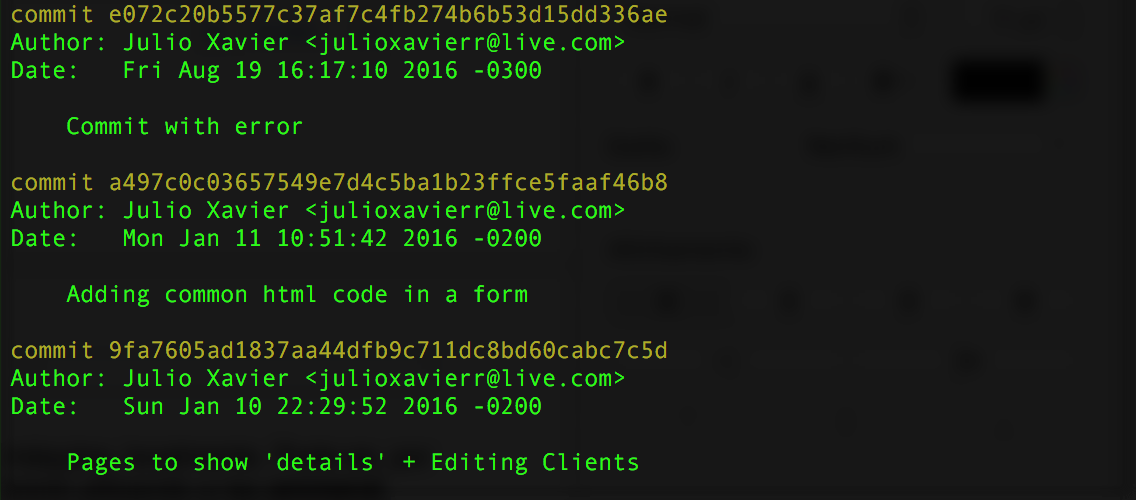
\includegraphics[width=6.25in,height=\textheight]{unidades/unidad1/../../images/git_terminal.png}

}

\caption{Git en Terminal}

\end{figure}%

Se utiliza mediante la \textbf{línea de comandos} o a través de
\textbf{interfaces gráficas} de usuario. Proporciona comandos para
realizar operaciones como:

\begin{enumerate}
\def\labelenumi{\arabic{enumi}.}
\tightlist
\item
  Inicializar un repositorio,
\item
  Realizar cambios,
\item
  Revisar historial,
\item
  Fusionar ramas,
\item
  Entre otros.
\end{enumerate}

\section{¿Para qué sirve Git? 📝}\label{para-quuxe9-sirve-git}

\begin{figure}[H]

{\centering 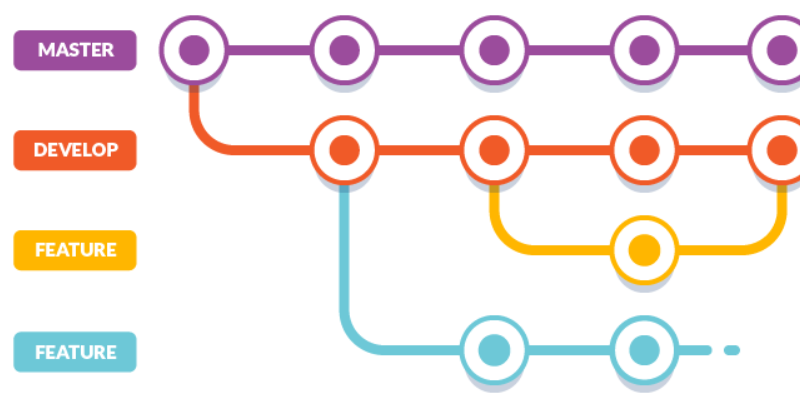
\includegraphics[width=6.25in,height=\textheight]{unidades/unidad1/../../images/seguimiento_cambios_git.png}

}

\caption{Seguimiento de Cambios con Git}

\end{figure}%

Sirve para realizar un seguimiento de los cambios en el código fuente,
coordinar el trabajo entre varios desarrolladores, revertir cambios no
deseados y mantener un historial completo de todas las modificaciones
realizadas en un proyecto.

\section{¿Por qué utilizar Git? 🤔}\label{por-quuxe9-utilizar-git}

\begin{figure}[H]

{\centering 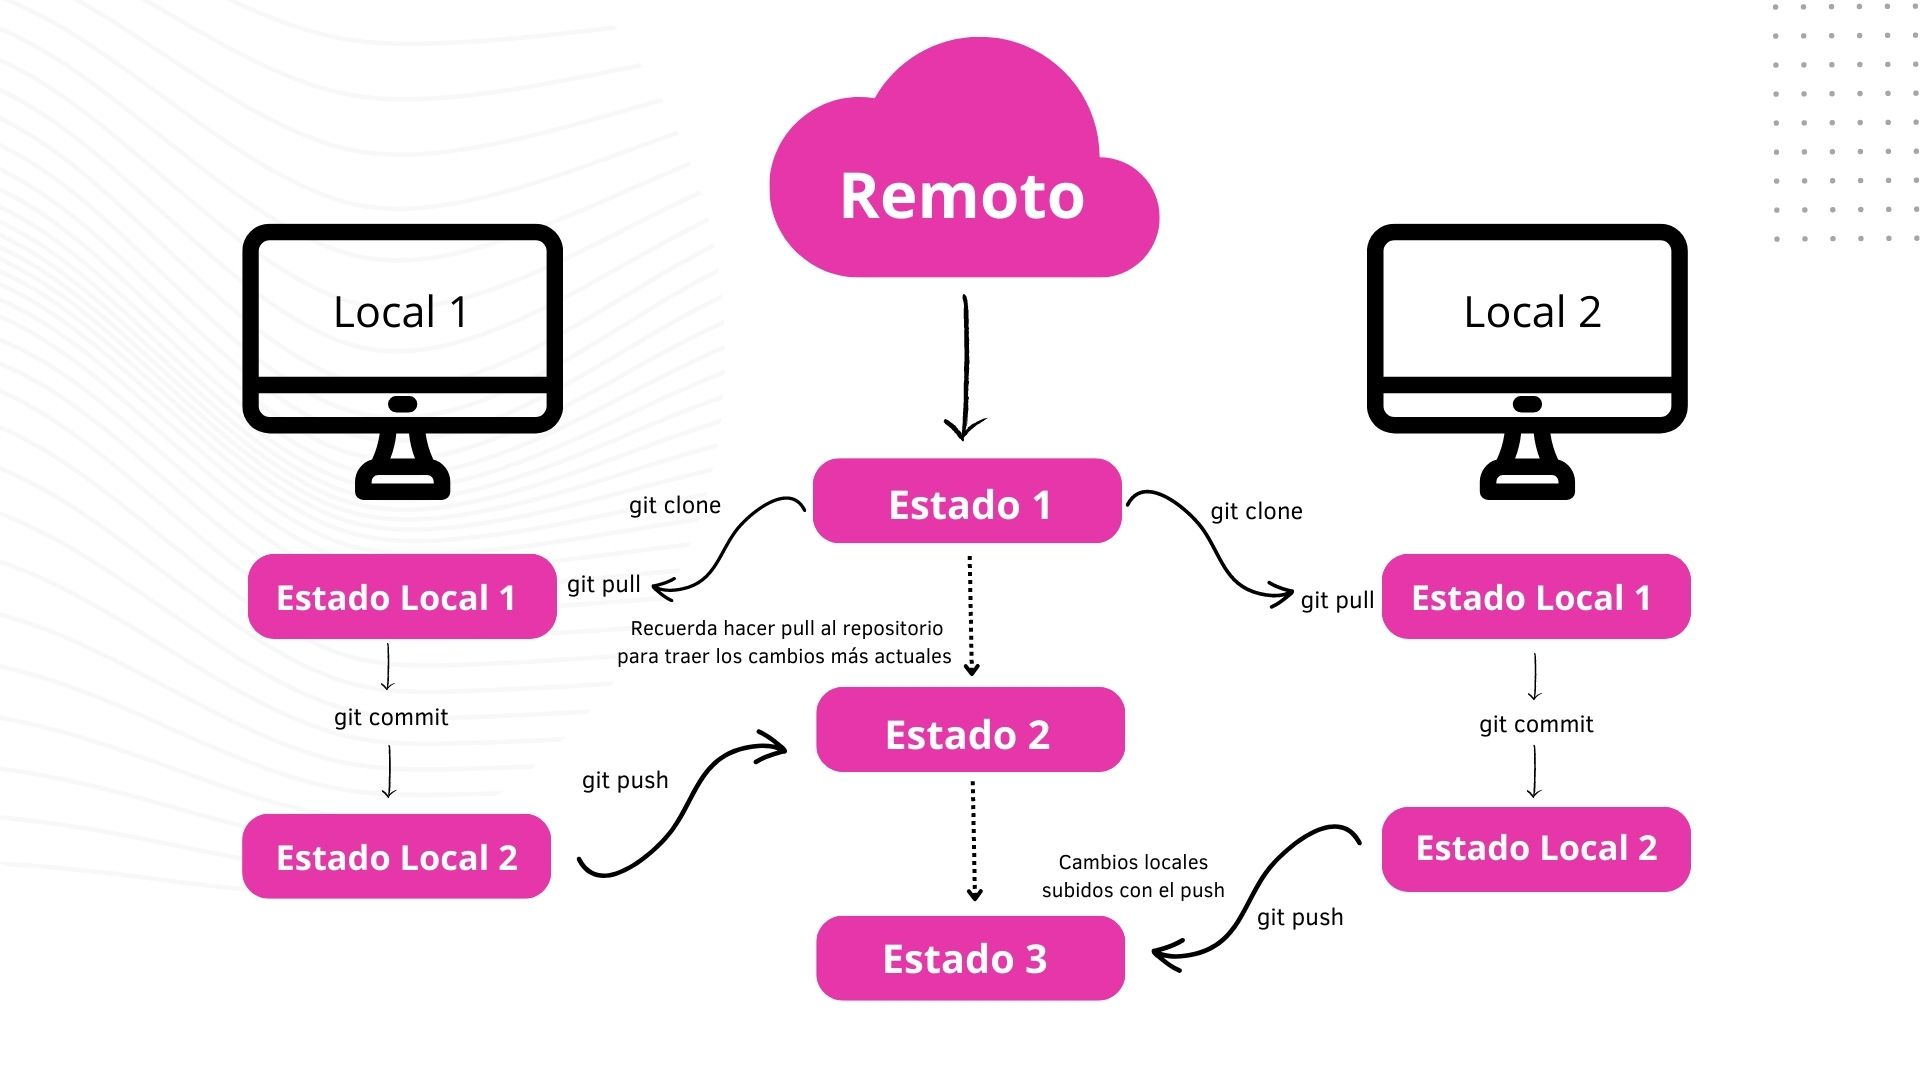
\includegraphics[width=6.25in,height=\textheight]{unidades/unidad1/../../images/ventajas_git.jpg}

}

\caption{Ventajas de Git}

\end{figure}%

Ofrece varias ventajas, como:

\begin{itemize}
\tightlist
\item
  La capacidad de trabajar de forma distribuida
\item
  La gestión eficiente de ramas para desarrollar nuevas funcionalidades
\item
  Corregir errores sin afectar la rama principal
\item
  La posibilidad de colaborar de forma efectiva con otros
  desarrolladores.
\end{itemize}

\section{¿Dónde puedo utilizar Git?
🌐}\label{duxf3nde-puedo-utilizar-git}

\begin{figure}[H]

{\centering 
\includegraphics[width=6.25in,height=\textheight]{unidades/unidad1/../../images/sistemas_operativos_git.png}

}

\caption{Git en Diferentes Sistemas Operativos}

\end{figure}%

Puede ser utilizado en cualquier sistema operativo, incluyendo Windows,
macOS y Linux. Además, es compatible con una amplia variedad de
plataformas de alojamiento de repositorios, siendo GitHub una de las más
populares.

\section{Pasos Básicos 📝}\label{pasos-buxe1sicos}

\begin{tcolorbox}[enhanced jigsaw, bottomrule=.15mm, title=\textcolor{quarto-callout-tip-color}{\faLightbulb}\hspace{0.5em}{Tip}, coltitle=black, leftrule=.75mm, left=2mm, colbacktitle=quarto-callout-tip-color!10!white, breakable, colframe=quarto-callout-tip-color-frame, colback=white, opacitybacktitle=0.6, opacityback=0, bottomtitle=1mm, toptitle=1mm, toprule=.15mm, arc=.35mm, titlerule=0mm, rightrule=.15mm]

Es recomendable tomar en cuenta una herramienta para la edición de
código, como Visual Studio Code, Sublime Text o Atom, para trabajar con
Git y GitHub de manera eficiente.

\end{tcolorbox}

\section{Instalación de Visual Studio Code
📥}\label{instalaciuxf3n-de-visual-studio-code}

\begin{figure}[H]

{\centering 
\includegraphics[width=6.25in,height=\textheight]{unidades/unidad1/../../images/vscode.png}

}

\caption{Visual Studio Code}

\end{figure}%

Si aún no tienes Visual Studio Code instalado, puedes descargarlo desde
\url{https://code.visualstudio.com/download}. Es una herramienta
gratuita y de código abierto que proporciona una interfaz amigable para
trabajar con Git y GitHub.

A continuación se presentan los pasos básicos para utilizar Git y GitHub
en un proyecto de software.

\subsection{Descarga e Instalación de Git
📥}\label{descarga-e-instalaciuxf3n-de-git}

\begin{figure}[H]

{\centering 
\includegraphics[width=6.25in,height=\textheight]{unidades/unidad1/../../images/website-git.png}

}

\caption{Git}

\end{figure}%

\begin{enumerate}
\def\labelenumi{\arabic{enumi}.}
\tightlist
\item
  Visita el sitio web oficial de Git en
  \url{https://git-scm.com/downloads}.
\item
  Descarga el instalador adecuado para tu sistema operativo y sigue las
  instrucciones de instalación.
\end{enumerate}

\subsection{Configuración 🛠️}\label{configuraciuxf3n}

\begin{figure}[H]

{\centering 
\includegraphics[width=6.25in,height=\textheight]{unidades/unidad1/../../images/git_config.png}

}

\caption{Configuración de Git}

\end{figure}%

Una vez instalado Git, es necesario configurar tu nombre de usuario y
dirección de correo electrónico. Esto se puede hacer mediante los
siguientes comandos:

\begin{Shaded}
\begin{Highlighting}[]
\FunctionTok{git}\NormalTok{ config }\AttributeTok{{-}{-}global}\NormalTok{ user.name }\StringTok{"Tu Nombre"}
\FunctionTok{git}\NormalTok{ config }\AttributeTok{{-}{-}global}\NormalTok{ user.email }\StringTok{"tu@email.com"}
\end{Highlighting}
\end{Shaded}

\subsection{Creación de un Repositorio ``helloWorld'' en Python
🐍}\label{creaciuxf3n-de-un-repositorio-helloworld-en-python}

\begin{itemize}
\tightlist
\item
  Crea una nueva carpeta para tu proyecto y ábrela en Visual Studio
  Code.
\item
  Crea un archivo Python llamado \textbf{hello\_world.py} y escribe el
  siguiente código:
\end{itemize}

\begin{Shaded}
\begin{Highlighting}[]
\KeywordTok{def}\NormalTok{ welcome\_message():}
\NormalTok{    name }\OperatorTok{=} \BuiltInTok{input}\NormalTok{(}\StringTok{"Ingrese su nombre: "}\NormalTok{)}
    \BuiltInTok{print}\NormalTok{(}\StringTok{"Bienvenio,"}\NormalTok{, name, }\StringTok{"al curso de Django y React!"}\NormalTok{)}

\ControlFlowTok{if} \VariableTok{\_\_name\_\_} \OperatorTok{==} \StringTok{"\_\_main\_\_"}\NormalTok{:}
\NormalTok{    welcome\_message()}
\end{Highlighting}
\end{Shaded}

\begin{itemize}
\tightlist
\item
  Guarda el archivo y abre una terminal en Visual Studio Code.
\item
  Inicializa un repositorio Git en la carpeta de tu proyecto con el
  siguiente comando:
\end{itemize}

\begin{Shaded}
\begin{Highlighting}[]
\FunctionTok{git}\NormalTok{ init}
\end{Highlighting}
\end{Shaded}

\begin{itemize}
\tightlist
\item
  Añade el archivo al área de preparación con:
\end{itemize}

\begin{Shaded}
\begin{Highlighting}[]
\FunctionTok{git}\NormalTok{ add hello\_world.py}
\end{Highlighting}
\end{Shaded}

\begin{itemize}
\tightlist
\item
  Realiza un commit de los cambios con un mensaje descriptivo:
\end{itemize}

\begin{Shaded}
\begin{Highlighting}[]
\FunctionTok{git}\NormalTok{ commit }\AttributeTok{{-}m} \StringTok{"Añadir archivo hello\_world.py"}
\end{Highlighting}
\end{Shaded}

\subsection{Comandos Básicos de Git
📝}\label{comandos-buxe1sicos-de-git}

\begin{itemize}
\tightlist
\item
  \textbf{git init:} Inicializa un nuevo repositorio Git.
\item
  \textbf{git add :} Añade un archivo al área de preparación.
\item
  \textbf{git commit -m ``''}: Realiza un commit de los cambios con un
  mensaje descriptivo.
\item
  \textbf{git push:} Sube los cambios al repositorio remoto.
\item
  \textbf{git pull:} Descarga cambios del repositorio remoto.
\item
  \textbf{git branch:} Lista las ramas disponibles.
\item
  \textbf{git checkout :} Cambia a una rama específica.
\item
  \textbf{git merge :} Fusiona una rama con la rama actual.
\item
  \textbf{git reset :} Descarta los cambios en un archivo.
\item
  \textbf{git diff:} Muestra las diferencias entre versiones.
\end{itemize}

\subsection{Estados en Git 📊}\label{estados-en-git}

\begin{itemize}
\tightlist
\item
  \textbf{Local:} Representa los cambios que realizas en tu repositorio
  local antes de hacer un commit. Estos cambios están únicamente en tu
  máquina.
\item
  \textbf{Staging:} Indica los cambios que has añadido al área de
  preparación con el comando \texttt{git\ add}. Estos cambios están
  listos para ser confirmados en el próximo commit.
\item
  \textbf{Commit:} Son los cambios que has confirmado en tu repositorio
  local con el comando \texttt{git\ commit}. Estos cambios se han
  guardado de manera permanente en tu repositorio local.
\item
  \textbf{Server:} Son los cambios que has subido al repositorio remoto
  con el comando \texttt{git\ push}. Estos cambios están disponibles
  para otros colaboradores del proyecto.
\end{itemize}

\begin{center}\rule{0.5\linewidth}{0.5pt}\end{center}

\chapter{Tutorial: Moviendo Cambios entre Estados en Git
📝}\label{tutorial-moviendo-cambios-entre-estados-en-git}

\section{Introducción}\label{introducciuxf3n}

En este tutorial, aprenderemos a utilizar Git para gestionar cambios en
nuestro proyecto y moverlos entre diferentes estados. Utilizaremos un
ejemplo práctico para comprender mejor estos conceptos.

\begin{Shaded}
\begin{Highlighting}[]
\KeywordTok{def}\NormalTok{ welcome\_message():}
\NormalTok{    name }\OperatorTok{=} \BuiltInTok{input}\NormalTok{(}\StringTok{"Ingrese su nombre: "}\NormalTok{)}
    \BuiltInTok{print}\NormalTok{(}\StringTok{"Bienvenio,"}\NormalTok{, name, }\StringTok{"al curso de Django y React!"}\NormalTok{)}

\ControlFlowTok{if} \VariableTok{\_\_name\_\_} \OperatorTok{==} \StringTok{"\_\_main\_\_"}\NormalTok{:}
\NormalTok{    welcome\_message()}
\end{Highlighting}
\end{Shaded}

\section{Sección 1: Modificar Archivos en el
Repositorio}\label{secciuxf3n-1-modificar-archivos-en-el-repositorio}

En esta sección, aprenderemos cómo realizar cambios en nuestros archivos
y reflejarlos en Git.

\section{Mover Cambios de Local a
Staging:}\label{mover-cambios-de-local-a-staging}

\begin{enumerate}
\def\labelenumi{\arabic{enumi}.}
\tightlist
\item
  Abre el archivo \textbf{hello\_world.py} en Visual Studio Code.
\item
  Modifica el mensaje de bienvenida a ``Bienvenido'' en lugar de
  ``Bienvenio''.
\item
  Guarda los cambios y abre una terminal en Visual Studio Code.
\end{enumerate}

Hemos corregido un error en nuestro archivo y queremos reflejarlo en
Git.

\begin{Shaded}
\begin{Highlighting}[]
\ExtensionTok{def}\NormalTok{ welcome\_message}\ErrorTok{(}\KeywordTok{)}\BuiltInTok{:}
    \ExtensionTok{name}\NormalTok{ = input}\ErrorTok{(}\StringTok{"Ingrese su nombre: "}\KeywordTok{)}
    \ExtensionTok{print}\ErrorTok{(}\StringTok{"Bienvenido,"}\ExtensionTok{,}\NormalTok{ name, }\StringTok{"al curso de Django y React!"}\KeywordTok{)}

\ControlFlowTok{if} \ExtensionTok{\_\_name\_\_}\NormalTok{ == }\StringTok{"\_\_main\_\_"}\NormalTok{:}
    \FunctionTok{welcome\_message()}
\end{Highlighting}
\end{Shaded}

\section{Agregar Cambios de Local a
Staging:}\label{agregar-cambios-de-local-a-staging}

\begin{Shaded}
\begin{Highlighting}[]
\FunctionTok{git}\NormalTok{ add hello\_world.py}
\end{Highlighting}
\end{Shaded}

Hemos añadido los cambios al área de preparación y están listos para ser
confirmados en el próximo commit.

\section{Sección 2: Confirmar Cambios en un
Commit}\label{secciuxf3n-2-confirmar-cambios-en-un-commit}

En esta sección, aprenderemos cómo confirmar los cambios en un commit y
guardarlos de manera permanente en nuestro repositorio.

\section{Mover Cambios de Staging a
Commit:}\label{mover-cambios-de-staging-a-commit}

\begin{Shaded}
\begin{Highlighting}[]
\FunctionTok{git}\NormalTok{ commit }\AttributeTok{{-}m} \StringTok{"Corregir mensaje de bienvenida"}
\end{Highlighting}
\end{Shaded}

Hemos confirmado los cambios en un commit con un mensaje descriptivo.

\section{Sección 3: Creación y Fusión de
Ramas}\label{secciuxf3n-3-creaciuxf3n-y-fusiuxf3n-de-ramas}

En esta sección, aprenderemos cómo crear y fusionar ramas en Git para
desarrollar nuevas funcionalidades de forma aislada.

\section{Crear una Nueva Rama:}\label{crear-una-nueva-rama}

\begin{Shaded}
\begin{Highlighting}[]
\FunctionTok{git}\NormalTok{ branch feature}
\end{Highlighting}
\end{Shaded}

Hemos creado una nueva rama llamada ``feature'' para desarrollar una
nueva funcionalidad.

\section{Implementar Funcionalidades en la
Rama:}\label{implementar-funcionalidades-en-la-rama}

\begin{enumerate}
\def\labelenumi{\arabic{enumi}.}
\tightlist
\item
  Abre el archivo \textbf{hello\_world.py} en Visual Studio Code.
\item
  Añade una nueva función para mostrar un mensaje de despedida.
\item
  Guarda los cambios y abre una terminal en Visual Studio Code.
\item
  Añade los cambios al área de preparación y confírmalos en un commit.
\item
  Cambia a la rama principal con \texttt{git\ checkout\ main}.
\end{enumerate}

\section{Fusionar Ramas con la Rama
Principal:}\label{fusionar-ramas-con-la-rama-principal}

\begin{Shaded}
\begin{Highlighting}[]
\FunctionTok{git}\NormalTok{ merge feature}
\end{Highlighting}
\end{Shaded}

Hemos fusionado la rama ``feature'' con la rama principal y añadido la
nueva funcionalidad al proyecto.

\section{Sección 4: Revertir Cambios en un
Archivo}\label{secciuxf3n-4-revertir-cambios-en-un-archivo}

En esta sección, aprenderemos cómo revertir cambios en un archivo y
deshacerlos en Git.

\section{Revertir Cambios en un
Archivo:}\label{revertir-cambios-en-un-archivo}

\begin{Shaded}
\begin{Highlighting}[]
\FunctionTok{git}\NormalTok{ reset hello\_world.py}
\end{Highlighting}
\end{Shaded}

Hemos revertido los cambios en el archivo \textbf{hello\_world.py} y
deshecho las modificaciones realizadas.

\section{Conclusión}\label{conclusiuxf3n}

En este tutorial, hemos aprendido a gestionar cambios en nuestro
proyecto y moverlos entre diferentes estados en Git. Estos conceptos son
fundamentales para trabajar de forma eficiente en proyectos de software
y colaborar con otros desarrolladores.

\chapter{Asignación}\label{asignaciuxf3n}

\href{https://classroom.github.com/a/o-qydr2W}{Hello World!}

Este proyecto de ejemplo está escrito en Python y se prueba con pytest.

\textbf{La Asignación}

Las pruebas están fallando en este momento porque el método no está
devolviendo la cadena correcta. Corrige el código del archivo
\textbf{hello.py} para que las pruebas sean exitosas, debe devolver la
cadena correcta \textbf{``Hello World!''}x

El comando de ejecución del test es:

\begin{Shaded}
\begin{Highlighting}[]
\ExtensionTok{pytest}\NormalTok{ test\_hello.py}
\end{Highlighting}
\end{Shaded}

¡Mucha suerte!

\chapter{GitHub Classroom 📒}\label{github-classroom}

\begin{figure}[H]

{\centering 
\includegraphics[width=1.04167in,height=\textheight]{unidades/unidad1/../../images/github classroom.png}

}

\caption{Github Classroom}

\end{figure}%

GitHub Classroom es una herramienta poderosa que facilita la gestión de
tareas y asignaciones en GitHub, especialmente diseñada para entornos
educativos.

\section{¿Qué es GitHub Classroom? 🤔}\label{quuxe9-es-github-classroom}

\begin{figure}[H]

{\centering 
\includegraphics[width=4.16667in,height=\textheight]{unidades/unidad1/../../images/github-classroom-ventana.jpg}

}

\caption{Github Classroom Windows}

\end{figure}%

GitHub Classroom es una extensión de GitHub que permite a los profesores
crear y gestionar asignaciones utilizando repositorios de GitHub.
Proporciona una forma organizada y eficiente de distribuir tareas a los
estudiantes, recopilar y revisar su trabajo, y proporcionar
retroalimentación.

\subsection{Funcionalidades Principales
⚙️}\label{funcionalidades-principales}

\textbf{Creación de Asignaciones:} Los profesores pueden crear tareas y
asignaciones directamente desde GitHub Classroom, proporcionando
instrucciones detalladas y estableciendo criterios de evaluación.

\textbf{Distribución Automatizada:} Una vez que se crea una asignación,
GitHub Classroom genera automáticamente repositorios privados para cada
estudiante o equipo, basándose en una plantilla predefinida.

\textbf{Seguimiento de Progreso:} Los profesores pueden realizar un
seguimiento del progreso de los estudiantes y revisar sus contribuciones
a través de solicitudes de extracción (pull requests) y comentarios en
el código.

\textbf{Revisión y Retroalimentación:} Los estudiantes envían sus
trabajos a través de solicitudes de extracción, lo que permite a los
profesores revisar y proporcionar retroalimentación específica sobre su
código.

\section{Ejemplo Práctico}\label{ejemplo-pruxe1ctico}

\subsection{Creación de una Asignación en GitHub Classroom
📒}\label{creaciuxf3n-de-una-asignaciuxf3n-en-github-classroom}

\textbf{Iniciar Sesión:} Ingresa a GitHub Classroom con tu cuenta de
GitHub y selecciona la opción para crear una nueva asignación.

\begin{center}
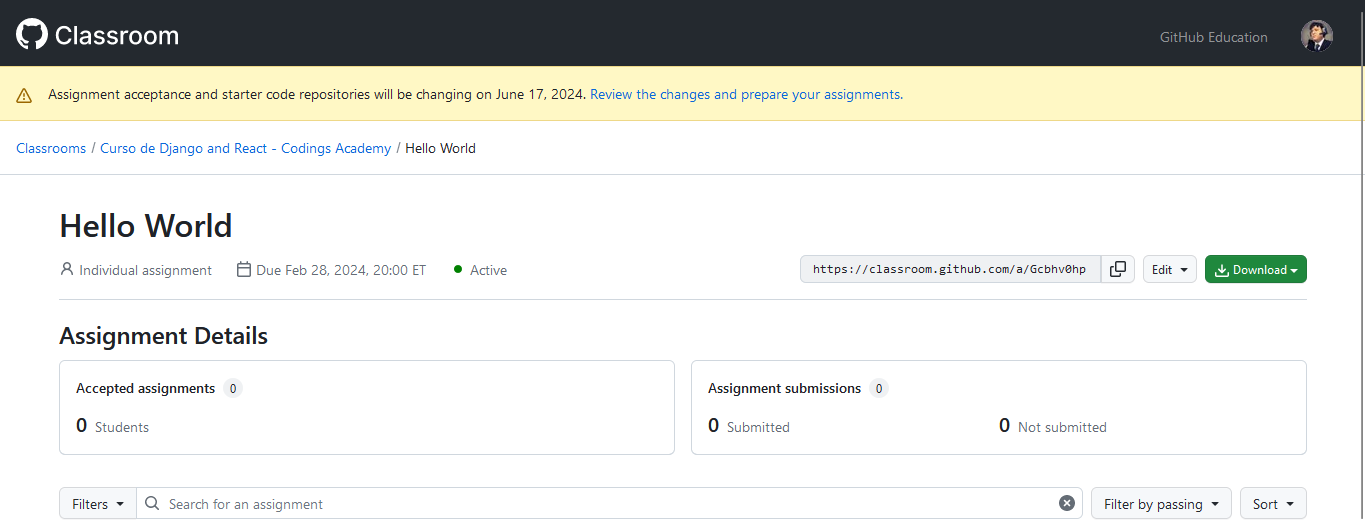
\includegraphics{unidades/unidad1/images/paste-2.png}
\end{center}

\textbf{Definir la Tarea:} Proporciona instrucciones claras y detalladas
sobre la tarea, incluyendo cualquier código base o recursos necesarios.
Establece los criterios de evaluación para guiar a los estudiantes.

\begin{center}
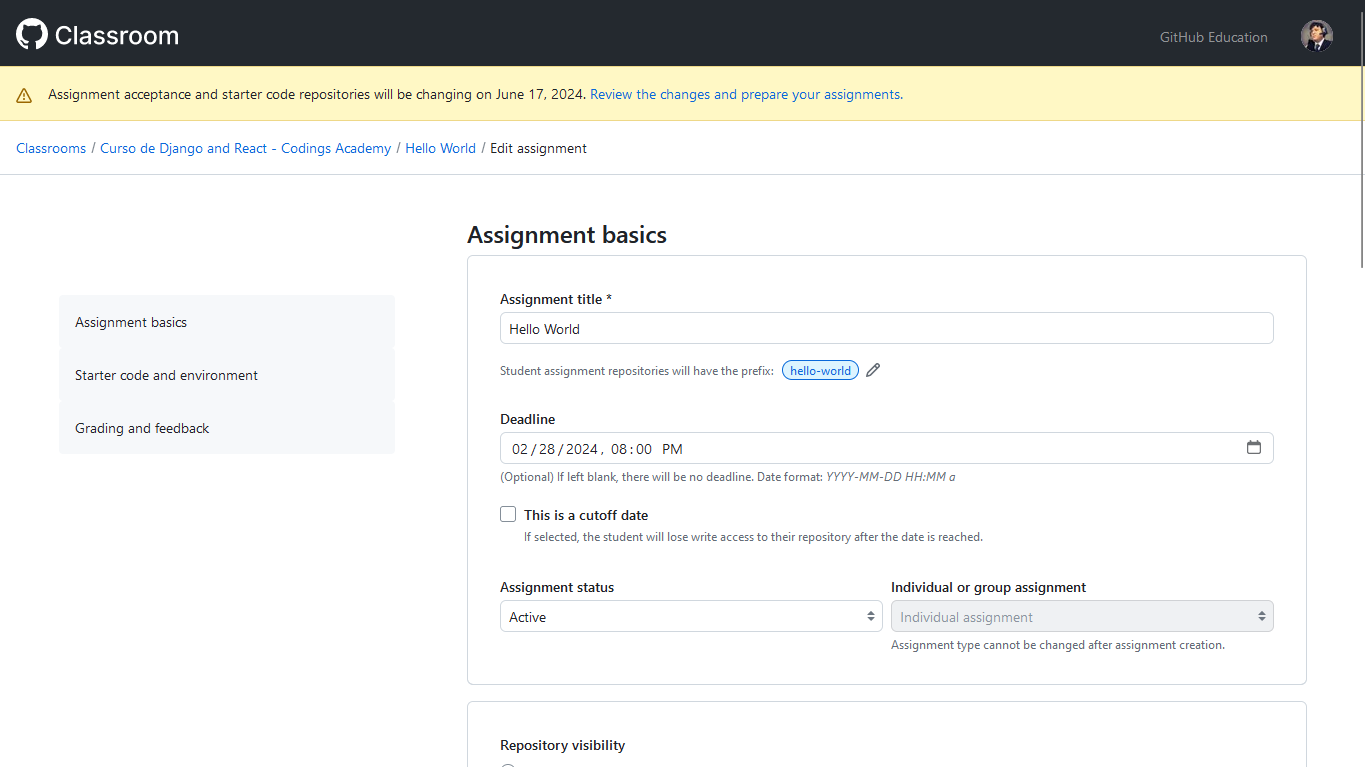
\includegraphics{unidades/unidad1/images/paste-1.png}
\end{center}

\textbf{Configurar la Plantilla:} Selecciona una plantilla de
repositorio existente o crea una nueva plantilla que servirá como base
para los repositorios de los estudiantes.

\begin{center}
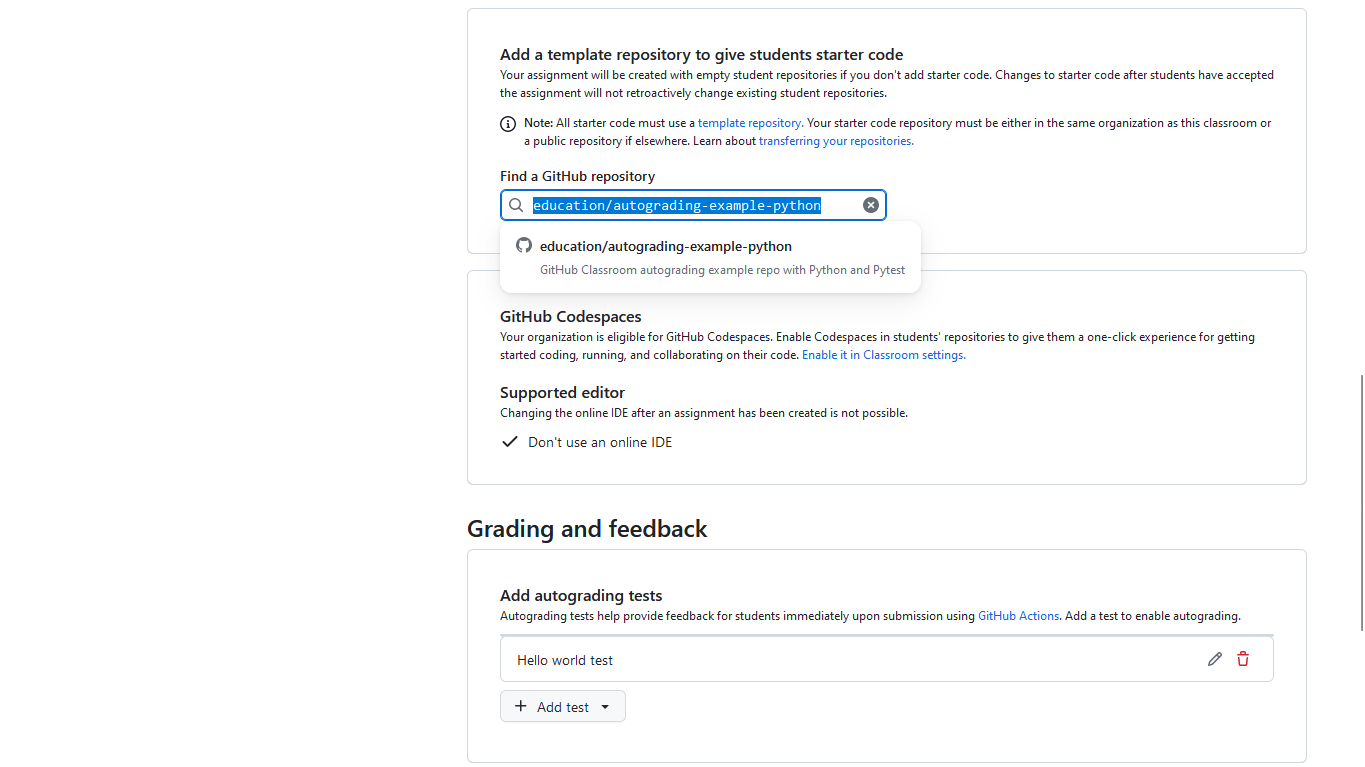
\includegraphics{unidades/unidad1/images/paste-3.png}
\end{center}

\textbf{Distribuir la Asignación:} Una vez configurada la asignación,
comparte el enlace generado con tus estudiantes para que puedan acceder
a sus repositorios privados.

\begin{center}
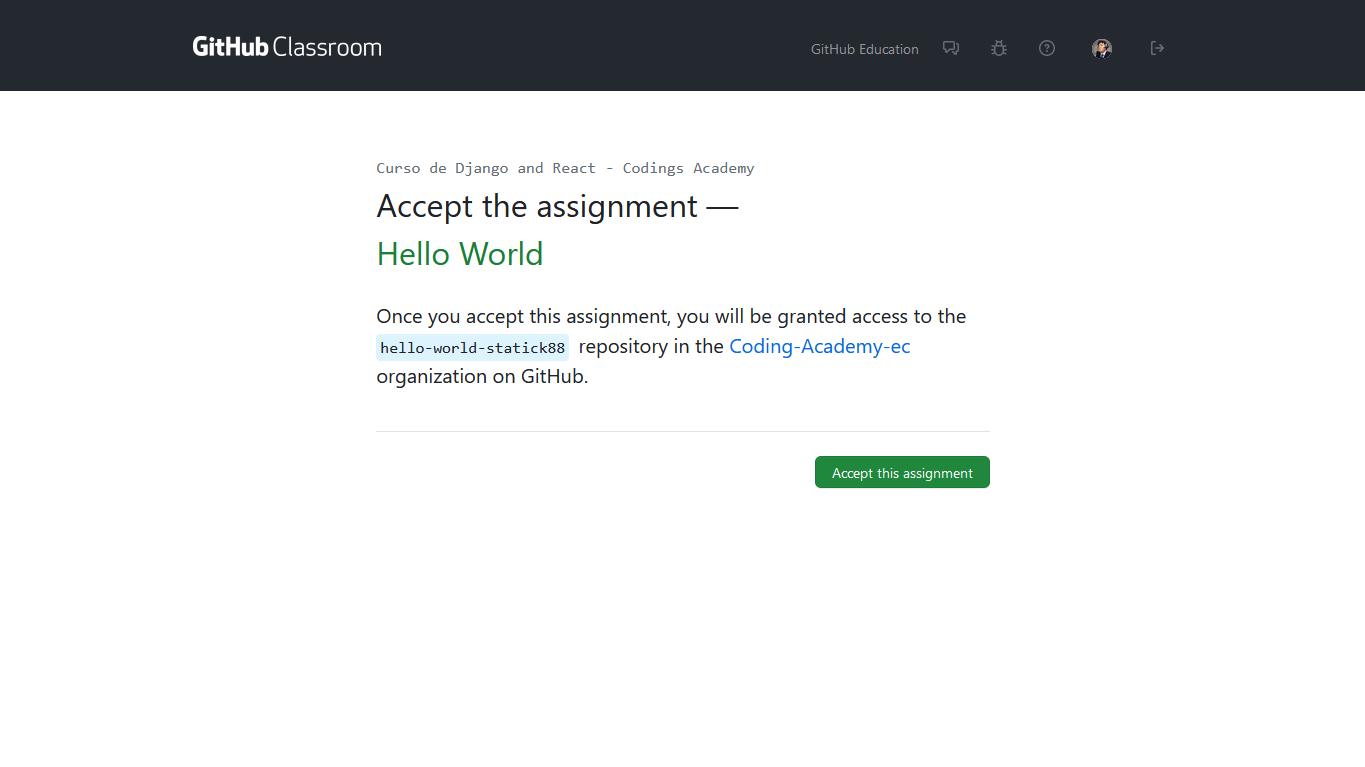
\includegraphics{unidades/unidad1/images/paste-4.png}
\end{center}

\section{Trabajo de los Estudiantes
🧑‍💻}\label{trabajo-de-los-estudiantes}

\textbf{Aceptar la Asignación:} Los estudiantes reciben el enlace de la
asignación y aceptan la tarea, lo que les permite crear un repositorio
privado basado en la plantilla proporcionada.

\begin{center}
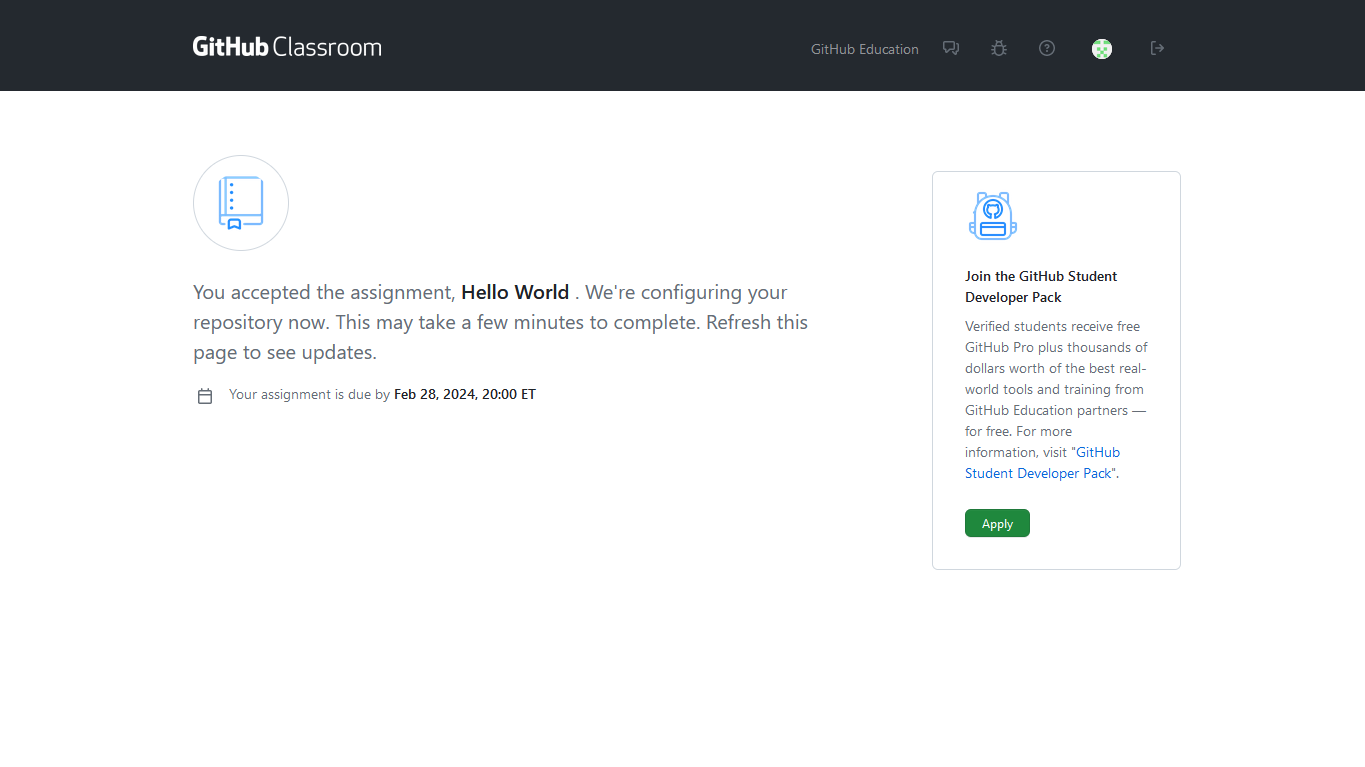
\includegraphics{unidades/unidad1/images/paste-6.png}
\end{center}

\textbf{Actualizar el Navegador:} Los estudiantes actualizan su
navegador para ver el nuevo repositorio creado en su cuenta de GitHub.

\begin{center}
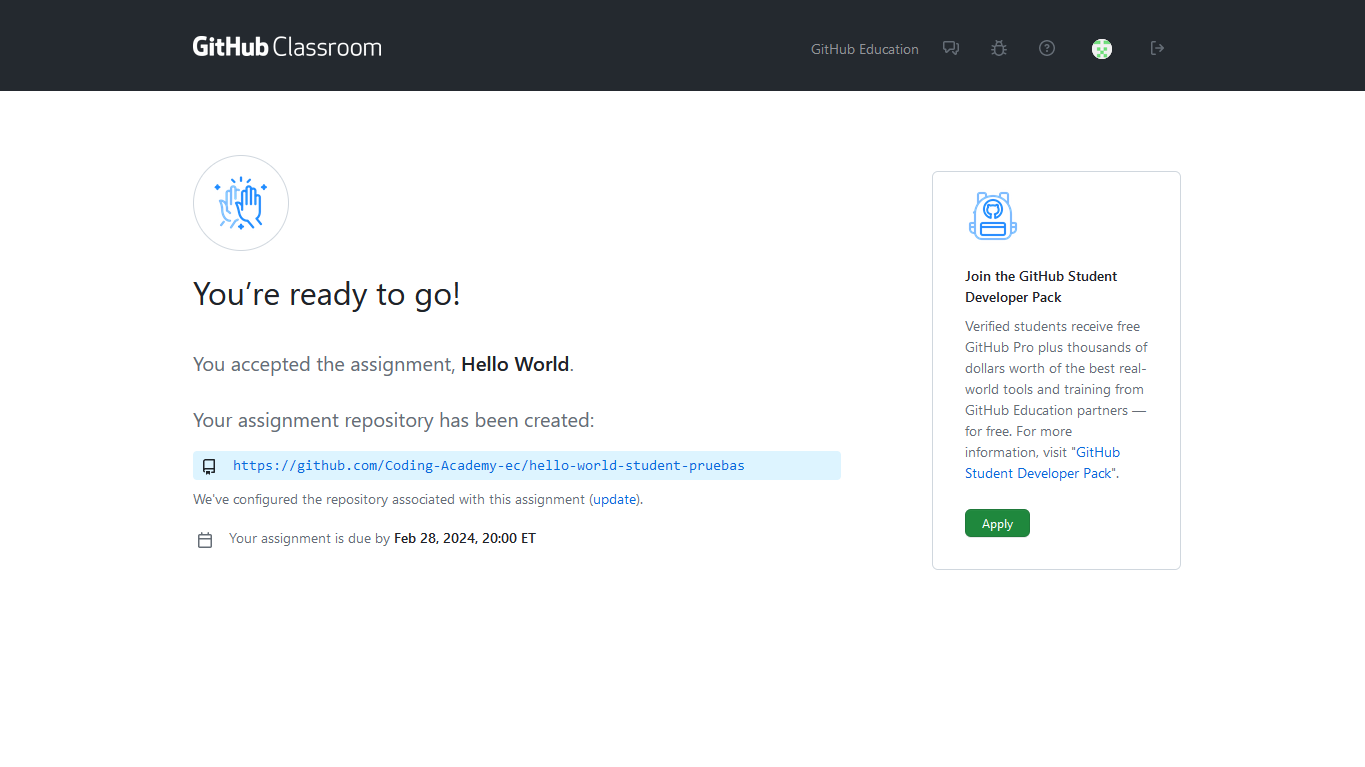
\includegraphics{unidades/unidad1/images/paste-8.png}
\end{center}

\textbf{Clonar el Repositorio:} Los estudiantes clonan el repositorio
asignado en su computadora local utilizando el enlace proporcionado.

\begin{center}
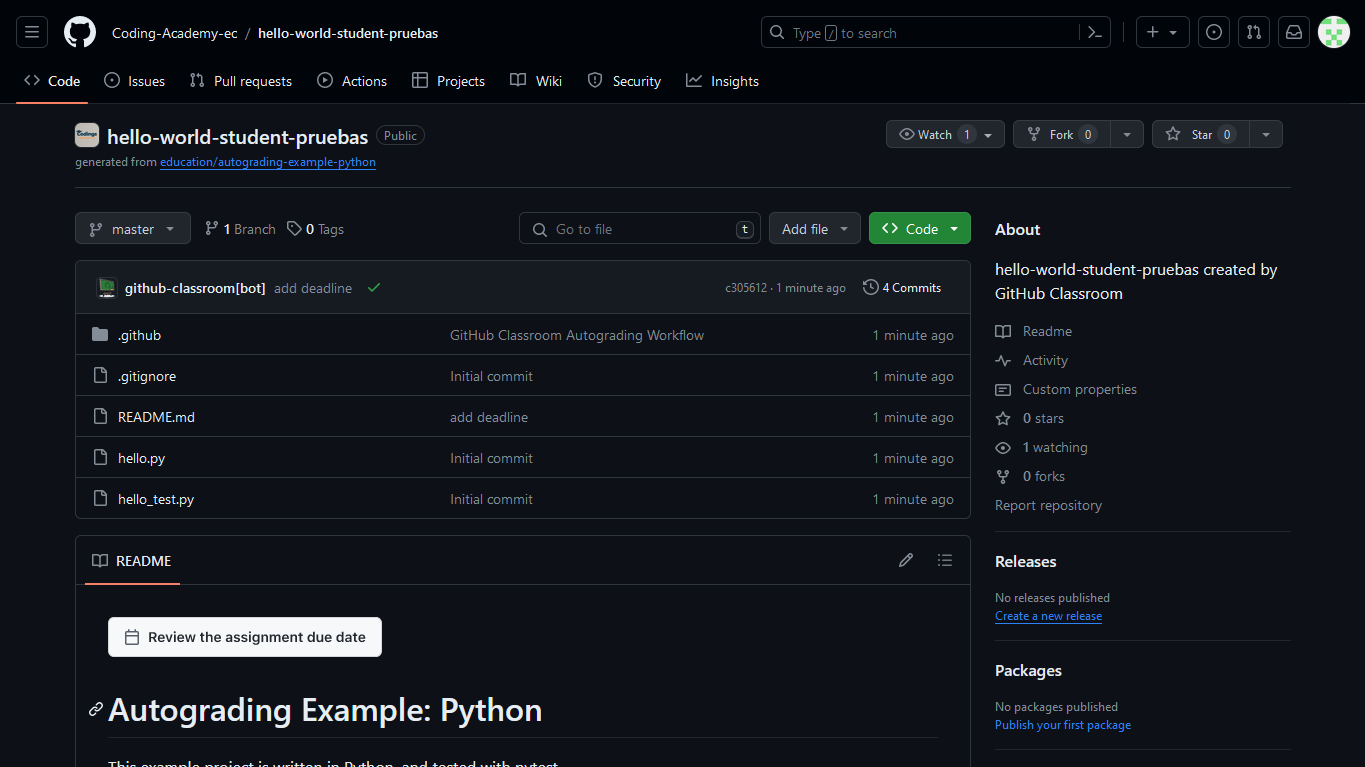
\includegraphics{unidades/unidad1/images/paste-9.png}
\end{center}

Utilizar el comando git clone: Aplique el comando git clone para clonar
el repositorio en su computadora local.

\begin{Shaded}
\begin{Highlighting}[]
\FunctionTok{git}\NormalTok{ clone }\OperatorTok{\textless{}}\NormalTok{enlace{-}del{-}repositorio}\OperatorTok{\textgreater{}}
\end{Highlighting}
\end{Shaded}

\begin{center}
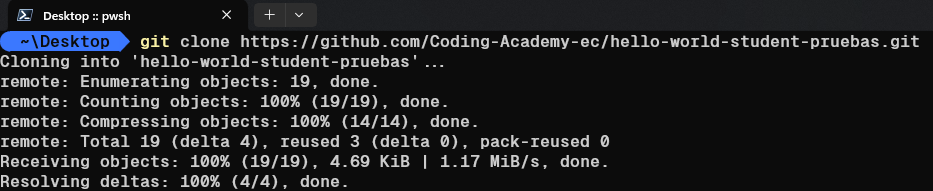
\includegraphics{unidades/unidad1/images/paste-10.png}
\end{center}

\textbf{Desarrollar la Tarea:} Los estudiantes trabajan en la tarea,
realizando los cambios necesarios y realizando commits de manera regular
para mantener un historial de su trabajo.

\begin{tcolorbox}[enhanced jigsaw, bottomrule=.15mm, title=\textcolor{quarto-callout-tip-color}{\faLightbulb}\hspace{0.5em}{Tip}, coltitle=black, leftrule=.75mm, left=2mm, colbacktitle=quarto-callout-tip-color!10!white, breakable, colframe=quarto-callout-tip-color-frame, colback=white, opacitybacktitle=0.6, opacityback=0, bottomtitle=1mm, toptitle=1mm, toprule=.15mm, arc=.35mm, titlerule=0mm, rightrule=.15mm]

Puedes probar el test incorporado con el comando \texttt{pytest} en la
terminal, para verificar que el código cumple con los requerimientos

\end{tcolorbox}

\begin{Shaded}
\begin{Highlighting}[]
\ExtensionTok{pytest}
\end{Highlighting}
\end{Shaded}

Una vez desarrollado el código de acuerdo a la asignación en local
deberían pasar el o los test

\begin{center}
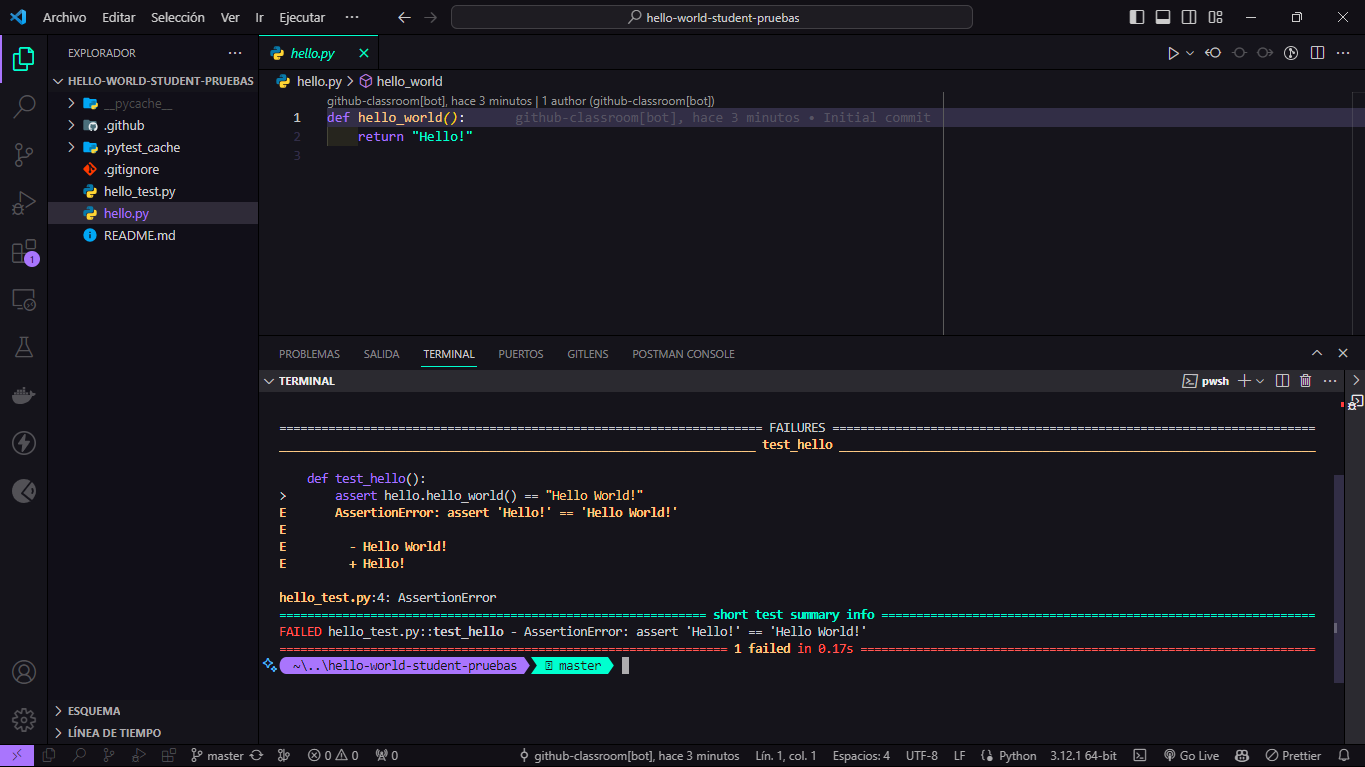
\includegraphics{unidades/unidad1/images/paste-11.png}
\end{center}

\textbf{Enviar la Solicitud de Extracción:} Una vez completada la tarea,
los estudiantes envían una solicitud de extracción desde su rama hacia
la rama principal del repositorio, solicitando la revisión del profesor.

\begin{center}
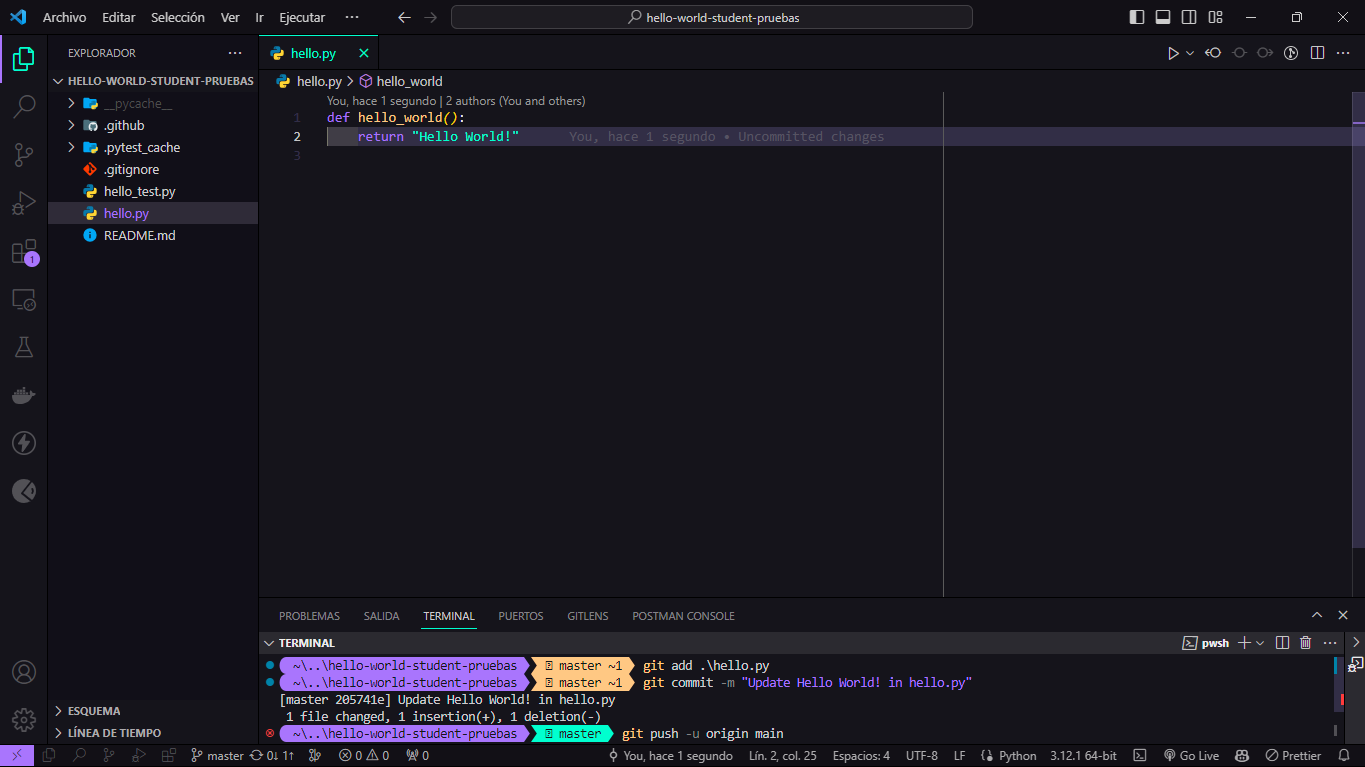
\includegraphics{unidades/unidad1/images/paste-12.png}
\end{center}

Una vez realizado el \texttt{push} se envía al respositorio principal y
se ejecutan los test en Github

\begin{tcolorbox}[enhanced jigsaw, bottomrule=.15mm, title=\textcolor{quarto-callout-tip-color}{\faLightbulb}\hspace{0.5em}{Tip}, coltitle=black, leftrule=.75mm, left=2mm, colbacktitle=quarto-callout-tip-color!10!white, breakable, colframe=quarto-callout-tip-color-frame, colback=white, opacitybacktitle=0.6, opacityback=0, bottomtitle=1mm, toptitle=1mm, toprule=.15mm, arc=.35mm, titlerule=0mm, rightrule=.15mm]

Se recomienda hacer las pruebas en local antes de enviar los cambios al
respositorio en Github

\end{tcolorbox}

\begin{center}
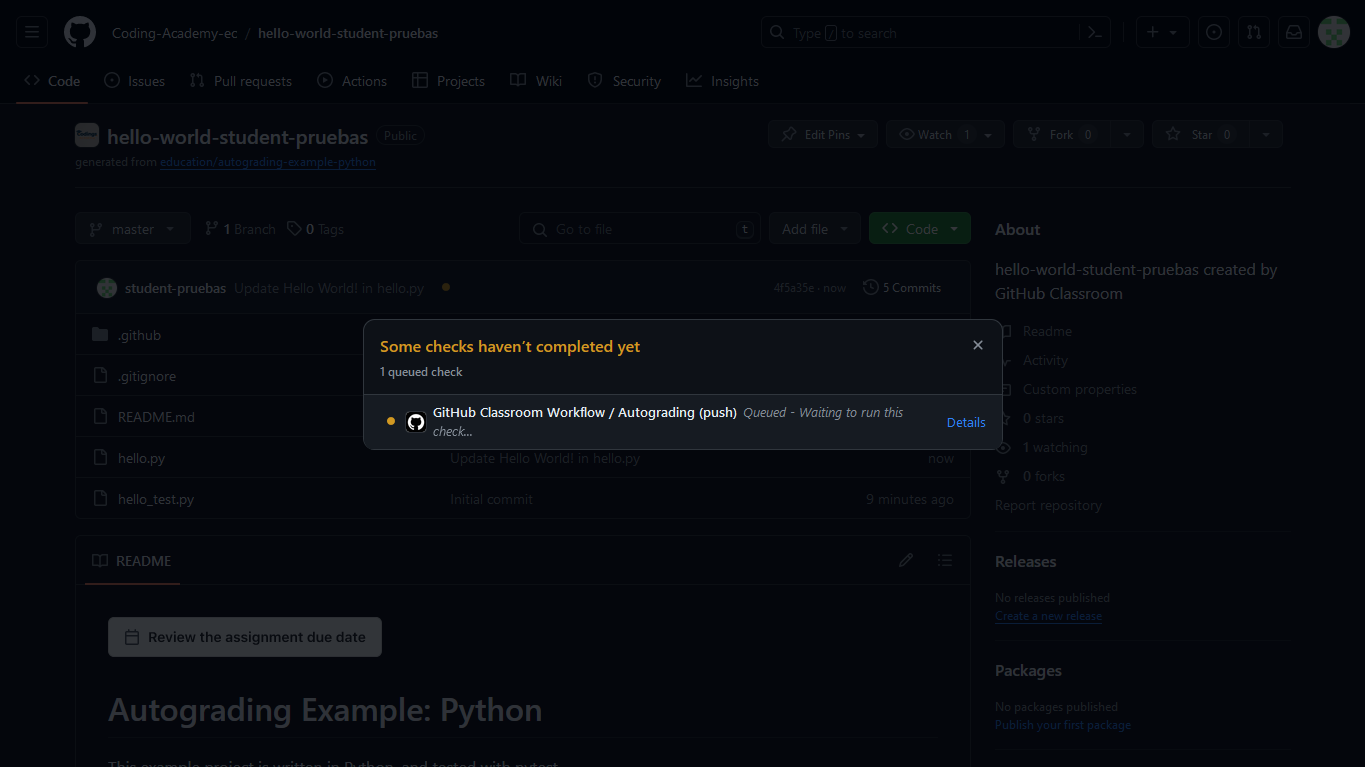
\includegraphics{unidades/unidad1/images/paste-13.png}
\end{center}

Este Action lo que hace es evaluar los cambios realizados

\begin{center}
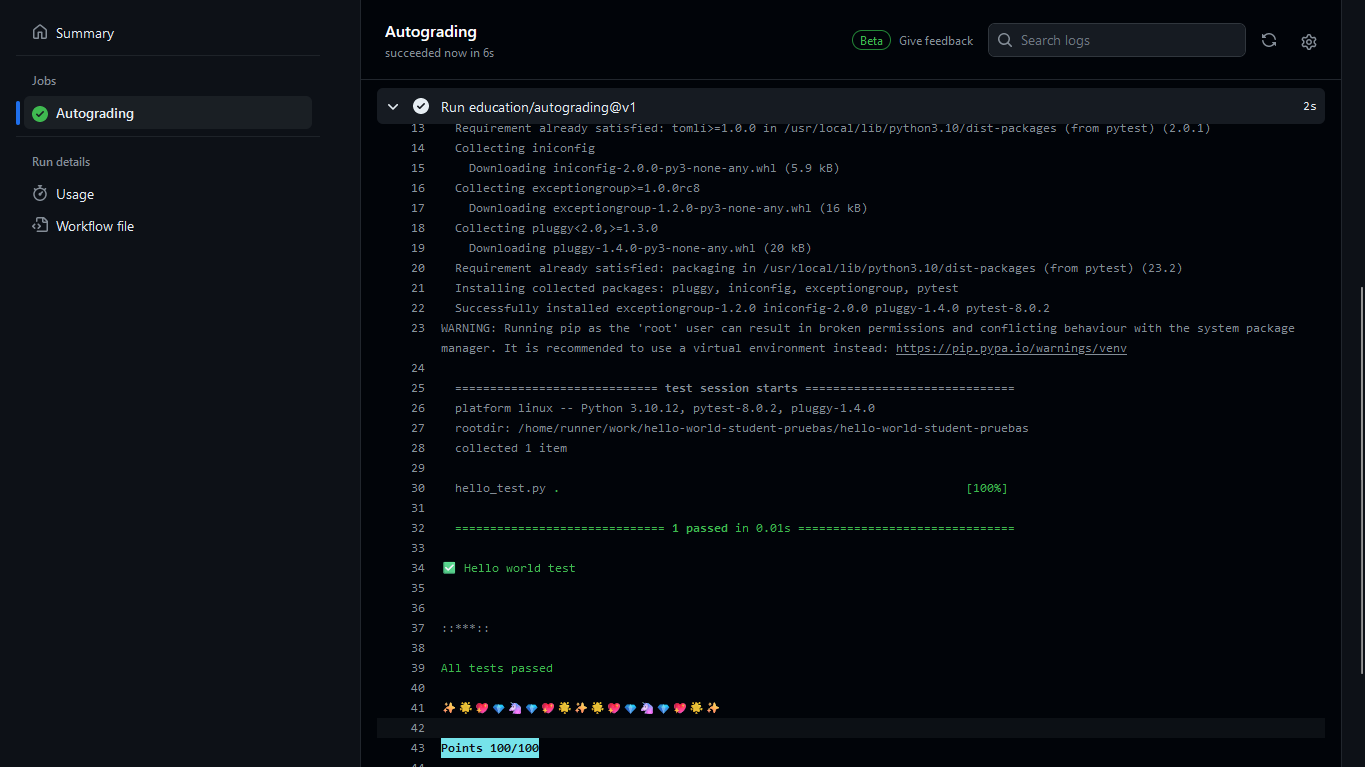
\includegraphics{unidades/unidad1/images/paste-14.png}
\end{center}

\begin{tcolorbox}[enhanced jigsaw, bottomrule=.15mm, title=\textcolor{quarto-callout-tip-color}{\faLightbulb}\hspace{0.5em}{Tip}, coltitle=black, leftrule=.75mm, left=2mm, colbacktitle=quarto-callout-tip-color!10!white, breakable, colframe=quarto-callout-tip-color-frame, colback=white, opacitybacktitle=0.6, opacityback=0, bottomtitle=1mm, toptitle=1mm, toprule=.15mm, arc=.35mm, titlerule=0mm, rightrule=.15mm]

Se recomienda hacer las pruebas en local antes de enviar los cambios al
respositorio en Github

\end{tcolorbox}

\textbf{Revisión y Retroalimentación:} Los profesores revisan las
solicitudes de extracción, proporcionan comentarios sobre el código y
evalúan el trabajo de los estudiantes según los criterios establecidos.

\begin{center}
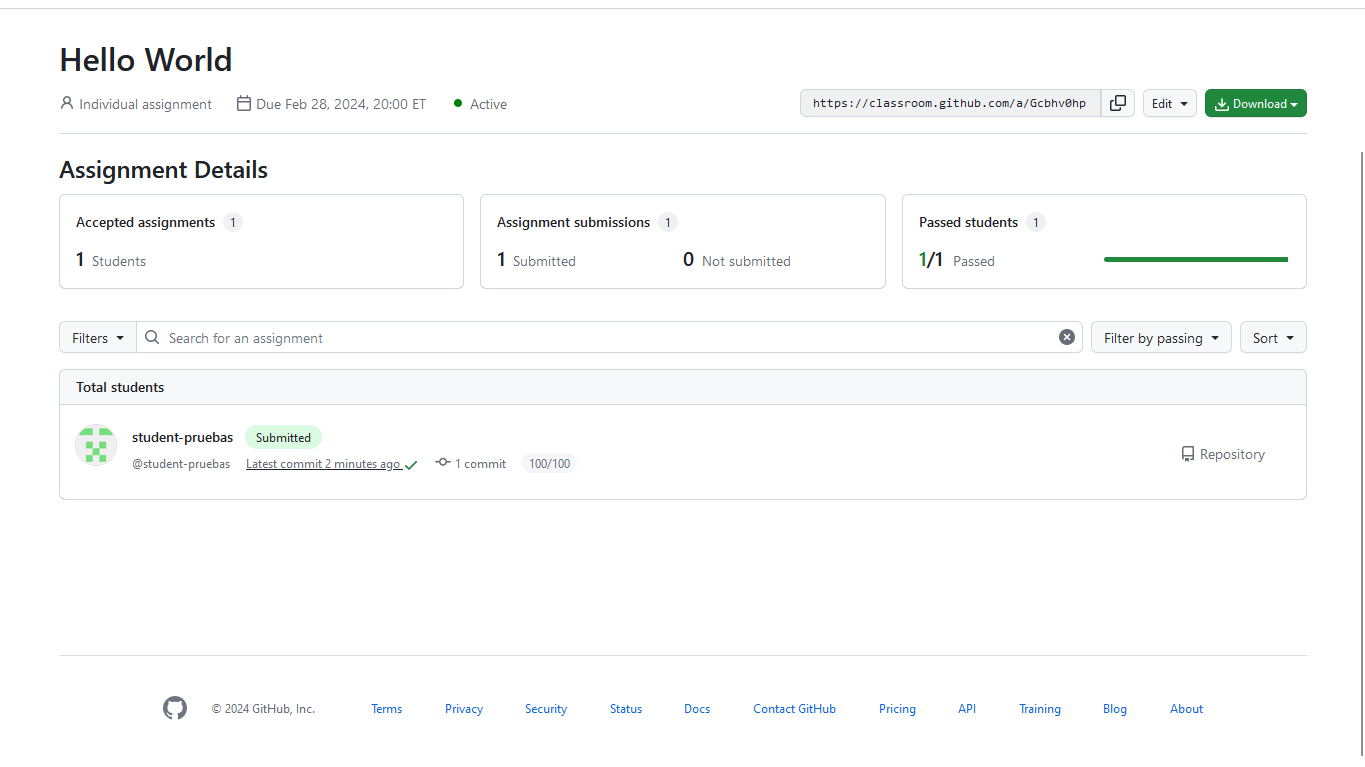
\includegraphics{unidades/unidad1/images/paste-15.png}
\end{center}

\begin{tcolorbox}[enhanced jigsaw, bottomrule=.15mm, title=\textcolor{quarto-callout-tip-color}{\faLightbulb}\hspace{0.5em}{Tip}, coltitle=black, leftrule=.75mm, left=2mm, colbacktitle=quarto-callout-tip-color!10!white, breakable, colframe=quarto-callout-tip-color-frame, colback=white, opacitybacktitle=0.6, opacityback=0, bottomtitle=1mm, toptitle=1mm, toprule=.15mm, arc=.35mm, titlerule=0mm, rightrule=.15mm]

\textbf{GitHub Classroom} ofrece una manera eficiente y organizada de
administrar tareas y asignaciones en entornos educativos, fomentando la
colaboración, el aprendizaje y la retroalimentación efectiva entre
profesores y estudiantes.

\end{tcolorbox}

\chapter{Docker 🐋}\label{docker}

\begin{figure}[H]

{\centering 
\includegraphics[width=1.04167in,height=\textheight]{unidades/unidad1/../../images/docker-logo.png}

}

\caption{Docker}

\end{figure}%

Docker es una plataforma de código abierto que permite a los
desarrolladores empaquetar, distribuir y ejecutar aplicaciones en
contenedores. Los contenedores son entornos ligeros y portátiles que
incluyen todo lo necesario para ejecutar una aplicación de forma
consistente en cualquier entorno.

\chapter{Conceptos Básicos de Docker
📒}\label{conceptos-buxe1sicos-de-docker}

\section{Imagen}\label{imagen}

\begin{Shaded}
\begin{Highlighting}[]
\ExtensionTok{docker}\NormalTok{ pull python:3.9{-}slim}
\end{Highlighting}
\end{Shaded}

Una imagen de Docker es un paquete de software ligero y portátil que
incluye todo lo necesario para ejecutar una aplicación, incluidos el
código, las bibliotecas y las dependencias. Las imágenes se utilizan
como plantillas para crear contenedores.

\section{Contenedor 📦}\label{contenedor}

\begin{Shaded}
\begin{Highlighting}[]
\ExtensionTok{docker}\NormalTok{ run }\AttributeTok{{-}d} \AttributeTok{{-}p}\NormalTok{ 5000:5000 myapp}
\end{Highlighting}
\end{Shaded}

Un contenedor de Docker es una instancia en tiempo de ejecución de una
imagen de Docker. Los contenedores son entornos aislados que ejecutan
aplicaciones de forma independiente y comparten recursos del sistema
operativo subyacente. Cada contenedor está aislado del entorno de host y
otros contenedores, lo que garantiza la consistencia y la portabilidad
de las aplicaciones.

\section{Dockerfile 📘}\label{dockerfile}

\begin{Shaded}
\begin{Highlighting}[]
\CommentTok{\# Dockerfile}
\CommentTok{\# Define la imagen base}
\KeywordTok{FROM}\NormalTok{ python:3.9{-}slim}

\CommentTok{\# Instala las dependencias necesarias}
\KeywordTok{RUN} \ExtensionTok{apt{-}get}\NormalTok{ update }\KeywordTok{\&\&} \ExtensionTok{apt{-}get}\NormalTok{ install }\AttributeTok{{-}y} \DataTypeTok{\textbackslash{}}
\NormalTok{    build{-}essential }\DataTypeTok{\textbackslash{}}
\NormalTok{    libpq{-}dev }\DataTypeTok{\textbackslash{}}
\NormalTok{    libffi{-}dev }\DataTypeTok{\textbackslash{}}
    \KeywordTok{\&\&} \FunctionTok{rm} \AttributeTok{{-}rf}\NormalTok{ /var/lib/apt/lists/}\PreprocessorTok{*}

\CommentTok{\# Establece el directorio de trabajo}
\KeywordTok{WORKDIR}\NormalTok{ /app}

\CommentTok{\# Copia los archivos de la aplicación al contenedor}
\KeywordTok{COPY}\NormalTok{ . .}

\CommentTok{\# Instala las dependencias de Python}
\KeywordTok{RUN} \ExtensionTok{pip}\NormalTok{ install }\AttributeTok{{-}{-}no{-}cache{-}dir} \AttributeTok{{-}r}\NormalTok{ requirements.txt}

\CommentTok{\# Establece el comando por defecto para ejecutar la aplicación}
\KeywordTok{CMD}\NormalTok{ [}\StringTok{"python"}\NormalTok{, }\StringTok{"app.py"}\NormalTok{]}
\end{Highlighting}
\end{Shaded}

Un Dockerfile es un archivo de texto que contiene instrucciones para
construir una imagen de Docker. Especifica qué software se instalará en
la imagen y cómo configurar el entorno de ejecución. Los Dockerfiles
permiten a los desarrolladores definir de manera reproducible el entorno
de ejecución de sus aplicaciones y automatizar el proceso de
construcción de imágenes.

\section{Docker Compose 📙}\label{docker-compose}

\begin{Shaded}
\begin{Highlighting}[]
\CommentTok{\# docker{-}compose.yml}
\FunctionTok{version}\KeywordTok{:}\AttributeTok{ }\StringTok{\textquotesingle{}3\textquotesingle{}}
\FunctionTok{services}\KeywordTok{:}
\AttributeTok{  }\FunctionTok{web}\KeywordTok{:}
\AttributeTok{    }\FunctionTok{build}\KeywordTok{:}\AttributeTok{ .}
\AttributeTok{    }\FunctionTok{ports}\KeywordTok{:}
\AttributeTok{      }\KeywordTok{{-}}\AttributeTok{ }\StringTok{"5000:5000"}
\AttributeTok{    }\FunctionTok{volumes}\KeywordTok{:}
\AttributeTok{      }\KeywordTok{{-}}\AttributeTok{ .:/app}
\AttributeTok{    }\FunctionTok{environment}\KeywordTok{:}
\AttributeTok{      }\FunctionTok{FLASK\_ENV}\KeywordTok{:}\AttributeTok{ development}
\end{Highlighting}
\end{Shaded}

Docker Compose es una herramienta que permite definir y ejecutar
aplicaciones Docker multi-contenedor. Permite gestionar la configuración
de varios contenedores como un solo servicio, lo que facilita el
despliegue y la gestión de aplicaciones complejas que constan de
múltiples componentes.

\chapter{Uso de Docker 🐋}\label{uso-de-docker}

\section{Definir un Dockerfile 📘}\label{definir-un-dockerfile}

\begin{Shaded}
\begin{Highlighting}[]
\CommentTok{\# Dockerfile}
\CommentTok{\# Define la imagen base}
\KeywordTok{FROM}\NormalTok{ python:3.9{-}slim}

\CommentTok{\# Instala las dependencias necesarias}
\KeywordTok{RUN} \ExtensionTok{apt{-}get}\NormalTok{ update }\KeywordTok{\&\&} \ExtensionTok{apt{-}get}\NormalTok{ install }\AttributeTok{{-}y} \DataTypeTok{\textbackslash{}}
\NormalTok{    build{-}essential }\DataTypeTok{\textbackslash{}}
\NormalTok{    libpq{-}dev }\DataTypeTok{\textbackslash{}}
\NormalTok{    libffi{-}dev }\DataTypeTok{\textbackslash{}}
    \KeywordTok{\&\&} \FunctionTok{rm} \AttributeTok{{-}rf}\NormalTok{ /var/lib/apt/lists/}\PreprocessorTok{*}

\CommentTok{\# Establece el directorio de trabajo}
\KeywordTok{WORKDIR}\NormalTok{ /app}

\CommentTok{\# Copia los archivos de la aplicación al contenedor}
\KeywordTok{COPY}\NormalTok{ . .}

\CommentTok{\# Instala las dependencias de Python}
\KeywordTok{RUN} \ExtensionTok{pip}\NormalTok{ install }\AttributeTok{{-}{-}no{-}cache{-}dir} \AttributeTok{{-}r}\NormalTok{ requirements.txt}

\CommentTok{\# Establece el comando por defecto para ejecutar la aplicación}
\KeywordTok{CMD}\NormalTok{ [}\StringTok{"python"}\NormalTok{, }\StringTok{"app.py"}\NormalTok{]}
\end{Highlighting}
\end{Shaded}

Para utilizar Docker, primero se crea un Dockerfile que especifica cómo
construir la imagen de Docker, incluidas las dependencias y la
configuración del entorno. El Dockerfile define las capas de la imagen y
las instrucciones para configurar el entorno de ejecución de la
aplicación.

\section{Construir la Imagen 💿}\label{construir-la-imagen}

\begin{Shaded}
\begin{Highlighting}[]
\ExtensionTok{docker}\NormalTok{ build }\AttributeTok{{-}t}\NormalTok{ myapp .}
\end{Highlighting}
\end{Shaded}

Una vez que se tiene el Dockerfile, se utiliza el comando docker build
para construir la imagen de Docker a partir del Dockerfile. Este comando
lee las instrucciones del Dockerfile y crea una imagen en función de
esas instrucciones. La imagen resultante se puede utilizar para crear y
ejecutar contenedores.

\section{Ejecutar un Contenedor 🖥️}\label{ejecutar-un-contenedor}

\begin{Shaded}
\begin{Highlighting}[]
\ExtensionTok{docker}\NormalTok{ run }\AttributeTok{{-}d} \AttributeTok{{-}p}\NormalTok{ 5000:5000 myapp}
\end{Highlighting}
\end{Shaded}

Después de construir la imagen, se ejecuta un contenedor utilizando el
comando docker run, especificando la imagen que se utilizará y cualquier
configuración adicional necesaria, como puertos expuestos, variables de
entorno y volúmenes montados. El contenedor se ejecuta en un entorno
aislado y se puede acceder a través de la red local o de Internet, según
la configuración.

\section{Gestionar Contenedores 📦}\label{gestionar-contenedores}

\begin{Shaded}
\begin{Highlighting}[]
\ExtensionTok{docker}\NormalTok{ ps}
\ExtensionTok{docker}\NormalTok{ stop }\OperatorTok{\textless{}}\NormalTok{container\_id}\OperatorTok{\textgreater{}}
\ExtensionTok{docker}\NormalTok{ rm }\OperatorTok{\textless{}}\NormalTok{container\_id}\OperatorTok{\textgreater{}}
\end{Highlighting}
\end{Shaded}

Docker proporciona varios comandos para gestionar contenedores, como
docker ps para ver contenedores en ejecución, docker stop para detener
un contenedor y docker rm para eliminar un contenedor. Estos comandos
permiten a los usuarios administrar y controlar el ciclo de vida de los
contenedores de manera eficiente.

\section{Docker Compose 📙}\label{docker-compose-1}

\begin{Shaded}
\begin{Highlighting}[]
\CommentTok{\# docker{-}compose.yml}
\FunctionTok{version}\KeywordTok{:}\AttributeTok{ }\StringTok{\textquotesingle{}3\textquotesingle{}}
\FunctionTok{services}\KeywordTok{:}
\AttributeTok{  }\FunctionTok{web}\KeywordTok{:}
\AttributeTok{    }\FunctionTok{build}\KeywordTok{:}\AttributeTok{ .}
\AttributeTok{    }\FunctionTok{ports}\KeywordTok{:}
\AttributeTok{      }\KeywordTok{{-}}\AttributeTok{ }\StringTok{"5000:5000"}
\AttributeTok{    }\FunctionTok{volumes}\KeywordTok{:}
\AttributeTok{      }\KeywordTok{{-}}\AttributeTok{ .:/app}
\AttributeTok{    }\FunctionTok{environment}\KeywordTok{:}
\AttributeTok{      }\FunctionTok{FLASK\_ENV}\KeywordTok{:}\AttributeTok{ development}
\end{Highlighting}
\end{Shaded}

Para aplicaciones más complejas que requieren múltiples contenedores, se
utiliza Docker Compose para definir y gestionar la configuración de los
contenedores en un archivo YAML. Luego, se utiliza el comando
docker-compose para gestionar los servicios definidos en el archivo
YAML, lo que simplifica el despliegue y la gestión de aplicaciones
multi-contenedor.

\part{Unidad 2: Python Básico}

\chapter{Hola Mundo en Python}\label{hola-mundo-en-python}

\chapter{Introdución 🫥}\label{introduciuxf3n}

En este tutorial aprenderemos los conceptos básicos necesarios para
configurar nuestro entorno de desarrollo y escribir código en Python.
Comenzaremos con la instalación de Python en Windows y luego veremos
cómo escribir y ejecutar nuestro primer programa en Python utilizando
Visual Studio Code como nuestro editor de texto.

\subsection{Paso 1: Instalación de Python
🐍}\label{paso-1-instalaciuxf3n-de-python}

Para poder escribir y ejecutar programas en Python, primero necesitamos
instalar Python en nuestra computadora. Python es un lenguaje de
programación de alto nivel que es ampliamente utilizado en el desarrollo
de aplicaciones web, desarrollo de software, análisis de datos,
inteligencia artificial, etc.

\begin{tcolorbox}[enhanced jigsaw, bottomrule=.15mm, title=\textcolor{quarto-callout-note-color}{\faInfo}\hspace{0.5em}{Note}, coltitle=black, leftrule=.75mm, left=2mm, colbacktitle=quarto-callout-note-color!10!white, breakable, colframe=quarto-callout-note-color-frame, colback=white, opacitybacktitle=0.6, opacityback=0, bottomtitle=1mm, toptitle=1mm, toprule=.15mm, arc=.35mm, titlerule=0mm, rightrule=.15mm]

Python se puede instalar en Windows, Mac y Linux. En este tutorial,
veremos cómo instalar Python en Windows.

\end{tcolorbox}

\subsection{Paso 2: Instalación de Python en Windows
🪟}\label{paso-2-instalaciuxf3n-de-python-en-windows}

\begin{enumerate}
\def\labelenumi{\arabic{enumi}.}
\tightlist
\item
  \textbf{Descargar Python}
\end{enumerate}

Para instalar Python en Windows, primero necesitamos descargar el
instalador de Python desde el sitio web oficial de Python. Para hacer
esto, abra su navegador web y vaya a la página de descargas de Python en
el siguiente enlace:

\url{https://www.python.org/downloads/}

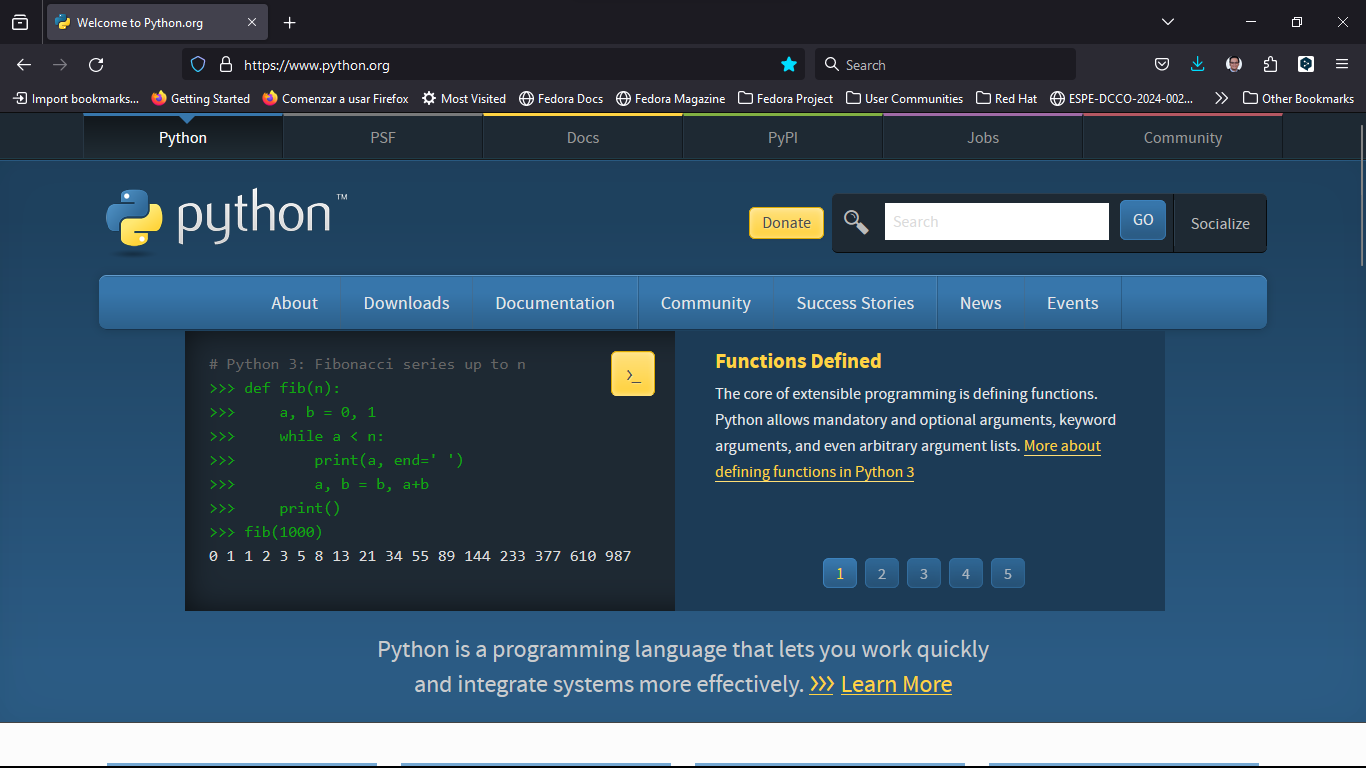
\includegraphics{unidades/unidad2/images/paste-1.png}

En la página de descargas, haga clic en el botón de descarga para la
última versión de Python. En el momento de escribir este tutorial, la
última versión de Python es 3.12.1

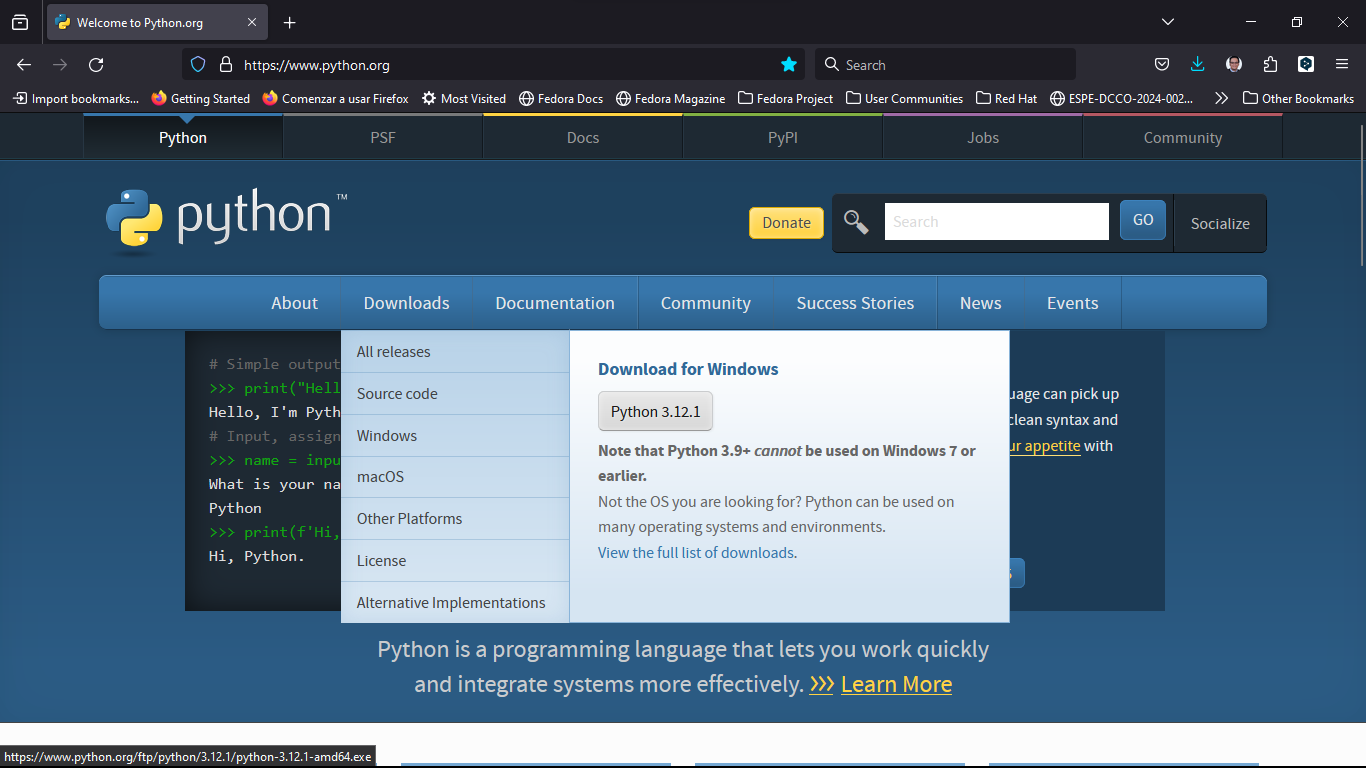
\includegraphics{unidades/unidad2/images/paste-2.png}

Excelente, ahora que hemos descargado el instalador de Python, podemos
continuar con la instalación de Python en Windows.

\begin{enumerate}
\def\labelenumi{\arabic{enumi}.}
\setcounter{enumi}{1}
\tightlist
\item
  \textbf{Instalar Python}
\end{enumerate}

Una vez que el instalador de Python se haya descargado, haga doble clic
en el archivo de instalación para iniciar el proceso de instalación.
Asegúrese de marcar la casilla que dice ``Add Python 3.12 to PATH''
antes de hacer clic en el botón ``Install Now''.


\includegraphics{unidades/unidad2/images/paste-4.png}

Ahora que hemos instalado Python en nuestra computadora, podemos
continuar con la configuración de nuestro entorno de desarrollo para
escribir y ejecutar programas en Python.

\begin{enumerate}
\def\labelenumi{\arabic{enumi}.}
\setcounter{enumi}{2}
\tightlist
\item
  \textbf{Comprobar que tenemos instalado Python}
\end{enumerate}

Para comprobar que Python se ha instalado correctamente en nuestra
computadora, abra una ventana de comandos y escriba el siguiente
comando:

\begin{Shaded}
\begin{Highlighting}[]
\ExtensionTok{python} \AttributeTok{{-}{-}version}
\end{Highlighting}
\end{Shaded}

\begin{enumerate}
\def\labelenumi{\arabic{enumi}.}
\setcounter{enumi}{3}
\tightlist
\item
  \textbf{Impresion de la versión de Python}
\end{enumerate}

Este comando imprimirá la versión de Python que está instalada en su
computadora. En mi caso, la versión de Python es 3.12.1.

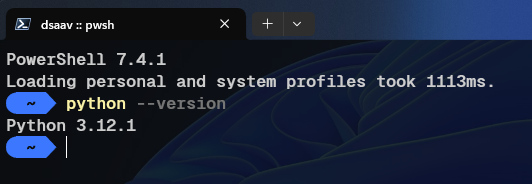
\includegraphics{unidades/unidad2/images/paste-5.png}

\subsection{Paso 3: Crear nuestro primer ``Hola Mundo'' en Python
🗺️.}\label{paso-3-crear-nuestro-primer-hola-mundo-en-python-.}

Ahora que hemos instalado Python en nuestra computadora, podemos
comenzar a escribir y ejecutar programas en Python. Para hacer esto,
necesitamos un editor de texto para escribir nuestro código y un
intérprete de Python para ejecutar nuestro código.

En este tutorial, usaremos Visual Studio Code como nuestro editor de
texto y el intérprete de Python que instalamos en el paso anterior.

\begin{enumerate}
\def\labelenumi{\arabic{enumi}.}
\tightlist
\item
  \textbf{Instalar Visual Studio Code}
\end{enumerate}

Para instalar Visual Studio Code, vaya al sitio web oficial de Visual
Studio Code en el siguiente enlace:

\url{https://code.visualstudio.com/}

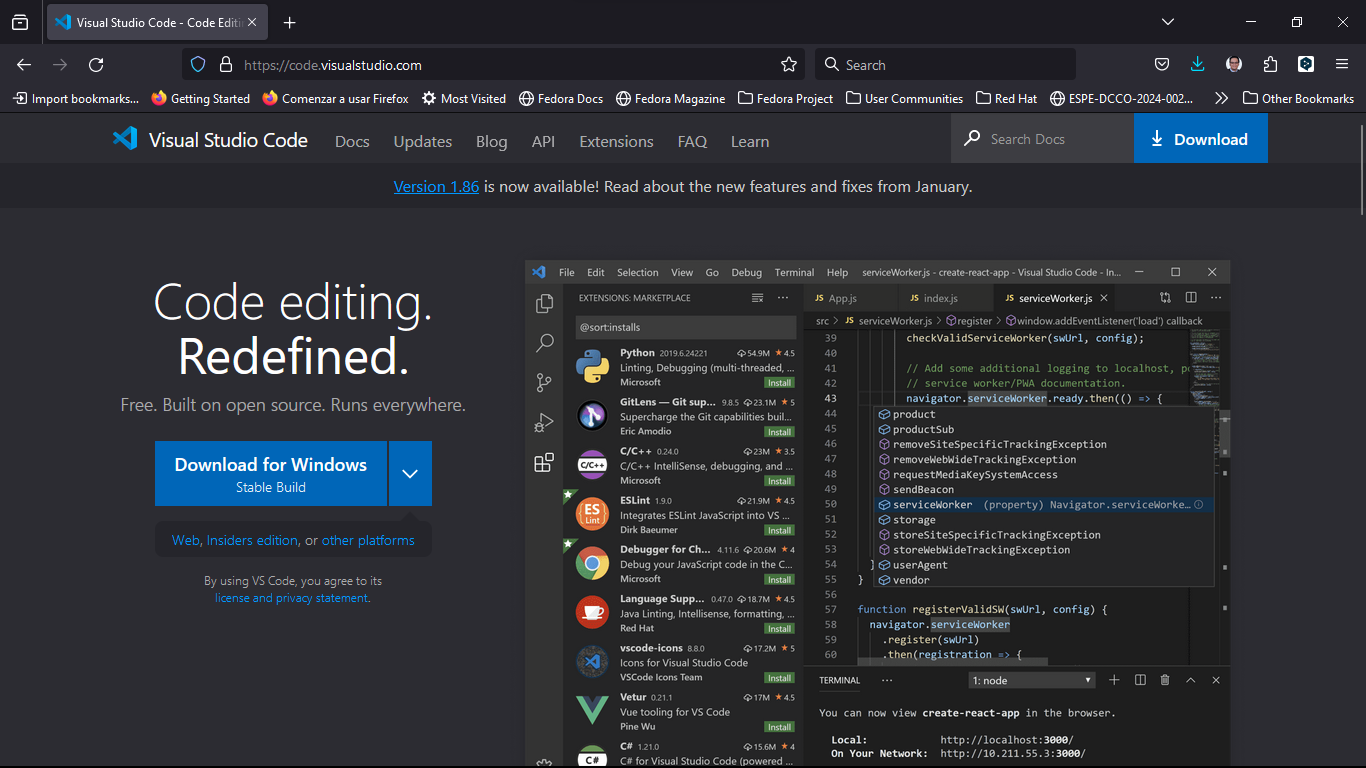
\includegraphics{unidades/unidad2/images/paste-6.png}

En la página de descargas, haga clic en el botón de descarga para su
sistema operativo. En el momento de escribir este tutorial, la última
versión de Visual Studio Code es 1.85.2.

Una vez que el instalador de Visual Studio Code se haya descargado, haga
doble clic en el archivo de instalación para iniciar el proceso de
instalación. Siga las instrucciones en pantalla para completar la
instalación.

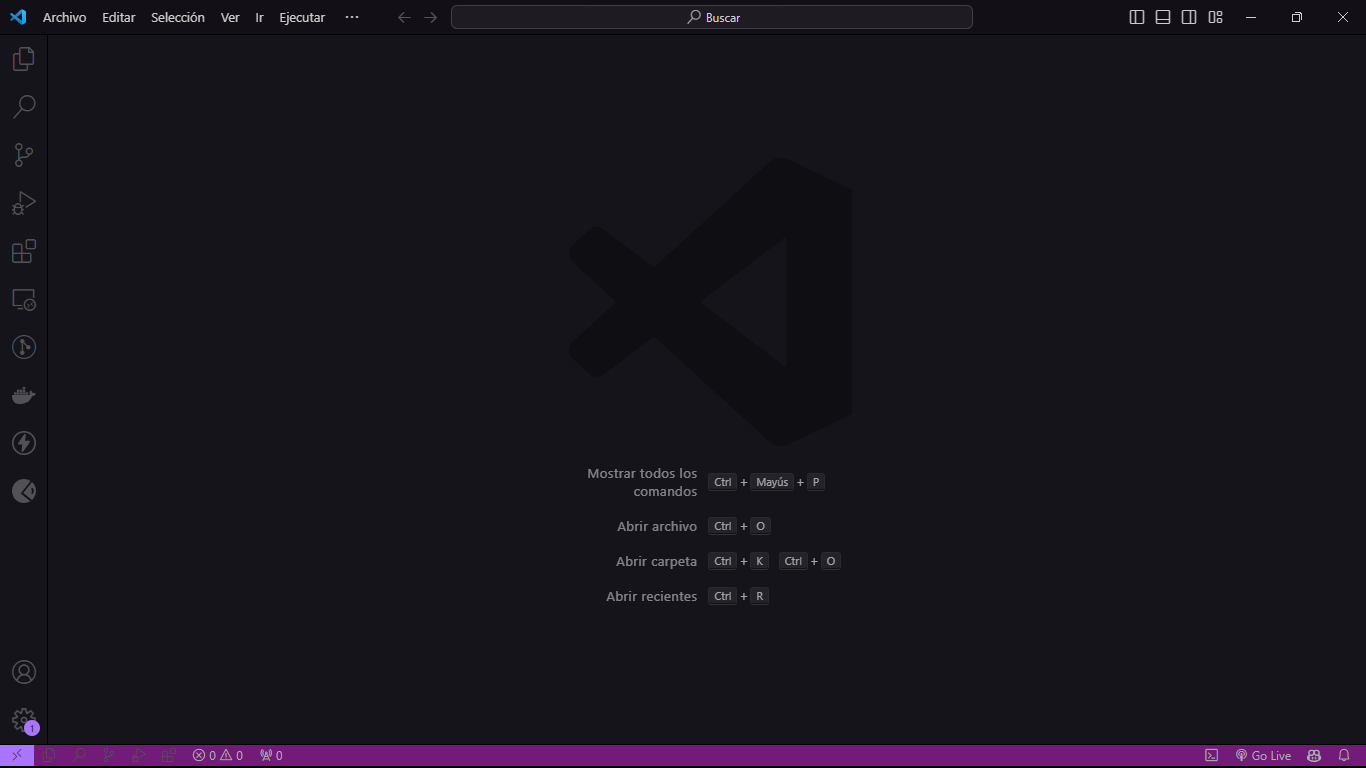
\includegraphics{unidades/unidad2/images/paste-7.png}

\begin{enumerate}
\def\labelenumi{\arabic{enumi}.}
\setcounter{enumi}{1}
\tightlist
\item
  \textbf{Crear un nuevo archivo de Python}
\end{enumerate}

Para crear un nuevo archivo de Python en Visual Studio Code, abra Visual
Studio Code y haga clic en el botón ``New File'' en la barra de
herramientas. Luego, escriba el siguiente código en el archivo:

\begin{Shaded}
\begin{Highlighting}[]
\BuiltInTok{print}\NormalTok{(}\StringTok{"Hola Mundo"}\NormalTok{)}
\end{Highlighting}
\end{Shaded}

\begin{enumerate}
\def\labelenumi{\arabic{enumi}.}
\setcounter{enumi}{2}
\tightlist
\item
  Este código imprimirá ``Hola Mundo'' en la consola.
\end{enumerate}

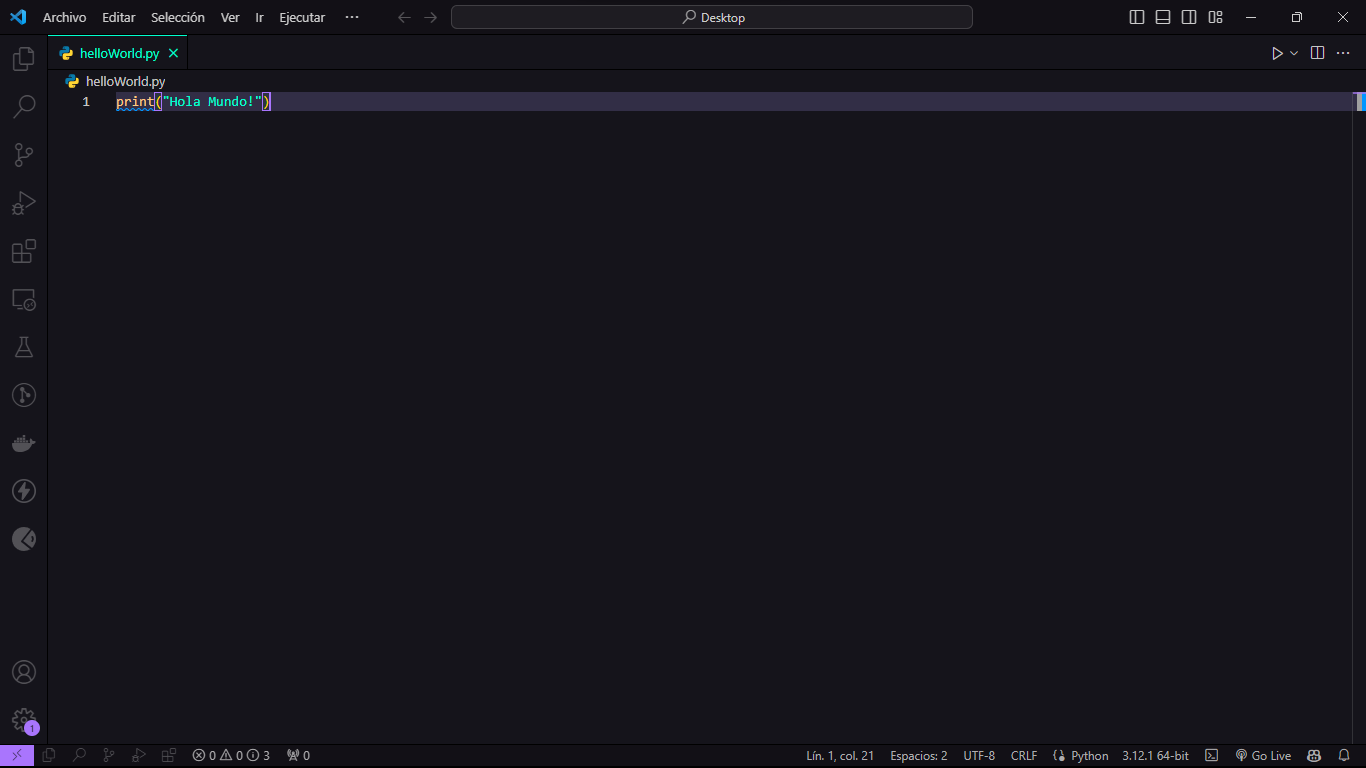
\includegraphics{unidades/unidad2/images/paste-8.png}

\begin{enumerate}
\def\labelenumi{\arabic{enumi}.}
\setcounter{enumi}{3}
\tightlist
\item
  Ejecutar el programa
\end{enumerate}

Para ejecutar el programa, haga clic en el botón ``Run'' en la barra de
herramientas. Esto ejecutará el programa y mostrará ``Hola Mundo'' en la
consola.

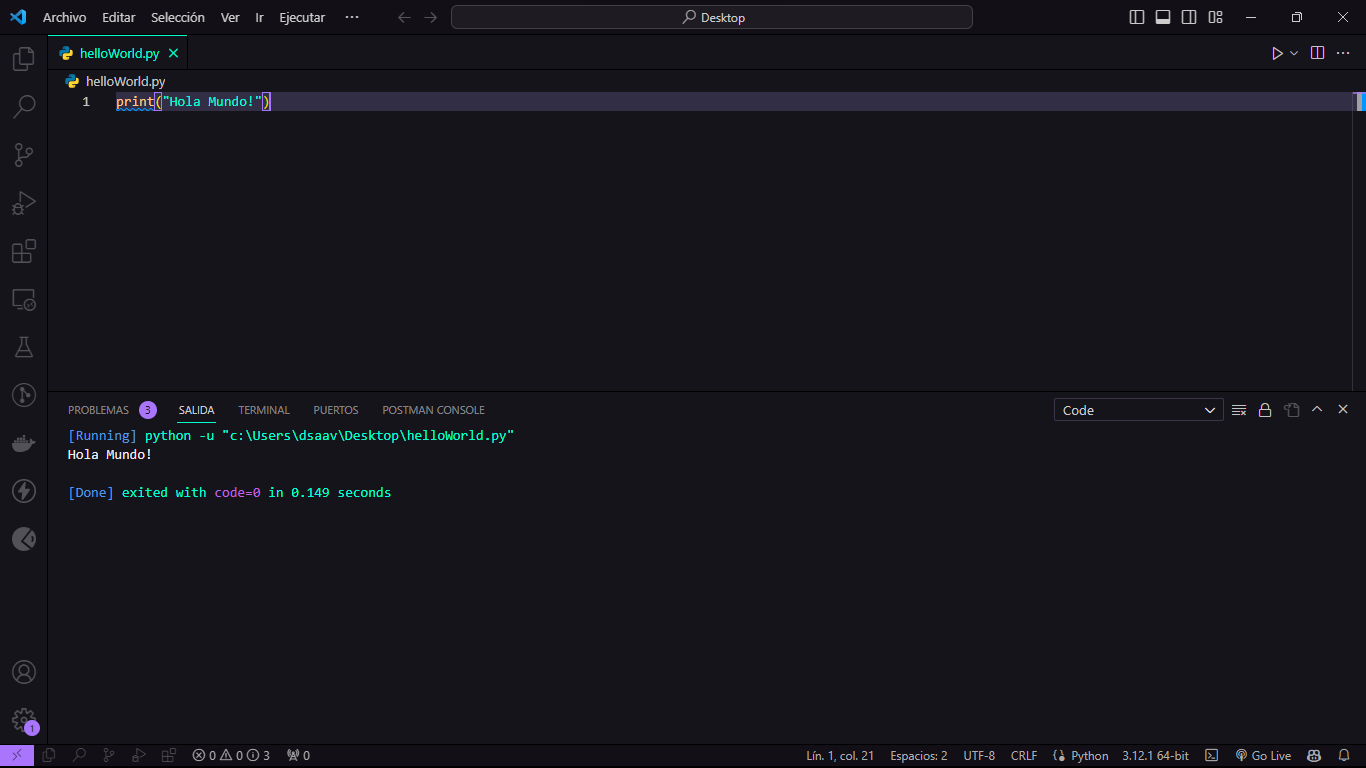
\includegraphics{unidades/unidad2/images/paste-9.png}

¡Felicidades!

Acabas de escribir y ejecutar tu primer programa en Python. Ahora que
has configurado tu entorno de desarrollo y has escrito tu primer
programa en Python, puedes comenzar a explorar el lenguaje de
programación Python y aprender a escribir programas más complejos.

\chapter{Sintaxis Básica}\label{sintaxis-buxe1sica}

\begin{figure}[H]

{\centering 
\includegraphics[width=2.08333in,height=\textheight]{unidades/unidad2/../../images/python-logo.png}

}

\caption{Python}

\end{figure}%

\phantomsection\label{annotated-cell-25}%
\begin{Shaded}
\begin{Highlighting}[]
\ControlFlowTok{if} \DecValTok{5} \OperatorTok{\textgreater{}} \DecValTok{2}\NormalTok{:}
  \BuiltInTok{print}\NormalTok{(}\StringTok{"Cinco es mayor que dos"}\NormalTok{) }\hspace*{\fill}\NormalTok{\circled{1}}
\end{Highlighting}
\end{Shaded}

\begin{description}
\tightlist
\item[\circled{1}]
En el ejemplo anterior, la instrucción \textbf{print} está indentada, es
decir, tiene un espacio al principio de la línea. Esto es necesario para
que el código funcione correctamente.
\end{description}

Además de la indentación, en python se utilizan los dos puntos
\textbf{:} para indicar que se va a escribir un bloque de código.

\phantomsection\label{annotated-cell-26}%
\begin{Shaded}
\begin{Highlighting}[]
\ControlFlowTok{if} \DecValTok{5} \OperatorTok{\textgreater{}} \DecValTok{2}\NormalTok{: }\hspace*{\fill}\NormalTok{\circled{1}}
  \BuiltInTok{print}\NormalTok{(}\StringTok{"Cinco es mayor que dos"}\NormalTok{) }
\end{Highlighting}
\end{Shaded}

\begin{description}
\tightlist
\item[\circled{1}]
En este caso, el \textbf{:} indica que se va a escribir un bloque de
código, el bloque de código que se ejecutará si la condición es
verdadera.
\end{description}

\chapter{Comentarios}\label{comentarios}

Los comentarios en python se escriben con el símbolo \textbf{\#}.

\phantomsection\label{annotated-cell-27}%
\begin{Shaded}
\begin{Highlighting}[]
\CommentTok{\# Este es un comentario}
\BuiltInTok{print}\NormalTok{(}\StringTok{"Hola Mundo"}\NormalTok{) }\hspace*{\fill}\NormalTok{\circled{1}}
\end{Highlighting}
\end{Shaded}

\begin{description}
\tightlist
\item[\circled{1}]
En este caso, el comentario está al final de la línea de código.
\end{description}

\chapter{Variables y Tipos de Datos}\label{variables-y-tipos-de-datos}

\begin{tcolorbox}[enhanced jigsaw, bottomrule=.15mm, title=\textcolor{quarto-callout-tip-color}{\faLightbulb}\hspace{0.5em}{Tip}, coltitle=black, leftrule=.75mm, left=2mm, colbacktitle=quarto-callout-tip-color!10!white, breakable, colframe=quarto-callout-tip-color-frame, colback=white, opacitybacktitle=0.6, opacityback=0, bottomtitle=1mm, toptitle=1mm, toprule=.15mm, arc=.35mm, titlerule=0mm, rightrule=.15mm]

Existe la forma de declarar variables de python con su tipo de dato

Ejemplo:

\phantomsection\label{annotated-cell-126}%
\begin{Shaded}
\begin{Highlighting}[]
\NormalTok{x: }\BuiltInTok{int} \OperatorTok{=} \DecValTok{5} \hspace*{\fill}\NormalTok{\circled{1}}
\NormalTok{y: }\BuiltInTok{str} \OperatorTok{=} \StringTok{"Hola Mundo"} \hspace*{\fill}\NormalTok{\circled{2}}
\end{Highlighting}
\end{Shaded}

\begin{description}
\tightlist
\item[\circled{1}]
En este caso, la variable \textbf{x} es de tipo entero.
\item[\circled{2}]
En este caso, la variable \textbf{y} es de tipo cadena de texto.
\end{description}

\end{tcolorbox}

En python, las variables se definen de la siguiente manera:

\phantomsection\label{annotated-cell-28}%
\begin{Shaded}
\begin{Highlighting}[]
\NormalTok{x }\OperatorTok{=} \DecValTok{5} \hspace*{\fill}\NormalTok{\circled{1}}
\NormalTok{y }\OperatorTok{=} \StringTok{"Hola Mundo"} \hspace*{\fill}\NormalTok{\circled{2}}
\end{Highlighting}
\end{Shaded}

\begin{description}
\tightlist
\item[\circled{1}]
En este caso, la variable \textbf{x} es de tipo entero.
\item[\circled{2}]
En este caso, la variable \textbf{y} es de tipo cadena de texto.
\end{description}

\chapter{Tipos de Datos}\label{tipos-de-datos}

En python, los tipos de datos más comunes son:

\begin{itemize}
\tightlist
\item
  \textbf{int}: Entero
\end{itemize}

Ejemplo:

\phantomsection\label{annotated-cell-29}%
\begin{Shaded}
\begin{Highlighting}[]
\NormalTok{x }\OperatorTok{=} \DecValTok{5} \hspace*{\fill}\NormalTok{\circled{1}}
\end{Highlighting}
\end{Shaded}

\begin{description}
\tightlist
\item[\circled{1}]
La variable \textbf{x} es de tipo entero.
\end{description}

\begin{itemize}
\tightlist
\item
  \textbf{float}: Flotante
\end{itemize}

Ejemplo:

\phantomsection\label{annotated-cell-30}%
\begin{Shaded}
\begin{Highlighting}[]
\NormalTok{y }\OperatorTok{=} \FloatTok{5.0} \hspace*{\fill}\NormalTok{\circled{1}}
\end{Highlighting}
\end{Shaded}

\begin{description}
\tightlist
\item[\circled{1}]
La variable \textbf{y} es de tipo flotante.
\end{description}

\begin{itemize}
\tightlist
\item
  \textbf{str}: Cadena de texto
\end{itemize}

Ejemplo:

\phantomsection\label{annotated-cell-31}%
\begin{Shaded}
\begin{Highlighting}[]
\NormalTok{z }\OperatorTok{=} \StringTok{"Hola Mundo"} \hspace*{\fill}\NormalTok{\circled{1}}
\end{Highlighting}
\end{Shaded}

\begin{itemize}
\tightlist
\item
  \textbf{bool}: Booleano
\end{itemize}

Ejemplo:

\phantomsection\label{annotated-cell-32}%
\begin{Shaded}
\begin{Highlighting}[]
\NormalTok{a }\OperatorTok{=} \VariableTok{True} \hspace*{\fill}\NormalTok{\circled{1}}
\end{Highlighting}
\end{Shaded}

\begin{description}
\tightlist
\item[\circled{1}]
La variable \textbf{a} es de tipo booleano.
\end{description}

\begin{itemize}
\tightlist
\item
  \textbf{list}: Lista
\end{itemize}

Ejemplo:

\phantomsection\label{annotated-cell-33}%
\begin{Shaded}
\begin{Highlighting}[]
\NormalTok{b }\OperatorTok{=}\NormalTok{ [}\DecValTok{1}\NormalTok{, }\DecValTok{2}\NormalTok{, }\DecValTok{3}\NormalTok{] }\hspace*{\fill}\NormalTok{\circled{1}}
\end{Highlighting}
\end{Shaded}

\begin{itemize}
\tightlist
\item
  \textbf{tuple}: Tupla
\end{itemize}

Ejemplo:

\phantomsection\label{annotated-cell-34}%
\begin{Shaded}
\begin{Highlighting}[]
\NormalTok{c }\OperatorTok{=}\NormalTok{ (}\DecValTok{1}\NormalTok{, }\DecValTok{2}\NormalTok{, }\DecValTok{3}\NormalTok{) }\hspace*{\fill}\NormalTok{\circled{1}}
\end{Highlighting}
\end{Shaded}

\begin{itemize}
\tightlist
\item
  \textbf{dict}: Diccionario
\end{itemize}

Ejemplo:

\phantomsection\label{annotated-cell-35}%
\begin{Shaded}
\begin{Highlighting}[]
\NormalTok{d }\OperatorTok{=}\NormalTok{ \{}\StringTok{"nombre"}\NormalTok{: }\StringTok{"Juan"}\NormalTok{, }\StringTok{"edad"}\NormalTok{: }\DecValTok{25}\NormalTok{\} }\hspace*{\fill}\NormalTok{\circled{1}}
\end{Highlighting}
\end{Shaded}

\begin{itemize}
\tightlist
\item
  \textbf{set}: Conjunto
\end{itemize}

Ejemplo:

\phantomsection\label{annotated-cell-36}%
\begin{Shaded}
\begin{Highlighting}[]
\NormalTok{e }\OperatorTok{=}\NormalTok{ \{}\DecValTok{1}\NormalTok{, }\DecValTok{2}\NormalTok{, }\DecValTok{3}\NormalTok{\} }\hspace*{\fill}\NormalTok{\circled{1}}
\end{Highlighting}
\end{Shaded}

\begin{description}
\tightlist
\item[\circled{1}]
La variable \textbf{e} es de tipo conjunto.
\end{description}

\begin{itemize}
\tightlist
\item
  \textbf{None}: Nulo
\end{itemize}

Ejemplo:

\phantomsection\label{annotated-cell-37}%
\begin{Shaded}
\begin{Highlighting}[]
\NormalTok{f }\OperatorTok{=} \VariableTok{None} \hspace*{\fill}\NormalTok{\circled{1}}
\end{Highlighting}
\end{Shaded}

\begin{description}
\tightlist
\item[\circled{1}]
La variable \textbf{f} es de tipo \textbf{None}.
\end{description}

\chapter{Operadores}\label{operadores}

En python, los operadores más comunes son:

\begin{itemize}
\tightlist
\item
  \textbf{+}: Suma
\end{itemize}

Ejemplo:

\phantomsection\label{annotated-cell-38}%
\begin{Shaded}
\begin{Highlighting}[]
\NormalTok{x }\OperatorTok{=} \DecValTok{5}
\NormalTok{y }\OperatorTok{=} \DecValTok{2}
\NormalTok{z }\OperatorTok{=}\NormalTok{ x }\OperatorTok{+}\NormalTok{ y }\hspace*{\fill}\NormalTok{\circled{1}}
\end{Highlighting}
\end{Shaded}

\begin{description}
\tightlist
\item[\circled{1}]
La variable \textbf{z} es igual a la suma de \textbf{x} y \textbf{y}.
\end{description}

\begin{itemize}
\tightlist
\item
  \textbf{-}: Resta
\end{itemize}

Ejemplo:

\phantomsection\label{annotated-cell-39}%
\begin{Shaded}
\begin{Highlighting}[]
\NormalTok{x }\OperatorTok{=} \DecValTok{5}
\NormalTok{y }\OperatorTok{=} \DecValTok{2}
\NormalTok{a }\OperatorTok{=}\NormalTok{ x }\OperatorTok{{-}}\NormalTok{ y }\hspace*{\fill}\NormalTok{\circled{1}}
\end{Highlighting}
\end{Shaded}

\begin{description}
\tightlist
\item[\circled{1}]
La variable \textbf{a} es igual a la resta de \textbf{x} y \textbf{y}.
\end{description}

\begin{itemize}
\tightlist
\item
  **``*``**: Multiplicación
\end{itemize}

Ejemplo:

\phantomsection\label{annotated-cell-40}%
\begin{Shaded}
\begin{Highlighting}[]
\NormalTok{x }\OperatorTok{=} \DecValTok{5}
\NormalTok{y }\OperatorTok{=} \DecValTok{2}
\NormalTok{b }\OperatorTok{=}\NormalTok{ x }\OperatorTok{*}\NormalTok{ y }\hspace*{\fill}\NormalTok{\circled{1}}
\end{Highlighting}
\end{Shaded}

\begin{description}
\tightlist
\item[\circled{1}]
La variable \textbf{b} es igual a la multiplicación de \textbf{x} y
\textbf{y}.
\end{description}

\begin{itemize}
\tightlist
\item
  \textbf{/}: División
\end{itemize}

Ejemplo:

\phantomsection\label{annotated-cell-41}%
\begin{Shaded}
\begin{Highlighting}[]
\NormalTok{x }\OperatorTok{=} \DecValTok{5}
\NormalTok{y }\OperatorTok{=} \DecValTok{2}
\NormalTok{c }\OperatorTok{=}\NormalTok{ x }\OperatorTok{/}\NormalTok{ y }\hspace*{\fill}\NormalTok{\circled{1}}
\end{Highlighting}
\end{Shaded}

\begin{description}
\tightlist
\item[\circled{1}]
La variable \textbf{c} es igual a la división de \textbf{x} y
\textbf{y}.
\end{description}

\begin{itemize}
\tightlist
\item
  \textbf{//}: División entera
\end{itemize}

Ejemplo:

\phantomsection\label{annotated-cell-42}%
\begin{Shaded}
\begin{Highlighting}[]
\NormalTok{x }\OperatorTok{=} \DecValTok{5}
\NormalTok{y }\OperatorTok{=} \DecValTok{2}
\NormalTok{d }\OperatorTok{=}\NormalTok{ x }\OperatorTok{//}\NormalTok{ y }\hspace*{\fill}\NormalTok{\circled{1}}
\end{Highlighting}
\end{Shaded}

\begin{description}
\tightlist
\item[\circled{1}]
La variable \textbf{d} es igual a la división entera de \textbf{x} y
\textbf{y}.
\end{description}

\begin{itemize}
\tightlist
\item
  \textbf{\%}: Módulo
\end{itemize}

Ejemplo:

\phantomsection\label{annotated-cell-43}%
\begin{Shaded}
\begin{Highlighting}[]
\NormalTok{x }\OperatorTok{=} \DecValTok{5}
\NormalTok{y }\OperatorTok{=} \DecValTok{2}
\NormalTok{e }\OperatorTok{=}\NormalTok{ x }\OperatorTok{\%}\NormalTok{ y }\hspace*{\fill}\NormalTok{\circled{1}}
\end{Highlighting}
\end{Shaded}

\begin{description}
\tightlist
\item[\circled{1}]
La variable \textbf{e} es igual al módulo de \textbf{x} y \textbf{y}.
\end{description}

\begin{itemize}
\tightlist
\item
  \textbf{``}''**: Potencia
\end{itemize}

Ejemplo:

\phantomsection\label{annotated-cell-44}%
\begin{Shaded}
\begin{Highlighting}[]
\NormalTok{x }\OperatorTok{=} \DecValTok{5}
\NormalTok{y }\OperatorTok{=} \DecValTok{2}
\NormalTok{f }\OperatorTok{=}\NormalTok{ x }\OperatorTok{**}\NormalTok{ y }\hspace*{\fill}\NormalTok{\circled{1}}
\end{Highlighting}
\end{Shaded}

\begin{description}
\tightlist
\item[\circled{1}]
La variable \textbf{f} es igual a la potencia de \textbf{x} y
\textbf{y}.
\end{description}

\begin{itemize}
\tightlist
\item
  \textbf{==}: Igualdad
\end{itemize}

Ejemplo:

\phantomsection\label{annotated-cell-45}%
\begin{Shaded}
\begin{Highlighting}[]
\NormalTok{x }\OperatorTok{=} \DecValTok{5}
\NormalTok{y }\OperatorTok{=} \DecValTok{2}
\NormalTok{g }\OperatorTok{=}\NormalTok{ x }\OperatorTok{==}\NormalTok{ y }\hspace*{\fill}\NormalTok{\circled{1}}
\end{Highlighting}
\end{Shaded}

\begin{description}
\tightlist
\item[\circled{1}]
La variable \textbf{g} es igual a la comparación de igualdad entre
\textbf{x} y \textbf{y}.
\end{description}

\begin{itemize}
\tightlist
\item
  \textbf{!=}: Diferente
\end{itemize}

Ejemplo:

\phantomsection\label{annotated-cell-46}%
\begin{Shaded}
\begin{Highlighting}[]
\NormalTok{x }\OperatorTok{=} \DecValTok{5}
\NormalTok{y }\OperatorTok{=} \DecValTok{2}
\NormalTok{h }\OperatorTok{=}\NormalTok{ x }\OperatorTok{!=}\NormalTok{ y }\hspace*{\fill}\NormalTok{\circled{1}}
\end{Highlighting}
\end{Shaded}

\begin{description}
\tightlist
\item[\circled{1}]
La variable \textbf{h} es igual a la comparación de diferencia entre
\textbf{x} y \textbf{y}.
\end{description}

\begin{itemize}
\tightlist
\item
  \textbf{\textgreater{}}: Mayor que
\end{itemize}

Ejemplo:

\phantomsection\label{annotated-cell-47}%
\begin{Shaded}
\begin{Highlighting}[]
\NormalTok{x }\OperatorTok{=} \DecValTok{5}
\NormalTok{y }\OperatorTok{=} \DecValTok{2}
\NormalTok{i }\OperatorTok{=}\NormalTok{ x }\OperatorTok{\textgreater{}}\NormalTok{ y }\hspace*{\fill}\NormalTok{\circled{1}}
\end{Highlighting}
\end{Shaded}

\begin{itemize}
\tightlist
\item
  \textbf{\textless{}}: Menor que
\end{itemize}

Ejemplo:

\phantomsection\label{annotated-cell-48}%
\begin{Shaded}
\begin{Highlighting}[]
\NormalTok{x }\OperatorTok{=} \DecValTok{5}
\NormalTok{y }\OperatorTok{=} \DecValTok{2}
\NormalTok{j }\OperatorTok{=}\NormalTok{ x }\OperatorTok{\textless{}}\NormalTok{ y }\hspace*{\fill}\NormalTok{\circled{1}}
\end{Highlighting}
\end{Shaded}

\begin{description}
\tightlist
\item[\circled{1}]
La variable \textbf{j} es igual a la comparación de menor que entre
\textbf{x} y \textbf{y}.
\end{description}

\begin{itemize}
\tightlist
\item
  \textbf{\textgreater=}: Mayor
\end{itemize}

Ejemplo:

\phantomsection\label{annotated-cell-49}%
\begin{Shaded}
\begin{Highlighting}[]
\NormalTok{x }\OperatorTok{=} \DecValTok{5}
\NormalTok{y }\OperatorTok{=} \DecValTok{2}
\NormalTok{k }\OperatorTok{=}\NormalTok{ x }\OperatorTok{\textgreater{}=}\NormalTok{ y }\hspace*{\fill}\NormalTok{\circled{1}}
\end{Highlighting}
\end{Shaded}

\begin{description}
\tightlist
\item[\circled{1}]
La variable \textbf{k} es igual a la comparación de mayor o igual que
entre \textbf{x} y \textbf{y}.
\end{description}

\begin{itemize}
\tightlist
\item
  \textbf{\textless=}: Menor
\end{itemize}

Ejemplo:

\phantomsection\label{annotated-cell-50}%
\begin{Shaded}
\begin{Highlighting}[]
\NormalTok{x }\OperatorTok{=} \DecValTok{5}
\NormalTok{y }\OperatorTok{=} \DecValTok{2}
\NormalTok{l }\OperatorTok{=}\NormalTok{ x }\OperatorTok{\textless{}=}\NormalTok{ y }\hspace*{\fill}\NormalTok{\circled{1}}
\end{Highlighting}
\end{Shaded}

\begin{description}
\tightlist
\item[\circled{1}]
La variable \textbf{l} es igual a la comparación de menor o igual que
entre \textbf{x} y \textbf{y}.
\end{description}

\begin{itemize}
\tightlist
\item
  \textbf{and}: Y
\end{itemize}

Ejemplo:

\phantomsection\label{annotated-cell-51}%
\begin{Shaded}
\begin{Highlighting}[]
\NormalTok{x }\OperatorTok{=} \DecValTok{5}
\NormalTok{y }\OperatorTok{=} \DecValTok{2}
\NormalTok{m }\OperatorTok{=}\NormalTok{ x }\KeywordTok{and}\NormalTok{ y }\hspace*{\fill}\NormalTok{\circled{1}}
\end{Highlighting}
\end{Shaded}

\begin{itemize}
\tightlist
\item
  \textbf{or}: O
\end{itemize}

Ejemplo:

\phantomsection\label{annotated-cell-52}%
\begin{Shaded}
\begin{Highlighting}[]
\NormalTok{x }\OperatorTok{=} \DecValTok{5}
\NormalTok{y }\OperatorTok{=} \DecValTok{2}
\NormalTok{n }\OperatorTok{=}\NormalTok{ x }\KeywordTok{or}\NormalTok{ y }\hspace*{\fill}\NormalTok{\circled{1}}
\end{Highlighting}
\end{Shaded}

\begin{description}
\tightlist
\item[\circled{1}]
La variable \textbf{n} es igual a la comparación lógica \textbf{or}
entre \textbf{x} y \textbf{y}.
\end{description}

\begin{itemize}
\tightlist
\item
  \textbf{not}: Negación
\end{itemize}

Ejemplo:

\phantomsection\label{annotated-cell-53}%
\begin{Shaded}
\begin{Highlighting}[]
\NormalTok{x }\OperatorTok{=} \DecValTok{5}
\NormalTok{o }\OperatorTok{=} \KeywordTok{not}\NormalTok{ x }\hspace*{\fill}\NormalTok{\circled{1}}
\end{Highlighting}
\end{Shaded}

\begin{description}
\tightlist
\item[\circled{1}]
La variable \textbf{o} es igual a la negación de \textbf{x}.
\end{description}

\chapter{Estructura de Control}\label{estructura-de-control}

En python, las estructuras de control más comunes son:

\begin{itemize}
\tightlist
\item
  \textbf{if}: Si
\end{itemize}

Ejemplo:

\phantomsection\label{annotated-cell-54}%
\begin{Shaded}
\begin{Highlighting}[]
\ControlFlowTok{if} \DecValTok{5} \OperatorTok{\textgreater{}} \DecValTok{2}\NormalTok{: }\hspace*{\fill}\NormalTok{\circled{1}}
  \BuiltInTok{print}\NormalTok{(}\StringTok{"Cinco es mayor que dos"}\NormalTok{) }\hspace*{\fill}\NormalTok{\circled{2}}
\end{Highlighting}
\end{Shaded}

\begin{description}
\tightlist
\item[\circled{1}]
En este caso, se evalúa si 5 es mayor que 2.
\item[\circled{2}]
Si la condición es verdadera, se imprime el mensaje ``Cinco es mayor que
dos''.
\end{description}

\begin{itemize}
\tightlist
\item
  \textbf{elif}: Si no
\end{itemize}

Ejemplo:

\phantomsection\label{annotated-cell-55}%
\begin{Shaded}
\begin{Highlighting}[]
\NormalTok{x }\OperatorTok{=} \DecValTok{5}
\NormalTok{y }\OperatorTok{=} \DecValTok{2}
\ControlFlowTok{if}\NormalTok{ x }\OperatorTok{\textgreater{}}\NormalTok{ y: }\hspace*{\fill}\NormalTok{\circled{1}}
  \BuiltInTok{print}\NormalTok{(}\StringTok{"X es mayor que Y"}\NormalTok{) }\hspace*{\fill}\NormalTok{\circled{2}}
\ControlFlowTok{elif}\NormalTok{ x }\OperatorTok{\textless{}}\NormalTok{ y: }\hspace*{\fill}\NormalTok{\circled{3}}
  \BuiltInTok{print}\NormalTok{(}\StringTok{"X es menor que Y"}\NormalTok{) }\hspace*{\fill}\NormalTok{\circled{4}}
\end{Highlighting}
\end{Shaded}

\begin{description}
\tightlist
\item[\circled{1}]
En este caso, se evalúa si \textbf{x} es mayor que \textbf{y}.
\item[\circled{2}]
Si la condición es verdadera, se imprime el mensaje ``X es mayor que
Y''.
\item[\circled{3}]
Si la condición anterior es falsa, se evalúa si \textbf{x} es menor que
\textbf{y}.
\item[\circled{4}]
Si la condición es verdadera, se imprime el mensaje ``X es menor que
Y''.
\end{description}

\begin{itemize}
\tightlist
\item
  \textbf{else}: Si no
\end{itemize}

Ejemplo:

\phantomsection\label{annotated-cell-56}%
\begin{Shaded}
\begin{Highlighting}[]
\NormalTok{x }\OperatorTok{=} \DecValTok{5}
\NormalTok{y }\OperatorTok{=} \DecValTok{2}
\ControlFlowTok{if}\NormalTok{ x }\OperatorTok{\textgreater{}}\NormalTok{ y: }\hspace*{\fill}\NormalTok{\circled{1}}
  \BuiltInTok{print}\NormalTok{(}\StringTok{"X es mayor que Y"}\NormalTok{) }\hspace*{\fill}\NormalTok{\circled{2}}
\ControlFlowTok{elif}\NormalTok{ x }\OperatorTok{\textless{}}\NormalTok{ y: }\hspace*{\fill}\NormalTok{\circled{3}}
  \BuiltInTok{print}\NormalTok{(}\StringTok{"X es menor que Y"}\NormalTok{) }\hspace*{\fill}\NormalTok{\circled{4}}
\ControlFlowTok{else}\NormalTok{: }\hspace*{\fill}\NormalTok{\circled{5}}
  \BuiltInTok{print}\NormalTok{(}\StringTok{"X es igual a Y"}\NormalTok{) }\hspace*{\fill}\NormalTok{\circled{6}}
\end{Highlighting}
\end{Shaded}

\begin{description}
\tightlist
\item[\circled{1}]
En este caso, se evalúa si \textbf{x} es mayor que \textbf{y}.
\item[\circled{2}]
Si la condición es verdadera, se imprime el mensaje ``X es mayor que
Y''.
\item[\circled{3}]
Si la condición anterior es falsa, se evalúa si \textbf{x} es menor que
\textbf{y}.
\item[\circled{4}]
Si la condición es verdadera, se imprime el mensaje ``X es menor que
Y''.
\item[\circled{5}]
Si las condiciones anteriores son falsas, se ejecuta el bloque de código
del \textbf{else}.
\item[\circled{6}]
En este caso, se imprime el mensaje ``X es igual a Y''.
\end{description}

\begin{itemize}
\tightlist
\item
  \textbf{for}: Para
\end{itemize}

Ejemplo:

\phantomsection\label{annotated-cell-57}%
\begin{Shaded}
\begin{Highlighting}[]
\ControlFlowTok{for}\NormalTok{ x }\KeywordTok{in} \BuiltInTok{range}\NormalTok{(}\DecValTok{5}\NormalTok{): }\hspace*{\fill}\NormalTok{\circled{1}}
  \BuiltInTok{print}\NormalTok{(x) }\hspace*{\fill}\NormalTok{\circled{2}}
\end{Highlighting}
\end{Shaded}

\begin{description}
\tightlist
\item[\circled{1}]
En este caso, se recorre un rango de 0 a 5.
\item[\circled{2}]
En cada iteración, se imprime el valor de \textbf{x}.
\end{description}

\begin{itemize}
\tightlist
\item
  \textbf{while}: Mientras
\end{itemize}

Ejemplo:

\phantomsection\label{annotated-cell-58}%
\begin{Shaded}
\begin{Highlighting}[]
\NormalTok{x }\OperatorTok{=} \DecValTok{0}
\ControlFlowTok{while}\NormalTok{ x }\OperatorTok{\textless{}} \DecValTok{5}\NormalTok{: }\hspace*{\fill}\NormalTok{\circled{1}}
  \BuiltInTok{print}\NormalTok{(x) }\hspace*{\fill}\NormalTok{\circled{2}}
\NormalTok{  x }\OperatorTok{+=} \DecValTok{1} \hspace*{\fill}\NormalTok{\circled{3}}
\end{Highlighting}
\end{Shaded}

\begin{description}
\tightlist
\item[\circled{1}]
En este caso, se evalúa si \textbf{x} es menor que 5.
\item[\circled{2}]
En cada iteración, se imprime el valor de \textbf{x}.
\item[\circled{3}]
En cada iteración, se incrementa el valor de \textbf{x}.
\end{description}

\begin{itemize}
\tightlist
\item
  \textbf{break}: Romper
\end{itemize}

Ejemplo:

\phantomsection\label{annotated-cell-59}%
\begin{Shaded}
\begin{Highlighting}[]
\NormalTok{x }\OperatorTok{=} \DecValTok{0}
\ControlFlowTok{while}\NormalTok{ x }\OperatorTok{\textless{}} \DecValTok{5}\NormalTok{: }\hspace*{\fill}\NormalTok{\circled{1}}
  \BuiltInTok{print}\NormalTok{(x) }\hspace*{\fill}\NormalTok{\circled{2}}
\NormalTok{  x }\OperatorTok{+=} \DecValTok{1} \hspace*{\fill}\NormalTok{\circled{3}}
  \ControlFlowTok{if}\NormalTok{ x }\OperatorTok{==} \DecValTok{3}\NormalTok{: }\hspace*{\fill}\NormalTok{\circled{4}}
    \ControlFlowTok{break} \hspace*{\fill}\NormalTok{\circled{5}}
\end{Highlighting}
\end{Shaded}

\begin{description}
\tightlist
\item[\circled{1}]
En este caso, se evalúa si \textbf{x} es menor que 5.
\item[\circled{2}]
En cada iteración, se imprime el valor de \textbf{x}.
\item[\circled{3}]
En cada iteración, se incrementa el valor de \textbf{x}.
\item[\circled{4}]
En cada iteración, se evalúa si \textbf{x} es igual a 3.
\item[\circled{5}]
Si la condición es verdadera, se rompe el ciclo.
\end{description}

\begin{itemize}
\tightlist
\item
  \textbf{continue}: Continuar
\end{itemize}

Ejemplo:

\phantomsection\label{annotated-cell-60}%
\begin{Shaded}
\begin{Highlighting}[]
\NormalTok{x }\OperatorTok{=} \DecValTok{0}
\ControlFlowTok{while}\NormalTok{ x }\OperatorTok{\textless{}} \DecValTok{5}\NormalTok{: }\hspace*{\fill}\NormalTok{\circled{1}}
\NormalTok{  x }\OperatorTok{+=} \DecValTok{1} \hspace*{\fill}\NormalTok{\circled{2}}
  \ControlFlowTok{if}\NormalTok{ x }\OperatorTok{==} \DecValTok{3}\NormalTok{: }\hspace*{\fill}\NormalTok{\circled{3}}
    \ControlFlowTok{continue} \hspace*{\fill}\NormalTok{\circled{4}}
  \BuiltInTok{print}\NormalTok{(x) }\hspace*{\fill}\NormalTok{\circled{5}}
\end{Highlighting}
\end{Shaded}

\begin{description}
\tightlist
\item[\circled{1}]
En este caso, se evalúa si \textbf{x} es menor que 5.
\item[\circled{2}]
En cada iteración, se incrementa el valor de \textbf{x}.
\item[\circled{3}]
En cada iteración, se evalúa si \textbf{x} es igual a 3.
\item[\circled{4}]
Si la condición es verdadera, se continúa con la siguiente iteración.
\item[\circled{5}]
En cada iteración, se imprime el valor de \textbf{x}.
\end{description}

\begin{itemize}
\tightlist
\item
  \textbf{pass}: Pasar
\end{itemize}

Ejemplo:

\phantomsection\label{annotated-cell-61}%
\begin{Shaded}
\begin{Highlighting}[]
\NormalTok{x }\OperatorTok{=} \DecValTok{0}
\ControlFlowTok{if}\NormalTok{ x }\OperatorTok{==} \DecValTok{0}\NormalTok{: }\hspace*{\fill}\NormalTok{\circled{1}}
  \ControlFlowTok{pass} \hspace*{\fill}\NormalTok{\circled{2}}
\end{Highlighting}
\end{Shaded}

\begin{description}
\tightlist
\item[\circled{1}]
En este caso, se evalúa si \textbf{x} es igual a 0.
\item[\circled{2}]
Si la condición es verdadera, no se hace nada.
\end{description}

\begin{itemize}
\tightlist
\item
  \textbf{return}: Retornar
\end{itemize}

Ejemplo:

\phantomsection\label{annotated-cell-62}%
\begin{Shaded}
\begin{Highlighting}[]
\KeywordTok{def}\NormalTok{ suma(x, y): }\hspace*{\fill}\NormalTok{\circled{1}}
  \ControlFlowTok{return}\NormalTok{ x }\OperatorTok{+}\NormalTok{ y }\hspace*{\fill}\NormalTok{\circled{2}}
\end{Highlighting}
\end{Shaded}

\begin{description}
\tightlist
\item[\circled{1}]
En este caso, se define una función llamada \textbf{suma} que recibe dos
parámetros \textbf{x} y \textbf{y}.
\item[\circled{2}]
La función retorna la suma de \textbf{x} y \textbf{y}.
\end{description}

\begin{itemize}
\tightlist
\item
  \textbf{def}: Definir
\end{itemize}

Ejemplo:

\phantomsection\label{annotated-cell-63}%
\begin{Shaded}
\begin{Highlighting}[]
\KeywordTok{def}\NormalTok{ suma(x, y): }\hspace*{\fill}\NormalTok{\circled{1}}
  \ControlFlowTok{return}\NormalTok{ x }\OperatorTok{+}\NormalTok{ y }\hspace*{\fill}\NormalTok{\circled{2}}
\end{Highlighting}
\end{Shaded}

\begin{description}
\tightlist
\item[\circled{1}]
En este caso, se define una función llamada \textbf{suma} que recibe dos
parámetros \textbf{x} y \textbf{y}.
\item[\circled{2}]
La función retorna la suma de \textbf{x} y \textbf{y}.
\end{description}

\begin{itemize}
\tightlist
\item
  \textbf{try}: Intentar
\end{itemize}

Ejemplo:

\phantomsection\label{annotated-cell-64}%
\begin{Shaded}
\begin{Highlighting}[]
\ControlFlowTok{try}\NormalTok{: }\hspace*{\fill}\NormalTok{\circled{1}}
  \BuiltInTok{print}\NormalTok{(x) }\hspace*{\fill}\NormalTok{\circled{2}}
\ControlFlowTok{except}\NormalTok{: }\hspace*{\fill}\NormalTok{\circled{3}}
  \BuiltInTok{print}\NormalTok{(}\StringTok{"Ocurrió un error"}\NormalTok{) }\hspace*{\fill}\NormalTok{\circled{4}}
\end{Highlighting}
\end{Shaded}

\begin{description}
\tightlist
\item[\circled{1}]
En este caso, se intenta ejecutar el bloque de código.
\item[\circled{2}]
Si ocurre un error, se ejecuta el bloque de código del \textbf{except}.
\item[\circled{3}]
En este caso, se imprime el mensaje ``Ocurrió un error''.
\item[\circled{4}]
Si no ocurre un error, se continúa con la ejecución del código.
\end{description}

\begin{itemize}
\tightlist
\item
  \textbf{except}: Excepto
\end{itemize}

Ejemplo:

\phantomsection\label{annotated-cell-65}%
\begin{Shaded}
\begin{Highlighting}[]
\ControlFlowTok{try}\NormalTok{: }\hspace*{\fill}\NormalTok{\circled{1}}
  \BuiltInTok{print}\NormalTok{(x) }\hspace*{\fill}\NormalTok{\circled{2}}
\ControlFlowTok{except}\NormalTok{: }\hspace*{\fill}\NormalTok{\circled{3}}
  \BuiltInTok{print}\NormalTok{(}\StringTok{"Ocurrió un error"}\NormalTok{) }\hspace*{\fill}\NormalTok{\circled{4}}
\end{Highlighting}
\end{Shaded}

\begin{description}
\tightlist
\item[\circled{1}]
En este caso, se intenta ejecutar el bloque de código.
\item[\circled{2}]
Si ocurre un error, se ejecuta el bloque de código del \textbf{except}.
\item[\circled{3}]
En este caso, se imprime el mensaje ``Ocurrió un error''.
\item[\circled{4}]
Si no ocurre un error, se continúa con la ejecución del código.
\end{description}

\begin{itemize}
\tightlist
\item
  \textbf{finally}: Finalmente
\end{itemize}

Ejemplo:

\phantomsection\label{annotated-cell-66}%
\begin{Shaded}
\begin{Highlighting}[]
\ControlFlowTok{try}\NormalTok{: }\hspace*{\fill}\NormalTok{\circled{1}}
  \BuiltInTok{print}\NormalTok{(x) }\hspace*{\fill}\NormalTok{\circled{2}}
\ControlFlowTok{except}\NormalTok{: }\hspace*{\fill}\NormalTok{\circled{3}}
  \BuiltInTok{print}\NormalTok{(}\StringTok{"Ocurrió un error"}\NormalTok{) }\hspace*{\fill}\NormalTok{\circled{4}}
\ControlFlowTok{finally}\NormalTok{: }\hspace*{\fill}\NormalTok{\circled{5}}
  \BuiltInTok{print}\NormalTok{(}\StringTok{"Finalizó la ejecución"}\NormalTok{) }\hspace*{\fill}\NormalTok{\circled{6}}
\end{Highlighting}
\end{Shaded}

\begin{description}
\tightlist
\item[\circled{1}]
En este caso, se intenta ejecutar el bloque de código.
\item[\circled{2}]
Si ocurre un error, se ejecuta el bloque de código del \texttt{except}.
\item[\circled{3}]
En este caso, se imprime el mensaje ``Ocurrió un error''.
\item[\circled{4}]
Si no ocurre un error, se continúa con la ejecución del código.
\item[\circled{5}]
Al finalizar la ejecución del bloque de código, se ejecuta el bloque de
código del \texttt{finally}.
\item[\circled{6}]
En este caso, se imprime el mensaje ``Finalizó la ejecución''.
\end{description}

\begin{itemize}
\tightlist
\item
  \textbf{raise}: Lanzar
\end{itemize}

Ejemplo:

\phantomsection\label{annotated-cell-67}%
\begin{Shaded}
\begin{Highlighting}[]
\ControlFlowTok{if}\NormalTok{ x }\OperatorTok{\textless{}} \DecValTok{0}\NormalTok{: }\hspace*{\fill}\NormalTok{\circled{1}}
  \ControlFlowTok{raise} \PreprocessorTok{Exception}\NormalTok{(}\StringTok{"El número no puede ser negativo"}\NormalTok{) }\hspace*{\fill}\NormalTok{\circled{2}}
\end{Highlighting}
\end{Shaded}

\begin{description}
\tightlist
\item[\circled{1}]
En este caso, se evalúa si \texttt{x} es menor que 0.
\item[\circled{2}]
Si la condición es verdadera, se lanza una excepción con el mensaje ``El
número no puede ser negativo''.
\end{description}

\begin{itemize}
\tightlist
\item
  \textbf{assert}: Afirmar
\end{itemize}

Ejemplo:

\phantomsection\label{annotated-cell-68}%
\begin{Shaded}
\begin{Highlighting}[]
\ControlFlowTok{assert}\NormalTok{ x }\OperatorTok{\textgreater{}} \DecValTok{0}\NormalTok{, }\StringTok{"El número no puede ser negativo"} \hspace*{\fill}\NormalTok{\circled{1}}
\end{Highlighting}
\end{Shaded}

\begin{description}
\tightlist
\item[\circled{1}]
En este caso, se evalúa si \texttt{x} es mayor que 0.
\end{description}

\begin{itemize}
\tightlist
\item
  \textbf{import}: Importar
\end{itemize}

Ejemplo:

\phantomsection\label{annotated-cell-69}%
\begin{Shaded}
\begin{Highlighting}[]
\ImportTok{import}\NormalTok{ math }\hspace*{\fill}\NormalTok{\circled{1}}
\end{Highlighting}
\end{Shaded}

\begin{description}
\tightlist
\item[\circled{1}]
En este caso, se importa el módulo \textbf{math}.
\end{description}

\begin{itemize}
\tightlist
\item
  \textbf{from}: Desde
\end{itemize}

Ejemplo:

\phantomsection\label{annotated-cell-70}%
\begin{Shaded}
\begin{Highlighting}[]
\ImportTok{from}\NormalTok{ math }\ImportTok{import}\NormalTok{ sqrt }\hspace*{\fill}\NormalTok{\circled{1}}
\end{Highlighting}
\end{Shaded}

\begin{description}
\tightlist
\item[\circled{1}]
En este caso, se importa la función \textbf{sqrt} del módulo
\textbf{math}.
\end{description}

\begin{itemize}
\tightlist
\item
  \textbf{as}: Como
\end{itemize}

Ejemplo:

\phantomsection\label{annotated-cell-71}%
\begin{Shaded}
\begin{Highlighting}[]
\ImportTok{import}\NormalTok{ math }\ImportTok{as}\NormalTok{ m }\hspace*{\fill}\NormalTok{\circled{1}}
\end{Highlighting}
\end{Shaded}

\begin{description}
\tightlist
\item[\circled{1}]
En este caso, se importa el módulo \textbf{math} como \textbf{m}.
\end{description}

\chapter{Funciones}\label{funciones}

En python, las funciones se definen de la siguiente manera:

\phantomsection\label{annotated-cell-72}%
\begin{Shaded}
\begin{Highlighting}[]
\KeywordTok{def}\NormalTok{ suma(x, y): }\hspace*{\fill}\NormalTok{\circled{1}}
  \ControlFlowTok{return}\NormalTok{ x }\OperatorTok{+}\NormalTok{ y }\hspace*{\fill}\NormalTok{\circled{2}}
\end{Highlighting}
\end{Shaded}

\begin{description}
\tightlist
\item[\circled{1}]
En este caso, se define una función llamada \textbf{suma} que recibe dos
parámetros \textbf{x} y \textbf{y}.
\item[\circled{2}]
La función retorna la suma de \textbf{x} y \textbf{y}.
\end{description}

\chapter{Llamada a Funciones}\label{llamada-a-funciones}

En python, las funciones se llaman de la siguiente manera:

\phantomsection\label{annotated-cell-73}%
\begin{Shaded}
\begin{Highlighting}[]
\NormalTok{z }\OperatorTok{=}\NormalTok{ suma(}\DecValTok{5}\NormalTok{, }\DecValTok{2}\NormalTok{) }\hspace*{\fill}\NormalTok{\circled{1}}
\end{Highlighting}
\end{Shaded}

\begin{description}
\tightlist
\item[\circled{1}]
En este caso, se llama a la función \textbf{suma} con los argumentos
\textbf{5} y \textbf{2}.
\end{description}

\chapter{Parámetros y Argumentos}\label{paruxe1metros-y-argumentos}

En python, los parámetros y argumentos se definen de la siguiente
manera:

\phantomsection\label{annotated-cell-74}%
\begin{Shaded}
\begin{Highlighting}[]
\KeywordTok{def}\NormalTok{ suma(x, y): }\hspace*{\fill}\NormalTok{\circled{1}}
  \ControlFlowTok{return}\NormalTok{ x }\OperatorTok{+}\NormalTok{ y }\hspace*{\fill}\NormalTok{\circled{2}}

\NormalTok{z }\OperatorTok{=}\NormalTok{ suma(}\DecValTok{5}\NormalTok{, }\DecValTok{2}\NormalTok{) }\hspace*{\fill}\NormalTok{\circled{3}}
\end{Highlighting}
\end{Shaded}

\begin{description}
\tightlist
\item[\circled{1}]
En este caso, se define una función llamada \textbf{suma} que recibe dos
parámetros \textbf{x} y \textbf{y}.
\item[\circled{2}]
La función retorna la suma de \textbf{x} y \textbf{y}.
\item[\circled{3}]
En este caso, se llama a la función \textbf{suma} con los argumentos
\textbf{5} y \textbf{2}.
\end{description}

\chapter{Retorno}\label{retorno}

En python, el retorno se realiza de la siguiente manera:

\phantomsection\label{annotated-cell-75}%
\begin{Shaded}
\begin{Highlighting}[]
\KeywordTok{def}\NormalTok{ suma(x, y): }\hspace*{\fill}\NormalTok{\circled{1}}
  \ControlFlowTok{return}\NormalTok{ x }\OperatorTok{+}\NormalTok{ y }\hspace*{\fill}\NormalTok{\circled{2}}

\NormalTok{z }\OperatorTok{=}\NormalTok{ suma(}\DecValTok{5}\NormalTok{, }\DecValTok{2}\NormalTok{) }\hspace*{\fill}\NormalTok{\circled{3}}
\end{Highlighting}
\end{Shaded}

\begin{description}
\tightlist
\item[\circled{1}]
En este caso, se define una función llamada \textbf{suma} que recibe dos
parámetros \textbf{x} y \textbf{y}.
\item[\circled{2}]
La función retorna la suma de \textbf{x} y \textbf{y}.
\item[\circled{3}]
En este caso, se llama a la función \textbf{suma} con los argumentos
\textbf{5} y \textbf{2}.
\end{description}

\chapter{Ejemplo}\label{ejemplo}

El programa \textbf{Calculadora de propinas} es un ejemplo práctico que
permite calcular la propina a dejar en un restaurante.

El funcionamiento del programa es el siguiente:

\begin{enumerate}
\def\labelenumi{\arabic{enumi}.}
\tightlist
\item
  El usuario ingresa el monto total de la cuenta del restaurante.
\item
  Luego, el usuario selecciona el porcentaje de propina que desea dejar.
  Por ejemplo, puede elegir un 10\%, 15\% o 20\%.
\item
  El programa calcula la cantidad de propina a partir del monto total de
  la cuenta y el porcentaje seleccionado.
\item
  Finalmente, el programa muestra al usuario el monto total de la
  cuenta, la cantidad de propina a dejar y el monto total a pagar (suma
  del monto total de la cuenta y la propina).
\end{enumerate}

Este programa es útil para aquellos que deseen calcular rápidamente la
cantidad de propina a dejar en un restaurante, sin tener que hacer los
cálculos manualmente. Además, puede ser una buena práctica para
familiarizarse con el uso de variables y el control de flujo en la
programación.

Ver Código

\phantomsection\label{annotated-cell-76}%
\begin{Shaded}
\begin{Highlighting}[]
\CommentTok{\# Ejemplo práctico: Calculadora de propinas}

\KeywordTok{def}\NormalTok{ calcular\_propina(total, porcentaje): }\hspace*{\fill}\NormalTok{\circled{1}}
\NormalTok{    propina }\OperatorTok{=}\NormalTok{ total }\OperatorTok{*}\NormalTok{ (porcentaje }\OperatorTok{/} \DecValTok{100}\NormalTok{) }\hspace*{\fill}\NormalTok{\circled{2}}
    \ControlFlowTok{return}\NormalTok{ propina }\hspace*{\fill}\NormalTok{\circled{3}}

\KeywordTok{def}\NormalTok{ calcular\_total\_con\_propina(total, porcentaje):}
\NormalTok{    propina }\OperatorTok{=}\NormalTok{ calcular\_propina(total, porcentaje)}
\NormalTok{    total\_con\_propina }\OperatorTok{=}\NormalTok{ total }\OperatorTok{+}\NormalTok{ propina}
    \ControlFlowTok{return}\NormalTok{ total\_con\_propina}

\KeywordTok{def}\NormalTok{ main(): }\hspace*{\fill}\NormalTok{\circled{4}}
    \BuiltInTok{print}\NormalTok{(}\StringTok{"Bienvenido a la calculadora de propinas"}\NormalTok{) }\hspace*{\fill}\NormalTok{\circled{5}}
\NormalTok{    total }\OperatorTok{=} \BuiltInTok{float}\NormalTok{(}\BuiltInTok{input}\NormalTok{(}\StringTok{"Ingrese el total de la cuenta: "}\NormalTok{)) }\hspace*{\fill}\NormalTok{\circled{6}}
\NormalTok{    porcentaje }\OperatorTok{=} \BuiltInTok{float}\NormalTok{(}\BuiltInTok{input}\NormalTok{(}\StringTok{"Ingrese el porcentaje de propina que desea dejar: "}\NormalTok{)) }\hspace*{\fill}\NormalTok{\circled{7}}
    
\NormalTok{    propina }\OperatorTok{=}\NormalTok{ calcular\_propina(total, porcentaje) }\hspace*{\fill}\NormalTok{\circled{8}}
\NormalTok{    total\_con\_propina }\OperatorTok{=}\NormalTok{ calcular\_total\_con\_propina(total, porcentaje) }\hspace*{\fill}\NormalTok{\circled{9}}
    
    \BuiltInTok{print}\NormalTok{(}\SpecialStringTok{f"La propina a dejar es: }\SpecialCharTok{\{}\NormalTok{propina}\SpecialCharTok{\}}\SpecialStringTok{"}\NormalTok{) }\hspace*{\fill}\NormalTok{\circled{10}}
    \BuiltInTok{print}\NormalTok{(}\SpecialStringTok{f"El total con propina es: }\SpecialCharTok{\{}\NormalTok{total\_con\_propina}\SpecialCharTok{\}}\SpecialStringTok{"}\NormalTok{) }\hspace*{\fill}\NormalTok{\circled{11}}

\ControlFlowTok{if} \VariableTok{\_\_name\_\_} \OperatorTok{==} \StringTok{"\_\_main\_\_"}\NormalTok{: }\hspace*{\fill}\NormalTok{\circled{12}}
\NormalTok{    main() }\hspace*{\fill}\NormalTok{\circled{13}}
\end{Highlighting}
\end{Shaded}

\begin{description}
\tightlist
\item[\circled{1}]
En este caso, se define una función llamada \textbf{calcular\_propina}
que recibe dos parámetros \textbf{total} y \textbf{porcentaje}.
\item[\circled{2}]
La función calcula la propina a partir del total y el porcentaje.
\item[\circled{3}]
La función retorna la propina.
\item[\circled{4}]
En este caso, se define una función llamada \textbf{main}.
\item[\circled{5}]
Se imprime un mensaje de bienvenida.
\item[\circled{6}]
Se solicita al usuario que ingrese el total de la cuenta.
\item[\circled{7}]
Se solicita al usuario que ingrese el porcentaje de propina que desea
dejar.
\item[\circled{8}]
Se calcula la propina a partir del total y el porcentaje.
\item[\circled{9}]
Se calcula el total con propina.
\item[\circled{10}]
Se imprime la propina a dejar.
\item[\circled{11}]
Se imprime el total con propina.
\end{description}

\chapter{Asignación}\label{asignaciuxf3n-1}

A continuación se sugiere realizar los siguientes ejercicios para
practicar la sintaxis y estructura de Python.

\href{https://classroom.github.com/a/LtHIKsxr}{Ejercicios Python Básico}

\section{Objetivo}\label{objetivo}

El objetivo de este repositorio es proporcionar una serie de ejercicios
de Python básico para que los principiantes en Python puedan practicar y
adquirir experiencia en la sintaxis y estructura de Python.

\section{¿Qué debes hacer?}\label{quuxe9-debes-hacer}

Debes Completar cada uno de los ejercicios propuetos a continuación cada
uno en su respectivo archivo, el objetivo es adquirir práctica en la
sintaxis y estructura de Python. Ejercicios

\begin{itemize}
\tightlist
\item
  \textbf{Imprimir Nombre:} Un programa simple que imprime tu nombre en
  la pantalla.
\item
  \textbf{Suma de los Números del 1 al 10:} Un programa que calcula la
  suma de los números del 1 al 10.
\item
  \textbf{Datos Personales:} Un programa que almacena tu edad, nombre y
  estatura en variables y las imprime en pantalla.
\item
  \textbf{Par o Impar:} Un programa que determina si un número ingresado
  por el usuario es par o impar.
\item
  \textbf{Área de un Círculo:} Una función que calcula el área de un
  círculo dado su radio.
\item
  \textbf{Suma de Dos Números:} Una función que recibe dos números como
  argumentos y devuelve su suma.
\item
  \textbf{Área de un Círculo con Parámetro:} Modificación de la función
  de área de un círculo para recibir el radio como parámetro.
\item
  \textbf{Conversión de Temperatura:} Un programa que convierte grados
  Celsius a Fahrenheit y viceversa.
\end{itemize}

\section{Pruebas}\label{pruebas}

Cada ejercicio tiene su archivo de prueba en el que se utilizan las
aserciones de pytest para verificar su correcto funcionamiento. Si por
ejemplo quiero aplicar el test del primer ejercicio debo completar el
primer ejercicio y comentar los demás, luego ejecutar el comando pytest
test\_1.py para verificar que el programa funciona correctamente, luego
continuar con cada uno de ellos e ir aplicando los test, hasta que al
final todos los test pasen y completar la tarea

\section{Ejecución}\label{ejecuciuxf3n}

Para ejecutar cada programa, simplemente ejecute el archivo
\textbf{programa.py}. Los archivos de prueba se pueden ejecutar con el
comando \textbf{pytest}.

\part{Unidad 3: Python Intermedio}

\chapter{Listas}\label{listas}

Las listas son un tipo de dato que nos permite almacenar diferentes
valores, en una sola variable.

\begin{itemize}
\tightlist
\item
  Las listas \textbf{son mutables}, es decir, podemos modificar su
  contenido.
\end{itemize}

Ejemplo:

\begin{Shaded}
\begin{Highlighting}[]
\NormalTok{mi\_lista }\OperatorTok{=}\NormalTok{ [}\DecValTok{1}\NormalTok{, }\DecValTok{2}\NormalTok{, }\DecValTok{3}\NormalTok{, }\DecValTok{4}\NormalTok{, }\DecValTok{5}\NormalTok{]}
\end{Highlighting}
\end{Shaded}

Ejercicio:

Crear una lista con los números del 1 al 10, y mostrarla en pantalla.

Solución

\begin{Shaded}
\begin{Highlighting}[]
\NormalTok{  mi\_lista }\OperatorTok{=}\NormalTok{ [}\DecValTok{1}\NormalTok{, }\DecValTok{2}\NormalTok{, }\DecValTok{3}\NormalTok{, }\DecValTok{4}\NormalTok{, }\DecValTok{5}\NormalTok{, }\DecValTok{6}\NormalTok{, }\DecValTok{7}\NormalTok{, }\DecValTok{8}\NormalTok{, }\DecValTok{9}\NormalTok{, }\DecValTok{10}\NormalTok{]}
  \BuiltInTok{print}\NormalTok{(mi\_lista)}
\end{Highlighting}
\end{Shaded}

\chapter{Tuplas}\label{tuplas}

Las tuplas son un tipo de dato que nos permite almacenar diferentes
valores, en una sola variable.

\begin{itemize}
\tightlist
\item
  Las tuplas \textbf{son inmutables}, es decir, no podemos modificar su
  contenido.
\end{itemize}

Ejemplo:

\begin{Shaded}
\begin{Highlighting}[]
\NormalTok{mi\_tupla }\OperatorTok{=}\NormalTok{ (}\DecValTok{1}\NormalTok{, }\DecValTok{2}\NormalTok{, }\DecValTok{3}\NormalTok{, }\DecValTok{4}\NormalTok{, }\DecValTok{5}\NormalTok{)}
\end{Highlighting}
\end{Shaded}

Ejercicio:

Crear una tupla con los números del 1 al 10, y mostrarla en pantalla.

Solución

\begin{Shaded}
\begin{Highlighting}[]
\NormalTok{  mi\_tupla }\OperatorTok{=}\NormalTok{ (}\DecValTok{1}\NormalTok{, }\DecValTok{2}\NormalTok{, }\DecValTok{3}\NormalTok{, }\DecValTok{4}\NormalTok{, }\DecValTok{5}\NormalTok{, }\DecValTok{6}\NormalTok{, }\DecValTok{7}\NormalTok{, }\DecValTok{8}\NormalTok{, }\DecValTok{9}\NormalTok{, }\DecValTok{10}\NormalTok{)}
  \BuiltInTok{print}\NormalTok{(mi\_tupla)}
\end{Highlighting}
\end{Shaded}

\chapter{Manipulación de Listas y
Tuplas}\label{manipulaciuxf3n-de-listas-y-tuplas}

Para modificar una \textbf{lista} se puede realizar diferentes
operaciones, como agregar, eliminar, modificar, y acceder a los
elementos de la lista o tupla.

Ejemplo:

\phantomsection\label{annotated-cell-81}%
\begin{Shaded}
\begin{Highlighting}[]
\NormalTok{mi\_lista }\OperatorTok{=}\NormalTok{ [}\DecValTok{1}\NormalTok{, }\DecValTok{2}\NormalTok{, }\DecValTok{3}\NormalTok{, }\DecValTok{4}\NormalTok{, }\DecValTok{5}\NormalTok{] }\hspace*{\fill}\NormalTok{\circled{1}}
\NormalTok{mi\_lista.append(}\DecValTok{6}\NormalTok{) }\hspace*{\fill}\NormalTok{\circled{2}}
\NormalTok{mi\_lista.remove(}\DecValTok{3}\NormalTok{) }\hspace*{\fill}\NormalTok{\circled{3}}
\NormalTok{mi\_lista[}\DecValTok{0}\NormalTok{] }\OperatorTok{=} \DecValTok{10} \hspace*{\fill}\NormalTok{\circled{4}}
\BuiltInTok{print}\NormalTok{(mi\_lista) }\hspace*{\fill}\NormalTok{\circled{5}}
\end{Highlighting}
\end{Shaded}

\begin{description}
\tightlist
\item[\circled{1}]
Creamos una lista con los números del 1 al 5.
\item[\circled{2}]
Agregamos el número 6 al final de la lista.
\item[\circled{3}]
Eliminamos el número 3 de la lista.
\item[\circled{4}]
Modificamos el primer elemento de la lista por el número 10.
\item[\circled{5}]
Mostramos la lista en pantalla.
\end{description}

Ejercicio:

Crear una lista con los números del 1 al 10, y mostrarla en pantalla.
Luego, agregar el número 11 al final de la lista, y mostrarla en
pantalla. Finalmente, eliminar el número 5 de la lista, y mostrarla en
pantalla.

Solución

\begin{Shaded}
\begin{Highlighting}[]
\NormalTok{  mi\_lista }\OperatorTok{=}\NormalTok{ [}\DecValTok{1}\NormalTok{, }\DecValTok{2}\NormalTok{, }\DecValTok{3}\NormalTok{, }\DecValTok{4}\NormalTok{, }\DecValTok{5}\NormalTok{, }\DecValTok{6}\NormalTok{, }\DecValTok{7}\NormalTok{, }\DecValTok{8}\NormalTok{, }\DecValTok{9}\NormalTok{, }\DecValTok{10}\NormalTok{]}
  \BuiltInTok{print}\NormalTok{(mi\_lista)}
\NormalTok{  mi\_lista.append(}\DecValTok{11}\NormalTok{)}
  \BuiltInTok{print}\NormalTok{(mi\_lista)}
\NormalTok{  mi\_lista.remove(}\DecValTok{5}\NormalTok{)}
  \BuiltInTok{print}\NormalTok{(mi\_lista)}
\end{Highlighting}
\end{Shaded}

\begin{tcolorbox}[enhanced jigsaw, bottomrule=.15mm, title=\textcolor{quarto-callout-tip-color}{\faLightbulb}\hspace{0.5em}{Tip}, coltitle=black, leftrule=.75mm, left=2mm, colbacktitle=quarto-callout-tip-color!10!white, breakable, colframe=quarto-callout-tip-color-frame, colback=white, opacitybacktitle=0.6, opacityback=0, bottomtitle=1mm, toptitle=1mm, toprule=.15mm, arc=.35mm, titlerule=0mm, rightrule=.15mm]

La caracteristica principal de las tuplas es que son inmutables, por lo
que no se pueden modificar.

\end{tcolorbox}

\chapter{Funciones ingegradas para Listas y
Tuplas}\label{funciones-ingegradas-para-listas-y-tuplas}

Python cuenta con funciones integradas que nos permiten realizar
diferentes operaciones con listas y tuplas.

Ejemplo:

\phantomsection\label{annotated-cell-83}%
\begin{Shaded}
\begin{Highlighting}[]
\NormalTok{mi\_lista }\OperatorTok{=}\NormalTok{ [}\DecValTok{1}\NormalTok{, }\DecValTok{2}\NormalTok{, }\DecValTok{3}\NormalTok{, }\DecValTok{4}\NormalTok{, }\DecValTok{5}\NormalTok{]}
\NormalTok{mi\_tupla }\OperatorTok{=}\NormalTok{ (}\DecValTok{1}\NormalTok{, }\DecValTok{2}\NormalTok{, }\DecValTok{3}\NormalTok{, }\DecValTok{4}\NormalTok{, }\DecValTok{5}\NormalTok{)}

\BuiltInTok{print}\NormalTok{(}\BuiltInTok{len}\NormalTok{(mi\_lista)) }\hspace*{\fill}\NormalTok{\circled{1}}
\BuiltInTok{print}\NormalTok{(}\BuiltInTok{len}\NormalTok{(mi\_tupla)) }\hspace*{\fill}\NormalTok{\circled{2}}
\BuiltInTok{print}\NormalTok{(}\BuiltInTok{max}\NormalTok{(mi\_lista)) }\hspace*{\fill}\NormalTok{\circled{3}}
\BuiltInTok{print}\NormalTok{(}\BuiltInTok{max}\NormalTok{(mi\_tupla)) }\hspace*{\fill}\NormalTok{\circled{4}}
\BuiltInTok{print}\NormalTok{(}\BuiltInTok{min}\NormalTok{(mi\_lista)) }\hspace*{\fill}\NormalTok{\circled{5}}
\BuiltInTok{print}\NormalTok{(}\BuiltInTok{min}\NormalTok{(mi\_tupla)) }\hspace*{\fill}\NormalTok{\circled{6}}
\BuiltInTok{print}\NormalTok{(}\BuiltInTok{sum}\NormalTok{(mi\_lista)) }\hspace*{\fill}\NormalTok{\circled{7}}
\end{Highlighting}
\end{Shaded}

\begin{description}
\tightlist
\item[\circled{1}]
Mostramos la longitud de la lista.
\item[\circled{2}]
Mostramos la longitud de la tupla.
\item[\circled{3}]
Mostramos el número mayor de la lista.
\item[\circled{4}]
Mostramos el número mayor de la tupla.
\item[\circled{5}]
Mostramos el número menor de la lista.
\item[\circled{6}]
Mostramos el número menor de la tupla.
\item[\circled{7}]
Mostramos la suma de los elementos de la lista.
\end{description}

Ejercicio:

Crear una lista con los números del 1 al 10, y mostrar la longitud de la
lista. Luego, mostrar el número mayor y menor de la lista, y finalmente
mostrar la suma de los elementos de la lista.

Solución

\begin{Shaded}
\begin{Highlighting}[]
\NormalTok{  mi\_lista }\OperatorTok{=}\NormalTok{ [}\DecValTok{1}\NormalTok{, }\DecValTok{2}\NormalTok{, }\DecValTok{3}\NormalTok{, }\DecValTok{4}\NormalTok{, }\DecValTok{5}\NormalTok{, }\DecValTok{6}\NormalTok{, }\DecValTok{7}\NormalTok{, }\DecValTok{8}\NormalTok{, }\DecValTok{9}\NormalTok{, }\DecValTok{10}\NormalTok{]}
  \BuiltInTok{print}\NormalTok{(}\BuiltInTok{len}\NormalTok{(mi\_lista))}
  \BuiltInTok{print}\NormalTok{(}\BuiltInTok{max}\NormalTok{(mi\_lista))}
  \BuiltInTok{print}\NormalTok{(}\BuiltInTok{min}\NormalTok{(mi\_lista))}
  \BuiltInTok{print}\NormalTok{(}\BuiltInTok{sum}\NormalTok{(mi\_lista))}
\end{Highlighting}
\end{Shaded}

\chapter{Listas Anidadas}\label{listas-anidadas}

Las listas anidadas son listas que contienen otras listas.

Ejemplo:

\begin{Shaded}
\begin{Highlighting}[]
\NormalTok{mi\_lista }\OperatorTok{=}\NormalTok{ [[}\DecValTok{1}\NormalTok{, }\DecValTok{2}\NormalTok{, }\DecValTok{3}\NormalTok{], [}\DecValTok{4}\NormalTok{, }\DecValTok{5}\NormalTok{, }\DecValTok{6}\NormalTok{], [}\DecValTok{7}\NormalTok{, }\DecValTok{8}\NormalTok{, }\DecValTok{9}\NormalTok{]]}
\BuiltInTok{print}\NormalTok{(mi\_lista)}
\end{Highlighting}
\end{Shaded}

Ejercicio:

Crear una lista anidada con los números del 1 al 9, y mostrarla en
pantalla.

Solución

\begin{Shaded}
\begin{Highlighting}[]
\NormalTok{  mi\_lista }\OperatorTok{=}\NormalTok{ [[}\DecValTok{1}\NormalTok{, }\DecValTok{2}\NormalTok{, }\DecValTok{3}\NormalTok{], [}\DecValTok{4}\NormalTok{, }\DecValTok{5}\NormalTok{, }\DecValTok{6}\NormalTok{], [}\DecValTok{7}\NormalTok{, }\DecValTok{8}\NormalTok{, }\DecValTok{9}\NormalTok{]]}
  \BuiltInTok{print}\NormalTok{(mi\_lista)}
\end{Highlighting}
\end{Shaded}

\chapter{Listas y Tuplas como Argumentos de
Funciones}\label{listas-y-tuplas-como-argumentos-de-funciones}

Las listas y tuplas pueden ser utilizadas como argumentos de funciones.

Ejemplo:

\begin{Shaded}
\begin{Highlighting}[]
\KeywordTok{def}\NormalTok{ mostrar\_lista(lista):}
    \ControlFlowTok{for}\NormalTok{ elemento }\KeywordTok{in}\NormalTok{ lista:}
        \BuiltInTok{print}\NormalTok{(elemento)}

\NormalTok{mi\_lista }\OperatorTok{=}\NormalTok{ [}\DecValTok{1}\NormalTok{, }\DecValTok{2}\NormalTok{, }\DecValTok{3}\NormalTok{, }\DecValTok{4}\NormalTok{, }\DecValTok{5}\NormalTok{]}
\NormalTok{mostrar\_lista(mi\_lista)}
\end{Highlighting}
\end{Shaded}

Ejercicio:

Crear una función que reciba una lista como argumento, y muestre en
pantalla los elementos de la lista.

Solución

\begin{Shaded}
\begin{Highlighting}[]
  \KeywordTok{def}\NormalTok{ mostrar\_lista(lista):}
      \ControlFlowTok{for}\NormalTok{ elemento }\KeywordTok{in}\NormalTok{ lista:}
          \BuiltInTok{print}\NormalTok{(elemento)}

\NormalTok{  mi\_lista }\OperatorTok{=}\NormalTok{ [}\DecValTok{1}\NormalTok{, }\DecValTok{2}\NormalTok{, }\DecValTok{3}\NormalTok{, }\DecValTok{4}\NormalTok{, }\DecValTok{5}\NormalTok{]}
\NormalTok{  mostrar\_lista(mi\_lista)}
\end{Highlighting}
\end{Shaded}

\chapter{Listas y Tuplas como Retorno de
Funciones}\label{listas-y-tuplas-como-retorno-de-funciones}

Las listas y tuplas pueden ser utilizadas como retorno de funciones.

Ejemplo:

\begin{Shaded}
\begin{Highlighting}[]
\KeywordTok{def}\NormalTok{ crear\_lista():}
    \ControlFlowTok{return}\NormalTok{ [}\DecValTok{1}\NormalTok{, }\DecValTok{2}\NormalTok{, }\DecValTok{3}\NormalTok{, }\DecValTok{4}\NormalTok{, }\DecValTok{5}\NormalTok{]}

\NormalTok{mi\_lista }\OperatorTok{=}\NormalTok{ crear\_lista()}
\BuiltInTok{print}\NormalTok{(mi\_lista)}
\end{Highlighting}
\end{Shaded}

Ejercicio:

Crear una función que retorne una lista con los números del 1 al 10, y
mostrarla en pantalla.

Solución

\begin{Shaded}
\begin{Highlighting}[]
  \KeywordTok{def}\NormalTok{ crear\_lista():}
      \ControlFlowTok{return}\NormalTok{ [}\DecValTok{1}\NormalTok{, }\DecValTok{2}\NormalTok{, }\DecValTok{3}\NormalTok{, }\DecValTok{4}\NormalTok{, }\DecValTok{5}\NormalTok{, }\DecValTok{6}\NormalTok{, }\DecValTok{7}\NormalTok{, }\DecValTok{8}\NormalTok{, }\DecValTok{9}\NormalTok{, }\DecValTok{10}\NormalTok{]}

\NormalTok{  mi\_lista }\OperatorTok{=}\NormalTok{ crear\_lista()}
  \BuiltInTok{print}\NormalTok{(mi\_lista)}
\end{Highlighting}
\end{Shaded}

\chapter{Asignación}\label{asignaciuxf3n-2}

\href{https://classroom.github.com/a/nN7ahXDy}{https://classroom.github.com/a/207M40z1}

Este repositorio contiene una asignación para el curso de programación
en Python. La asignación es sobre la manipulación de listas y tuplas en
Python.

\section{Descripción de la
Asignación}\label{descripciuxf3n-de-la-asignaciuxf3n}

El archivo ejercicio.py contiene un script que pide al usuario que
ingrese una lista de compras. El usuario debe ingresar los elementos de
la lista separados por comas. El script luego imprime la lista de
compras.

Además, el script contiene una función llamada
convertir\_lista\_a\_tupla() que está destinada a convertir la lista de
compras en una tupla. Esta función aún no está completa.

\section{Tarea Pendiente:}\label{tarea-pendiente}

\begin{itemize}
\tightlist
\item
  Completar la función convertir\_lista\_a\_tupla() para que convierta
  la lista de compras en una tupla.
\end{itemize}

\section{Cómo Ejecutar el Código}\label{cuxf3mo-ejecutar-el-cuxf3digo}

Para ejecutar el test puedes utilizar el siguiente comando en tu
terminal:

\begin{Shaded}
\begin{Highlighting}[]
\ExtensionTok{pytest} \AttributeTok{{-}s}
\end{Highlighting}
\end{Shaded}

Pytest es una biblioteca que facilita la escritura de pruebas en Python.
El parámetro -s se utiliza para mostrar la salida de la prueba en la
terminal.

\section{Ejemplo de salida:}\label{ejemplo-de-salida}

\begin{Shaded}
\begin{Highlighting}[]
\ExtensionTok{$}\NormalTok{ pytest }\AttributeTok{{-}s}
\ExtensionTok{=================================================}\NormalTok{ test session starts =================================================}
\ExtensionTok{platform}\NormalTok{ linux }\AttributeTok{{-}{-}}\NormalTok{ Python 3.8.10, pytest{-}6.2.4, pluggy{-}0.13.1}
\ExtensionTok{rootdir:}\NormalTok{ /home/user/Documentos/Python/Asignacion\_Lista\_Compras}
\ExtensionTok{collected}\NormalTok{ 1 item}

\ExtensionTok{test\_ejercicio.py}\NormalTok{ Lista de Compras: [manzanas, peras, plátanos, uvas]}

\ExtensionTok{==================================================}\NormalTok{ 1 passed in 0.01s ==================================================}
\end{Highlighting}
\end{Shaded}

\begin{tcolorbox}[enhanced jigsaw, bottomrule=.15mm, title=\textcolor{quarto-callout-tip-color}{\faLightbulb}\hspace{0.5em}{Tip}, coltitle=black, leftrule=.75mm, left=2mm, colbacktitle=quarto-callout-tip-color!10!white, breakable, colframe=quarto-callout-tip-color-frame, colback=white, opacitybacktitle=0.6, opacityback=0, bottomtitle=1mm, toptitle=1mm, toprule=.15mm, arc=.35mm, titlerule=0mm, rightrule=.15mm]

Se sugiere que practique la sección \textbf{Ejercicios Python - Nivel 3
}para reforzar los conocimientos adquiridos.

\end{tcolorbox}

\chapter{Diccionarios}\label{diccionarios}

Los diccionarios son una estructura de datos que nos permite almacenar
información en pares clave-valor. La clave es un identificador único que
nos permite acceder al valor asociado a ella. Los diccionarios son
mutables, es decir, podemos modificar su contenido.

Para crear un diccionario, utilizamos llaves \textbf{\{\}} y separamos
cada par clave-valor con dos puntos \textbf{:}. Las claves y los valores
pueden ser de cualquier tipo de dato.

Ejemplo:

\begin{Shaded}
\begin{Highlighting}[]
\NormalTok{mi\_diccionario }\OperatorTok{=}\NormalTok{ \{}
    \StringTok{"nombre"}\NormalTok{: }\StringTok{"Juan"}\NormalTok{,}
    \StringTok{"edad"}\NormalTok{: }\DecValTok{25}\NormalTok{,}
    \StringTok{"ciudad"}\NormalTok{: }\StringTok{"Bogotá"}
\NormalTok{\}}
\end{Highlighting}
\end{Shaded}

Ejercicio:

\begin{itemize}
\tightlist
\item
  Crear un diccionario con las siguientes claves y valores:

  \begin{itemize}
  \tightlist
  \item
    ``nombre'': ``Juan''
  \item
    ``edad'': 25
  \item
    ``ciudad'': ``Bogotá''
  \end{itemize}
\end{itemize}

Respuesta

\begin{Shaded}
\begin{Highlighting}[]
\NormalTok{mi\_diccionario }\OperatorTok{=}\NormalTok{ \{}
    \StringTok{"nombre"}\NormalTok{: }\StringTok{"Juan"}\NormalTok{,}
    \StringTok{"edad"}\NormalTok{: }\DecValTok{25}\NormalTok{,}
    \StringTok{"ciudad"}\NormalTok{: }\StringTok{"Bogotá"}
\NormalTok{\}}
\end{Highlighting}
\end{Shaded}

Para acceder a un valor de un diccionario, utilizamos la clave
correspondiente entre corchetes \textbf{{[}{]}}.

Ejemplo:

\begin{Shaded}
\begin{Highlighting}[]
\BuiltInTok{print}\NormalTok{(mi\_diccionario[}\StringTok{"nombre"}\NormalTok{])  }\CommentTok{\# Juan}

\NormalTok{nombre }\OperatorTok{=}\NormalTok{ mi\_diccionario[}\StringTok{"nombre"}\NormalTok{]}
\BuiltInTok{print}\NormalTok{(nombre)  }\CommentTok{\# Juan}
\end{Highlighting}
\end{Shaded}

Ejercicio:

\begin{itemize}
\tightlist
\item
  Imprimir el valor de la clave ``edad'' del diccionario
  \textbf{mi\_diccionario}.
\item
  Guardar el valor de la clave ``ciudad'' del diccionario
  \textbf{mi\_diccionario} en una variable llamada \textbf{ciudad}.
\item
  Imprimir la variable \textbf{ciudad}.
\item
  Imprimir el valor de la clave ``nombre'' del diccionario
  \textbf{mi\_diccionario}.
\item
  Guardar el valor de la clave ``edad'' del diccionario
  \textbf{mi\_diccionario} en una variable llamada \textbf{edad}.
\end{itemize}

Respuesta

\begin{Shaded}
\begin{Highlighting}[]
\BuiltInTok{print}\NormalTok{(mi\_diccionario[}\StringTok{"edad"}\NormalTok{])  }\CommentTok{\# 25}

\NormalTok{ciudad }\OperatorTok{=}\NormalTok{ mi\_diccionario[}\StringTok{"ciudad"}\NormalTok{]}

\BuiltInTok{print}\NormalTok{(ciudad)  }\CommentTok{\# Bogotá}

\BuiltInTok{print}\NormalTok{(mi\_diccionario[}\StringTok{"nombre"}\NormalTok{])  }\CommentTok{\# Juan}

\NormalTok{edad }\OperatorTok{=}\NormalTok{ mi\_diccionario[}\StringTok{"edad"}\NormalTok{]}

\BuiltInTok{print}\NormalTok{(edad)  }\CommentTok{\# 25}
\end{Highlighting}
\end{Shaded}

Para modificar un valor de un diccionario, utilizamos la clave
correspondiente entre corchetes \textbf{{[}{]}} y le asignamos el nuevo
valor.

Ejemplo:

\begin{Shaded}
\begin{Highlighting}[]
\NormalTok{mi\_diccionario[}\StringTok{"edad"}\NormalTok{] }\OperatorTok{=} \DecValTok{30}
\BuiltInTok{print}\NormalTok{(mi\_diccionario)  }\CommentTok{\# \{\textquotesingle{}nombre\textquotesingle{}: \textquotesingle{}Juan\textquotesingle{}, \textquotesingle{}edad\textquotesingle{}: 30, \textquotesingle{}ciudad\textquotesingle{}: \textquotesingle{}Bogotá\textquotesingle{}\}}
\end{Highlighting}
\end{Shaded}

Ejercicio:

\begin{itemize}
\tightlist
\item
  Modificar el valor de la clave ``edad'' del diccionario
  \textbf{mi\_diccionario} a 30.
\end{itemize}

Respuesta

\begin{Shaded}
\begin{Highlighting}[]
\NormalTok{mi\_diccionario[}\StringTok{"edad"}\NormalTok{] }\OperatorTok{=} \DecValTok{30}
\BuiltInTok{print}\NormalTok{(mi\_diccionario)  }\CommentTok{\# \{\textquotesingle{}nombre\textquotesingle{}: \textquotesingle{}Juan\textquotesingle{}, \textquotesingle{}edad\textquotesingle{}: 30, \textquotesingle{}ciudad\textquotesingle{}: \textquotesingle{}Bogotá\textquotesingle{}\}}
\end{Highlighting}
\end{Shaded}

Para agregar un nuevo par clave-valor a un diccionario, utilizamos la
clave correspondiente entre corchetes \textbf{{[}{]}} y le asignamos el
nuevo valor.

Ejemplo:

\begin{Shaded}
\begin{Highlighting}[]
\NormalTok{mi\_diccionario[}\StringTok{"profesion"}\NormalTok{] }\OperatorTok{=} \StringTok{"Ingeniero"}
\BuiltInTok{print}\NormalTok{(mi\_diccionario)  }\CommentTok{\# \{\textquotesingle{}nombre\textquotesingle{}: \textquotesingle{}Juan\textquotesingle{}, \textquotesingle{}edad\textquotesingle{}: 30, \textquotesingle{}ciudad\textquotesingle{}: \textquotesingle{}Bogotá\textquotesingle{}, \textquotesingle{}profesion\textquotesingle{}: \textquotesingle{}Ingeniero\textquotesingle{}\}}
\end{Highlighting}
\end{Shaded}

Ejercicio:

\begin{itemize}
\tightlist
\item
  Agregar un nuevo par clave-valor al diccionario
  \textbf{mi\_diccionario} con la clave ``profesion'' y el valor
  ``Ingeniero''.
\item
  Imprimir el diccionario \textbf{mi\_diccionario}.
\end{itemize}

Respuesta

\begin{Shaded}
\begin{Highlighting}[]
\NormalTok{mi\_diccionario[}\StringTok{"profesion"}\NormalTok{] }\OperatorTok{=} \StringTok{"Ingeniero"}
\BuiltInTok{print}\NormalTok{(mi\_diccionario)  }\CommentTok{\# \{\textquotesingle{}nombre\textquotesingle{}: \textquotesingle{}Juan\textquotesingle{}, \textquotesingle{}edad\textquotesingle{}: 30, \textquotesingle{}ciudad\textquotesingle{}: \textquotesingle{}Bogotá\textquotesingle{}, \textquotesingle{}profesion\textquotesingle{}: \textquotesingle{}Ingeniero\textquotesingle{}\}}
\end{Highlighting}
\end{Shaded}

Respuesta

\begin{Shaded}
\begin{Highlighting}[]
\NormalTok{mi\_diccionario[}\StringTok{"profesion"}\NormalTok{] }\OperatorTok{=} \StringTok{"Ingeniero"}
\BuiltInTok{print}\NormalTok{(mi\_diccionario)  }\CommentTok{\# \{\textquotesingle{}nombre\textquotesingle{}: \textquotesingle{}Juan\textquotesingle{}, \textquotesingle{}edad\textquotesingle{}: 30, \textquotesingle{}ciudad\textquotesingle{}: \textquotesingle{}Bogotá\textquotesingle{}, \textquotesingle{}profesion\textquotesingle{}: \textquotesingle{}Ingeniero\textquotesingle{}\}}
\end{Highlighting}
\end{Shaded}

Para eliminar un par clave-valor de un diccionario, utilizamos la
palabra reservada \textbf{del} seguida de la clave correspondiente entre
corchetes \textbf{{[}{]}}.

Ejemplo:

\begin{Shaded}
\begin{Highlighting}[]
\KeywordTok{del}\NormalTok{ mi\_diccionario[}\StringTok{"edad"}\NormalTok{]}
\BuiltInTok{print}\NormalTok{(mi\_diccionario)  }\CommentTok{\# \{\textquotesingle{}nombre\textquotesingle{}: \textquotesingle{}Juan\textquotesingle{}, \textquotesingle{}ciudad\textquotesingle{}: \textquotesingle{}Bogotá\textquotesingle{}, \textquotesingle{}profesion\textquotesingle{}: \textquotesingle{}Ingeniero\textquotesingle{}\}}
\end{Highlighting}
\end{Shaded}

Ejercicio:

\begin{itemize}
\tightlist
\item
  Eliminar la clave ``edad'' del diccionario \textbf{mi\_diccionario}.
\end{itemize}

Respuesta

\begin{Shaded}
\begin{Highlighting}[]
\KeywordTok{del}\NormalTok{ mi\_diccionario[}\StringTok{"edad"}\NormalTok{]}
\BuiltInTok{print}\NormalTok{(mi\_diccionario)  }\CommentTok{\# \{\textquotesingle{}nombre\textquotesingle{}: \textquotesingle{}Juan\textquotesingle{}, \textquotesingle{}ciudad\textquotesingle{}: \textquotesingle{}Bogotá\textquotesingle{}, \textquotesingle{}profesion\textquotesingle{}: \textquotesingle{}Ingeniero\textquotesingle{}\}}
\end{Highlighting}
\end{Shaded}

Para recorrer un diccionario, podemos utilizar un ciclo \textbf{for} que
recorra las claves del diccionario.

Ejemplo:

\begin{Shaded}
\begin{Highlighting}[]
\ControlFlowTok{for}\NormalTok{ clave }\KeywordTok{in}\NormalTok{ mi\_diccionario:}
    \BuiltInTok{print}\NormalTok{(clave)}

\CommentTok{\# nombre}
\CommentTok{\# ciudad}
\CommentTok{\# profesion}
\end{Highlighting}
\end{Shaded}

Ejercicio:

\begin{itemize}
\tightlist
\item
  Recorrer el diccionario \textbf{mi\_diccionario} e imprimir las
  claves.
\end{itemize}

Respuesta

\begin{Shaded}
\begin{Highlighting}[]
\ControlFlowTok{for}\NormalTok{ clave }\KeywordTok{in}\NormalTok{ mi\_diccionario:}
    \BuiltInTok{print}\NormalTok{(clave)}

\CommentTok{\# nombre}
\CommentTok{\# ciudad}
\CommentTok{\# profesion}
\end{Highlighting}
\end{Shaded}

Para recorrer un diccionario y obtener tanto las claves como los
valores, podemos utilizar el método \textbf{items()}.

Ejemplo:

\begin{Shaded}
\begin{Highlighting}[]
\ControlFlowTok{for}\NormalTok{ clave, valor }\KeywordTok{in}\NormalTok{ mi\_diccionario.items():}
    \BuiltInTok{print}\NormalTok{(clave, valor)}

\CommentTok{\# nombre Juan}
\CommentTok{\# ciudad Bogotá}
\CommentTok{\# profesion Ingeniero}
\end{Highlighting}
\end{Shaded}

Ejercicio:

\begin{itemize}
\tightlist
\item
  Recorrer el diccionario \textbf{mi\_diccionario} e imprimir las claves
  y los valores.
\item
  Imprimir el valor de la clave ``nombre'' del diccionario
  \textbf{mi\_diccionario}.
\item
  Imprimir el valor de la clave ``ciudad'' del diccionario
  \textbf{mi\_diccionario}.
\item
  Imprimir el valor de la clave ``profesion'' del diccionario
  \textbf{mi\_diccionario}.
\end{itemize}

Respuesta

\begin{Shaded}
\begin{Highlighting}[]
\ControlFlowTok{for}\NormalTok{ clave, valor }\KeywordTok{in}\NormalTok{ mi\_diccionario.items():}
    \BuiltInTok{print}\NormalTok{(clave, valor)}

\CommentTok{\# nombre Juan}
\CommentTok{\# ciudad Bogotá}
\CommentTok{\# profesion Ingeniero}

\BuiltInTok{print}\NormalTok{(mi\_diccionario[}\StringTok{"nombre"}\NormalTok{])  }\CommentTok{\# Juan}
\BuiltInTok{print}\NormalTok{(mi\_diccionario[}\StringTok{"ciudad"}\NormalTok{])  }\CommentTok{\# Bogotá}
\BuiltInTok{print}\NormalTok{(mi\_diccionario[}\StringTok{"profesion"}\NormalTok{])  }\CommentTok{\# Ingeniero}
\end{Highlighting}
\end{Shaded}

Para verificar si una clave se encuentra en un diccionario, podemos
utilizar la palabra reservada \textbf{in}.

Ejemplo:

\begin{Shaded}
\begin{Highlighting}[]
\ControlFlowTok{if} \StringTok{"nombre"} \KeywordTok{in}\NormalTok{ mi\_diccionario:}
    \BuiltInTok{print}\NormalTok{(}\StringTok{"La clave \textquotesingle{}nombre\textquotesingle{} se encuentra en el diccionario"}\NormalTok{)}

\ControlFlowTok{if} \StringTok{"apellido"} \KeywordTok{not} \KeywordTok{in}\NormalTok{ mi\_diccionario:}
    \BuiltInTok{print}\NormalTok{(}\StringTok{"La clave \textquotesingle{}apellido\textquotesingle{} no se encuentra en el diccionario"}\NormalTok{)}
\end{Highlighting}
\end{Shaded}

Ejercicio:

\begin{itemize}
\tightlist
\item
  Verificar si la clave ``nombre'' se encuentra en el diccionario
  \textbf{mi\_diccionario}.
\item
  Verificar si la clave ``apellido'' no se encuentra en el diccionario
  \textbf{mi\_diccionario}.
\item
  Verificar si la clave ``ciudad'' se encuentra en el diccionario
  \textbf{mi\_diccionario}.
\item
  Verificar si la clave ``profesion'' no se encuentra en el diccionario
  \textbf{mi\_diccionario}.
\item
  Verificar si la clave ``edad'' se encuentra en el diccionario
  \textbf{mi\_diccionario}.
\item
  Verificar si la clave ``telefono'' no se encuentra en el diccionario
  \textbf{mi\_diccionario}.
\end{itemize}

Respuesta

\begin{Shaded}
\begin{Highlighting}[]
\ControlFlowTok{if} \StringTok{"nombre"} \KeywordTok{in}\NormalTok{ mi\_diccionario:}
    \BuiltInTok{print}\NormalTok{(}\StringTok{"La clave \textquotesingle{}nombre\textquotesingle{} se encuentra en el diccionario"}\NormalTok{)}

\ControlFlowTok{if} \StringTok{"apellido"} \KeywordTok{not} \KeywordTok{in}\NormalTok{ mi\_diccionario:}
    \BuiltInTok{print}\NormalTok{(}\StringTok{"La clave \textquotesingle{}apellido\textquotesingle{} no se encuentra en el diccionario"}\NormalTok{)}

\ControlFlowTok{if} \StringTok{"ciudad"} \KeywordTok{in}\NormalTok{ mi\_diccionario:}
    \BuiltInTok{print}\NormalTok{(}\StringTok{"La clave \textquotesingle{}ciudad\textquotesingle{} se encuentra en el diccionario"}\NormalTok{)}

\ControlFlowTok{if} \StringTok{"profesion"} \KeywordTok{not} \KeywordTok{in}\NormalTok{ mi\_diccionario:}
    \BuiltInTok{print}\NormalTok{(}\StringTok{"La clave \textquotesingle{}profesion\textquotesingle{} no se encuentra en el diccionario"}\NormalTok{)}

\ControlFlowTok{if} \StringTok{"edad"} \KeywordTok{in}\NormalTok{ mi\_diccionario:}
    \BuiltInTok{print}\NormalTok{(}\StringTok{"La clave \textquotesingle{}edad\textquotesingle{} se encuentra en el diccionario"}\NormalTok{)}
\ControlFlowTok{else}\NormalTok{:}
    \BuiltInTok{print}\NormalTok{(}\StringTok{"La clave \textquotesingle{}edad\textquotesingle{} no se encuentra en el diccionario"}\NormalTok{)}

\ControlFlowTok{if} \StringTok{"telefono"} \KeywordTok{not} \KeywordTok{in}\NormalTok{ mi\_diccionario:}
    \BuiltInTok{print}\NormalTok{(}\StringTok{"La clave \textquotesingle{}telefono\textquotesingle{} no se encuentra en el diccionario"}\NormalTok{)}
\ControlFlowTok{else}\NormalTok{:}
    \BuiltInTok{print}\NormalTok{(}\StringTok{"La clave \textquotesingle{}telefono\textquotesingle{} se encuentra en el diccionario"}\NormalTok{)}
\end{Highlighting}
\end{Shaded}

\chapter{Conjuntos}\label{conjuntos}

Los conjuntos son una estructura de datos que nos permite almacenar
elementos únicos. Los conjuntos son mutables, es decir, podemos
modificar su contenido.

Para crear un conjunto, utilizamos llaves \textbf{\{\}} y separamos cada
elemento con comas \textbf{,}.

Ejemplo:

\begin{Shaded}
\begin{Highlighting}[]
\NormalTok{mi\_conjunto }\OperatorTok{=}\NormalTok{ \{}\DecValTok{1}\NormalTok{, }\DecValTok{2}\NormalTok{, }\DecValTok{3}\NormalTok{, }\DecValTok{4}\NormalTok{, }\DecValTok{5}\NormalTok{\}}
\end{Highlighting}
\end{Shaded}

Ejercicio:

\begin{itemize}
\tightlist
\item
  Crear un conjunto con los siguientes elementos: 1, 2, 3, 4, 5, 6
\end{itemize}

Respuesta

\begin{Shaded}
\begin{Highlighting}[]
\NormalTok{mi\_conjunto }\OperatorTok{=}\NormalTok{ \{}\DecValTok{1}\NormalTok{, }\DecValTok{2}\NormalTok{, }\DecValTok{3}\NormalTok{, }\DecValTok{4}\NormalTok{, }\DecValTok{5}\NormalTok{, }\DecValTok{6}\NormalTok{\}}
\end{Highlighting}
\end{Shaded}

Para agregar un elemento a un conjunto, utilizamos el método
\textbf{add()}.

Ejemplo:

\begin{Shaded}
\begin{Highlighting}[]
\NormalTok{mi\_conjunto.add(}\DecValTok{7}\NormalTok{)}
\BuiltInTok{print}\NormalTok{(mi\_conjunto)  }\CommentTok{\# \{1, 2, 3, 4, 5, 6, 7\}}
\end{Highlighting}
\end{Shaded}

Ejercicio:

\begin{itemize}
\tightlist
\item
  Agregar el número 8 al conjunto \textbf{mi\_conjunto}.
\item
  Imprimir el conjunto \textbf{mi\_conjunto}.
\item
  Agregar el número 9 al conjunto \textbf{mi\_conjunto}.
\item
  Imprimir el conjunto \textbf{mi\_conjunto}.
\item
  Agregar el número 10 al conjunto \textbf{mi\_conjunto}.
\item
  Imprimir el conjunto \textbf{mi\_conjunto}.
\item
  Agregar el número 11 al conjunto \textbf{mi\_conjunto}.
\item
  Imprimir el conjunto \textbf{mi\_conjunto}.
\item
  Agregar el número 12 al conjunto \textbf{mi\_conjunto}.
\item
  Imprimir el conjunto \textbf{mi\_conjunto}.
\end{itemize}

Respuesta

\begin{Shaded}
\begin{Highlighting}[]
\NormalTok{mi\_conjunto.add(}\DecValTok{8}\NormalTok{)}
\BuiltInTok{print}\NormalTok{(mi\_conjunto)  }\CommentTok{\# \{1, 2, 3, 4, 5, 6, 7, 8\}}

\NormalTok{mi\_conjunto.add(}\DecValTok{9}\NormalTok{)}
\BuiltInTok{print}\NormalTok{(mi\_conjunto)  }\CommentTok{\# \{1, 2, 3, 4, 5, 6, 7, 8, 9\}}

\NormalTok{mi\_conjunto.add(}\DecValTok{10}\NormalTok{)}
\BuiltInTok{print}\NormalTok{(mi\_conjunto)  }\CommentTok{\# \{1, 2, 3, 4, 5, 6, 7, 8, 9, 10\}}

\NormalTok{mi\_conjunto.add(}\DecValTok{11}\NormalTok{)}
\BuiltInTok{print}\NormalTok{(mi\_conjunto)  }\CommentTok{\# \{1, 2, 3, 4, 5, 6, 7, 8, 9, 10, 11\}}

\NormalTok{mi\_conjunto.add(}\DecValTok{12}\NormalTok{)}
\BuiltInTok{print}\NormalTok{(mi\_conjunto)  }\CommentTok{\# \{1, 2, 3, 4, 5, 6, 7, 8, 9, 10, 11, 12\}}
\end{Highlighting}
\end{Shaded}

Para eliminar un elemento de un conjunto, utilizamos el método
\textbf{remove()}.

Ejemplo:

\begin{Shaded}
\begin{Highlighting}[]
\NormalTok{mi\_conjunto.remove(}\DecValTok{7}\NormalTok{)}
\BuiltInTok{print}\NormalTok{(mi\_conjunto)  }\CommentTok{\# \{1, 2, 3, 4, 5, 6\}}
\end{Highlighting}
\end{Shaded}

Ejercicio:

\begin{itemize}
\tightlist
\item
  Eliminar el número 12 del conjunto \textbf{mi\_conjunto}.
\item
  Imprimir el conjunto \textbf{mi\_conjunto}.
\end{itemize}

Respuesta

\begin{Shaded}
\begin{Highlighting}[]
\NormalTok{mi\_conjunto.remove(}\DecValTok{12}\NormalTok{)}
\BuiltInTok{print}\NormalTok{(mi\_conjunto)  }\CommentTok{\# \{1, 2, 3, 4, 5, 6, 7, 8, 9, 10, 11\}}
\end{Highlighting}
\end{Shaded}

Para recorrer un conjunto, podemos utilizar un ciclo \textbf{for}.

Ejemplo:

\begin{Shaded}
\begin{Highlighting}[]
\ControlFlowTok{for}\NormalTok{ elemento }\KeywordTok{in}\NormalTok{ mi\_conjunto:}
    \BuiltInTok{print}\NormalTok{(elemento)}

\CommentTok{\# 1}
\CommentTok{\# 2}
\CommentTok{\# 3}
\CommentTok{\# 4}
\CommentTok{\# 5}
\CommentTok{\# 6}
\CommentTok{\# 7}
\CommentTok{\# 8}
\CommentTok{\# 9}
\CommentTok{\# 10}
\CommentTok{\# 11}
\end{Highlighting}
\end{Shaded}

Ejercicio:

\begin{itemize}
\tightlist
\item
  Recorrer el conjunto mi\_conjunto e imprimir los elementos.
\end{itemize}

Respuesta

\begin{Shaded}
\begin{Highlighting}[]
\ControlFlowTok{for}\NormalTok{ elemento }\KeywordTok{in}\NormalTok{ mi\_conjunto:}
    \BuiltInTok{print}\NormalTok{(elemento)}
\end{Highlighting}
\end{Shaded}

Para verificar si un elemento se encuentra en un conjunto, podemos
utilizar la palabra reservada \textbf{in}.

Ejemplo:

\begin{Shaded}
\begin{Highlighting}[]
\ControlFlowTok{if} \DecValTok{1} \KeywordTok{in}\NormalTok{ mi\_conjunto:}
    \BuiltInTok{print}\NormalTok{(}\StringTok{"El número 1 se encuentra en el conjunto"}\NormalTok{)}

\ControlFlowTok{if} \DecValTok{7} \KeywordTok{not} \KeywordTok{in}\NormalTok{ mi\_conjunto:}
    \BuiltInTok{print}\NormalTok{(}\StringTok{"El número 7 no se encuentra en el conjunto"}\NormalTok{)}

\ControlFlowTok{if} \DecValTok{10} \KeywordTok{in}\NormalTok{ mi\_conjunto:}
    \BuiltInTok{print}\NormalTok{(}\StringTok{"El número 10 se encuentra en el conjunto"}\NormalTok{)}

\ControlFlowTok{if} \DecValTok{15} \KeywordTok{not} \KeywordTok{in}\NormalTok{ mi\_conjunto:}
    \BuiltInTok{print}\NormalTok{(}\StringTok{"El número 15 no se encuentra en el conjunto"}\NormalTok{)}

\ControlFlowTok{if} \DecValTok{20} \KeywordTok{in}\NormalTok{ mi\_conjunto:}
    \BuiltInTok{print}\NormalTok{(}\StringTok{"El número 20 se encuentra en el conjunto"}\NormalTok{)}

\ControlFlowTok{if} \DecValTok{25} \KeywordTok{not} \KeywordTok{in}\NormalTok{ mi\_conjunto:}
    \BuiltInTok{print}\NormalTok{(}\StringTok{"El número 25 no se encuentra en el conjunto"}\NormalTok{)}
\end{Highlighting}
\end{Shaded}

Ejercicio:

\begin{itemize}
\tightlist
\item
  Verificar si el número 30 se encuentra en el conjunto mi\_conjunto.
\item
  Verificar si el número 35 no se encuentra en el conjunto mi\_conjunto.
\item
  Verificar si el número 40 se encuentra en el conjunto mi\_conjunto.
\end{itemize}

Respuesta

\begin{Shaded}
\begin{Highlighting}[]
\ControlFlowTok{if} \DecValTok{30} \KeywordTok{in}\NormalTok{ mi\_conjunto:}
    \BuiltInTok{print}\NormalTok{(}\StringTok{"El número 30 se encuentra en el conjunto"}\NormalTok{)}
\ControlFlowTok{else}\NormalTok{:}
    \BuiltInTok{print}\NormalTok{(}\StringTok{"El número 30 no se encuentra en el conjunto"}\NormalTok{)}

\ControlFlowTok{if} \DecValTok{35} \KeywordTok{not} \KeywordTok{in}\NormalTok{ mi\_conjunto:}
    \BuiltInTok{print}\NormalTok{(}\StringTok{"El número 35 no se encuentra en el conjunto"}\NormalTok{)}
\ControlFlowTok{else}\NormalTok{:}
    \BuiltInTok{print}\NormalTok{(}\StringTok{"El número 35 se encuentra en el conjunto"}\NormalTok{)}

\ControlFlowTok{if} \DecValTok{40} \KeywordTok{in}\NormalTok{ mi\_conjunto:}
    \BuiltInTok{print}\NormalTok{(}\StringTok{"El número 40 se encuentra en el conjunto"}\NormalTok{)}
\ControlFlowTok{else}\NormalTok{:}
    \BuiltInTok{print}\NormalTok{(}\StringTok{"El número 40 no se encuentra en el conjunto"}\NormalTok{)}
\end{Highlighting}
\end{Shaded}

\chapter{Operaciones con Diccionarios y
Conjuntos}\label{operaciones-con-diccionarios-y-conjuntos}

Para realizar operaciones con diccionarios y conjuntos, podemos utilizar
los métodos y funciones que nos proporciona Python.

Ejercicio:

\begin{itemize}
\tightlist
\item
  Crear un diccionario con las siguientes claves y valores:

  \begin{itemize}
  \tightlist
  \item
    ``nombre'': ``Diego''
  \item
    ``edad'': 36
  \item
    ``ciudad'': ``Quito''
  \item
    ``profesion'': ``Ingeniero''
  \item
    ``telefono'': ``1234567890''
  \item
    ``email'': ``dsaavedra88@gmail.com''
  \item
    ``direccion'': ``Calle 123 \# 45-67''
  \item
    ``pais'': ``Ecuador''
  \item
    Crear un conjunto con los siguientes elementos:

    \begin{itemize}
    \tightlist
    \item
      1, 2, 3, 4, 5, 6, 7, 8, 9, 10, 11
    \end{itemize}
  \end{itemize}
\end{itemize}

Respuesta

\begin{Shaded}
\begin{Highlighting}[]
\NormalTok{mi\_diccionario }\OperatorTok{=}\NormalTok{ \{}
    \StringTok{"nombre"}\NormalTok{: }\StringTok{"Diego"}\NormalTok{,}
    \StringTok{"edad"}\NormalTok{: }\DecValTok{36}\NormalTok{,}
    \StringTok{"ciudad"}\NormalTok{: }\StringTok{"Quito"}\NormalTok{,}
    \StringTok{"profesion"}\NormalTok{: }\StringTok{"Ingeniero"}\NormalTok{,}
    \StringTok{"telefono"}\NormalTok{: }\StringTok{"1234567890"}\NormalTok{,}
    \StringTok{"email"}\NormalTok{: }\StringTok{"}
\ErrorTok{    "direccion": "Calle 123 \# 45{-}67",}
    \StringTok{"pais"}\NormalTok{: }\StringTok{"Ecuador"}
\NormalTok{\}}

\NormalTok{mi\_conjunto }\OperatorTok{=}\NormalTok{ \{}\DecValTok{1}\NormalTok{, }\DecValTok{2}\NormalTok{, }\DecValTok{3}\NormalTok{, }\DecValTok{4}\NormalTok{, }\DecValTok{5}\NormalTok{, }\DecValTok{6}\NormalTok{, }\DecValTok{7}\NormalTok{, }\DecValTok{8}\NormalTok{, }\DecValTok{9}\NormalTok{, }\DecValTok{10}\NormalTok{, }\DecValTok{11}\NormalTok{\}}
\end{Highlighting}
\end{Shaded}

Otra operación que podemos realizar con diccionarios y conjuntos es la
unión. Para unir dos diccionarios, utilizamos el método
\textbf{update()}. Para unir dos conjuntos, utilizamos el método
\textbf{union()}.

Ejercicio:

\begin{itemize}
\tightlist
\item
  Crear un diccionario con las siguientes claves y valores:

  \begin{itemize}
  \tightlist
  \item
    ``apellido'': ``Saavedra''
  \item
    ``genero'': ``Masculino''
  \item
    ``estado\_civil'': ``Soltero''
  \item
    ``hijos'': 0
  \item
    ``mascotas'': 1
  \item
    Crear un conjunto con los siguientes elementos:

    \begin{itemize}
    \tightlist
    \item
      12, 13, 14, 15, 16, 17, 18, 19, 20, 21, 22
    \end{itemize}
  \end{itemize}
\end{itemize}

Respuesta

\begin{Shaded}
\begin{Highlighting}[]
\NormalTok{mi\_diccionario.update(\{}
    \StringTok{"apellido"}\NormalTok{: }\StringTok{"Saavedra"}\NormalTok{,}
    \StringTok{"genero"}\NormalTok{: }\StringTok{"Masculino"}\NormalTok{,}
    \StringTok{"estado\_civil"}\NormalTok{: }\StringTok{"Soltero"}\NormalTok{,}
    \StringTok{"hijos"}\NormalTok{: }\DecValTok{0}\NormalTok{,}
    \StringTok{"mascotas"}\NormalTok{: }\DecValTok{1}
\NormalTok{\})}

\NormalTok{mi\_conjunto.union(\{}\DecValTok{12}\NormalTok{, }\DecValTok{13}\NormalTok{, }\DecValTok{14}\NormalTok{, }\DecValTok{15}\NormalTok{, }\DecValTok{16}\NormalTok{, }\DecValTok{17}\NormalTok{, }\DecValTok{18}\NormalTok{, }\DecValTok{19}\NormalTok{, }\DecValTok{20}\NormalTok{, }\DecValTok{21}\NormalTok{, }\DecValTok{22}\NormalTok{\})}
\end{Highlighting}
\end{Shaded}

\chapter{Asignación}\label{asignaciuxf3n-3}

\href{https://classroom.github.com/a/fLX28sJ9}{https://classroom.github.com/a/93tJXiLB}

\section{Descripción}\label{descripciuxf3n}

Esta asignación consiste en corregir y ejecutar un test unitario para un
diccionario de frutas. Instrucciones

\begin{enumerate}
\def\labelenumi{\arabic{enumi}.}
\tightlist
\item
  Abre el archivo \textbf{ejercicio.py}.
\item
  Corrige el diccionario frutas para que tenga las siguientes parejas
  \textbf{clave-valor}:
\end{enumerate}

\begin{Shaded}
\begin{Highlighting}[]
\CommentTok{"manzana"} \OperatorTok{{-}} \StringTok{"roja"}
\CommentTok{"banana"} \OperatorTok{{-}} \StringTok{"amarilla"}
\CommentTok{"pera"} \OperatorTok{{-}} \StringTok{"verde"}
\CommentTok{"naranja"} \OperatorTok{{-}} \StringTok{"naranja"}
\end{Highlighting}
\end{Shaded}

\begin{enumerate}
\def\labelenumi{\arabic{enumi}.}
\setcounter{enumi}{2}
\tightlist
\item
  Guarda y cierra el archivo \textbf{ejercicio.py}.
\item
  Ejecuta el test unitario test\_ejercicio en tu terminal con el
  comando:
\end{enumerate}

\begin{Shaded}
\begin{Highlighting}[]
\ExtensionTok{python} \AttributeTok{{-}m}\NormalTok{ unittest test\_ejercicio.py}
\end{Highlighting}
\end{Shaded}

\begin{enumerate}
\def\labelenumi{\arabic{enumi}.}
\setcounter{enumi}{4}
\tightlist
\item
  Si el \textbf{test unitario} se ejecuta sin errores, habrás
  \textbf{completado la asignación}.
\item
  Si el \textbf{test unitario} arroja errores, \textbf{corrige} el
  \textbf{diccionario frutas} en \textbf{ejercicio.py} y \textbf{vuelve}
  a \textbf{ejecutar el test unitario}.
\item
  Repite los pasos 4 a 6 hasta que el test unitario se ejecute sin
  errores.
\end{enumerate}

\section{Criterios de Evaluación}\label{criterios-de-evaluaciuxf3n}

\begin{itemize}
\tightlist
\item
  El diccionario frutas en \textbf{ejercicio.py} tiene las parejas
  clave-valor correctas.
\item
  El test unitario test\_frutas en \textbf{test\_ejercicio.py} se
  ejecuta sin errores.
\end{itemize}

\begin{tcolorbox}[enhanced jigsaw, bottomrule=.15mm, title=\textcolor{quarto-callout-tip-color}{\faLightbulb}\hspace{0.5em}{Tip}, coltitle=black, leftrule=.75mm, left=2mm, colbacktitle=quarto-callout-tip-color!10!white, breakable, colframe=quarto-callout-tip-color-frame, colback=white, opacitybacktitle=0.6, opacityback=0, bottomtitle=1mm, toptitle=1mm, toprule=.15mm, arc=.35mm, titlerule=0mm, rightrule=.15mm]

Se sugiere revisar la sección de \textbf{Ejercicios Python - Nivel 4}
para poder reforzar los conocimientos necesarios para completar esta
sección.

\part{Unidad 4: Python Avanzado}

\chapter{Programación Orientada a
Objetos}\label{programaciuxf3n-orientada-a-objetos}

La programación orientada a objetos (POO) es un paradigma de
programación que usa ``objetos'' para diseñar aplicaciones y programas
informáticos.

Un objeto es una entidad que agrupa un estado (atributos) y un
comportamiento (métodos). Por ejemplo, un objeto podría representar a
una persona con atributos como nombre, edad, género, etc., y
comportamientos como caminar, hablar, respirar, etc.

La programación orientada a objetos se basa en varios conceptos
fundamentales:

\begin{itemize}
\tightlist
\item
  Clases
\item
  Objetos
\item
  Atributos
\item
  Métodos
\item
  Herencia
\item
  Polimorfismo
\item
  Abstracción
\item
  Encapsulamiento
\end{itemize}

Estos conceptos se explican a continuación.

\begin{itemize}
\tightlist
\item
  Clases: Una clase es un plano para los objetos. Es un diseño que
  define un objeto. Una clase puede contener atributos y métodos. Por
  ejemplo, la clase ``Perro'' puede tener atributos como raza, color,
  edad, y métodos como ladrar, comer, dormir, etc.
\end{itemize}

Ejemlo:

\begin{Shaded}
\begin{Highlighting}[]
\KeywordTok{class}\NormalTok{ Perro:}
    \KeywordTok{def} \FunctionTok{\_\_init\_\_}\NormalTok{(}\VariableTok{self}\NormalTok{, raza, color, edad):}
        \VariableTok{self}\NormalTok{.raza }\OperatorTok{=}\NormalTok{ raza}
        \VariableTok{self}\NormalTok{.color }\OperatorTok{=}\NormalTok{ color}
        \VariableTok{self}\NormalTok{.edad }\OperatorTok{=}\NormalTok{ edad}

    \KeywordTok{def}\NormalTok{ ladrar(}\VariableTok{self}\NormalTok{):}
        \BuiltInTok{print}\NormalTok{(}\StringTok{"Guau! Guau!"}\NormalTok{)}
\end{Highlighting}
\end{Shaded}

Ejericio:

Crear una clase llamada ``Persona'' con los atributos ``nombre'',
``edad'' y ``género''. La clase debe tener un método llamado ``hablar''
que imprime ``Hola, mi nombre es {[}nombre{]}''.

Ver respuesta

\begin{Shaded}
\begin{Highlighting}[]
\KeywordTok{class}\NormalTok{ Persona:}
    \KeywordTok{def} \FunctionTok{\_\_init\_\_}\NormalTok{(}\VariableTok{self}\NormalTok{, nombre, edad, genero):}
        \VariableTok{self}\NormalTok{.nombre }\OperatorTok{=}\NormalTok{ nombre}
        \VariableTok{self}\NormalTok{.edad }\OperatorTok{=}\NormalTok{ edad}
        \VariableTok{self}\NormalTok{.genero }\OperatorTok{=}\NormalTok{ genero}

    \KeywordTok{def}\NormalTok{ hablar(}\VariableTok{self}\NormalTok{):}
        \BuiltInTok{print}\NormalTok{(}\SpecialStringTok{f"Hola, mi nombre es }\SpecialCharTok{\{}\VariableTok{self}\SpecialCharTok{.}\NormalTok{nombre}\SpecialCharTok{\}}\SpecialStringTok{"}\NormalTok{)}
\end{Highlighting}
\end{Shaded}

\begin{itemize}
\tightlist
\item
  Objetos: Un objeto es una instancia de una clase. Cuando se crea un
  objeto, se reserva memoria para el objeto y se inicializa. Un objeto
  puede tener atributos y métodos. Por ejemplo, si ``Perro'' es una
  clase, entonces ``Perro Labrador'' es un objeto de la clase ``Perro''.
\end{itemize}

Ejemplo:

\begin{Shaded}
\begin{Highlighting}[]
\NormalTok{perro1 }\OperatorTok{=}\NormalTok{ Perro(}\StringTok{"Labrador"}\NormalTok{, }\StringTok{"Dorado"}\NormalTok{, }\DecValTok{5}\NormalTok{)}
\NormalTok{perro2 }\OperatorTok{=}\NormalTok{ Perro(}\StringTok{"Bulldog"}\NormalTok{, }\StringTok{"Blanco"}\NormalTok{, }\DecValTok{3}\NormalTok{)}
\end{Highlighting}
\end{Shaded}

Ejercicio:

Crear un objeto de la clase ``Persona'' con nombre ``Juan'', edad 25 y
género ``Masculino''.

Ver respuesta

\begin{Shaded}
\begin{Highlighting}[]
\NormalTok{juan }\OperatorTok{=}\NormalTok{ Persona(}\StringTok{"Juan"}\NormalTok{, }\DecValTok{25}\NormalTok{, }\StringTok{"Masculino"}\NormalTok{)}
\end{Highlighting}
\end{Shaded}

\begin{itemize}
\tightlist
\item
  Atributos: Los atributos son variables que pertenecen a un objeto. Los
  atributos definen las características de un objeto. Por ejemplo,
  ``raza'', ``color'' y ``edad'' son atributos de la clase ``Perro''.
\end{itemize}

Ejemplo:

\begin{Shaded}
\begin{Highlighting}[]
\BuiltInTok{print}\NormalTok{(perro1.raza)  }\CommentTok{\# Labrador}
\BuiltInTok{print}\NormalTok{(perro2.color)  }\CommentTok{\# Blanco}
\end{Highlighting}
\end{Shaded}

Ejericio:

Imprimir el nombre de la persona ``Juan''.

Ver respuesta

\begin{Shaded}
\begin{Highlighting}[]
\BuiltInTok{print}\NormalTok{(juan.nombre)  }\CommentTok{\# Juan}
\end{Highlighting}
\end{Shaded}

\begin{itemize}
\tightlist
\item
  Métodos: Los métodos son funciones que pertenecen a un objeto. Los
  métodos definen el comportamiento de un objeto. Por ejemplo,
  ``ladrar'' y ``comer'' son métodos de la clase ``Perro''.
\end{itemize}

Ejemplo:

\begin{Shaded}
\begin{Highlighting}[]
\NormalTok{perro1.ladrar()  }\CommentTok{\# Guau! Guau!}
\end{Highlighting}
\end{Shaded}

Ejercicio:

Llamar al método ``hablar'' del objeto ``juan''.

Ver respuesta

\begin{Shaded}
\begin{Highlighting}[]
\NormalTok{juan.hablar()  }\CommentTok{\# Hola, mi nombre es Juan}
\end{Highlighting}
\end{Shaded}

\begin{itemize}
\tightlist
\item
  Herencia: La herencia es un mecanismo en el que una clase adquiere las
  propiedades y el comportamiento de otra clase. La clase que hereda se
  llama clase derivada o subclase, y la clase de la que se hereda se
  llama clase base o superclase. La herencia permite la reutilización
  del código y la creación de una jerarquía de clases.
\end{itemize}

Ejemplo:

\begin{Shaded}
\begin{Highlighting}[]
\KeywordTok{class}\NormalTok{ Animal:}
    \KeywordTok{def} \FunctionTok{\_\_init\_\_}\NormalTok{(}\VariableTok{self}\NormalTok{, nombre):}
        \VariableTok{self}\NormalTok{.nombre }\OperatorTok{=}\NormalTok{ nombre}

    \KeywordTok{def}\NormalTok{ comer(}\VariableTok{self}\NormalTok{):}
        \BuiltInTok{print}\NormalTok{(}\StringTok{"Comiendo..."}\NormalTok{)}

\KeywordTok{class}\NormalTok{ Perro(Animal):}
    \KeywordTok{def}\NormalTok{ ladrar(}\VariableTok{self}\NormalTok{):}
        \BuiltInTok{print}\NormalTok{(}\StringTok{"Guau! Guau!"}\NormalTok{)}

\NormalTok{perro }\OperatorTok{=}\NormalTok{ Perro(}\StringTok{"Firulais"}\NormalTok{)}
\NormalTok{perro.comer()  }\CommentTok{\# Comiendo...}
\NormalTok{perro.ladrar()  }\CommentTok{\# Guau! Guau!}
\end{Highlighting}
\end{Shaded}

Ejercicio:

Crear una clase ``Estudiante'' que herede de la clase ``Persona''. La
clase ``Estudiante'' debe tener un atributo adicional llamado
``carrera'' y un método llamado ``estudiar'' que imprime
``Estudiando\ldots{}''.

Ver respuesta

\begin{Shaded}
\begin{Highlighting}[]
\KeywordTok{class}\NormalTok{ Estudiante(Persona):}
    \KeywordTok{def} \FunctionTok{\_\_init\_\_}\NormalTok{(}\VariableTok{self}\NormalTok{, nombre, edad, genero, carrera):}
        \BuiltInTok{super}\NormalTok{().}\FunctionTok{\_\_init\_\_}\NormalTok{(nombre, edad, genero)}
        \VariableTok{self}\NormalTok{.carrera }\OperatorTok{=}\NormalTok{ carrera}

    \KeywordTok{def}\NormalTok{ estudiar(}\VariableTok{self}\NormalTok{):}
        \BuiltInTok{print}\NormalTok{(}\StringTok{"Estudiando..."}\NormalTok{)}
\end{Highlighting}
\end{Shaded}

\begin{itemize}
\tightlist
\item
  Polimorfismo: El polimorfismo es la capacidad de un objeto para tomar
  muchas formas. En Python, el polimorfismo se logra mediante el uso de
  métodos con el mismo nombre en diferentes clases. El polimorfismo
  permite que un objeto se comporte de diferentes maneras según el
  contexto.
\end{itemize}

Ejemplo:

\begin{Shaded}
\begin{Highlighting}[]
\KeywordTok{class}\NormalTok{ Animal:}
    \KeywordTok{def}\NormalTok{ hablar(}\VariableTok{self}\NormalTok{):}
        \ControlFlowTok{pass}

\KeywordTok{class}\NormalTok{ Perro(Animal):}
    \KeywordTok{def}\NormalTok{ hablar(}\VariableTok{self}\NormalTok{):}
        \BuiltInTok{print}\NormalTok{(}\StringTok{"Guau! Guau!"}\NormalTok{)}

\KeywordTok{class}\NormalTok{ Gato(Animal):}
    \KeywordTok{def}\NormalTok{ hablar(}\VariableTok{self}\NormalTok{):}
        \BuiltInTok{print}\NormalTok{(}\StringTok{"Miau! Miau!"}\NormalTok{)}

\NormalTok{animales }\OperatorTok{=}\NormalTok{ [Perro(), Gato()]}

\ControlFlowTok{for}\NormalTok{ animal }\KeywordTok{in}\NormalTok{ animales:}
\NormalTok{    animal.hablar()}
\end{Highlighting}
\end{Shaded}

Ejercicio:

Crear una clase ``Profesor'' con un método ``enseñar'' que imprime
``Enseñando\ldots{}''. Luego, crear una lista de objetos que contenga un
objeto de la clase ``Estudiante'' y un objeto de la clase ``Profesor''.
Llamar al método ``hablar'' de cada objeto en la lista.

Ver respuesta

\begin{Shaded}
\begin{Highlighting}[]
\KeywordTok{class}\NormalTok{ Profesor:}
    \KeywordTok{def}\NormalTok{ enseñar(}\VariableTok{self}\NormalTok{):}
        \BuiltInTok{print}\NormalTok{(}\StringTok{"Enseñando..."}\NormalTok{)}

\NormalTok{profesor }\OperatorTok{=}\NormalTok{ Profesor()}
\NormalTok{estudiante }\OperatorTok{=}\NormalTok{ Estudiante(}\StringTok{"Ana"}\NormalTok{, }\DecValTok{20}\NormalTok{, }\StringTok{"Femenino"}\NormalTok{, }\StringTok{"Ingeniería"}\NormalTok{)}

\NormalTok{personas }\OperatorTok{=}\NormalTok{ [profesor, estudiante]}

\ControlFlowTok{for}\NormalTok{ persona }\KeywordTok{in}\NormalTok{ personas:}
\NormalTok{    persona.hablar()}
\end{Highlighting}
\end{Shaded}

\begin{itemize}
\tightlist
\item
  Abstracción: La abstracción es el proceso de ocultar los detalles de
  implementación y mostrar solo la funcionalidad al usuario. En Python,
  la abstracción se logra mediante el uso de clases y métodos. Los
  usuarios pueden interactuar con los objetos sin conocer los detalles
  internos de cómo funcionan.
\end{itemize}

Ejemplo:

\begin{Shaded}
\begin{Highlighting}[]
\KeywordTok{class}\NormalTok{ Coche:}
    \KeywordTok{def} \FunctionTok{\_\_init\_\_}\NormalTok{(}\VariableTok{self}\NormalTok{, marca, modelo):}
        \VariableTok{self}\NormalTok{.marca }\OperatorTok{=}\NormalTok{ marca}
        \VariableTok{self}\NormalTok{.modelo }\OperatorTok{=}\NormalTok{ modelo}

    \KeywordTok{def}\NormalTok{ arrancar(}\VariableTok{self}\NormalTok{):}
        \BuiltInTok{print}\NormalTok{(}\StringTok{"Arrancando..."}\NormalTok{)}
\end{Highlighting}
\end{Shaded}

Ejercicio:

Crear una clase ``Círculo'' con un atributo ``radio'' y un método
``calcular\_area'' que imprime el área del círculo. Luego, crear un
objeto de la clase ``Círculo'' con radio 5 y llamar al método
``calcular\_area''.

Ver respuesta

\begin{Shaded}
\begin{Highlighting}[]
\ImportTok{import}\NormalTok{ math}

\KeywordTok{class}\NormalTok{ Circulo:}
    \KeywordTok{def} \FunctionTok{\_\_init\_\_}\NormalTok{(}\VariableTok{self}\NormalTok{, radio):}
        \VariableTok{self}\NormalTok{.radio }\OperatorTok{=}\NormalTok{ radio}

    \KeywordTok{def}\NormalTok{ calcular\_area(}\VariableTok{self}\NormalTok{):}
\NormalTok{        area }\OperatorTok{=}\NormalTok{ math.pi }\OperatorTok{*} \VariableTok{self}\NormalTok{.radio }\OperatorTok{**} \DecValTok{2}
        \BuiltInTok{print}\NormalTok{(}\SpecialStringTok{f"El área del círculo es }\SpecialCharTok{\{}\NormalTok{area}\SpecialCharTok{\}}\SpecialStringTok{"}\NormalTok{)}

\NormalTok{circulo }\OperatorTok{=}\NormalTok{ Circulo(}\DecValTok{5}\NormalTok{)}
\NormalTok{circulo.calcular\_area()}
\end{Highlighting}
\end{Shaded}

\begin{itemize}
\tightlist
\item
  Encapsulamiento: El encapsulamiento es el proceso de ocultar los
  detalles de implementación de un objeto y restringir el acceso a
  ciertos componentes. En Python, el encapsulamiento se logra mediante
  el uso de métodos y atributos privados. Los métodos y atributos
  privados no se pueden acceder directamente desde fuera de la clase.
\end{itemize}

Ejemplo:

\begin{Shaded}
\begin{Highlighting}[]
\KeywordTok{class}\NormalTok{ Coche:}
    \KeywordTok{def} \FunctionTok{\_\_init\_\_}\NormalTok{(}\VariableTok{self}\NormalTok{, marca, modelo):}
        \VariableTok{self}\NormalTok{.marca }\OperatorTok{=}\NormalTok{ marca}
        \VariableTok{self}\NormalTok{.modelo }\OperatorTok{=}\NormalTok{ modelo}
        \VariableTok{self}\NormalTok{.\_\_velocidad }\OperatorTok{=} \DecValTok{0}

    \KeywordTok{def}\NormalTok{ acelerar(}\VariableTok{self}\NormalTok{):}
        \VariableTok{self}\NormalTok{.\_\_velocidad }\OperatorTok{+=} \DecValTok{10}

    \KeywordTok{def}\NormalTok{ frenar(}\VariableTok{self}\NormalTok{):}
        \VariableTok{self}\NormalTok{.\_\_velocidad }\OperatorTok{{-}=} \DecValTok{10}

    \KeywordTok{def}\NormalTok{ get\_velocidad(}\VariableTok{self}\NormalTok{):}
        \ControlFlowTok{return} \VariableTok{self}\NormalTok{.\_\_velocidad}

\NormalTok{coche }\OperatorTok{=}\NormalTok{ Coche(}\StringTok{"Toyota"}\NormalTok{, }\StringTok{"Corolla"}\NormalTok{)}
\NormalTok{coche.acelerar()}
\BuiltInTok{print}\NormalTok{(coche.get\_velocidad())  }\CommentTok{\# 10}
\NormalTok{coche.frenar()}

\CommentTok{\# Intentar acceder al atributo privado directamente}
\CommentTok{\# print(coche.\_\_velocidad)  \# Error}
\end{Highlighting}
\end{Shaded}

Ejercicio:

Modificar la clase ``Círculo'' para que el atributo ``radio'' sea
privado. Agregar métodos ``get\_radio'' y ``set\_radio'' para obtener y
establecer el valor del radio. Luego, crear un objeto de la clase
``Círculo'' con radio 5, cambiar el radio a 10 y llamar al método
``calcular\_area''.

Ver respuesta

\begin{Shaded}
\begin{Highlighting}[]
\ImportTok{import}\NormalTok{ math}

\KeywordTok{class}\NormalTok{ Circulo:}
    \KeywordTok{def} \FunctionTok{\_\_init\_\_}\NormalTok{(}\VariableTok{self}\NormalTok{, radio):}
        \VariableTok{self}\NormalTok{.\_\_radio }\OperatorTok{=}\NormalTok{ radio}

    \KeywordTok{def}\NormalTok{ calcular\_area(}\VariableTok{self}\NormalTok{):}
\NormalTok{        area }\OperatorTok{=}\NormalTok{ math.pi }\OperatorTok{*} \VariableTok{self}\NormalTok{.\_\_radio }\OperatorTok{**} \DecValTok{2}
        \BuiltInTok{print}\NormalTok{(}\SpecialStringTok{f"El área del círculo es }\SpecialCharTok{\{}\NormalTok{area}\SpecialCharTok{\}}\SpecialStringTok{"}\NormalTok{)}

    \KeywordTok{def}\NormalTok{ get\_radio(}\VariableTok{self}\NormalTok{):}
        \ControlFlowTok{return} \VariableTok{self}\NormalTok{.\_\_radio}

    \KeywordTok{def}\NormalTok{ set\_radio(}\VariableTok{self}\NormalTok{, radio):}
        \VariableTok{self}\NormalTok{.\_\_radio }\OperatorTok{=}\NormalTok{ radio}
        
\NormalTok{circulo }\OperatorTok{=}\NormalTok{ Circulo(}\DecValTok{5}\NormalTok{)}
\NormalTok{circulo.set\_radio(}\DecValTok{10}\NormalTok{)}
\NormalTok{circulo.calcular\_area()}
\end{Highlighting}
\end{Shaded}

La programación orientada a objetos es un concepto fundamental en Python
y en muchos otros lenguajes de programación. Al comprender los conceptos
de clases, objetos, atributos, métodos, herencia, polimorfismo,
abstracción y encapsulamiento, puedes diseñar y desarrollar aplicaciones
y programas más eficientes y reutilizables.

\section{Asignación}\label{asignaciuxf3n-4}

\href{https://classroom.github.com/a/nSsw5Xmn}{https://classroom.github.com/a/LVvqQCln}

En esta asignación, aprenderás sobre los conceptos básicos de
\textbf{Programación Orientada a Objetos (POO)} mediante la
implementación de clases en Python.

\section{Instrucciones}\label{instrucciones}

\begin{enumerate}
\def\labelenumi{\arabic{enumi}.}
\tightlist
\item
  Lee cuidadosamente el contenido de este repositorio.
\item
  Implementa las clases solicitadas en el archivo main.py.
\item
  Realiza los commits y push necesarios para subir tus cambios a este
  repositorio.
\item
  Verifica que tus cambios pasen todas las pruebas.
\end{enumerate}

\section{Contenido del Repositorio}\label{contenido-del-repositorio}

\begin{itemize}
\tightlist
\item
  \textbf{main.py}: Archivo principal donde implementarás tus clases.
\item
  \textbf{test\_main.py}: Archivo de pruebas unitarias.
\item
  \textbf{README.md}: Este archivo con las instrucciones de la
  asignación.
\end{itemize}

\section{Cómo Ejecutar las Pruebas}\label{cuxf3mo-ejecutar-las-pruebas}

\begin{itemize}
\tightlist
\item
  Asegúrate de tener Python instalado en tu sistema.
\item
  Abre una terminal y navega hasta la ubicación de este repositorio.
\item
  Ejecuta \textbf{python -m unittest} para correr las pruebas.
\end{itemize}

\chapter{Módulos}\label{muxf3dulos}

Un módulo es un archivo que contiene definiciones y declaraciones de
Python. El archivo debe tener una extensión .py. Las definiciones de un
módulo pueden ser importadas a otros módulos o al programa principal.

Ejemplo:

\begin{Shaded}
\begin{Highlighting}[]
\CommentTok{\# modulo.py}
\KeywordTok{def}\NormalTok{ saludar():}
    \BuiltInTok{print}\NormalTok{(}\StringTok{"Hola, bienvenido a Python"}\NormalTok{)}
\end{Highlighting}
\end{Shaded}

\begin{Shaded}
\begin{Highlighting}[]
\CommentTok{\# programa.py}
\ImportTok{import}\NormalTok{ modulo}

\NormalTok{modulo.saludar()}
\end{Highlighting}
\end{Shaded}

Ejercicio:

Crear un módulo llamado operaciones.py que contenga las siguientes
funciones:

\begin{itemize}
\tightlist
\item
  suma(a, b): Retorna la suma de a y b
\item
  resta(a, b): Retorna la resta de a y b
\item
  multiplicacion(a, b): Retorna la multiplicación de a y b
\item
  division(a, b): Retorna la división de a y b
\end{itemize}

Ver respuesta

operaciones.py

\begin{Shaded}
\begin{Highlighting}[]
\KeywordTok{def}\NormalTok{ suma(a, b):}
    \ControlFlowTok{return}\NormalTok{ a }\OperatorTok{+}\NormalTok{ b}

\KeywordTok{def}\NormalTok{ resta(a, b):}
    \ControlFlowTok{return}\NormalTok{ a }\OperatorTok{{-}}\NormalTok{ b}

\KeywordTok{def}\NormalTok{ multiplicacion(a, b):}
    \ControlFlowTok{return}\NormalTok{ a }\OperatorTok{*}\NormalTok{ b}

\KeywordTok{def}\NormalTok{ division(a, b):}
    \ControlFlowTok{return}\NormalTok{ a }\OperatorTok{/}\NormalTok{ b}
\end{Highlighting}
\end{Shaded}

programa.py

\begin{Shaded}
\begin{Highlighting}[]

\ImportTok{import}\NormalTok{ operaciones}

\NormalTok{a }\OperatorTok{=} \DecValTok{10}
\NormalTok{b }\OperatorTok{=} \DecValTok{5}

\BuiltInTok{print}\NormalTok{(operaciones.suma(a, b))}
\BuiltInTok{print}\NormalTok{(operaciones.resta(a, b))}
\BuiltInTok{print}\NormalTok{(operaciones.multiplicacion(a, b))}
\BuiltInTok{print}\NormalTok{(operaciones.division(a, b))}
\end{Highlighting}
\end{Shaded}

\chapter{Paquetes}\label{paquetes}

Un paquete es un conjunto de módulos organizados en un directorio. Un
paquete debe contener un archivo llamado \textbf{\_\_init\_\_.py}.py.
Este archivo puede estar vacío o contener código de inicialización del
paquete.

Ejemplo:

\begin{verbatim}
paquete/
    __init__.py
    modulo1.py
    modulo2.py
\end{verbatim}

\begin{Shaded}
\begin{Highlighting}[]
\CommentTok{\# modulo1.py}
\KeywordTok{def}\NormalTok{ saludar():}
    \BuiltInTok{print}\NormalTok{(}\StringTok{"Hola, bienvenido a Python"}\NormalTok{)}
\end{Highlighting}
\end{Shaded}

\begin{Shaded}
\begin{Highlighting}[]
\CommentTok{\# modulo2.py}
\KeywordTok{def}\NormalTok{ despedir():}
    \BuiltInTok{print}\NormalTok{(}\StringTok{"Adiós, hasta luego"}\NormalTok{)}
\end{Highlighting}
\end{Shaded}

\begin{Shaded}
\begin{Highlighting}[]
\CommentTok{\# programa.py}
\ImportTok{from}\NormalTok{ paquete }\ImportTok{import}\NormalTok{ modulo1, modulo2}

\NormalTok{modulo1.saludar()}
\NormalTok{modulo2.despedir()}
\end{Highlighting}
\end{Shaded}

Ejercicio:

Crear un paquete llamado operaciones que contenga los módulos suma.py,
resta.py, multiplicacion.py y division.py. Cada módulo debe contener una
función que realice la operación correspondiente.

Ver respuesta

operaciones/ \textbf{init}.py suma.py resta.py multiplicacion.py
division.py

suma.py

\begin{Shaded}
\begin{Highlighting}[]
\KeywordTok{def}\NormalTok{ suma(a, b):}
    \ControlFlowTok{return}\NormalTok{ a }\OperatorTok{+}\NormalTok{ b}
\end{Highlighting}
\end{Shaded}

resta.py

\begin{Shaded}
\begin{Highlighting}[]
\KeywordTok{def}\NormalTok{ resta(a, b):}
    \ControlFlowTok{return}\NormalTok{ a }\OperatorTok{{-}}\NormalTok{ b}
\end{Highlighting}
\end{Shaded}

multiplicacion.py

\begin{Shaded}
\begin{Highlighting}[]
\KeywordTok{def}\NormalTok{ multiplicacion(a, b):}
    \ControlFlowTok{return}\NormalTok{ a }\OperatorTok{*}\NormalTok{ b}
\end{Highlighting}
\end{Shaded}

division.py

\begin{Shaded}
\begin{Highlighting}[]
\KeywordTok{def}\NormalTok{ division(a, b):}
    \ControlFlowTok{return}\NormalTok{ a }\OperatorTok{/}\NormalTok{ b}
\end{Highlighting}
\end{Shaded}

programa.py

\begin{Shaded}
\begin{Highlighting}[]
\ImportTok{from}\NormalTok{ operaciones }\ImportTok{import}\NormalTok{ suma, resta, multiplicacion, division}

\NormalTok{a }\OperatorTok{=} \DecValTok{10}
\NormalTok{b }\OperatorTok{=} \DecValTok{5}

\BuiltInTok{print}\NormalTok{(suma.suma(a, b))}
\BuiltInTok{print}\NormalTok{(resta.resta(a, b))}
\BuiltInTok{print}\NormalTok{(multiplicacion.multiplicacion(a, b))}
\BuiltInTok{print}\NormalTok{(division.division(a, b))}
\end{Highlighting}
\end{Shaded}

\chapter{Creación y Uso de
Módulos}\label{creaciuxf3n-y-uso-de-muxf3dulos}

\begin{tcolorbox}[enhanced jigsaw, bottomrule=.15mm, title=\textcolor{quarto-callout-tip-color}{\faLightbulb}\hspace{0.5em}{Tip}, coltitle=black, leftrule=.75mm, left=2mm, colbacktitle=quarto-callout-tip-color!10!white, breakable, colframe=quarto-callout-tip-color-frame, colback=white, opacitybacktitle=0.6, opacityback=0, bottomtitle=1mm, toptitle=1mm, toprule=.15mm, arc=.35mm, titlerule=0mm, rightrule=.15mm]

La diferencia principal entre paquetes y módulos es que los paquetes son
directorios que contienen módulos y un archivo \_\_\_\_init\_\_.py,
mientras que los módulos son archivos individuales que contienen
funciones y variables.

\end{tcolorbox}

\section{Creación de Módulos}\label{creaciuxf3n-de-muxf3dulos}

Para crear un módulo, simplemente se crea un archivo con extensión .py y
se definen las funciones y variables que se desean exportar.

Ejemplo:

\begin{Shaded}
\begin{Highlighting}[]
\CommentTok{\# modulo.py}
\KeywordTok{def}\NormalTok{ saludar():}
    \BuiltInTok{print}\NormalTok{(}\StringTok{"Hola, bienvenido a Python"}\NormalTok{)}
\end{Highlighting}
\end{Shaded}

\section{Uso de Módulos}\label{uso-de-muxf3dulos}

Para usar un módulo, se utiliza la palabra reservada import seguida del
nombre del módulo.

Ejemplo:

\begin{Shaded}
\begin{Highlighting}[]
\CommentTok{\# programa.py}
\ImportTok{import}\NormalTok{ modulo}

\NormalTok{modulo.saludar()}
\end{Highlighting}
\end{Shaded}

\section{Importar Funciones
Específicas}\label{importar-funciones-especuxedficas}

También es posible importar funciones específicas de un módulo.

Ejemplo:

\begin{Shaded}
\begin{Highlighting}[]
\CommentTok{\# programa.py}
\ImportTok{from}\NormalTok{ modulo }\ImportTok{import}\NormalTok{ saludar}

\NormalTok{saludar()}
\end{Highlighting}
\end{Shaded}

\section{Importar con Alias}\label{importar-con-alias}

Es posible importar un módulo o función con un alias.

Ejemplo:

\begin{Shaded}
\begin{Highlighting}[]
\CommentTok{\# programa.py}

\ImportTok{import}\NormalTok{ modulo }\ImportTok{as}\NormalTok{ m}

\NormalTok{m.saludar()}
\end{Highlighting}
\end{Shaded}

\section{Importar Todas las
Funciones}\label{importar-todas-las-funciones}

También es posible importar todas las funciones de un módulo.

Ejemplo:

\begin{Shaded}
\begin{Highlighting}[]
\CommentTok{\# programa.py}

\ImportTok{from}\NormalTok{ modulo }\ImportTok{import} \OperatorTok{*}

\NormalTok{saludar()}
\end{Highlighting}
\end{Shaded}

\chapter{Creación y Uso de
Paquetes}\label{creaciuxf3n-y-uso-de-paquetes}

\section{Creación de Paquetes}\label{creaciuxf3n-de-paquetes}

Para crear un paquete, se crea un directorio con el nombre del paquete y
se agregan los módulos necesarios. Además, se debe crear un archivo
\_\_\_\_init\_\_.py en el directorio del paquete.

Ejemplo:

\begin{verbatim}
paquete/
    __init__.py
    modulo1.py
    modulo2.py
\end{verbatim}

\section{Uso de Paquetes}\label{uso-de-paquetes}

Para usar un paquete, se utiliza la palabra reservada import seguida del
nombre del paquete y el nombre del módulo.

Ejemplo:

\begin{Shaded}
\begin{Highlighting}[]
\CommentTok{\# programa.py}

\ImportTok{from}\NormalTok{ paquete }\ImportTok{import}\NormalTok{ modulo1, modulo2}

\NormalTok{modulo1.saludar()}
\NormalTok{modulo2.despedir()}
\end{Highlighting}
\end{Shaded}

\section{Importar con Alias}\label{importar-con-alias-1}

Es posible importar un paquete o módulo con un alias.

Ejemplo:

\begin{Shaded}
\begin{Highlighting}[]

\ImportTok{from}\NormalTok{ paquete }\ImportTok{import}\NormalTok{ modulo1 }\ImportTok{as}\NormalTok{ m1, modulo2 }\ImportTok{as}\NormalTok{ m2}

\NormalTok{m1.saludar()}
\NormalTok{m2.despedir()}
\end{Highlighting}
\end{Shaded}

\section{Importar Todas las
Funciones}\label{importar-todas-las-funciones-1}

También es posible importar todas las funciones de un módulo.

Ejemplo:

\begin{Shaded}
\begin{Highlighting}[]
\CommentTok{\# programa.py}

\ImportTok{from}\NormalTok{ paquete.modulo1 }\ImportTok{import} \OperatorTok{*}

\NormalTok{saludar()}
\end{Highlighting}
\end{Shaded}

\chapter{Asignación Calculadora
Pythonica}\label{asignaciuxf3n-calculadora-pythonica}

\url{https://classroom.github.com/a/Kyffdibl}

En esta asignación, aprenderás sobre la creación y uso de módulos y
paquetes en Python.

\section{Instrucciones}\label{instrucciones-1}

\begin{enumerate}
\def\labelenumi{\arabic{enumi}.}
\tightlist
\item
  Lee cuidadosamente el contenido de este repositorio.
\item
  Implementa las funciones solicitadas en el archivo
  \textbf{operaciones.py}.
\item
  Completa el programa principal en el archivo \textbf{programa.py}.
\item
  Realiza los commits y push necesarios para subir tus cambios a este
  repositorio.
\item
  Verifica que tus cambios funcionen correctamente.
\end{enumerate}

\section{Contenido del Repositorio}\label{contenido-del-repositorio-1}

\begin{itemize}
\tightlist
\item
  \textbf{operaciones.py}: Archivo de módulo que contiene las funciones
  para realizar operaciones matemáticas.
\item
  \textbf{programa.py}: Archivo principal donde se utiliza el módulo
  operaciones.py.
\item
  \textbf{test\_operaciones.py}: Archivo de pruebas unitarias para
  verificar las funciones del módulo \textbf{operaciones.py}.
\item
  \textbf{.gitignore}: Archivo que indica a Git qué archivos y
  directorios debe ignorar al rastrear los cambios en el repositorio.
\item
  \textbf{requirements.txt}: Archivo que especifica las dependencias del
  proyecto.
\end{itemize}

\section{Ejercicio}\label{ejercicio}

Crear un módulo llamado operaciones.py que contenga las siguientes
funciones:

\begin{enumerate}
\def\labelenumi{\arabic{enumi}.}
\tightlist
\item
  \textbf{suma(a, b):} Retorna la \textbf{suma} de \textbf{a} y
  \textbf{b}.
\item
  \textbf{resta(a, b):} Retorna la \textbf{resta} de \textbf{a} y
  \textbf{b}.
\item
  \textbf{multiplicacion(a, b):} Retorna la \textbf{multiplicación} de
  \textbf{a} y \textbf{b}.
\item
  \textbf{division(a, b):} Retorna la \textbf{división} de \textbf{a} y
  \textbf{b}. Si \textbf{b} es \textbf{cero}, \textbf{retorna} un
  \textbf{mensaje de error}.
\end{enumerate}

\section{Cómo Ejecutar el Programa}\label{cuxf3mo-ejecutar-el-programa}

\begin{itemize}
\tightlist
\item
  Asegúrate de tener Python instalado en tu sistema.
\item
  Abre una terminal y navega hasta la ubicación de este repositorio.
\item
  Instala las dependencias ejecutando pip install -r requirements.txt.
\item
  Ejecuta python programa.py para ver los resultados de las operaciones.
\end{itemize}

\section{Cómo Ejecutar las
Pruebas}\label{cuxf3mo-ejecutar-las-pruebas-1}

\begin{itemize}
\tightlist
\item
  Asegúrate de tener Python instalado en tu sistema.
\item
  Abre una terminal y navega hasta la ubicación de este repositorio.
\item
  Ejecuta \textbf{python -m unittest} para correr las pruebas.
\end{itemize}

\chapter{Uso de Pypi}\label{uso-de-pypi}

Pypi es un repositorio de software para Python. Es un lugar donde los
desarrolladores pueden publicar y compartir sus paquetes de Python.

\chapter{Utilizar algún paquete de
Pypi}\label{utilizar-alguxfan-paquete-de-pypi}

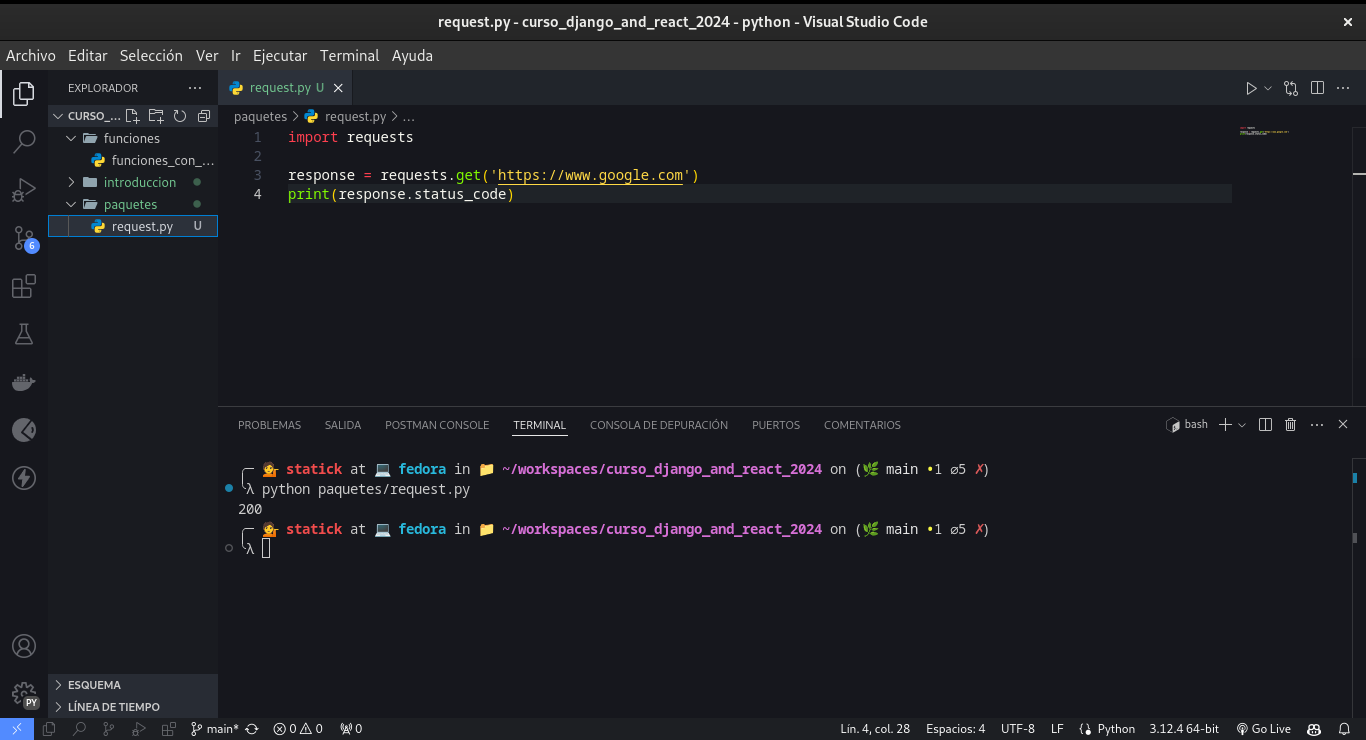
\includegraphics{unidades/unidad4/images/paste-1.png}

Para utilizar un paquete de Pypi, primero debes instalarlo usando
\textbf{pip}. Por ejemplo, si quieres instalar el paquete
\textbf{requests}, puedes hacerlo de la siguiente manera:

\begin{Shaded}
\begin{Highlighting}[]
\ExtensionTok{pip}\NormalTok{ install requests}
\end{Highlighting}
\end{Shaded}

Una vez que hayas instalado el paquete, puedes importarlo en tu código
de Python y utilizarlo. Por ejemplo:

\begin{Shaded}
\begin{Highlighting}[]
\ImportTok{import}\NormalTok{ requests}

\NormalTok{response }\OperatorTok{=}\NormalTok{ requests.get(}\StringTok{\textquotesingle{}https://www.google.com\textquotesingle{}}\NormalTok{)}
\BuiltInTok{print}\NormalTok{(response.status\_code)}
\end{Highlighting}
\end{Shaded}

Otro ejemplo es por ejemplo el paquete emoji, que te permite utilizar
emojis en tus programas de Python.

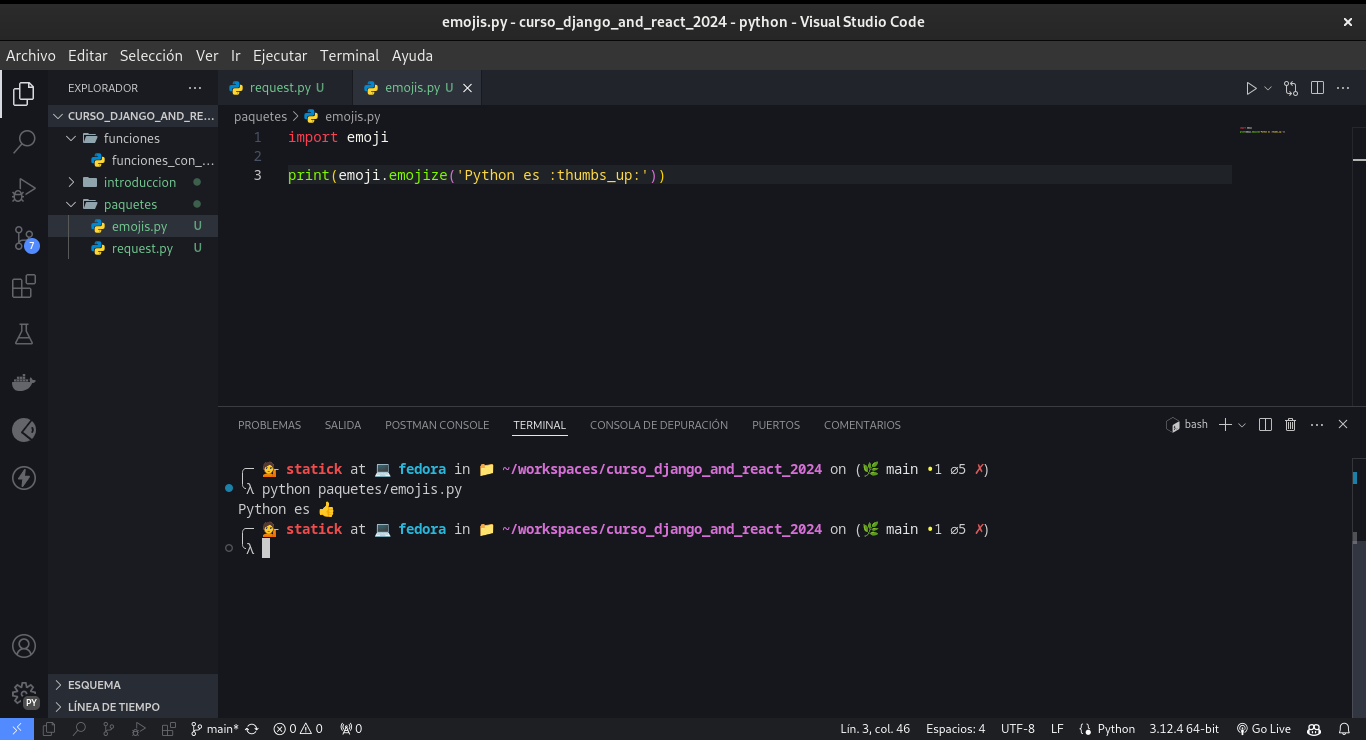
\includegraphics{unidades/unidad4/images/paste-2.png}

\begin{Shaded}
\begin{Highlighting}[]
\ExtensionTok{pip}\NormalTok{ install emoji}
\end{Highlighting}
\end{Shaded}

\begin{Shaded}
\begin{Highlighting}[]
\ImportTok{import}\NormalTok{ emoji}

\BuiltInTok{print}\NormalTok{(emoji.emojize(}\StringTok{\textquotesingle{}Python es :thumbs\_up:\textquotesingle{}}\NormalTok{))}
\end{Highlighting}
\end{Shaded}

¡Y eso es todo! Ahora puedes utilizar cualquier paquete de Python
disponible en Pypi en tus proyectos.

Algunos paquetes pueden ser muy importantes para tu proyecto, así que
asegúrate de revisar Pypi para encontrar los paquetes que necesitas.

\chapter{Conclusión}\label{conclusiuxf3n-1}

Pypi es un recurso valioso para los desarrolladores de Python. Te
permite compartir tus paquetes con otros desarrolladores y utilizar los
paquetes de otros desarrolladores en tus proyectos.

\chapter{Públicar un paquete en
Pypi}\label{puxfablicar-un-paquete-en-pypi}

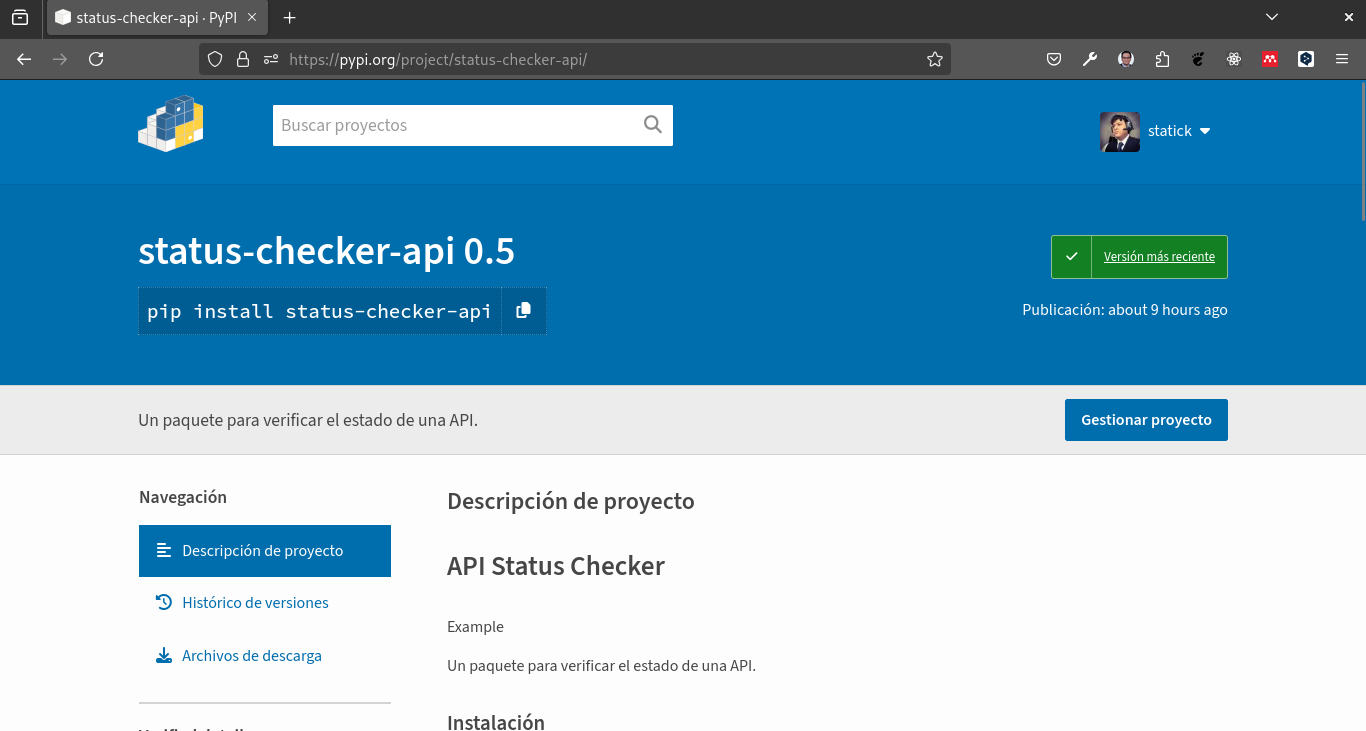
\includegraphics{unidades/unidad4/images/paste-10.png}

En este tutorial vamos a publicar un paquete llamado
\textbf{status-checker-api} en Pypi.

Si has creado un paquete de Python y quieres compartirlo con otros
desarrolladores, puedes publicarlo en Pypi.

Para ello vamos a crear un repositorio en \textbf{GitHub} y subir
nuestro paquete, esta práctica es importante para poder compartir
nuestro paquete con otros desarrolladores.

En el caso de este tutorial, el repositorio se encuentra en
\href{https://github.com/statick88/status_checker_api}{status\_checker\_api}

Lo más importante es tener el o los scripts que contienen el código que
queremos convertir a paquete.

Para ello vamos a empezar creando un directorio con el nombre de nuestro
paquete, por ejemplo \textbf{status\_checker\_api}.

A continuación se visualiza la estructura de nuestro paquete.

\begin{Shaded}
\begin{Highlighting}[]
\NormalTok{├── dist}
\NormalTok{│   ├── status\_checker\_api{-}0.5{-}py3{-}none{-}any.whl}
\NormalTok{│   └── status\_checker\_api{-}0.5.tar.gz}
\NormalTok{├── img}
\NormalTok{│   └── paste{-}5.png}
\NormalTok{├── LICENSE}
\NormalTok{├── README.md}
\NormalTok{├── setup.py}
\NormalTok{└── src}
\NormalTok{    ├── status\_checker\_api}
\NormalTok{    │   ├── \_\_init\_\_.py}
\NormalTok{    │   ├── \_\_main\_\_.py}
\NormalTok{    │   └── \_\_pycache\_\_}
\NormalTok{    │       ├── \_\_init\_\_.cpython{-}312.pyc}
\NormalTok{    │       └── \_\_main\_\_.cpython{-}312.pyc}
\NormalTok{    ├── status\_checker\_api.egg{-}info}
\NormalTok{    │   ├── dependency\_links.txt}
\NormalTok{    │   ├── entry\_points.txt}
\NormalTok{    │   ├── PKG{-}INFO}
\NormalTok{    │   ├── requires.txt}
\NormalTok{    │   ├── SOURCES.txt}
\NormalTok{    │   └── top\_level.txt}
\NormalTok{    └── tests}
\NormalTok{        ├── \_\_init\_\_.py}
\NormalTok{        ├── \_\_pycache\_\_}
\NormalTok{        │   ├── \_\_init\_\_.cpython{-}312.pyc}
\NormalTok{        │   └── test\_status\_checker\_api.cpython{-}312{-}pytest{-}8.3.2.pyc}
\NormalTok{        └── test\_status\_checker\_api.py}
\end{Highlighting}
\end{Shaded}

Dentro de este \textbf{status\_checker\_api} vamos a crear un directorio
llamado \textbf{src} y dentro de este directorio vamos a crear un
archivo llamado \textbf{\_\_init\_\_.py}, en este ejemplo tambien
crearemos el archivo \textbf{\_\_main\_\_.py}.

Para poder publicar nuestro paquete en Pypi, necesitamos crear un
archivo llamado \textbf{setup.py} en el directorio raíz de nuestro
paquete. Este archivo contiene la información necesaria para empaquetar
nuestro paquete y publicarlo en Pypi.

\begin{Shaded}
\begin{Highlighting}[]
\ImportTok{from}\NormalTok{ setuptools }\ImportTok{import}\NormalTok{ setup, find\_packages}

\ControlFlowTok{with} \BuiltInTok{open}\NormalTok{(}\StringTok{\textquotesingle{}README.md\textquotesingle{}}\NormalTok{, }\StringTok{\textquotesingle{}r\textquotesingle{}}\NormalTok{, encoding}\OperatorTok{=}\StringTok{"utf{-}8"}\NormalTok{) }\ImportTok{as}\NormalTok{ fh:}
\NormalTok{    long\_description }\OperatorTok{=}\NormalTok{ fh.read()}

\NormalTok{setup(}
\NormalTok{    name}\OperatorTok{=}\StringTok{\textquotesingle{}status\_checker\_api\textquotesingle{}}\NormalTok{,}
\NormalTok{    version}\OperatorTok{=}\StringTok{\textquotesingle{}0.5\textquotesingle{}}\NormalTok{,}
\NormalTok{    packages}\OperatorTok{=}\NormalTok{find\_packages(where}\OperatorTok{=}\StringTok{\textquotesingle{}src\textquotesingle{}}\NormalTok{),}
\NormalTok{    package\_dir}\OperatorTok{=}\NormalTok{\{}\StringTok{\textquotesingle{}\textquotesingle{}}\NormalTok{: }\StringTok{\textquotesingle{}src\textquotesingle{}}\NormalTok{\},}
\NormalTok{    install\_requires}\OperatorTok{=}\NormalTok{[}
        \StringTok{\textquotesingle{}requests\textquotesingle{}}\NormalTok{,}
\NormalTok{    ],}
\NormalTok{    entry\_points}\OperatorTok{=}\NormalTok{\{}
        \StringTok{\textquotesingle{}console\_scripts\textquotesingle{}}\NormalTok{: [}
            \StringTok{\textquotesingle{}status{-}checker{-}api=status\_checker\_api.\_\_main\_\_:main\textquotesingle{}}\NormalTok{,}
\NormalTok{        ],}
\NormalTok{    \},}
\NormalTok{    author}\OperatorTok{=}\StringTok{\textquotesingle{}Diego Saavedra\textquotesingle{}}\NormalTok{,}
\NormalTok{    author\_email}\OperatorTok{=}\StringTok{\textquotesingle{}dsaavedra88@gmail.com\textquotesingle{}}\NormalTok{,}
\NormalTok{    description}\OperatorTok{=}\StringTok{\textquotesingle{}Un paquete para verificar el estado de una API.\textquotesingle{}}\NormalTok{,}
\NormalTok{    long\_description}\OperatorTok{=}\NormalTok{long\_description,}
\NormalTok{    long\_description\_content\_type}\OperatorTok{=}\StringTok{\textquotesingle{}text/markdown\textquotesingle{}}\NormalTok{,}
\NormalTok{    url}\OperatorTok{=}\StringTok{\textquotesingle{}https://github.com/statick88/status\_checker\_api\textquotesingle{}}\NormalTok{,}
\NormalTok{    classifiers}\OperatorTok{=}\NormalTok{[}
        \StringTok{\textquotesingle{}Programming Language :: Python :: 3\textquotesingle{}}\NormalTok{,}
        \StringTok{\textquotesingle{}License :: OSI Approved :: MIT License\textquotesingle{}}\NormalTok{,}
        \StringTok{\textquotesingle{}Operating System :: OS Independent\textquotesingle{}}\NormalTok{,}
\NormalTok{    ],}
\NormalTok{    options}\OperatorTok{=}\NormalTok{\{}
        \StringTok{\textquotesingle{}egg\_info\textquotesingle{}}\NormalTok{: \{}
            \StringTok{\textquotesingle{}egg\_base\textquotesingle{}}\NormalTok{: }\StringTok{\textquotesingle{}src\textquotesingle{}}
\NormalTok{        \}}
\NormalTok{    \},}
\NormalTok{    python\_requires}\OperatorTok{=}\StringTok{\textquotesingle{}\textgreater{}=3.12\textquotesingle{}}\NormalTok{,}
\NormalTok{)}
\end{Highlighting}
\end{Shaded}

\chapter{Creación del archivo
README.md}\label{creaciuxf3n-del-archivo-readme.md}

\begin{Shaded}
\begin{Highlighting}[]
\FunctionTok{\# status\_checker\_api}

\NormalTok{Un paquete para verificar el estado de una API.}

\FunctionTok{\#\# Instalación}

\NormalTok{pip install status\_checker\_api}

\FunctionTok{\#\# Uso}

\NormalTok{api{-}status{-}checker}

\NormalTok{Ingrese la URL de la API: https://www.google.com}

\NormalTok{El status de la API es: 200}

\FunctionTok{\#\# Licencia}

\NormalTok{MIT License}

\FunctionTok{\#\# Autor}

\NormalTok{Diego Saavedra}
\end{Highlighting}
\end{Shaded}

El código del paquete se encuentra en el directorio \textbf{src}. Para
poder ejecutar el paquete, necesitamos un archivo llamado
\textbf{\_\_init\_\_.py} en el directorio \textbf{status\_checker\_api}.

\begin{Shaded}
\begin{Highlighting}[]
\ImportTok{import}\NormalTok{ requests}
\ImportTok{from}\NormalTok{ urllib.parse }\ImportTok{import}\NormalTok{ urlparse}

\KeywordTok{def}\NormalTok{ check\_status(url):}
    \CommentTok{\# Asegúrate de que la URL tenga un esquema (http o https)}
\NormalTok{    parsed\_url }\OperatorTok{=}\NormalTok{ urlparse(url)}
    \ControlFlowTok{if} \KeywordTok{not}\NormalTok{ parsed\_url.scheme:}
\NormalTok{        url }\OperatorTok{=} \StringTok{\textquotesingle{}https://\textquotesingle{}} \OperatorTok{+}\NormalTok{ url}
    
    \ControlFlowTok{try}\NormalTok{:}
\NormalTok{        response }\OperatorTok{=}\NormalTok{ requests.get(url)}
        \ControlFlowTok{return} \SpecialStringTok{f"La URL está activa con código de estado: }\SpecialCharTok{\{}\NormalTok{response}\SpecialCharTok{.}\NormalTok{status\_code}\SpecialCharTok{\}}\SpecialStringTok{"}  \CommentTok{\# Devuelve el mensaje con el código de estado}
    \ControlFlowTok{except}\NormalTok{ requests.exceptions.RequestException }\ImportTok{as}\NormalTok{ e:}
        \ControlFlowTok{return} \SpecialStringTok{f"Error: }\SpecialCharTok{\{}\NormalTok{e}\SpecialCharTok{\}}\SpecialStringTok{"}  \CommentTok{\# Devuelve el mensaje de error con una x}
\end{Highlighting}
\end{Shaded}

Analizando el código anterior, podemos ver que el paquete
\textbf{status\_checker\_api} contiene una función llamada
\textbf{check\_status} que verifica el estado de una API. La función
toma una URL como argumento y devuelve un mensaje con el estado de la
API.

\chapter{Creación del archivo
\_\_main\_\_.py}\label{creaciuxf3n-del-archivo-__main__.py}

\begin{Shaded}
\begin{Highlighting}[]
\ImportTok{from}\NormalTok{ status\_checker\_api }\ImportTok{import}\NormalTok{ check\_status}

\KeywordTok{def}\NormalTok{ main():}
\NormalTok{    url }\OperatorTok{=} \BuiltInTok{input}\NormalTok{(}\StringTok{\textquotesingle{}Ingrese la URL de la API: \textquotesingle{}}\NormalTok{)}
\NormalTok{    status }\OperatorTok{=}\NormalTok{ check\_status(url)}
    \BuiltInTok{print}\NormalTok{(}\SpecialStringTok{f\textquotesingle{}El status de la API es: }\SpecialCharTok{\{}\NormalTok{status}\SpecialCharTok{\}}\SpecialStringTok{\textquotesingle{}}\NormalTok{)}

\ControlFlowTok{if} \VariableTok{\_\_name\_\_} \OperatorTok{==} \StringTok{"\_\_main\_\_"}\NormalTok{:}
\NormalTok{    main()}
\end{Highlighting}
\end{Shaded}

El archivo \textbf{\_\_main\_\_.py} contiene el código principal del
paquete. Este archivo importa la función \textbf{check\_status} del
paquete \textbf{status\_checker\_api} y la utiliza para verificar el
estado de una API.

\chapter{Creación del archivo
LICENSE}\label{creaciuxf3n-del-archivo-license}

\begin{Shaded}
\begin{Highlighting}[]
\NormalTok{MIT License}

\NormalTok{Copyright (c) 2024 Diego Saavedra}

\NormalTok{Permission is hereby granted, free of charge, to any person obtaining a copy}
\NormalTok{of this software and associated documentation files (the "Software"), to deal}
\NormalTok{in the Software without restriction, including without limitation the rights}
\NormalTok{to use, copy, modify, merge, publish, distribute, sublicense, and/or sell}
\NormalTok{copies of the Software, and to permit persons to whom the Software is}
\NormalTok{furnished to do so, subject to the following conditions:}

\NormalTok{The above copyright notice and this permission notice shall be included in all}

\NormalTok{copies or substantial portions of the Software.}
\end{Highlighting}
\end{Shaded}

El archivo \textbf{LICENSE} contiene la licencia del paquete. En este
caso, utilizamos la licencia MIT.

\chapter{Creación del archivo
.gitignore}\label{creaciuxf3n-del-archivo-.gitignore}

\begin{Shaded}
\begin{Highlighting}[]
\NormalTok{\# Byte{-}compiled / optimized / DLL files}
\NormalTok{\_\_pycache\_\_/}
\NormalTok{*.py[cod]}
\NormalTok{*$py.class}

\NormalTok{\# C extensions}
\NormalTok{*.so}

\NormalTok{\# Distribution / packaging}
\NormalTok{dist/}
\NormalTok{build/}
\NormalTok{*.egg{-}info/}
\NormalTok{*.egg}

\NormalTok{\# Virtual environments}
\NormalTok{venv/}
\NormalTok{env/}
\NormalTok{ENV/}

\NormalTok{\# IDEs / Editors}
\NormalTok{.idea/}
\NormalTok{.vscode/}
\NormalTok{*.sublime{-}project}
\NormalTok{*.sublime{-}workspace}

\NormalTok{\# Miscellaneous}
\NormalTok{*.swp}
\NormalTok{.DS\_Store}
\end{Highlighting}
\end{Shaded}

El archivo \textbf{.gitignore} contiene los archivos y directorios que
no queremos incluir en nuestro repositorio de Git. En este caso,
ignoramos los archivos y directorios generados por Python y los entornos
virtuales.

\chapter{Creación de la cuenta en
Pypi}\label{creaciuxf3n-de-la-cuenta-en-pypi}

Para poder publicar nuestro paquete en Pypi, necesitamos crear una
cuenta en \href{https://pypi.org/account/register/}{Pypi}.

\begin{tcolorbox}[enhanced jigsaw, bottomrule=.15mm, title=\textcolor{quarto-callout-tip-color}{\faLightbulb}\hspace{0.5em}{Tip}, coltitle=black, leftrule=.75mm, left=2mm, colbacktitle=quarto-callout-tip-color!10!white, breakable, colframe=quarto-callout-tip-color-frame, colback=white, opacitybacktitle=0.6, opacityback=0, bottomtitle=1mm, toptitle=1mm, toprule=.15mm, arc=.35mm, titlerule=0mm, rightrule=.15mm]

Una vez creada la cuenta en Pypi, necesitamos verificarla a través de un
correo electrónico que nos enviarán. Adicional a ello es necesario
configurar un factor de doble autenticación. Esto es indispensable para
poder crear un token de acceso. El mismo que nos permitirá subir nuestro
paquete a Pypi.

\end{tcolorbox}

Una vez que hayamos creado la cuenta, necesitamos crear un archivo
llamado \textbf{.pypirc} en nuestro directorio de usuario con la
siguiente información:

\begin{Shaded}
\begin{Highlighting}[]
\NormalTok{[pypi]}
\NormalTok{  username = statick}
\NormalTok{  password = pypi{-}token}
\end{Highlighting}
\end{Shaded}

En el archivo \textbf{.pypirc}, reemplazamos \textbf{username} con
nuestro nombre de usuario de Pypi y \textbf{password} con nuestro token
de acceso de Pypi.

\begin{tcolorbox}[enhanced jigsaw, bottomrule=.15mm, title=\textcolor{quarto-callout-tip-color}{\faLightbulb}\hspace{0.5em}{Tip}, coltitle=black, leftrule=.75mm, left=2mm, colbacktitle=quarto-callout-tip-color!10!white, breakable, colframe=quarto-callout-tip-color-frame, colback=white, opacitybacktitle=0.6, opacityback=0, bottomtitle=1mm, toptitle=1mm, toprule=.15mm, arc=.35mm, titlerule=0mm, rightrule=.15mm]

En sistemas operativos basados en Unix, el archivo \textbf{.pypirc} se
encuentra en el directorio de usuario \textbf{.pypirc}.

En sistemas operativos basados en Windows, el archivo \textbf{.pypirc}
se encuentra en el directorio de usuario
\textbf{C:}/\Users/\username.pypirc.

\end{tcolorbox}

\chapter{Publicar el paquete en Pypi}\label{publicar-el-paquete-en-pypi}

Para publicar nuestro paquete en Pypi, necesitamos instalar el paquete
\textbf{twine}.

Twine es una herramienta que nos permite subir paquetes de Python a
Pypi.

\begin{Shaded}
\begin{Highlighting}[]
\ExtensionTok{pip}\NormalTok{ install twine}
\end{Highlighting}
\end{Shaded}

Es recomandable que tengamos la última versión de \textbf{twine}.

\begin{Shaded}
\begin{Highlighting}[]
\ExtensionTok{pip}\NormalTok{ install }\AttributeTok{{-}{-}upgrade}\NormalTok{ twine}
\end{Highlighting}
\end{Shaded}

Una vez que hayamos instalado y actualizado \textbf{twine}, podemos
publicar nuestro paquete en Pypi de la siguiente manera:

\begin{Shaded}
\begin{Highlighting}[]
\ExtensionTok{python} \AttributeTok{{-}m}\NormalTok{ pip install }\AttributeTok{{-}{-}upgrade}\NormalTok{ build}
\end{Highlighting}
\end{Shaded}

El comando anterior instala el paquete \textbf{build} que necesitamos
para construir nuestro paquete.

\begin{Shaded}
\begin{Highlighting}[]
\ExtensionTok{python} \AttributeTok{{-}m}\NormalTok{ build}
\end{Highlighting}
\end{Shaded}

El comando anterior crea un archivo \textbf{dist} en el directorio raíz
de nuestro paquete. Este archivo contiene el paquete que vamos a
publicar en Pypi. Es decir los archivos \textbf{.tar.gz} y
\textbf{.whl}.

Estos archivos son los que vamos a subir a Pypi.

\begin{Shaded}
\begin{Highlighting}[]
\ExtensionTok{python} \AttributeTok{{-}m}\NormalTok{ twine upload }\AttributeTok{{-}{-}repository}\NormalTok{ pypi dist/}\PreprocessorTok{*} \AttributeTok{{-}{-}verbose}
\end{Highlighting}
\end{Shaded}

El comando anterior sube nuestro paquete a Pypi. El archivo
\textbf{.pypirc} contiene la información de autenticación que
necesitamos para subir nuestro paquete.

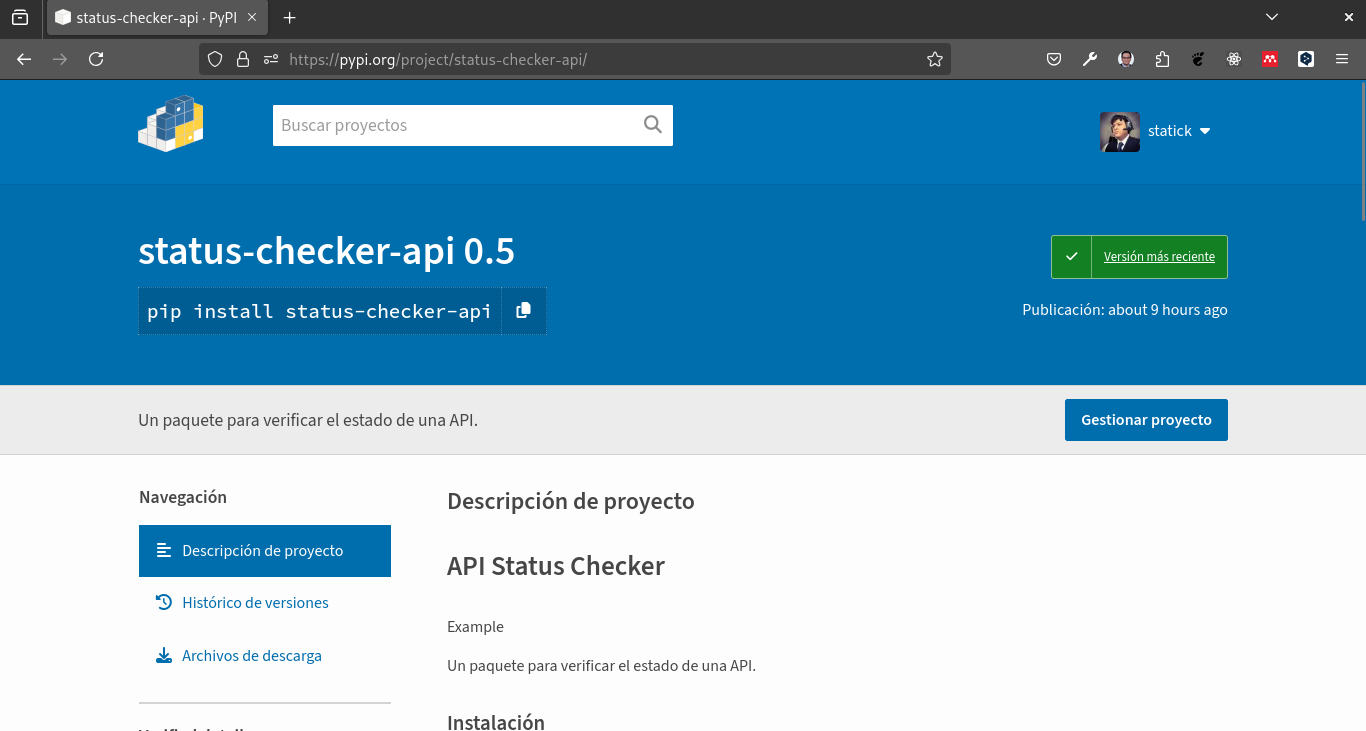
\includegraphics{unidades/unidad4/images/paste-10.png}

¡Y eso es todo! Ahora puedes compartir tu paquete de Python con otros
desarrolladores en Pypi. En el caso de este paquete la url es
\href{https://pypi.org/project/status-checker-api/}{status\_checker\_api}.

\chapter{Instalar el paquete}\label{instalar-el-paquete}

Para instalar el paquete que acabamos de publicar en Pypi, necesitamos
usar \textbf{pip}.

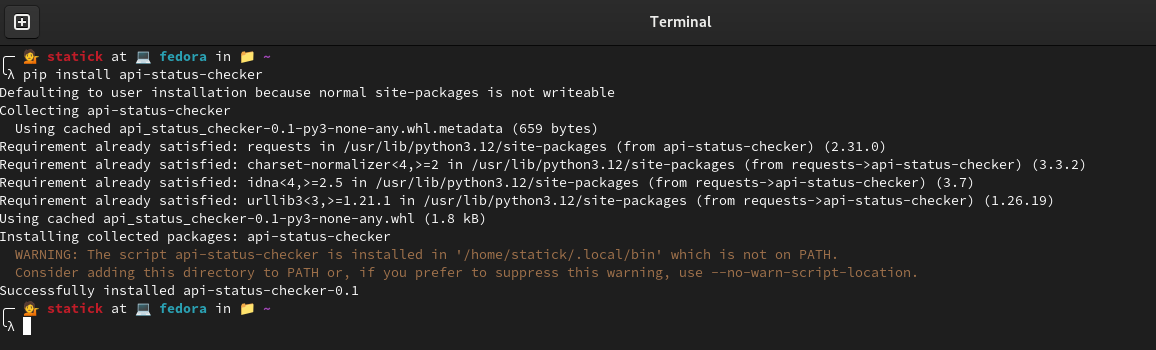
\includegraphics{unidades/unidad4/images/paste-4.png}

\begin{Shaded}
\begin{Highlighting}[]
\ExtensionTok{pip}\NormalTok{ install status\_checker\_api}
\end{Highlighting}
\end{Shaded}

Una vez que hayamos instalado el paquete, podemos utilizarlo en nuestro
código de Python.

\chapter{Uso del paquete}\label{uso-del-paquete}

\begin{Shaded}
\begin{Highlighting}[]
\ExtensionTok{api{-}status{-}checker}
\end{Highlighting}
\end{Shaded}

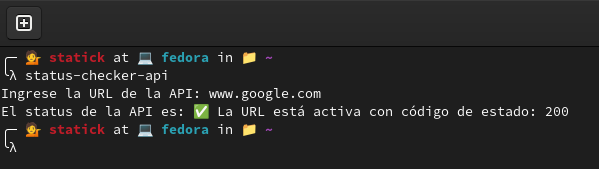
\includegraphics{unidades/unidad4/images/paste-11.png}

Es necesario ingresar la URL de la API que queremos verificar.

\textbf{Ingrese la URL de la API:} https://www.google.com

\textbf{El status de la API es:} 200

¡Y eso es todo! Ahora puedes actualizar tu paquete de Python en Pypi.

\begin{tcolorbox}[enhanced jigsaw, bottomrule=.15mm, title=\textcolor{quarto-callout-tip-color}{\faLightbulb}\hspace{0.5em}{Tip}, coltitle=black, leftrule=.75mm, left=2mm, colbacktitle=quarto-callout-tip-color!10!white, breakable, colframe=quarto-callout-tip-color-frame, colback=white, opacitybacktitle=0.6, opacityback=0, bottomtitle=1mm, toptitle=1mm, toprule=.15mm, arc=.35mm, titlerule=0mm, rightrule=.15mm]

No olvides cambiar la versión de tu paquete en el archivo
\textbf{setup.py} antes de subirlo a Pypi si realizas alguna
actualización.

\end{tcolorbox}

Si decidimos actualizar el paquete en Pypi, necesitamos seguir los
mismos pasos que hemos visto en este tutorial.

Sin embargo solo necesitaremos 2 comandos:

\begin{Shaded}
\begin{Highlighting}[]
\ExtensionTok{python} \AttributeTok{{-}m}\NormalTok{ build}
\end{Highlighting}
\end{Shaded}

\begin{Shaded}
\begin{Highlighting}[]
\ExtensionTok{python} \AttributeTok{{-}m}\NormalTok{ twine upload }\AttributeTok{{-}{-}repository}\NormalTok{ pypi dist/}\PreprocessorTok{*} \AttributeTok{{-}{-}verbose}
\end{Highlighting}
\end{Shaded}

\begin{tcolorbox}[enhanced jigsaw, bottomrule=.15mm, title=\textcolor{quarto-callout-tip-color}{\faLightbulb}\hspace{0.5em}{Tip}, coltitle=black, leftrule=.75mm, left=2mm, colbacktitle=quarto-callout-tip-color!10!white, breakable, colframe=quarto-callout-tip-color-frame, colback=white, opacitybacktitle=0.6, opacityback=0, bottomtitle=1mm, toptitle=1mm, toprule=.15mm, arc=.35mm, titlerule=0mm, rightrule=.15mm]

En el directorio dist se generan los archivos \textbf{.tar.gz} y
\textbf{.whl} que son los que vamos a subir a Pypi. Es necesario
eliminar los archivos anteriores antes de subir los nuevos en este
directorio, mi recomendación es eliminar el directorio \textbf{dist} y
volver a ejecutar el comando \textbf{python -m build}.

\end{tcolorbox}

\chapter{Conclusión}\label{conclusiuxf3n-2}

En este tutorial aprendimos cómo publicar un paquete de Python en Pypi.
Pudimos ver cómo crear un paquete de Python, subirlo a Pypi y
compartirlo con otros desarrolladores.

\chapter{Sistema de Gestión de
Inventarios}\label{sistema-de-gestiuxf3n-de-inventarios}

\section{Asignación}\label{asignaciuxf3n-5}

\url{https://classroom.github.com/a/OVCpAmrV}

Aprenderás a desarrollar un proyecto de utilizando el lenguaje de
programación Python.

Un sistema de gestión de inventarios es una herramienta que permite
realizar un seguimiento y control de los productos o artículos
almacenados en un negocio o empresa.

Aprenderás a utilizar diferentes conceptos y técnicas de programación
para implementar las funcionalidades clave de este sistema.

Algunas de las funcionalidades que implementaremos incluyen:

Aprenderás a crear una estructura de datos para almacenar la información
de los productos, como su nombre, descripción, precio, cantidad
disponible, etc. También aprenderás a agregar nuevos productos al
sistema.

Te enseñaré cómo implementar funciones de búsqueda y filtrado para
encontrar productos específicos en base a diferentes criterios, como el
nombre, la categoría o el precio.

Aprenderás a manejar las actualizaciones de inventario, como la compra o
venta de productos. Implementaremos funciones que permitan aumentar o
disminuir la cantidad disponible de un producto y mantener un registro
de estas transacciones.

Te mostraré cómo generar informes sobre el estado del inventario, como
la lista de productos disponibles, los productos más vendidos, los
productos con bajo stock, etc. Utilizaremos técnicas de manipulación de
datos y generación de informes para presentar esta información de manera
clara y concisa.

\part{Unidad 5: Django}

\chapter{Introducción a Django}\label{introducciuxf3n-a-django}

\begin{figure}[H]

{\centering 
\includegraphics[width=2.08333in,height=\textheight]{images/django-logo.png}

}

\caption{Django Framework}

\end{figure}%

Django es un framework web de alto nivel que fomenta el desarrollo
rápido y limpio. Es un framework web de alto nivel que fomenta el
desarrollo rápido y limpio. Diseñado por desarrolladores experimentados,
Django se encarga de gran parte de la molestia del desarrollo web, por
lo que puedes concentrarte en escribir tu aplicación sin necesidad de
reinventar la rueda. Es gratuito y de código abierto, tiene una
comunidad activa y amigable, y es utilizado por algunas de las mayores
empresas del mundo.

\section{Conceptos Importantes}\label{conceptos-importantes}

\begin{tcolorbox}[enhanced jigsaw, bottomrule=.15mm, title=\textcolor{quarto-callout-tip-color}{\faLightbulb}\hspace{0.5em}{Tip}, coltitle=black, leftrule=.75mm, left=2mm, colbacktitle=quarto-callout-tip-color!10!white, breakable, colframe=quarto-callout-tip-color-frame, colback=white, opacitybacktitle=0.6, opacityback=0, bottomtitle=1mm, toptitle=1mm, toprule=.15mm, arc=.35mm, titlerule=0mm, rightrule=.15mm]

Antes de iniciar con Django es necesario conocer el concepto de
\textbf{Entornos Virtuales}.

\end{tcolorbox}

\subsection{Entornos Virtuales}\label{entornos-virtuales}

\begin{figure}[H]

{\centering 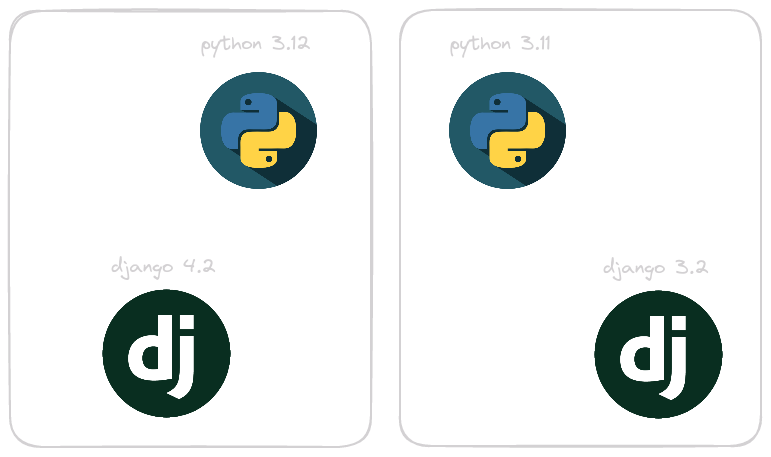
\includegraphics[width=4.16667in,height=\textheight]{images/python-venv.png}

}

\caption{Virtual Enviroment}

\end{figure}%

Un entorno virtual es un \textbf{entorno de desarrollo aislado }que
permite \textbf{instalar paquetes de Python sin afectar al sistema
global}. Los entornos virtuales son útiles para gestionar las
dependencias de un proyecto y para evitar conflictos entre diferentes
versiones de los paquetes.

\subsubsection{Crear un entorno virtual}\label{crear-un-entorno-virtual}

Para crear un entorno virtual, se puede utilizar la herramienta
\textbf{venv} de Python.

\begin{Shaded}
\begin{Highlighting}[]
\ExtensionTok{python} \AttributeTok{{-}m}\NormalTok{ venv env}
\end{Highlighting}
\end{Shaded}

Este comando creará un directorio llamado \textbf{env} en el directorio
actual con el entorno virtual.

\begin{tcolorbox}[enhanced jigsaw, bottomrule=.15mm, title=\textcolor{quarto-callout-tip-color}{\faLightbulb}\hspace{0.5em}{Tip}, coltitle=black, leftrule=.75mm, left=2mm, colbacktitle=quarto-callout-tip-color!10!white, breakable, colframe=quarto-callout-tip-color-frame, colback=white, opacitybacktitle=0.6, opacityback=0, bottomtitle=1mm, toptitle=1mm, toprule=.15mm, arc=.35mm, titlerule=0mm, rightrule=.15mm]

Tambien se puede utilizar
\href{https://pypi.org/project/virtualenv/}{virtualenv} para crear
entornos virtuales.

\end{tcolorbox}

\subsection{Modelo Template View (MTV)}\label{modelo-template-view-mtv}

\begin{figure}[H]

{\centering 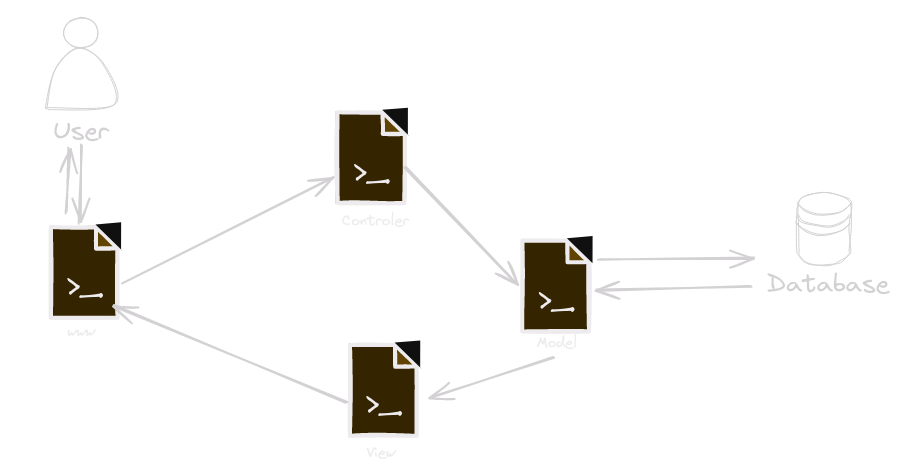
\includegraphics[width=4.16667in,height=\textheight]{images/model-view-controller.png}

}

\caption{Model View Controller}

\end{figure}%

\begin{figure}[H]

{\centering 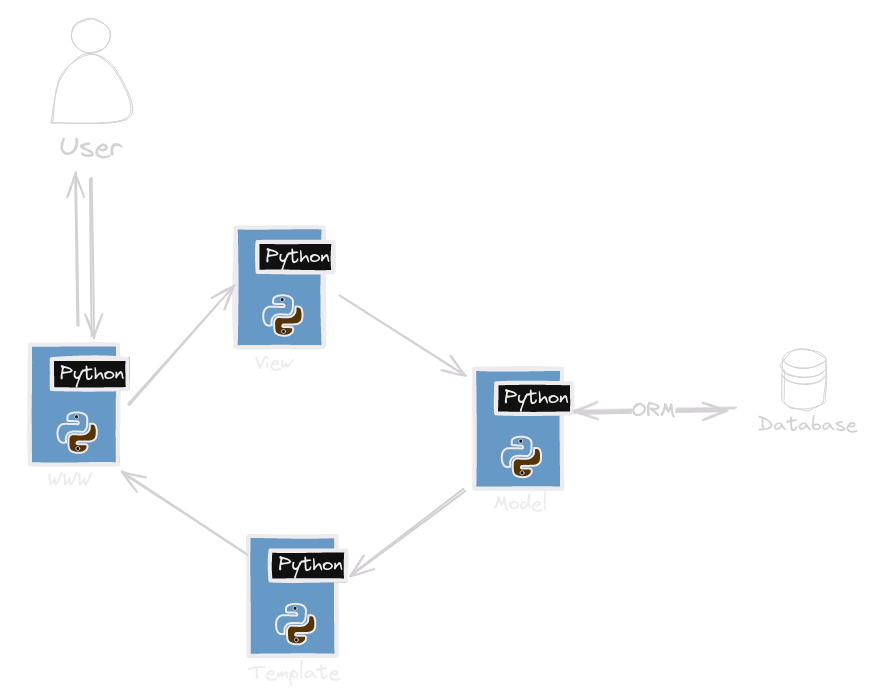
\includegraphics[width=4.16667in,height=\textheight]{images/model-template-view.png}

}

\caption{Model View Template}

\end{figure}%

Django sigue el patrón de diseño Modelo Vista Template (MVT). Este
patrón de diseño separa la lógica de la aplicación en tres componentes
principales: Modelo, Vista y Template.

\begin{tcolorbox}[enhanced jigsaw, bottomrule=.15mm, title=\textcolor{quarto-callout-tip-color}{\faLightbulb}\hspace{0.5em}{Tip}, coltitle=black, leftrule=.75mm, left=2mm, colbacktitle=quarto-callout-tip-color!10!white, breakable, colframe=quarto-callout-tip-color-frame, colback=white, opacitybacktitle=0.6, opacityback=0, bottomtitle=1mm, toptitle=1mm, toprule=.15mm, arc=.35mm, titlerule=0mm, rightrule=.15mm]

El archivo URLs.py es el encargado de mapear las URLs de la aplicación a
las vistas correspondientes.

\end{tcolorbox}

\begin{itemize}
\item
  \textbf{Modelo}: Es la representación de los datos de la aplicación y
  las reglas para manipular esos datos. Django utiliza un ORM
  (Object-Relational Mapping) para interactuar con la base de datos.
\item
  \textbf{Vista}: Es la capa de presentación de la aplicación. Se
  encarga de mostrar los datos al usuario y de interpretar las acciones
  del usuario.
\item
  \textbf{Template}: Es la capa de presentación de la aplicación. Define
  cómo se muestra la información al usuario. Django utiliza el motor de
  plantillas Jinja2 para renderizar los templates.
\end{itemize}

\subsection{Formularios}\label{formularios}

\begin{figure}[H]

{\centering 
\includegraphics{images/python-form.png}

}

\caption{Django Forms}

\end{figure}%

Los formularios son una parte importante de cualquier aplicación web.
Django proporciona una forma sencilla de crear y procesar formularios en
las vistas.

\subsection{Administrador de Django}\label{administrador-de-django}

\begin{figure}[H]

{\centering 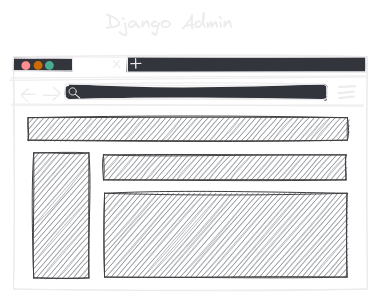
\includegraphics{images/django-admin.png}

}

\caption{Django Admin}

\end{figure}%

El administrador de Django es una interfaz de administración que permite
gestionar los datos de la aplicación de forma sencilla. Django genera
automáticamente una interfaz de administración basada en los modelos de
la aplicación.

\subsection{Middleware}\label{middleware}

El middleware es una capa de procesamiento que se ejecuta antes y
después de cada petición HTTP. Django proporciona un conjunto de
middlewares que se pueden utilizar para añadir funcionalidades a la
aplicación.

\subsection{Autenticación y
Autorización}\label{autenticaciuxf3n-y-autorizaciuxf3n}

Django proporciona un sistema de autenticación y autorización que
permite gestionar los usuarios y los permisos de la aplicación de forma
sencilla.

\subsection{Internacionalización}\label{internacionalizaciuxf3n}

Django proporciona soporte para la internacionalización de la
aplicación. Permite traducir la aplicación a diferentes idiomas y
gestionar las traducciones de forma sencilla.

\subsection{Seguridad}\label{seguridad}

Django proporciona un conjunto de medidas de seguridad para proteger la
aplicación contra ataques comunes, como la inyección de SQL, la
falsificación de solicitudes entre sitios (CSRF) y la inyección de
código.

\subsection{Testing}\label{testing}

Django proporciona un conjunto de herramientas para realizar pruebas
unitarias y de integración en la aplicación. Permite probar la lógica de
la aplicación y asegurarse de que funciona correctamente.

\subsection{Despliegue}\label{despliegue}

Django proporciona un conjunto de herramientas para desplegar la
aplicación en un servidor de producción. Permite configurar el entorno
de producción y gestionar las actualizaciones de la aplicación de forma
sencilla.

\chapter{Configuración inicial de un
proyecto.}\label{configuraciuxf3n-inicial-de-un-proyecto.}

\section{1. Crear un entorno virtual}\label{crear-un-entorno-virtual-1}

\begin{figure}[H]

{\centering 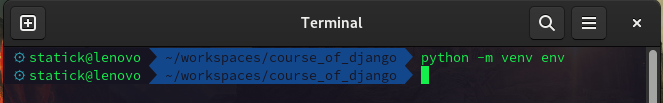
\includegraphics{images/creacion_entorno_virtual.png}

}

\caption{Creación de entorno Virtual}

\end{figure}%

\begin{Shaded}
\begin{Highlighting}[]
\ExtensionTok{python3} \AttributeTok{{-}m}\NormalTok{ venv env}
\end{Highlighting}
\end{Shaded}

El comando anterior creará un directorio llamado \textbf{env} en el
directorio actual, que contendrá un entorno virtual de Python.

\section{2. Activar el entorno
virtual}\label{activar-el-entorno-virtual}

\begin{figure}[H]

{\centering 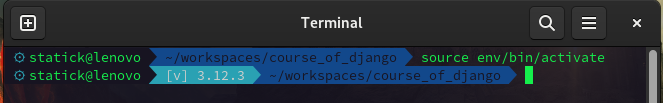
\includegraphics{images/activacion_entorno_virtual.png}

}

\caption{Activación de entorno Virtual}

\end{figure}%

\begin{Shaded}
\begin{Highlighting}[]
\BuiltInTok{source}\NormalTok{ env/bin/activate}
\end{Highlighting}
\end{Shaded}

El comando anterior activará el entorno virtual en sistemas Unix. En
Windows, el comando es:

\begin{Shaded}
\begin{Highlighting}[]
\FunctionTok{env}\DataTypeTok{\textbackslash{}S}\NormalTok{cripts}\DataTypeTok{\textbackslash{}a}\NormalTok{ctivate}
\end{Highlighting}
\end{Shaded}

Este comando tambien se puede dividir en 2 partes:

\begin{Shaded}
\begin{Highlighting}[]
\BuiltInTok{cd}\NormalTok{ env/Scripts/}
\ExtensionTok{activate}
\end{Highlighting}
\end{Shaded}

Para desactivar el entorno virtual, simplemente ejecute:

\begin{Shaded}
\begin{Highlighting}[]
\ExtensionTok{deactivate}
\end{Highlighting}
\end{Shaded}

\section{3. Instalar Django}\label{instalar-django}

\begin{figure}[H]

{\centering 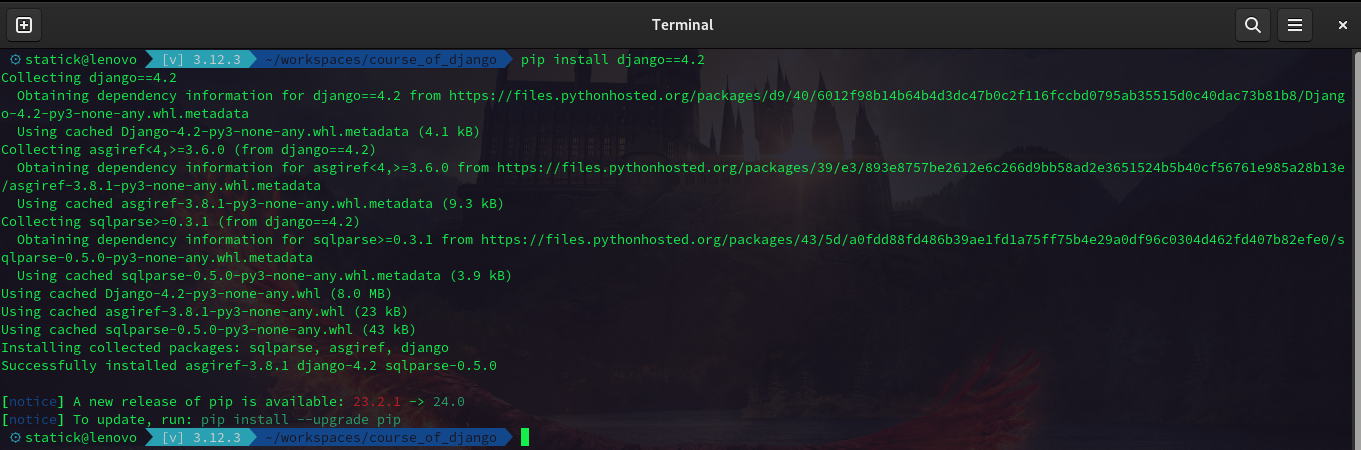
\includegraphics{images/instalacion_django.png}

}

\caption{Instalación de Django}

\end{figure}%

\begin{Shaded}
\begin{Highlighting}[]
\ExtensionTok{pip}\NormalTok{ install django==4.2}
\end{Highlighting}
\end{Shaded}

El comando anterior instalará la última versión de Django en el entorno
virtual.

\section{4. Crear un proyecto de
Django}\label{crear-un-proyecto-de-django}

\begin{figure}[H]

{\centering 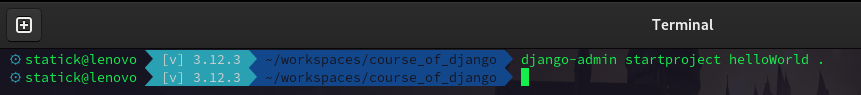
\includegraphics{images/creacion_project_django.png}

}

\caption{Creación de un Proyecto en Django}

\end{figure}%

\begin{Shaded}
\begin{Highlighting}[]
\ExtensionTok{django{-}admin}\NormalTok{ startproject helloWorld .}
\end{Highlighting}
\end{Shaded}

El comando anterior creará un nuevo directorio llamado
\textbf{helloWorld} en el directorio actual, que contendrá un proyecto
de Django.

\section{5. Crear una aplicación de
Django}\label{crear-una-aplicaciuxf3n-de-django}

\begin{figure}[H]

{\centering \includegraphics{images/creacion_app_django.png}

}

\caption{Creación de una App en Django}

\end{figure}%

\begin{Shaded}
\begin{Highlighting}[]
\ExtensionTok{python}\NormalTok{ manage.py startapp hello}
\end{Highlighting}
\end{Shaded}

El comando anterior creará un nuevo directorio llamado \textbf{hello} en
el directorio actual, que contendrá una aplicación de Django.

\begin{tcolorbox}[enhanced jigsaw, bottomrule=.15mm, title=\textcolor{quarto-callout-tip-color}{\faLightbulb}\hspace{0.5em}{Tip}, coltitle=black, leftrule=.75mm, left=2mm, colbacktitle=quarto-callout-tip-color!10!white, breakable, colframe=quarto-callout-tip-color-frame, colback=white, opacitybacktitle=0.6, opacityback=0, bottomtitle=1mm, toptitle=1mm, toprule=.15mm, arc=.35mm, titlerule=0mm, rightrule=.15mm]

Recerda que puedes abrir el editor de código Visual Studio Code con el
comando \textbf{code .}

\end{tcolorbox}

\section{6. Crear una vista}\label{crear-una-vista}

\begin{figure}[H]

{\centering \includegraphics{images/views_hello.png}

}

\caption{Vistas en Django}

\end{figure}%

\begin{Shaded}
\begin{Highlighting}[]
\CommentTok{\# hello/views.py}

\ImportTok{from}\NormalTok{ django.http }\ImportTok{import}\NormalTok{ HttpResponse}

\KeywordTok{def}\NormalTok{ index(request):}
    \ControlFlowTok{return}\NormalTok{ HttpResponse(}\StringTok{"Hello, World!"}\NormalTok{)}
\end{Highlighting}
\end{Shaded}

\section{7. Configurar las URL}\label{configurar-las-url}

\begin{figure}[H]

{\centering \includegraphics{images/urls_app_django.png}

}

\caption{URLs de la App en Django}

\end{figure}%

\begin{Shaded}
\begin{Highlighting}[]
\CommentTok{\# helloWorld/urls.py}

\ImportTok{from}\NormalTok{ django.contrib }\ImportTok{import}\NormalTok{ admin}
\ImportTok{from}\NormalTok{ django.urls }\ImportTok{import}\NormalTok{ include, path}

\NormalTok{urlpatterns }\OperatorTok{=}\NormalTok{ [}
\NormalTok{    path(}\StringTok{""}\NormalTok{, include(}\StringTok{"hello.urls"}\NormalTok{)),}
\NormalTok{    path(}\StringTok{"admin/"}\NormalTok{, admin.site.urls),}
\NormalTok{]}
\end{Highlighting}
\end{Shaded}

\section{8. Ejecutar el servidor de
desarrollo}\label{ejecutar-el-servidor-de-desarrollo}

\begin{figure}[H]

{\centering \includegraphics{images/servidor_desarrollo_django.png}

}

\caption{Servidor de Desarrollo en Django}

\end{figure}%

\begin{Shaded}
\begin{Highlighting}[]
\ExtensionTok{python}\NormalTok{ manage.py runserver}
\end{Highlighting}
\end{Shaded}

El comando anterior ejecutará el servidor de desarrollo de Django. Para
acceder al servidor, abra un navegador web y vaya a la dirección
\textbf{\url{http://0.0.0.0:8000/}}.

\begin{figure}[H]

{\centering \includegraphics{images/navegador_django.png}

}

\caption{Visualizar el servidor corriendo desde el navegador}

\end{figure}%

\begin{tcolorbox}[enhanced jigsaw, bottomrule=.15mm, title=\textcolor{quarto-callout-tip-color}{\faLightbulb}\hspace{0.5em}{Tip}, coltitle=black, leftrule=.75mm, left=2mm, colbacktitle=quarto-callout-tip-color!10!white, breakable, colframe=quarto-callout-tip-color-frame, colback=white, opacitybacktitle=0.6, opacityback=0, bottomtitle=1mm, toptitle=1mm, toprule=.15mm, arc=.35mm, titlerule=0mm, rightrule=.15mm]

Para detener el servidor de desarrollo, presione \textbf{Ctrl + C} en la
terminal.

\end{tcolorbox}

\section{9. Crear una migración}\label{crear-una-migraciuxf3n}

\begin{figure}[H]

{\centering \includegraphics{images/preparacion_migraciones_django.png}

}

\caption{Preparación de las Migraciones en Django}

\end{figure}%

\begin{Shaded}
\begin{Highlighting}[]
\ExtensionTok{python}\NormalTok{ manage.py makemigrations}
\end{Highlighting}
\end{Shaded}

El comando anterior creará una migración para los cambios en los modelos
de la base de datos.

\section{10. Aplicar una migración}\label{aplicar-una-migraciuxf3n}

\begin{figure}[H]

{\centering \includegraphics{images/migraciones_django.png}

}

\caption{Preparación de las Migraciones en Django}

\end{figure}%

\begin{Shaded}
\begin{Highlighting}[]
\ExtensionTok{python}\NormalTok{ manage.py migrate}
\end{Highlighting}
\end{Shaded}

El comando anterior aplicará la migración a la base de datos.

\section{12. Crear un superusuario}\label{crear-un-superusuario}

\begin{figure}[H]

{\centering \includegraphics{images/creacion_superusuario_django.png}

}

\caption{Creación de un Superusuario en Django}

\end{figure}%

\begin{Shaded}
\begin{Highlighting}[]
\ExtensionTok{python}\NormalTok{ manage.py createsuperuser}
\end{Highlighting}
\end{Shaded}

El comando anterior creará un superusuario para acceder al panel de
administración de Django.

\section{13. Acceder al panel de
administración}\label{acceder-al-panel-de-administraciuxf3n}

\begin{figure}[H]

{\centering \includegraphics{images/login_admin_django.png}

}

\caption{Login Admin en Django}

\end{figure}%

Para acceder al panel de administración de Django, abra un navegador web
y vaya a la dirección \textbf{\url{http://127.0.0.1:8000/admin/}}.
Inicie sesión con el superusuario creado en el paso anterior.

\begin{figure}[H]

{\centering \includegraphics{images/admin_django.png}

}

\caption{Admin en Django}

\end{figure}%

\chapter{Ejercicio}\label{ejercicio-1}

Crear un proyecto de Django llamado \textbf{helloWorld} con una
aplicación llamada \textbf{hello} que muestre un mensaje de bienvenida
en la página de inicio.

Ver solución

\phantomsection\label{annotated-cell-180}%
\begin{Shaded}
\begin{Highlighting}[]
\ExtensionTok{python3} \AttributeTok{{-}m}\NormalTok{ venv env }\hspace*{\fill}\NormalTok{\circled{1}}
\BuiltInTok{source}\NormalTok{ env/bin/activate }\hspace*{\fill}\NormalTok{\circled{2}}
\ExtensionTok{pip}\NormalTok{ install django==4.2 }\hspace*{\fill}\NormalTok{\circled{3}}
\ExtensionTok{django{-}admin}\NormalTok{ startproject helloWorld . }\hspace*{\fill}\NormalTok{\circled{4}}
\ExtensionTok{python}\NormalTok{ manage.py startapp hello }\hspace*{\fill}\NormalTok{\circled{5}}
\end{Highlighting}
\end{Shaded}

\begin{description}
\tightlist
\item[\circled{1}]
Crear un entorno virtual.
\item[\circled{2}]
Activar el entorno virtual.
\item[\circled{3}]
Instalar Django.
\item[\circled{4}]
Crear un proyecto de Django.
\item[\circled{5}]
Crear una aplicación de Django.
\end{description}

\phantomsection\label{annotated-cell-181}%
\begin{Shaded}
\begin{Highlighting}[]
\CommentTok{\# hello/views.py}

\ImportTok{from}\NormalTok{ django.http }\ImportTok{import}\NormalTok{ HttpResponse }\hspace*{\fill}\NormalTok{\circled{1}}

\KeywordTok{def}\NormalTok{ index(request): }\hspace*{\fill}\NormalTok{\circled{2}}
    \ControlFlowTok{return}\NormalTok{ HttpResponse(}\StringTok{"Hello, World!"}\NormalTok{) }\hspace*{\fill}\NormalTok{\circled{3}}
\end{Highlighting}
\end{Shaded}

\begin{description}
\tightlist
\item[\circled{1}]
Importar la clase \textbf{HttpResponse} de \textbf{django.http}.
\item[\circled{2}]
Crear una vista llamada \textbf{index}.
\item[\circled{3}]
Devolver un mensaje de bienvenida.
\end{description}

\phantomsection\label{annotated-cell-182}%
\begin{Shaded}
\begin{Highlighting}[]
\CommentTok{\# helloWorld/urls.py}

\ImportTok{from}\NormalTok{ django.urls }\ImportTok{import}\NormalTok{ path }\hspace*{\fill}\NormalTok{\circled{1}}
\ImportTok{from}\NormalTok{ hello }\ImportTok{import}\NormalTok{ views }\hspace*{\fill}\NormalTok{\circled{2}}

\NormalTok{urlpatterns }\OperatorTok{=}\NormalTok{ [ }\hspace*{\fill}\NormalTok{\circled{3}}
\NormalTok{    path(}\StringTok{""}\NormalTok{, views.index), }\hspace*{\fill}\NormalTok{\circled{4}}
\NormalTok{]}
\end{Highlighting}
\end{Shaded}

\begin{description}
\tightlist
\item[\circled{1}]
Importar la función \textbf{path} de \textbf{django.urls}.
\item[\circled{2}]
Importar el módulo \textbf{views} de la aplicación \textbf{hello}.
\item[\circled{3}]
Crear una lista de rutas.
\item[\circled{4}]
Asociar la ruta raíz con la vista \textbf{index}.
\end{description}

\phantomsection\label{annotated-cell-183}%
\begin{Shaded}
\begin{Highlighting}[]
\CommentTok{\# helloWorld/urls.py}

\ImportTok{from}\NormalTok{ django.contrib }\ImportTok{import}\NormalTok{ admin }\hspace*{\fill}\NormalTok{\circled{1}}
\ImportTok{from}\NormalTok{ django.urls }\ImportTok{import}\NormalTok{ include, path }\hspace*{\fill}\NormalTok{\circled{2}}

\NormalTok{urlpatterns }\OperatorTok{=}\NormalTok{ [ }\hspace*{\fill}\NormalTok{\circled{3}}
\NormalTok{    path(}\StringTok{""}\NormalTok{, include(}\StringTok{"hello.urls"}\NormalTok{)), }\hspace*{\fill}\NormalTok{\circled{4}}
\NormalTok{    path(}\StringTok{"admin/"}\NormalTok{, admin.site.urls), }\hspace*{\fill}\NormalTok{\circled{5}}
\NormalTok{]}
\end{Highlighting}
\end{Shaded}

\begin{description}
\tightlist
\item[\circled{1}]
Importar el módulo \textbf{admin} de \textbf{django.contrib}.
\item[\circled{2}]
Importar la función \textbf{include} y la clase \textbf{path} de
\textbf{django.urls}.
\item[\circled{3}]
Crear una lista de rutas.
\item[\circled{4}]
Incluir las rutas de la aplicación \textbf{hello}.
\item[\circled{5}]
Incluir las rutas del panel de administración.
\end{description}

\phantomsection\label{annotated-cell-184}%
\begin{Shaded}
\begin{Highlighting}[]
\ExtensionTok{python}\NormalTok{ manage.py runserver }\hspace*{\fill}\NormalTok{\circled{1}}
\end{Highlighting}
\end{Shaded}

\begin{description}
\tightlist
\item[\circled{1}]
Ejecutar el servidor de desarrollo.
\end{description}

\chapter{Asignación}\label{asignaciuxf3n-6}

Desarrolla una aplicación web que muestre una lista de productos en la
página de inicio. Cada producto debe tener un nombre, una descripción y
un precio. Además, la aplicación debe tener un panel de administración
donde se puedan agregar, editar y eliminar productos.

\chapter{Estructura de archivos y
carpetas}\label{estructura-de-archivos-y-carpetas}

Django tiene una estructura de archivos y carpetas que se debe seguir
para que el proyecto funcione correctamente. A continuación se muestra
la estructura de archivos y carpetas de un proyecto Django:

\begin{tcolorbox}[enhanced jigsaw, bottomrule=.15mm, title=\textcolor{quarto-callout-tip-color}{\faLightbulb}\hspace{0.5em}{Tip}, coltitle=black, leftrule=.75mm, left=2mm, colbacktitle=quarto-callout-tip-color!10!white, breakable, colframe=quarto-callout-tip-color-frame, colback=white, opacitybacktitle=0.6, opacityback=0, bottomtitle=1mm, toptitle=1mm, toprule=.15mm, arc=.35mm, titlerule=0mm, rightrule=.15mm]

Recuerda crear el entorno virtual y activarlo antes de ejecutar el
comando.

\begin{Shaded}
\begin{Highlighting}[]
\ExtensionTok{python} \AttributeTok{{-}m}\NormalTok{ venv venv}
\BuiltInTok{source}\NormalTok{ venv/bin/activate}
\end{Highlighting}
\end{Shaded}

Creamos un directorio con el siguiente comando:

\begin{Shaded}
\begin{Highlighting}[]
\FunctionTok{mkdir}\NormalTok{ myproject}
\BuiltInTok{cd}\NormalTok{ myproject}
\end{Highlighting}
\end{Shaded}

Instalamos Django con el siguiente comando:

\begin{Shaded}
\begin{Highlighting}[]
\ExtensionTok{pip}\NormalTok{ install django==4.2.0}
\end{Highlighting}
\end{Shaded}

Creamos el proyecto con el siguiente comando:

\begin{Shaded}
\begin{Highlighting}[]
\ExtensionTok{django{-}admin}\NormalTok{ startproject myproject .}
\end{Highlighting}
\end{Shaded}

\end{tcolorbox}

\phantomsection\label{annotated-cell-185}%
\begin{Shaded}
\begin{Highlighting}[]
\NormalTok{├── manage.py \# \textless{}1\textgreater{}}
\NormalTok{└── myproject \# \textless{}2\textgreater{}}
\NormalTok{    ├── asgi.py \# \textless{}3\textgreater{}}
\NormalTok{    ├── \_\_init\_\_.py \# \textless{}4\textgreater{}}
\NormalTok{    ├── settings.py \# \textless{}5\textgreater{}}
\NormalTok{    ├── urls.py \# \textless{}6\textgreater{}}
\NormalTok{    └── wsgi.py \# \textless{}7\textgreater{}}
\end{Highlighting}
\end{Shaded}

1.- Archivo de gestión del proyecto.

2.- Carpeta del proyecto.

3.- Archivo de configuración de ASGI.

4.- Archivo de inicialización del proyecto.

5.- Archivo de configuración del proyecto.

6.- Archivo de configuración de las rutas del proyecto.

7.- Archivo de configuración de WSGI.

\chapter{Creación de una aplicación
Django}\label{creaciuxf3n-de-una-aplicaciuxf3n-django}

Para crear una aplicación Django se debe ejecutar el siguiente comando:

\phantomsection\label{annotated-cell-186}%
\begin{Shaded}
\begin{Highlighting}[]
\ExtensionTok{python}\NormalTok{ manage.py startapp myapp }\hspace*{\fill}\NormalTok{\circled{1}}
\end{Highlighting}
\end{Shaded}

\begin{description}
\tightlist
\item[\circled{1}]
Nombre de la aplicación.
\end{description}

\chapter{Configuración de la base de
datos}\label{configuraciuxf3n-de-la-base-de-datos}

Para configurar la base de datos se debe modificar el archivo
\texttt{settings.py} del proyecto. A continuación se muestra un ejemplo
de configuración de la base de datos:

\phantomsection\label{annotated-cell-187}%
\begin{Shaded}
\begin{Highlighting}[]
\NormalTok{DATABASES }\OperatorTok{=}\NormalTok{ \{}
    \StringTok{\textquotesingle{}default\textquotesingle{}}\NormalTok{: \{}
        \StringTok{\textquotesingle{}ENGINE\textquotesingle{}}\NormalTok{: }\StringTok{\textquotesingle{}django.db.backends.sqlite3\textquotesingle{}}\NormalTok{, }\hspace*{\fill}\NormalTok{\circled{1}}
        \StringTok{\textquotesingle{}NAME\textquotesingle{}}\NormalTok{: BASE\_DIR }\OperatorTok{/} \StringTok{\textquotesingle{}db.sqlite3\textquotesingle{}}\NormalTok{, }\hspace*{\fill}\NormalTok{\circled{2}}
\NormalTok{    \}}
\NormalTok{\}}
\end{Highlighting}
\end{Shaded}

\begin{description}
\tightlist
\item[\circled{1}]
Motor de base de datos.
\item[\circled{2}]
Ruta del archivo de la base de datos.
\end{description}

\textbf{Ejemplo}

En este ejemplo crearemos una aplicación que muestre un mensaje en la
página principal. Para ello, se deben seguir los siguientes pasos:

\begin{enumerate}
\def\labelenumi{\arabic{enumi}.}
\tightlist
\item
  Crear una vista.
\item
  Crear una plantilla.
\item
  Configurar las rutas.
\end{enumerate}

\chapter{Crear una vista}\label{crear-una-vista-1}

Para crear una vista se debe modificar el archivo \textbf{views.py} de
la aplicación. A continuación se muestra un ejemplo de vista:

\begin{Shaded}
\begin{Highlighting}[]
\ImportTok{from}\NormalTok{ django.http }\ImportTok{import}\NormalTok{ HttpResponse}

\KeywordTok{def}\NormalTok{ index(request):}
    \ControlFlowTok{return}\NormalTok{ HttpResponse(}\StringTok{"Hello, world!"}\NormalTok{)}
\end{Highlighting}
\end{Shaded}

\chapter{Crear una plantilla}\label{crear-una-plantilla}

Para crear una plantilla se debe crear una carpeta llamada
\textbf{templates} en la carpeta de la aplicación. A continuación se
muestra un ejemplo de plantilla:

\begin{Shaded}
\begin{Highlighting}[]
\DataTypeTok{\textless{}!DOCTYPE}\NormalTok{ html}\DataTypeTok{\textgreater{}}
\DataTypeTok{\textless{}}\KeywordTok{html}\DataTypeTok{\textgreater{}}
\DataTypeTok{\textless{}}\KeywordTok{head}\DataTypeTok{\textgreater{}}
    \DataTypeTok{\textless{}}\KeywordTok{title}\DataTypeTok{\textgreater{}}\NormalTok{MyApp}\DataTypeTok{\textless{}/}\KeywordTok{title}\DataTypeTok{\textgreater{}}
\DataTypeTok{\textless{}/}\KeywordTok{head}\DataTypeTok{\textgreater{}}
\DataTypeTok{\textless{}}\KeywordTok{body}\DataTypeTok{\textgreater{}}
    \DataTypeTok{\textless{}}\KeywordTok{h1}\DataTypeTok{\textgreater{}}\NormalTok{Hello, world!}\DataTypeTok{\textless{}/}\KeywordTok{h1}\DataTypeTok{\textgreater{}}
\DataTypeTok{\textless{}/}\KeywordTok{body}\DataTypeTok{\textgreater{}}
\DataTypeTok{\textless{}/}\KeywordTok{html}\DataTypeTok{\textgreater{}}
\end{Highlighting}
\end{Shaded}

Para que Django pueda encontrar la plantilla, se debe configurar la ruta
de la plantilla en el archivo \textbf{settings.py} del proyecto. A
continuación se muestra un ejemplo de configuración de la ruta de la
plantilla:

\phantomsection\label{annotated-cell-344}%
\begin{Shaded}
\begin{Highlighting}[]

\NormalTok{TEMPLATES }\OperatorTok{=}\NormalTok{ [}
\NormalTok{    \{}
        \StringTok{\textquotesingle{}BACKEND\textquotesingle{}}\NormalTok{: }\StringTok{\textquotesingle{}django.template.backends.django.DjangoTemplates\textquotesingle{}}\NormalTok{,}
        \StringTok{\textquotesingle{}DIRS\textquotesingle{}}\NormalTok{: [BASE\_DIR }\OperatorTok{/} \StringTok{\textquotesingle{}templates\textquotesingle{}}\NormalTok{], }\hspace*{\fill}\NormalTok{\circled{1}}
        \StringTok{\textquotesingle{}APP\_DIRS\textquotesingle{}}\NormalTok{: }\VariableTok{True}\NormalTok{,}
        \StringTok{\textquotesingle{}OPTIONS\textquotesingle{}}\NormalTok{: \{}
            \StringTok{\textquotesingle{}context\_processors\textquotesingle{}}\NormalTok{: [}
                \StringTok{\textquotesingle{}django.template.context\_processors.debug\textquotesingle{}}\NormalTok{,}
                \StringTok{\textquotesingle{}django.template.context\_processors.request\textquotesingle{}}\NormalTok{,}
                \StringTok{\textquotesingle{}django.contrib.auth.context\_processors.auth\textquotesingle{}}\NormalTok{,}
                \StringTok{\textquotesingle{}django.contrib.messages.context\_processors.messages\textquotesingle{}}\NormalTok{,}
\NormalTok{            ],}
\NormalTok{        \},}
\NormalTok{    \},}
\NormalTok{]}
\end{Highlighting}
\end{Shaded}

\begin{description}
\tightlist
\item[\circled{1}]
Ruta de la plantilla.
\end{description}

\chapter{Configurar las rutas}\label{configurar-las-rutas}

Para configurar las rutas se debe modificar el archivo \textbf{urls.py}
de la aplicación. A continuación se muestra un ejemplo de configuración
de las rutas:

\begin{Shaded}
\begin{Highlighting}[]
\ImportTok{from}\NormalTok{ django.urls }\ImportTok{import}\NormalTok{ path}
\ImportTok{from}\NormalTok{ . }\ImportTok{import}\NormalTok{ views}

\NormalTok{urlpatterns }\OperatorTok{=}\NormalTok{ [}
\NormalTok{    path(}\StringTok{\textquotesingle{}\textquotesingle{}}\NormalTok{, views.index, name}\OperatorTok{=}\StringTok{\textquotesingle{}index\textquotesingle{}}\NormalTok{),}
\NormalTok{]}
\end{Highlighting}
\end{Shaded}

\chapter{Correr el servidor de
desarrollo}\label{correr-el-servidor-de-desarrollo}

Para correr el servidor de desarrollo se debe ejecutar el siguiente
comando:

\begin{Shaded}
\begin{Highlighting}[]
\ExtensionTok{python}\NormalTok{ manage.py runserver}
\end{Highlighting}
\end{Shaded}

\chapter{Acceder a la aplicación}\label{acceder-a-la-aplicaciuxf3n}

Para acceder a la aplicación se debe abrir un navegador web y escribir
la siguiente URL:

\url{http://127.0.0.1:8000/}

Posiblemente sea necesario preparar las migraciones y aplicarlas a la
base de datos:

\phantomsection\label{annotated-cell-192}%
\begin{Shaded}
\begin{Highlighting}[]
\ExtensionTok{python}\NormalTok{ manage.py makemigrations }\hspace*{\fill}\NormalTok{\circled{1}}
\ExtensionTok{python}\NormalTok{ manage.py migrate }\hspace*{\fill}\NormalTok{\circled{2}}
\end{Highlighting}
\end{Shaded}

\begin{description}
\tightlist
\item[\circled{1}]
Prepara las migraciones.
\item[\circled{2}]
Aplica las migraciones a la base de datos.
\end{description}

\chapter{Acceder a la aplicación}\label{acceder-a-la-aplicaciuxf3n-1}

Para acceder a la aplicación se debe abrir un navegador web y escribir
la siguiente URL:

\href{http://127.0.0.1:8000/}{http://127.0.0.0.1:8000/}

Muy bien hecho! Has creado tu primera aplicación Django. Ahora puedes
seguir explorando la documentación oficial de Django para aprender más
sobre el framework.

\chapter{Asignación}\label{asignaciuxf3n-7}

Seguir cada uno de los pasos de esta sección para crear una aplicación
Django que muestre un mensaje en la página principal. La aplicación debe
tener los siguientes archivos y carpetas:

\phantomsection\label{annotated-cell-193}%
\begin{Shaded}
\begin{Highlighting}[]
\NormalTok{├── manage.py \# \textless{}1\textgreater{}}
\NormalTok{├── myproject \# \textless{}2\textgreater{}}
\NormalTok{│   ├── asgi.py \# \textless{}3\textgreater{}}
\NormalTok{│   ├── \_\_init\_\_.py \# \textless{}4\textgreater{}}
\NormalTok{│   ├── settings.py \# \textless{}5\textgreater{}}
\NormalTok{│   ├── urls.py \# \textless{}6\textgreater{}}
\NormalTok{│   └── wsgi.py \# \textless{}7\textgreater{}}
\NormalTok{└── myapp \# \textless{}8\textgreater{}}
\NormalTok{    ├── \_\_init\_\_.py \# \textless{}9\textgreater{}}
\NormalTok{    ├── admin.py \# \textless{}10\textgreater{}}
\NormalTok{    ├── apps.py \# \textless{}11\textgreater{}}
\NormalTok{    ├── migrations \# \textless{}12\textgreater{}}
\NormalTok{    │   └── \_\_init\_\_.py \# \textless{}13\textgreater{}}
\NormalTok{    ├── models.py \# \textless{}14\textgreater{}}
\NormalTok{    ├── tests.py \# \textless{}15\textgreater{}}
\NormalTok{    ├── views.py \# \textless{}16\textgreater{}}
\NormalTok{    └── templates \# \textless{}17\textgreater{}}
\NormalTok{        └── index.html \# \textless{}18\textgreater{}}
\end{Highlighting}
\end{Shaded}

1.- Archivo de gestión del proyecto.

2.- Carpeta del proyecto.

3.- Archivo de configuración de ASGI.

4.- Archivo de inicialización del proyecto.

5.- Archivo de configuración del proyecto.

6.- Archivo de configuración de las rutas del proyecto.

7.- Archivo de configuración de WSGI.

8.- Carpeta de la aplicación.

9.- Archivo de inicialización de la aplicación.

10.- Archivo de configuración del administrador de Django.

11.- Archivo de configuración de la aplicación.

12.- Carpeta de migraciones de la aplicación.

13.- Archivo de inicialización de las migraciones.

14.- Archivo de configuración de los modelos de la aplicación.

15.- Archivo de pruebas de la aplicación.

16.- Archivo de configuración de las vistas de la aplicación.

17.- Carpeta de plantillas de la aplicación.

18.- Archivo de la plantilla de la aplicación.

Recuerda que para que Django pueda encontrar la plantilla, se debe
configurar la ruta de la plantilla en el archivo \textbf{settings.py}
del proyecto. A continuación se muestra un ejemplo de configuración de
la ruta de la plantilla:

\phantomsection\label{annotated-cell-345}%
\begin{Shaded}
\begin{Highlighting}[]

\NormalTok{TEMPLATES }\OperatorTok{=}\NormalTok{ [}
\NormalTok{    \{}
        \StringTok{\textquotesingle{}BACKEND\textquotesingle{}}\NormalTok{: }\StringTok{\textquotesingle{}django.template.backends.django.DjangoTemplates\textquotesingle{}}\NormalTok{,}
        \StringTok{\textquotesingle{}DIRS\textquotesingle{}}\NormalTok{: [BASE\_DIR }\OperatorTok{/} \StringTok{\textquotesingle{}templates\textquotesingle{}}\NormalTok{], }\hspace*{\fill}\NormalTok{\circled{1}}
        \StringTok{\textquotesingle{}APP\_DIRS\textquotesingle{}}\NormalTok{: }\VariableTok{True}\NormalTok{,}
        \StringTok{\textquotesingle{}OPTIONS\textquotesingle{}}\NormalTok{: \{}
            \StringTok{\textquotesingle{}context\_processors\textquotesingle{}}\NormalTok{: [}
                \StringTok{\textquotesingle{}django.template.context\_processors.debug\textquotesingle{}}\NormalTok{,}
                \StringTok{\textquotesingle{}django.template.context\_processors.request\textquotesingle{}}\NormalTok{,}
                \StringTok{\textquotesingle{}django.contrib.auth.context\_processors.auth\textquotesingle{}}\NormalTok{,}
                \StringTok{\textquotesingle{}django.contrib.messages.context\_processors.messages\textquotesingle{}}\NormalTok{,}
\NormalTok{            ],}
\NormalTok{        \},}
\NormalTok{    \},}
\NormalTok{]}
\end{Highlighting}
\end{Shaded}

\begin{description}
\tightlist
\item[\circled{1}]
Ruta de la plantilla.
\end{description}

\chapter{Referencias}\label{referencias}

\begin{itemize}
\tightlist
\item
  \href{https://www.djangoproject}{Django}
\end{itemize}

\chapter{Modelos}\label{modelos}

Para entender este tema crearemos un sistema de gestión de inventario de
productos. Para ello, crearemos una clase \textbf{Producto} que
representará un producto en el inventario. Cada producto tendrá un
nombre, un precio y una cantidad en inventario.

Empezaremos creando un entorno virtual e instalando Django.

\begin{Shaded}
\begin{Highlighting}[]
\ExtensionTok{python} \AttributeTok{{-}m}\NormalTok{ venv env}
\BuiltInTok{source}\NormalTok{ env/bin/activate}
\FunctionTok{mkdir}\NormalTok{ inventario}
\BuiltInTok{cd}\NormalTok{ inventario}
\ExtensionTok{pip}\NormalTok{ install django==4.2.0}
\end{Highlighting}
\end{Shaded}

Ahora crearemos un proyecto de Django llamado \textbf{inventario}

\begin{Shaded}
\begin{Highlighting}[]
\ExtensionTok{django{-}admin}\NormalTok{ startproject inventario .}
\end{Highlighting}
\end{Shaded}

Luego crearemos una aplicación llamada \textbf{productos}

\begin{Shaded}
\begin{Highlighting}[]
\ExtensionTok{python}\NormalTok{ manage.py startapp productos}
\end{Highlighting}
\end{Shaded}

\textbf{Info:} En Django, un proyecto es un conjunto de aplicaciones web
y un proyecto puede contener múltiples aplicaciones.

Para que la app productos funcione, debemos registrarla en el archivo
\textbf{settings.py} del proyecto \textbf{inventario}.

\begin{Shaded}
\begin{Highlighting}[]
\NormalTok{INSTALLED\_APPS }\OperatorTok{=}\NormalTok{ [}
\NormalTok{    ...}
    \StringTok{"productos"}\NormalTok{,}
\NormalTok{]}
\end{Highlighting}
\end{Shaded}

Ahora crearemos la clase \textbf{Producto} en el archivo
\textbf{models.py} de la aplicación \textbf{productos}.

\begin{Shaded}
\begin{Highlighting}[]
\ImportTok{from}\NormalTok{ django.db }\ImportTok{import}\NormalTok{ models}

\KeywordTok{class}\NormalTok{ Producto(models.Model):}
\NormalTok{    nombre }\OperatorTok{=}\NormalTok{ models.CharField(max\_length}\OperatorTok{=}\DecValTok{100}\NormalTok{)}
\NormalTok{    precio }\OperatorTok{=}\NormalTok{ models.DecimalField(max\_digits}\OperatorTok{=}\DecValTok{10}\NormalTok{, decimal\_places}\OperatorTok{=}\DecValTok{2}\NormalTok{)}
\NormalTok{    cantidad }\OperatorTok{=}\NormalTok{ models.IntegerField()}

    \KeywordTok{def} \FunctionTok{\_\_str\_\_}\NormalTok{(}\VariableTok{self}\NormalTok{):}
        \ControlFlowTok{return} \VariableTok{self}\NormalTok{.nombre}
\end{Highlighting}
\end{Shaded}

\begin{tcolorbox}[enhanced jigsaw, bottomrule=.15mm, title=\textcolor{quarto-callout-tip-color}{\faLightbulb}\hspace{0.5em}{Tip}, coltitle=black, leftrule=.75mm, left=2mm, colbacktitle=quarto-callout-tip-color!10!white, breakable, colframe=quarto-callout-tip-color-frame, colback=white, opacitybacktitle=0.6, opacityback=0, bottomtitle=1mm, toptitle=1mm, toprule=.15mm, arc=.35mm, titlerule=0mm, rightrule=.15mm]

\textbf{Tip:} La función \textbf{\_\_str\_\_} es una función especial
que se llama cuando se convierte un objeto a una cadena de texto.

\end{tcolorbox}

\chapter{Registramos la aplicacion en
admin.py}\label{registramos-la-aplicacion-en-admin.py}

Para que Django reconozca la clase \textbf{Producto}, debemos
registrarla en el archivo \textbf{admin.py} de la aplicación
\textbf{productos}.

\phantomsection\label{annotated-cell-198}%
\begin{Shaded}
\begin{Highlighting}[]
\ImportTok{from}\NormalTok{ django.contrib }\ImportTok{import}\NormalTok{ admin}
\ImportTok{from}\NormalTok{ .models }\ImportTok{import}\NormalTok{ Producto }\hspace*{\fill}\NormalTok{\circled{1}}

\NormalTok{admin.site.register(Producto) }\hspace*{\fill}\NormalTok{\circled{2}}
\end{Highlighting}
\end{Shaded}

\begin{description}
\tightlist
\item[\circled{1}]
Importamos la clase \textbf{Producto}.
\item[\circled{2}]
Registramos la clase \textbf{Producto} en el panel de administración de
Django.
\end{description}

\chapter{Vistas en Django}\label{vistas-en-django}

Ahora crearemos las vistas de nuestro sistema en Django. Para ello,
crearemos una función para cada vista que renderizará una plantilla
HTML.

\begin{tcolorbox}[enhanced jigsaw, bottomrule=.15mm, title=\textcolor{quarto-callout-tip-color}{\faLightbulb}\hspace{0.5em}{Tip}, coltitle=black, leftrule=.75mm, left=2mm, colbacktitle=quarto-callout-tip-color!10!white, breakable, colframe=quarto-callout-tip-color-frame, colback=white, opacitybacktitle=0.6, opacityback=0, bottomtitle=1mm, toptitle=1mm, toprule=.15mm, arc=.35mm, titlerule=0mm, rightrule=.15mm]

En Django, una vista es una función que recibe una petición HTTP y
devuelve una respuesta HTTP.

\end{tcolorbox}

\begin{tcolorbox}[enhanced jigsaw, bottomrule=.15mm, title=\textcolor{quarto-callout-tip-color}{\faLightbulb}\hspace{0.5em}{Tip}, coltitle=black, leftrule=.75mm, left=2mm, colbacktitle=quarto-callout-tip-color!10!white, breakable, colframe=quarto-callout-tip-color-frame, colback=white, opacitybacktitle=0.6, opacityback=0, bottomtitle=1mm, toptitle=1mm, toprule=.15mm, arc=.35mm, titlerule=0mm, rightrule=.15mm]

\textbf{¿Qué es un CRUD?}

Un CRUD es un acrónimo que significa \textbf{Crear}, \textbf{Leer},
\textbf{Actualizar} y \textbf{Eliminar}. Es un conjunto de operaciones
básicas que se pueden realizar en una base de datos o en un sistema de
gestión de datos.

\end{tcolorbox}

\section{Listar productos}\label{listar-productos}

Para listar los productos en inventario, crearemos una función
\textbf{listar\_productos} que renderizará la plantilla
\textbf{listar.html} con la lista de productos.

\begin{Shaded}
\begin{Highlighting}[]
\ImportTok{from}\NormalTok{ pyexpat.errors }\ImportTok{import}\NormalTok{ messages}
\ImportTok{from}\NormalTok{ django.shortcuts }\ImportTok{import}\NormalTok{ render, redirect, get\_object\_or\_404}
\ImportTok{from}\NormalTok{ .models }\ImportTok{import}\NormalTok{ Producto}
\ImportTok{from}\NormalTok{ django.urls }\ImportTok{import}\NormalTok{ reverse }

\NormalTok{productos }\OperatorTok{=}\NormalTok{ []}

\KeywordTok{def}\NormalTok{ listar\_productos(request):}
\NormalTok{    productos }\OperatorTok{=}\NormalTok{ Producto.objects.}\BuiltInTok{all}\NormalTok{()}
    \ControlFlowTok{return}\NormalTok{ render(request, }\StringTok{\textquotesingle{}listar.html\textquotesingle{}}\NormalTok{, \{}\StringTok{\textquotesingle{}productos\textquotesingle{}}\NormalTok{: productos\})}
\end{Highlighting}
\end{Shaded}

\section{Agregar producto}\label{agregar-producto}

Para agregar un producto al inventario, crearemos una función
\textbf{agregar\_producto} que recibe los datos del producto a agregar y
lo agrega a la lista de productos.

\begin{Shaded}
\begin{Highlighting}[]
\KeywordTok{def}\NormalTok{ agregar\_producto(request):}
    \ControlFlowTok{if}\NormalTok{ request.method }\OperatorTok{==} \StringTok{"POST"}\NormalTok{:}
\NormalTok{        nombre }\OperatorTok{=}\NormalTok{ request.POST.get(}\StringTok{"nombre"}\NormalTok{)}
\NormalTok{        precio }\OperatorTok{=}\NormalTok{ request.POST.get(}\StringTok{"precio"}\NormalTok{)}
\NormalTok{        cantidad }\OperatorTok{=}\NormalTok{ request.POST.get(}\StringTok{"cantidad"}\NormalTok{)}
\NormalTok{        Producto.objects.create(nombre}\OperatorTok{=}\NormalTok{nombre, precio}\OperatorTok{=}\NormalTok{precio, cantidad}\OperatorTok{=}\NormalTok{cantidad) }
        \ControlFlowTok{return}\NormalTok{ redirect(}\StringTok{\textquotesingle{}productos:listar\_productos\textquotesingle{}}\NormalTok{)}
    \ControlFlowTok{return}\NormalTok{ render(request, }\StringTok{"agregar.html"}\NormalTok{)}
\end{Highlighting}
\end{Shaded}

\section{Actualizar producto}\label{actualizar-producto}

Para actualizar un producto en el inventario, crearemos una función
\textbf{actualizar\_producto} que recibe los datos del producto a
actualizar y actualiza el precio y la cantidad del producto.

\begin{Shaded}
\begin{Highlighting}[]
\KeywordTok{def}\NormalTok{ actualizar\_producto(request, }\BuiltInTok{id}\NormalTok{):}
\NormalTok{    producto }\OperatorTok{=}\NormalTok{ get\_object\_or\_404(Producto, pk}\OperatorTok{=}\BuiltInTok{id}\NormalTok{)}
    \ControlFlowTok{if}\NormalTok{ request.method }\OperatorTok{==} \StringTok{\textquotesingle{}POST\textquotesingle{}}\NormalTok{:}
\NormalTok{        nombre }\OperatorTok{=}\NormalTok{ request.POST.get(}\StringTok{\textquotesingle{}nombre\textquotesingle{}}\NormalTok{)}
\NormalTok{        precio }\OperatorTok{=}\NormalTok{ request.POST.get(}\StringTok{\textquotesingle{}precio\textquotesingle{}}\NormalTok{)}
\NormalTok{        cantidad }\OperatorTok{=}\NormalTok{ request.POST.get(}\StringTok{\textquotesingle{}cantidad\textquotesingle{}}\NormalTok{)}
        
        \CommentTok{\# Actualiza los campos del producto}
\NormalTok{        producto.nombre }\OperatorTok{=}\NormalTok{ nombre}
\NormalTok{        producto.precio }\OperatorTok{=}\NormalTok{ precio}
\NormalTok{        producto.cantidad }\OperatorTok{=}\NormalTok{ cantidad}
\NormalTok{        producto.save()}
        
        \ControlFlowTok{return}\NormalTok{ redirect(}\StringTok{\textquotesingle{}productos:listar\_productos\textquotesingle{}}\NormalTok{)}
    \ControlFlowTok{else}\NormalTok{:}
        \ControlFlowTok{return}\NormalTok{ render(request, }\StringTok{\textquotesingle{}actualizar.html\textquotesingle{}}\NormalTok{, \{}\StringTok{\textquotesingle{}producto\textquotesingle{}}\NormalTok{: producto\})}
\end{Highlighting}
\end{Shaded}

\section{Eliminar producto}\label{eliminar-producto}

Para eliminar un producto del inventario, crearemos una función
\textbf{eliminar\_producto} que recibe el nombre del producto a eliminar
y lo elimina de la lista de productos.

\begin{Shaded}
\begin{Highlighting}[]
\KeywordTok{def}\NormalTok{ eliminar\_producto(request):}
    \ControlFlowTok{if}\NormalTok{ request.method }\OperatorTok{==} \StringTok{"POST"}\NormalTok{:}
\NormalTok{        nombre }\OperatorTok{=}\NormalTok{ request.POST.get(}\StringTok{"nombre"}\NormalTok{)}
        \ControlFlowTok{try}\NormalTok{:}
\NormalTok{            producto }\OperatorTok{=}\NormalTok{ Producto.objects.get(nombre}\OperatorTok{=}\NormalTok{nombre)}
\NormalTok{            producto.delete()}
        \ControlFlowTok{except}\NormalTok{ Producto.DoesNotExist:}
            \ControlFlowTok{pass}
        
        \ControlFlowTok{return}\NormalTok{ redirect(}\StringTok{\textquotesingle{}productos:listar\_productos\textquotesingle{}}\NormalTok{)}
    \ControlFlowTok{return}\NormalTok{ render(request, }\StringTok{"eliminar.html"}\NormalTok{)}
\end{Highlighting}
\end{Shaded}

\section{Buscar producto}\label{buscar-producto}

Para buscar un producto en el inventario, crearemos una función
\textbf{buscar\_producto} que recibe el nombre del producto a buscar y
renderiza la plantilla \textbf{buscar.html} con el producto encontrado.

\begin{Shaded}
\begin{Highlighting}[]
\KeywordTok{def}\NormalTok{ buscar\_producto(request):}
    \ControlFlowTok{if}\NormalTok{ request.method }\OperatorTok{==} \StringTok{"POST"}\NormalTok{:}
\NormalTok{        nombre }\OperatorTok{=}\NormalTok{ request.POST.get(}\StringTok{"nombre"}\NormalTok{)}
        \ControlFlowTok{try}\NormalTok{:}
\NormalTok{            producto }\OperatorTok{=}\NormalTok{ Producto.objects.get(nombre}\OperatorTok{=}\NormalTok{nombre)}
            \ControlFlowTok{return}\NormalTok{ render(request, }\StringTok{"buscar.html"}\NormalTok{, \{}\StringTok{"producto"}\NormalTok{: producto\})}
        \ControlFlowTok{except}\NormalTok{ Producto.DoesNotExist:}
            \ControlFlowTok{return}\NormalTok{ render(request, }\StringTok{"buscar.html"}\NormalTok{, \{}\StringTok{"producto"}\NormalTok{: }\VariableTok{None}\NormalTok{\})}
    \ControlFlowTok{return}\NormalTok{ render(request, }\StringTok{"buscar.html"}\NormalTok{)}
\end{Highlighting}
\end{Shaded}

\chapter{Templates}\label{templates}

Django utiliza un sistema de herencia de plantillas llamado Jinja2.
Adicional a ello uilizaremos un framework de CSS llamado Bootstrap.

\begin{tcolorbox}[enhanced jigsaw, bottomrule=.15mm, title=\textcolor{quarto-callout-tip-color}{\faLightbulb}\hspace{0.5em}{Tip}, coltitle=black, leftrule=.75mm, left=2mm, colbacktitle=quarto-callout-tip-color!10!white, breakable, colframe=quarto-callout-tip-color-frame, colback=white, opacitybacktitle=0.6, opacityback=0, bottomtitle=1mm, toptitle=1mm, toprule=.15mm, arc=.35mm, titlerule=0mm, rightrule=.15mm]

\textbf{Jinja2} es un motor de plantillas para Python que se utiliza en
Django para renderizar plantillas HTML.

\end{tcolorbox}

\begin{tcolorbox}[enhanced jigsaw, bottomrule=.15mm, title=\textcolor{quarto-callout-tip-color}{\faLightbulb}\hspace{0.5em}{Tip}, coltitle=black, leftrule=.75mm, left=2mm, colbacktitle=quarto-callout-tip-color!10!white, breakable, colframe=quarto-callout-tip-color-frame, colback=white, opacitybacktitle=0.6, opacityback=0, bottomtitle=1mm, toptitle=1mm, toprule=.15mm, arc=.35mm, titlerule=0mm, rightrule=.15mm]

\textbf{Bootstrap} es un framework de CSS que se utiliza para crear
sitios web y aplicaciones web responsivos y móviles.

\end{tcolorbox}

\section{Base}\label{base}

Crearemos un archivo \textbf{base.html} que contendrá la estructura base
de todas las páginas de nuestro sistema.

\begin{Shaded}
\begin{Highlighting}[]
\DataTypeTok{\textless{}!DOCTYPE}\NormalTok{ html}\DataTypeTok{\textgreater{}}
\DataTypeTok{\textless{}}\KeywordTok{html}\OtherTok{ lang}\OperatorTok{=}\StringTok{"es"}\DataTypeTok{\textgreater{}}
\DataTypeTok{\textless{}}\KeywordTok{head}\DataTypeTok{\textgreater{}}
    \DataTypeTok{\textless{}}\KeywordTok{meta}\OtherTok{ charset}\OperatorTok{=}\StringTok{"UTF{-}8"}\DataTypeTok{\textgreater{}}
    \DataTypeTok{\textless{}}\KeywordTok{meta}\OtherTok{ name}\OperatorTok{=}\StringTok{"viewport"}\OtherTok{ content}\OperatorTok{=}\StringTok{"width=device{-}width, initial{-}scale=1.0"}\DataTypeTok{\textgreater{}}
    \DataTypeTok{\textless{}}\KeywordTok{title}\DataTypeTok{\textgreater{}}
\NormalTok{        \{\% block title \%\}}
\NormalTok{        Inventario}
\NormalTok{        \{\% endblock \%\}}
    \DataTypeTok{\textless{}/}\KeywordTok{title}\DataTypeTok{\textgreater{}}
    \DataTypeTok{\textless{}}\KeywordTok{link}\OtherTok{ href}\OperatorTok{=}\StringTok{"https://cdn.jsdelivr.net/npm/bootstrap@5.3.3/dist/css/bootstrap.min.css"}\OtherTok{ rel}\OperatorTok{=}\StringTok{"stylesheet"}\OtherTok{ integrity}\OperatorTok{=}\StringTok{"sha384{-}QWTKZyjpPEjISv5WaRU9OFeRpok6YctnYmDr5pNlyT2bRjXh0JMhjY6hW+ALEwIH"}\OtherTok{ crossorigin}\OperatorTok{=}\StringTok{"anonymous"}\DataTypeTok{\textgreater{}}
\DataTypeTok{\textless{}/}\KeywordTok{head}\DataTypeTok{\textgreater{}}
\DataTypeTok{\textless{}}\KeywordTok{body}\DataTypeTok{\textgreater{}}
    \DataTypeTok{\textless{}}\KeywordTok{div}\OtherTok{ class}\OperatorTok{=}\StringTok{"container"}\DataTypeTok{\textgreater{}}
\NormalTok{        \{\% block content \%\} }
\NormalTok{        \{\% endblock \%\}}
    \DataTypeTok{\textless{}/}\KeywordTok{div}\DataTypeTok{\textgreater{}}
\DataTypeTok{\textless{}}\KeywordTok{script}\OtherTok{ src}\OperatorTok{=}\StringTok{"https://cdn.jsdelivr.net/npm/bootstrap@5.3.3/dist/js/bootstrap.bundle.min.js"}\OtherTok{ integrity}\OperatorTok{=}\StringTok{"sha384{-}YvpcrYf0tY3lHB60NNkmXc5s9fDVZLESaAA55NDzOxhy9GkcIdslK1eN7N6jIeHz"}\OtherTok{ crossorigin}\OperatorTok{=}\StringTok{"anonymous"}\DataTypeTok{\textgreater{}\textless{}/}\KeywordTok{script}\DataTypeTok{\textgreater{}}
\DataTypeTok{\textless{}/}\KeywordTok{body}\DataTypeTok{\textgreater{}}
\DataTypeTok{\textless{}/}\KeywordTok{html}\DataTypeTok{\textgreater{}}
\end{Highlighting}
\end{Shaded}

\section{Listar}\label{listar}

Crearemos un archivo \textbf{listar.html} que contendrá la lista de
productos en inventario.

\begin{Shaded}
\begin{Highlighting}[]
\NormalTok{\{\% extends "base.html" \%\}}

\NormalTok{\{\% block title \%\} Listar Productos \{\% endblock \%\}}

\NormalTok{\{\% block content\%\}}
\DataTypeTok{\textless{}}\KeywordTok{h1}\DataTypeTok{\textgreater{}}\NormalTok{Listar Productos}\DataTypeTok{\textless{}/}\KeywordTok{h1}\DataTypeTok{\textgreater{}}
\DataTypeTok{\textless{}}\KeywordTok{ul}\OtherTok{ class}\OperatorTok{=}\StringTok{"list{-}group"}\DataTypeTok{\textgreater{}}
\NormalTok{    \{\% for producto in productos \%\}}
    \DataTypeTok{\textless{}}\KeywordTok{li}\OtherTok{ class}\OperatorTok{=}\StringTok{"list{-}group{-}item"}\DataTypeTok{\textgreater{}} 
\NormalTok{        \{\{ producto.nombre \}\} {-} \{\{ producto.precio \}\} {-} \{\{ producto.cantidad \}\}}
    \DataTypeTok{\textless{}/}\KeywordTok{li}\DataTypeTok{\textgreater{}}
\NormalTok{    \{\% endfor \%\}}
\DataTypeTok{\textless{}/}\KeywordTok{ul}\DataTypeTok{\textgreater{}}
\NormalTok{\{\% endblock\%\}}
\end{Highlighting}
\end{Shaded}

\section{Agregar}\label{agregar}

Crearemos un archivo \textbf{agregar.html} que contendrá un formulario
para agregar un producto al inventario.

\begin{Shaded}
\begin{Highlighting}[]
\NormalTok{\{\% extends "base.html" \%\}}

\NormalTok{\{\% block title \%\}Agregar producto\{\% endblock \%\}}

\NormalTok{\{\% block content \%\}}
\DataTypeTok{\textless{}}\KeywordTok{h1}\DataTypeTok{\textgreater{}}\NormalTok{Agregar producto}\DataTypeTok{\textless{}/}\KeywordTok{h1}\DataTypeTok{\textgreater{}}

\DataTypeTok{\textless{}}\KeywordTok{form}\OtherTok{ action}\OperatorTok{=}\StringTok{"\{\% url \textquotesingle{}productos:agregar\_producto\textquotesingle{} \%\}"}\OtherTok{ method}\OperatorTok{=}\StringTok{"post"}\DataTypeTok{\textgreater{}}
\NormalTok{    \{\% csrf\_token \%\}}
    \DataTypeTok{\textless{}}\KeywordTok{div}\OtherTok{ class}\OperatorTok{=}\StringTok{"mb{-}3"}\DataTypeTok{\textgreater{}}
        \DataTypeTok{\textless{}}\KeywordTok{label}\OtherTok{ for}\OperatorTok{=}\StringTok{"nombre"}\OtherTok{ class}\OperatorTok{=}\StringTok{"form{-}label"}\DataTypeTok{\textgreater{}}\NormalTok{Nombre}\DataTypeTok{\textless{}/}\KeywordTok{label}\DataTypeTok{\textgreater{}}
        \DataTypeTok{\textless{}}\KeywordTok{input}\OtherTok{ type}\OperatorTok{=}\StringTok{"text"}\OtherTok{ class}\OperatorTok{=}\StringTok{"form{-}control"}\OtherTok{ id}\OperatorTok{=}\StringTok{"nombre"}\OtherTok{ name}\OperatorTok{=}\StringTok{"nombre"}\DataTypeTok{\textgreater{}}
    \DataTypeTok{\textless{}/}\KeywordTok{div}\DataTypeTok{\textgreater{}}
    \DataTypeTok{\textless{}}\KeywordTok{div}\OtherTok{ class}\OperatorTok{=}\StringTok{"mb{-}3"}\DataTypeTok{\textgreater{}}
        \DataTypeTok{\textless{}}\KeywordTok{label}\OtherTok{ for}\OperatorTok{=}\StringTok{"precio"}\OtherTok{ class}\OperatorTok{=}\StringTok{"form{-}label"}\DataTypeTok{\textgreater{}}\NormalTok{Precio}\DataTypeTok{\textless{}/}\KeywordTok{label}\DataTypeTok{\textgreater{}}
        \DataTypeTok{\textless{}}\KeywordTok{input}\OtherTok{ type}\OperatorTok{=}\StringTok{"number"}\OtherTok{ class}\OperatorTok{=}\StringTok{"form{-}control"}\OtherTok{ id}\OperatorTok{=}\StringTok{"precio"}\OtherTok{ name}\OperatorTok{=}\StringTok{"precio"}\DataTypeTok{\textgreater{}}
    \DataTypeTok{\textless{}/}\KeywordTok{div}\DataTypeTok{\textgreater{}}
    \DataTypeTok{\textless{}}\KeywordTok{div}\OtherTok{ class}\OperatorTok{=}\StringTok{"mb{-}3"}\DataTypeTok{\textgreater{}}
        \DataTypeTok{\textless{}}\KeywordTok{label}\OtherTok{ for}\OperatorTok{=}\StringTok{"cantidad"}\OtherTok{ class}\OperatorTok{=}\StringTok{"form{-}label"}\DataTypeTok{\textgreater{}}\NormalTok{Cantidad}\DataTypeTok{\textless{}/}\KeywordTok{label}\DataTypeTok{\textgreater{}}
        \DataTypeTok{\textless{}}\KeywordTok{input}\OtherTok{ type}\OperatorTok{=}\StringTok{"number"}\OtherTok{ class}\OperatorTok{=}\StringTok{"form{-}control"}\OtherTok{ id}\OperatorTok{=}\StringTok{"cantidad"}\OtherTok{ name}\OperatorTok{=}\StringTok{"cantidad"}\DataTypeTok{\textgreater{}}
    \DataTypeTok{\textless{}/}\KeywordTok{div}\DataTypeTok{\textgreater{}}
    \DataTypeTok{\textless{}}\KeywordTok{button}\OtherTok{ type}\OperatorTok{=}\StringTok{"submit"}\OtherTok{ class}\OperatorTok{=}\StringTok{"btn btn{-}primary"}\DataTypeTok{\textgreater{}}\NormalTok{Agregar}\DataTypeTok{\textless{}/}\KeywordTok{button}\DataTypeTok{\textgreater{}}
\DataTypeTok{\textless{}/}\KeywordTok{form}\DataTypeTok{\textgreater{}}
\NormalTok{\{\% endblock \%\}}
\end{Highlighting}
\end{Shaded}

\section{Actualizar}\label{actualizar}

Crearemos un archivo \textbf{actualizar.html} que contendrá un
formulario para actualizar un producto en el inventario.

\begin{Shaded}
\begin{Highlighting}[]
\NormalTok{\{\% extends "base.html" \%\}}

\NormalTok{\{\% block title \%\}Actualizar producto\{\% endblock \%\}}

\NormalTok{\{\% block content \%\}}
\DataTypeTok{\textless{}}\KeywordTok{h1}\DataTypeTok{\textgreater{}}\NormalTok{Actualizar producto}\DataTypeTok{\textless{}/}\KeywordTok{h1}\DataTypeTok{\textgreater{}}
\DataTypeTok{\textless{}}\KeywordTok{form}\OtherTok{ action}\OperatorTok{=}\StringTok{"\{\% url \textquotesingle{}productos:actualizar\_producto\textquotesingle{} producto.id \%\}"}\OtherTok{ method}\OperatorTok{=}\StringTok{"post"}\DataTypeTok{\textgreater{}}
\NormalTok{    \{\% csrf\_token \%\}}
    \DataTypeTok{\textless{}}\KeywordTok{input}\OtherTok{ type}\OperatorTok{=}\StringTok{"hidden"}\OtherTok{ name}\OperatorTok{=}\StringTok{"nombre"}\OtherTok{ value}\OperatorTok{=}\StringTok{"\{\{ producto.nombre \}\}"}\DataTypeTok{\textgreater{}}
    \DataTypeTok{\textless{}}\KeywordTok{input}\OtherTok{ type}\OperatorTok{=}\StringTok{"hidden"}\OtherTok{ name}\OperatorTok{=}\StringTok{"id"}\OtherTok{ value}\OperatorTok{=}\StringTok{"\{\{ producto.id \}\}"}\DataTypeTok{\textgreater{}}\NormalTok{ \{\# Agregamos un campo oculto para el ID del producto \#\}}
    \DataTypeTok{\textless{}}\KeywordTok{div}\OtherTok{ class}\OperatorTok{=}\StringTok{"mb{-}3"}\DataTypeTok{\textgreater{}}
        \DataTypeTok{\textless{}}\KeywordTok{label}\OtherTok{ for}\OperatorTok{=}\StringTok{"precio"}\OtherTok{ class}\OperatorTok{=}\StringTok{"form{-}label"}\DataTypeTok{\textgreater{}}\NormalTok{Precio}\DataTypeTok{\textless{}/}\KeywordTok{label}\DataTypeTok{\textgreater{}}
        \DataTypeTok{\textless{}}\KeywordTok{input}\OtherTok{ type}\OperatorTok{=}\StringTok{"number"}\OtherTok{ class}\OperatorTok{=}\StringTok{"form{-}control"}\OtherTok{ id}\OperatorTok{=}\StringTok{"precio"}\OtherTok{ name}\OperatorTok{=}\StringTok{"precio"}\OtherTok{ value}\OperatorTok{=}\StringTok{"\{\{ producto.precio \}\}"}\DataTypeTok{\textgreater{}}
    \DataTypeTok{\textless{}/}\KeywordTok{div}\DataTypeTok{\textgreater{}}
    \DataTypeTok{\textless{}}\KeywordTok{div}\OtherTok{ class}\OperatorTok{=}\StringTok{"mb{-}3"}\DataTypeTok{\textgreater{}}
        \DataTypeTok{\textless{}}\KeywordTok{label}\OtherTok{ for}\OperatorTok{=}\StringTok{"cantidad"}\OtherTok{ class}\OperatorTok{=}\StringTok{"form{-}label"}\DataTypeTok{\textgreater{}}\NormalTok{Cantidad}\DataTypeTok{\textless{}/}\KeywordTok{label}\DataTypeTok{\textgreater{}}
        \DataTypeTok{\textless{}}\KeywordTok{input}\OtherTok{ type}\OperatorTok{=}\StringTok{"number"}\OtherTok{ class}\OperatorTok{=}\StringTok{"form{-}control"}\OtherTok{ id}\OperatorTok{=}\StringTok{"cantidad"}\OtherTok{ name}\OperatorTok{=}\StringTok{"cantidad"}\OtherTok{ value}\OperatorTok{=}\StringTok{"\{\{ producto.cantidad \}\}"}\DataTypeTok{\textgreater{}}
    \DataTypeTok{\textless{}/}\KeywordTok{div}\DataTypeTok{\textgreater{}}
    \DataTypeTok{\textless{}}\KeywordTok{button}\OtherTok{ type}\OperatorTok{=}\StringTok{"submit"}\OtherTok{ class}\OperatorTok{=}\StringTok{"btn btn{-}primary"}\DataTypeTok{\textgreater{}}\NormalTok{Actualizar}\DataTypeTok{\textless{}/}\KeywordTok{button}\DataTypeTok{\textgreater{}}
\DataTypeTok{\textless{}/}\KeywordTok{form}\DataTypeTok{\textgreater{}}
\NormalTok{\{\% endblock \%\}}
\end{Highlighting}
\end{Shaded}

\section{Eliminar}\label{eliminar}

Crearemos un archivo \textbf{eliminar.html} que contendrá un formulario
para eliminar un producto del inventario.

\begin{Shaded}
\begin{Highlighting}[]
\NormalTok{\{\% extends "base.html" \%\}}

\NormalTok{\{\% block title \%\}Eliminar producto\{\% endblock \%\}}

\NormalTok{\{\% block content \%\}}
\DataTypeTok{\textless{}}\KeywordTok{h1}\DataTypeTok{\textgreater{}}\NormalTok{Eliminar producto}\DataTypeTok{\textless{}/}\KeywordTok{h1}\DataTypeTok{\textgreater{}}
\DataTypeTok{\textless{}}\KeywordTok{form}\OtherTok{ action}\OperatorTok{=}\StringTok{"\{\% url \textquotesingle{}productos:eliminar\_producto\textquotesingle{} \%\}"}\OtherTok{ method}\OperatorTok{=}\StringTok{"post"}\DataTypeTok{\textgreater{}}
\NormalTok{    \{\% csrf\_token \%\}  }\CommentTok{\textless{}!{-}{-} Agrega el token CSRF aquí {-}{-}\textgreater{}}
    \DataTypeTok{\textless{}}\KeywordTok{div}\OtherTok{ class}\OperatorTok{=}\StringTok{"mb{-}3"}\DataTypeTok{\textgreater{}}
        \DataTypeTok{\textless{}}\KeywordTok{label}\OtherTok{ for}\OperatorTok{=}\StringTok{"nombre"}\OtherTok{ class}\OperatorTok{=}\StringTok{"form{-}label"}\DataTypeTok{\textgreater{}}\NormalTok{Nombre}\DataTypeTok{\textless{}/}\KeywordTok{label}\DataTypeTok{\textgreater{}}
        \DataTypeTok{\textless{}}\KeywordTok{input}\OtherTok{ type}\OperatorTok{=}\StringTok{"text"}\OtherTok{ class}\OperatorTok{=}\StringTok{"form{-}control"}\OtherTok{ id}\OperatorTok{=}\StringTok{"nombre"}\OtherTok{ name}\OperatorTok{=}\StringTok{"nombre"}\DataTypeTok{\textgreater{}}
    \DataTypeTok{\textless{}/}\KeywordTok{div}\DataTypeTok{\textgreater{}}
    \DataTypeTok{\textless{}}\KeywordTok{button}\OtherTok{ type}\OperatorTok{=}\StringTok{"submit"}\OtherTok{ class}\OperatorTok{=}\StringTok{"btn btn{-}primary"}\DataTypeTok{\textgreater{}}\NormalTok{Eliminar}\DataTypeTok{\textless{}/}\KeywordTok{button}\DataTypeTok{\textgreater{}}
\DataTypeTok{\textless{}/}\KeywordTok{form}\DataTypeTok{\textgreater{}}
\NormalTok{\{\% endblock \%\}}
\end{Highlighting}
\end{Shaded}

\section{Buscar}\label{buscar}

Crearemos un archivo \textbf{buscar.html} que contendrá un formulario
para buscar un producto en el inventario.

\begin{Shaded}
\begin{Highlighting}[]
\NormalTok{\{\% extends "base.html" \%\}}

\NormalTok{\{\% block title \%\}Buscar producto\{\% endblock \%\}}

\NormalTok{\{\% block content \%\}}
\DataTypeTok{\textless{}}\KeywordTok{h1}\DataTypeTok{\textgreater{}}\NormalTok{Buscar producto}\DataTypeTok{\textless{}/}\KeywordTok{h1}\DataTypeTok{\textgreater{}}
\DataTypeTok{\textless{}}\KeywordTok{form}\OtherTok{ action}\OperatorTok{=}\StringTok{"\{\% url \textquotesingle{}productos:buscar\_producto\textquotesingle{} \%\}"}\OtherTok{ method}\OperatorTok{=}\StringTok{"post"}\DataTypeTok{\textgreater{}}
\NormalTok{    \{\% csrf\_token \%\}}
    \DataTypeTok{\textless{}}\KeywordTok{div}\OtherTok{ class}\OperatorTok{=}\StringTok{"mb{-}3"}\DataTypeTok{\textgreater{}}
        \DataTypeTok{\textless{}}\KeywordTok{label}\OtherTok{ for}\OperatorTok{=}\StringTok{"nombre"}\OtherTok{ class}\OperatorTok{=}\StringTok{"form{-}label"}\DataTypeTok{\textgreater{}}\NormalTok{Nombre}\DataTypeTok{\textless{}/}\KeywordTok{label}\DataTypeTok{\textgreater{}}
        \DataTypeTok{\textless{}}\KeywordTok{input}\OtherTok{ type}\OperatorTok{=}\StringTok{"text"}\OtherTok{ class}\OperatorTok{=}\StringTok{"form{-}control"}\OtherTok{ id}\OperatorTok{=}\StringTok{"nombre"}\OtherTok{ name}\OperatorTok{=}\StringTok{"nombre"}\DataTypeTok{\textgreater{}}
    \DataTypeTok{\textless{}/}\KeywordTok{div}\DataTypeTok{\textgreater{}}
    \DataTypeTok{\textless{}}\KeywordTok{button}\OtherTok{ type}\OperatorTok{=}\StringTok{"submit"}\OtherTok{ class}\OperatorTok{=}\StringTok{"btn btn{-}primary"}\DataTypeTok{\textgreater{}}\NormalTok{Buscar}\DataTypeTok{\textless{}/}\KeywordTok{button}\DataTypeTok{\textgreater{}}
\DataTypeTok{\textless{}/}\KeywordTok{form}\DataTypeTok{\textgreater{}}

\NormalTok{\{\% if producto \%\}}
\DataTypeTok{\textless{}}\KeywordTok{div}\OtherTok{ class}\OperatorTok{=}\StringTok{"mt{-}3"}\DataTypeTok{\textgreater{}}
    \DataTypeTok{\textless{}}\KeywordTok{h2}\DataTypeTok{\textgreater{}}\NormalTok{Información del producto:}\DataTypeTok{\textless{}/}\KeywordTok{h2}\DataTypeTok{\textgreater{}}
    \DataTypeTok{\textless{}}\KeywordTok{p}\DataTypeTok{\textgreater{}}\NormalTok{Nombre: \{\{ producto.nombre \}\}}\DataTypeTok{\textless{}/}\KeywordTok{p}\DataTypeTok{\textgreater{}}
    \DataTypeTok{\textless{}}\KeywordTok{p}\DataTypeTok{\textgreater{}}\NormalTok{Precio: \{\{ producto.precio \}\}}\DataTypeTok{\textless{}/}\KeywordTok{p}\DataTypeTok{\textgreater{}}
    \DataTypeTok{\textless{}}\KeywordTok{p}\DataTypeTok{\textgreater{}}\NormalTok{Cantidad: \{\{ producto.cantidad \}\}}\DataTypeTok{\textless{}/}\KeywordTok{p}\DataTypeTok{\textgreater{}}
\DataTypeTok{\textless{}/}\KeywordTok{div}\DataTypeTok{\textgreater{}}
\NormalTok{\{\% endif \%\}}
\NormalTok{\{\% endblock \%\}}
\end{Highlighting}
\end{Shaded}

\chapter{URLs}\label{urls}

Para que nuestro sistema funcione, necesitamos definir las URLs que se
utilizarán para acceder a las diferentes vistas.

\section{URLs en la aplicación y el
proyecto}\label{urls-en-la-aplicaciuxf3n-y-el-proyecto}

En el archivo \textbf{urls.py} de la aplicación \textbf{productos}
definiremos las URLs de las vistas de nuestro sistema.

\begin{Shaded}
\begin{Highlighting}[]
\ImportTok{from}\NormalTok{ django.urls }\ImportTok{import}\NormalTok{ path}
\ImportTok{from}\NormalTok{ . }\ImportTok{import}\NormalTok{ views}

\NormalTok{app\_name }\OperatorTok{=} \StringTok{\textquotesingle{}productos\textquotesingle{}}

\NormalTok{urlpatterns }\OperatorTok{=}\NormalTok{ [}
\NormalTok{    path(}\StringTok{\textquotesingle{}\textquotesingle{}}\NormalTok{, views.listar\_productos, name}\OperatorTok{=}\StringTok{\textquotesingle{}listar\_productos\textquotesingle{}}\NormalTok{),}
\NormalTok{    path(}\StringTok{\textquotesingle{}agregar/\textquotesingle{}}\NormalTok{, views.agregar\_producto, name}\OperatorTok{=}\StringTok{\textquotesingle{}agregar\_producto\textquotesingle{}}\NormalTok{),}
\NormalTok{    path(}\StringTok{\textquotesingle{}actualizar/\textless{}int:id\textgreater{}/\textquotesingle{}}\NormalTok{, views.actualizar\_producto, name}\OperatorTok{=}\StringTok{\textquotesingle{}actualizar\_producto\textquotesingle{}}\NormalTok{),}
\NormalTok{    path(}\StringTok{\textquotesingle{}eliminar/\textquotesingle{}}\NormalTok{, views.eliminar\_producto, name}\OperatorTok{=}\StringTok{\textquotesingle{}eliminar\_producto\textquotesingle{}}\NormalTok{),}
\NormalTok{    path(}\StringTok{\textquotesingle{}buscar/\textquotesingle{}}\NormalTok{, views.buscar\_producto, name}\OperatorTok{=}\StringTok{\textquotesingle{}buscar\_producto\textquotesingle{}}\NormalTok{),}
\NormalTok{]}
\end{Highlighting}
\end{Shaded}

En el archivo \textbf{urls.py} del proyecto \textbf{inventario}
incluiremos las URLs de la aplicación \textbf{productos}.

\begin{Shaded}
\begin{Highlighting}[]
\ImportTok{from}\NormalTok{ django.contrib }\ImportTok{import}\NormalTok{ admin}
\ImportTok{from}\NormalTok{ django.urls }\ImportTok{import}\NormalTok{ path, include}

\NormalTok{urlpatterns }\OperatorTok{=}\NormalTok{ [}
\NormalTok{    path(}\StringTok{\textquotesingle{}admin/\textquotesingle{}}\NormalTok{, admin.site.urls),}
\NormalTok{    path(}\StringTok{\textquotesingle{}\textquotesingle{}}\NormalTok{, include(}\StringTok{\textquotesingle{}productos.urls\textquotesingle{}}\NormalTok{)),}
\NormalTok{]}
\end{Highlighting}
\end{Shaded}

\begin{tcolorbox}[enhanced jigsaw, bottomrule=.15mm, title=\textcolor{quarto-callout-tip-color}{\faLightbulb}\hspace{0.5em}{Tip}, coltitle=black, leftrule=.75mm, left=2mm, colbacktitle=quarto-callout-tip-color!10!white, breakable, colframe=quarto-callout-tip-color-frame, colback=white, opacitybacktitle=0.6, opacityback=0, bottomtitle=1mm, toptitle=1mm, toprule=.15mm, arc=.35mm, titlerule=0mm, rightrule=.15mm]

\textbf{Tip:} Para acceder al panel de administración de Django, debemos
crear un superusuario con el siguiente comando.

\begin{Shaded}
\begin{Highlighting}[]
\ExtensionTok{python}\NormalTok{ manage.py createsuperuser}
\end{Highlighting}
\end{Shaded}

\end{tcolorbox}

\begin{tcolorbox}[enhanced jigsaw, bottomrule=.15mm, title=\textcolor{quarto-callout-tip-color}{\faLightbulb}\hspace{0.5em}{Tip}, coltitle=black, leftrule=.75mm, left=2mm, colbacktitle=quarto-callout-tip-color!10!white, breakable, colframe=quarto-callout-tip-color-frame, colback=white, opacitybacktitle=0.6, opacityback=0, bottomtitle=1mm, toptitle=1mm, toprule=.15mm, arc=.35mm, titlerule=0mm, rightrule=.15mm]

Si realizamos modificaciones en el modelo de datos, debemos aplicar las
migraciones con el siguiente comando.

\phantomsection\label{annotated-cell-348}%
\begin{Shaded}
\begin{Highlighting}[]
\ExtensionTok{python}\NormalTok{ manage.py makemigrations }\hspace*{\fill}\NormalTok{\circled{1}}
\ExtensionTok{python}\NormalTok{ manage.py migrate }\hspace*{\fill}\NormalTok{\circled{2}}
\end{Highlighting}
\end{Shaded}

\begin{description}
\tightlist
\item[\circled{1}]
Crea las migraciones.
\item[\circled{2}]
Aplica las migraciones.
\end{description}

\end{tcolorbox}

\chapter{Ejecutar el servidor}\label{ejecutar-el-servidor}

Para ejecutar el servidor de desarrollo de Django, utilizaremos el
siguiente comando.

\begin{Shaded}
\begin{Highlighting}[]
\ExtensionTok{python}\NormalTok{ manage.py runserver}
\end{Highlighting}
\end{Shaded}

Con esto hemos creado un sistema de gestión de inventario de productos
con Django. Ahora podemos listar, agregar, actualizar, eliminar y buscar
productos en el inventario y hemos utilizado el sistema de plantillas de
Django para crear las vistas de nuestro sistema. Adicional a ello
tambien hemos utilizado el framework de CSS Bootstrap para darle estilo
a nuestro sistema.

\chapter{Django Rest Framework}\label{django-rest-framework}

Django Rest Framework es una librería que nos permite crear APIs REST de
una forma sencilla y rápida.

En el proyecto que hemos iniciado vamos a utilizar Django Rest Framework
para crear una API REST que nos permita gestionar los datos de nuestra
aplicación.

\section{Instalación}\label{instalaciuxf3n}

Para instalar Django Rest Framework, ejecutamos el siguiente comando:

\begin{Shaded}
\begin{Highlighting}[]
\ExtensionTok{pip}\NormalTok{ install djangorestframework}
\end{Highlighting}
\end{Shaded}

Una vez instalado, añadimos \textbf{`rest\_framework'} a la lista de
aplicaciones instaladas en el archivo settings.py:

\begin{Shaded}
\begin{Highlighting}[]
\NormalTok{INSTALLED\_APPS }\OperatorTok{=}\NormalTok{ [}
\NormalTok{    ...}
    \StringTok{\textquotesingle{}rest\_framework\textquotesingle{}}\NormalTok{,}
\NormalTok{]}
\end{Highlighting}
\end{Shaded}

\section{Actualizar el archivo
requirements.txt}\label{actualizar-el-archivo-requirements.txt}

Es necesario eliminar el archivo requirements.txt y volver a crearlo con
el siguiente comando:

\begin{Shaded}
\begin{Highlighting}[]
\ExtensionTok{pip}\NormalTok{ freeze }\OperatorTok{\textgreater{}}\NormalTok{ requirements.txt}
\end{Highlighting}
\end{Shaded}

\section{Serializers}\label{serializers}

Los serializadores nos permiten convertir los datos de nuestro modelo en
un formato que pueda ser fácilmente consumido por una API REST.

Para crear un serializador, creamos un archivo serializers.py en la
carpeta de nuestra aplicación y añadimos el siguiente código:

\begin{Shaded}
\begin{Highlighting}[]
\ImportTok{from}\NormalTok{ rest\_framework }\ImportTok{import}\NormalTok{ serializers}
\ImportTok{from}\NormalTok{ .models }\ImportTok{import}\NormalTok{ Producto}

\KeywordTok{class}\NormalTok{ ProductoSerializer(serializers.ModelSerializer):}
    \KeywordTok{class}\NormalTok{ Meta:}
\NormalTok{        model }\OperatorTok{=}\NormalTok{ Producto}
\NormalTok{        fields }\OperatorTok{=} \StringTok{\textquotesingle{}\_\_all\_\_\textquotesingle{}}
\end{Highlighting}
\end{Shaded}

\section{Views}\label{views}

Las vistas en Django Rest Framework son similares a las vistas en
Django. En lugar de devolver una respuesta HTML, devuelven una respuesta
JSON que puede ser consumida por una API REST.

Para crear una vista, creamos un archivo views.py en la carpeta de
nuestra aplicación y añadimos el siguiente código:

\begin{Shaded}
\begin{Highlighting}[]
\ImportTok{from}\NormalTok{ rest\_framework }\ImportTok{import}\NormalTok{ viewsets}
\ImportTok{from}\NormalTok{ .serializers }\ImportTok{import}\NormalTok{ ProductoSerializer}
\ImportTok{from}\NormalTok{ .models }\ImportTok{import}\NormalTok{ Producto}

\KeywordTok{class}\NormalTok{ ProductoViewSet(viewsets.ModelViewSet):}
\NormalTok{    queryset }\OperatorTok{=}\NormalTok{ Producto.objects.}\BuiltInTok{all}\NormalTok{()}
\NormalTok{    serializer\_class }\OperatorTok{=}\NormalTok{ ProductoSerializer}
\end{Highlighting}
\end{Shaded}

\section{URLs de la Aplicación}\label{urls-de-la-aplicaciuxf3n}

Para conectar nuestras vistas con las URLs de nuestra aplicación,
creamos un archivo urls.py en la carpeta de nuestra aplicación y
añadimos el siguiente código:

\begin{Shaded}
\begin{Highlighting}[]
\ImportTok{from}\NormalTok{ django.urls }\ImportTok{import}\NormalTok{ path}
\ImportTok{from}\NormalTok{ .views }\ImportTok{import}\NormalTok{ ProductoViewSet}

\NormalTok{urlpatterns }\OperatorTok{=}\NormalTok{ [}
\NormalTok{    path(}\StringTok{\textquotesingle{}api/productos/\textquotesingle{}}\NormalTok{, ProductoViewSet.as\_view(\{}\StringTok{\textquotesingle{}get\textquotesingle{}}\NormalTok{: }\StringTok{\textquotesingle{}list\textquotesingle{}}\NormalTok{, }\StringTok{\textquotesingle{}post\textquotesingle{}}\NormalTok{: }\StringTok{\textquotesingle{}create\textquotesingle{}}\NormalTok{\}), name}\OperatorTok{=}\StringTok{\textquotesingle{}api{-}productos\textquotesingle{}}\NormalTok{),}
\NormalTok{    path(}\StringTok{\textquotesingle{}api/productos/\textless{}int:pk\textgreater{}/\textquotesingle{}}\NormalTok{, ProductoViewSet.as\_view(\{}\StringTok{\textquotesingle{}get\textquotesingle{}}\NormalTok{: }\StringTok{\textquotesingle{}retrieve\textquotesingle{}}\NormalTok{, }\StringTok{\textquotesingle{}put\textquotesingle{}}\NormalTok{: }\StringTok{\textquotesingle{}update\textquotesingle{}}\NormalTok{, }\StringTok{\textquotesingle{}delete\textquotesingle{}}\NormalTok{: }\StringTok{\textquotesingle{}destroy\textquotesingle{}}\NormalTok{\}), name}\OperatorTok{=}\StringTok{\textquotesingle{}api{-}producto{-}detail\textquotesingle{}}\NormalTok{),}
\NormalTok{]}
\end{Highlighting}
\end{Shaded}

\section{Configuración URLs del
Proyecto}\label{configuraciuxf3n-urls-del-proyecto}

Para configurar nuestra API REST, añadimos las URLs de nuestra
aplicación a las URLs del proyecto en el archivo urls.py de la carpeta
del proyecto:

\begin{Shaded}
\begin{Highlighting}[]
\ImportTok{from}\NormalTok{ django.contrib }\ImportTok{import}\NormalTok{ admin}
\ImportTok{from}\NormalTok{ django.urls }\ImportTok{import}\NormalTok{ path, include}
\ImportTok{from}\NormalTok{ rest\_framework }\ImportTok{import}\NormalTok{ routers}
\ImportTok{from}\NormalTok{ productos.views }\ImportTok{import}\NormalTok{ ProductoViewSet}

\CommentTok{\# Creamos un enrutador para las vistas de Django REST Framework}
\NormalTok{router }\OperatorTok{=}\NormalTok{ routers.DefaultRouter()}
\NormalTok{router.register(}\VerbatimStringTok{r\textquotesingle{}productos\textquotesingle{}}\NormalTok{, ProductoViewSet)}

\NormalTok{urlpatterns }\OperatorTok{=}\NormalTok{ [}
\NormalTok{    path(}\StringTok{\textquotesingle{}admin/\textquotesingle{}}\NormalTok{, admin.site.urls),}
\NormalTok{    path(}\StringTok{\textquotesingle{}\textquotesingle{}}\NormalTok{, include(}\StringTok{\textquotesingle{}productos.urls\textquotesingle{}}\NormalTok{)),}
\NormalTok{    path(}\StringTok{\textquotesingle{}api/\textquotesingle{}}\NormalTok{, include(router.urls)),}
\NormalTok{]}
\end{Highlighting}
\end{Shaded}

\section{Migraciones}\label{migraciones}

Antes de utilizar nuestra API REST, debemos aplicar las migraciones
necesarias para crear las tablas en la base de datos:

\begin{Shaded}
\begin{Highlighting}[]
\ExtensionTok{python}\NormalTok{ manage.py makemigrations}
\ExtensionTok{python}\NormalTok{ manage.py migrate}
\end{Highlighting}
\end{Shaded}

\section{Ejecución}\label{ejecuciuxf3n-1}

Una vez configurada nuestra API REST, podemos ejecutar el servidor de
desarrollo de Django y acceder a la API a través de un navegador o una
herramienta como Postman:

\begin{Shaded}
\begin{Highlighting}[]
\ExtensionTok{python}\NormalTok{ manage.py runserver}
\end{Highlighting}
\end{Shaded}

En este caso, la API estará disponible en la ruta
`http://127.0.0.1:8000/api/productos/'.

\chapter{Documentación de la API con
drf-yasg}\label{documentaciuxf3n-de-la-api-con-drf-yasg}

Primero instalamos el paquete de documentación de la API:

\begin{Shaded}
\begin{Highlighting}[]
\ExtensionTok{pip}\NormalTok{ install drf{-}yasg}
\end{Highlighting}
\end{Shaded}

Luego, añadimos `drf\_yasg' a la lista de aplicaciones instaladas en el
archivo settings.py:

\begin{Shaded}
\begin{Highlighting}[]
\NormalTok{INSTALLED\_APPS }\OperatorTok{=}\NormalTok{ [}
\NormalTok{    ...}
    \StringTok{\textquotesingle{}drf\_yasg\textquotesingle{}}\NormalTok{,}
\NormalTok{]}
\end{Highlighting}
\end{Shaded}

Añadimos las URLs de la documentación de la API a las URLs del proyecto
en el archivo urls.py de la carpeta del proyecto:

\begin{Shaded}
\begin{Highlighting}[]
\ImportTok{from}\NormalTok{ django.urls }\ImportTok{import}\NormalTok{ path, include}
\ImportTok{from}\NormalTok{ rest\_framework }\ImportTok{import}\NormalTok{ routers}
\ImportTok{from}\NormalTok{ productos.views }\ImportTok{import}\NormalTok{ ProductoViewSet}
\ImportTok{from}\NormalTok{ rest\_framework.permissions }\ImportTok{import}\NormalTok{ AllowAny}
\ImportTok{from}\NormalTok{ drf\_yasg.views }\ImportTok{import}\NormalTok{ get\_schema\_view}
\ImportTok{from}\NormalTok{ drf\_yasg }\ImportTok{import}\NormalTok{ openapi}

\NormalTok{router }\OperatorTok{=}\NormalTok{ routers.DefaultRouter()}
\NormalTok{router.register(}\VerbatimStringTok{r\textquotesingle{}productos\textquotesingle{}}\NormalTok{, ProductoViewSet)}

\NormalTok{schema\_view }\OperatorTok{=}\NormalTok{ get\_schema\_view(}
\NormalTok{   openapi.Info(}
\NormalTok{      title}\OperatorTok{=}\StringTok{"API de Productos"}\NormalTok{,}
\NormalTok{      default\_version}\OperatorTok{=}\StringTok{\textquotesingle{}v1\textquotesingle{}}\NormalTok{,}
\NormalTok{      description}\OperatorTok{=}\StringTok{"Documentación de la API de Productos"}\NormalTok{,}
\NormalTok{      terms\_of\_service}\OperatorTok{=}\StringTok{"https://www.google.com/policies/terms/"}\NormalTok{,}
\NormalTok{      contact}\OperatorTok{=}\NormalTok{openapi.Contact(email}\OperatorTok{=}\StringTok{"contact@example.com"}\NormalTok{),}
\NormalTok{      license}\OperatorTok{=}\NormalTok{openapi.License(name}\OperatorTok{=}\StringTok{"BSD License"}\NormalTok{),}
\NormalTok{   ),}
\NormalTok{   public}\OperatorTok{=}\VariableTok{True}\NormalTok{,}
\NormalTok{   permission\_classes}\OperatorTok{=}\NormalTok{(AllowAny,),}
\NormalTok{)}

\NormalTok{urlpatterns }\OperatorTok{=}\NormalTok{ [}
\NormalTok{    path(}\StringTok{\textquotesingle{}admin/\textquotesingle{}}\NormalTok{, admin.site.urls),}
\NormalTok{    path(}\StringTok{\textquotesingle{}\textquotesingle{}}\NormalTok{, include(}\StringTok{\textquotesingle{}productos.urls\textquotesingle{}}\NormalTok{)),}
\NormalTok{    path(}\StringTok{\textquotesingle{}api/\textquotesingle{}}\NormalTok{, include(router.urls)),}
\NormalTok{    path(}\StringTok{\textquotesingle{}swagger/\textquotesingle{}}\NormalTok{, schema\_view.with\_ui(}\StringTok{\textquotesingle{}swagger\textquotesingle{}}\NormalTok{, cache\_timeout}\OperatorTok{=}\DecValTok{0}\NormalTok{), name}\OperatorTok{=}\StringTok{\textquotesingle{}schema{-}swagger{-}ui\textquotesingle{}}\NormalTok{),}
\NormalTok{    path(}\StringTok{\textquotesingle{}redoc/\textquotesingle{}}\NormalTok{, schema\_view.with\_ui(}\StringTok{\textquotesingle{}redoc\textquotesingle{}}\NormalTok{, cache\_timeout}\OperatorTok{=}\DecValTok{0}\NormalTok{), name}\OperatorTok{=}\StringTok{\textquotesingle{}schema{-}redoc\textquotesingle{}}\NormalTok{),}
\NormalTok{]}
\end{Highlighting}
\end{Shaded}

Una vez configurada la documentación de la API, podemos ejecutar el
servidor de desarrollo de Django y acceder a la documentación de la API
a través de un navegador:

\begin{Shaded}
\begin{Highlighting}[]
\ExtensionTok{python}\NormalTok{ manage.py runserver}
\end{Highlighting}
\end{Shaded}

\chapter{Documentación de la API con
CoreAPI}\label{documentaciuxf3n-de-la-api-con-coreapi}

CoreAPI es una biblioteca que facilita la creación y el consumo de APIs.

\section{Primero instalamos CoreAPI:}\label{primero-instalamos-coreapi}

\begin{Shaded}
\begin{Highlighting}[]
\ExtensionTok{pip}\NormalTok{ install coreapi}
\end{Highlighting}
\end{Shaded}

Para generar la documentación automáticamente, agregamos la
configuración en settings.py:

\begin{Shaded}
\begin{Highlighting}[]
\NormalTok{REST\_FRAMEWORK }\OperatorTok{=}\NormalTok{ \{}
    \StringTok{\textquotesingle{}DEFAULT\_SCHEMA\_CLASS\textquotesingle{}}\NormalTok{: }\StringTok{\textquotesingle{}rest\_framework.schemas.coreapi.AutoSchema\textquotesingle{}}
\NormalTok{\}}
\end{Highlighting}
\end{Shaded}

Luego, añadimos la vista de esquema en el archivo urls.py de la carpeta
del proyecto:

\begin{Shaded}
\begin{Highlighting}[]
\ImportTok{from}\NormalTok{ rest\_framework.schemas }\ImportTok{import}\NormalTok{ get\_schema\_view}

\NormalTok{schema\_view }\OperatorTok{=}\NormalTok{ get\_schema\_view(title}\OperatorTok{=}\StringTok{\textquotesingle{}API de Productos\textquotesingle{}}\NormalTok{)}

\NormalTok{urlpatterns }\OperatorTok{+=}\NormalTok{ [}
\NormalTok{    path(}\StringTok{\textquotesingle{}docs/\textquotesingle{}}\NormalTok{, schema\_view, name}\OperatorTok{=}\StringTok{\textquotesingle{}api{-}docs\textquotesingle{}}\NormalTok{),}
\NormalTok{]}
\end{Highlighting}
\end{Shaded}

Ahora podemos ejecutar el servidor de desarrollo y acceder a la
documentación generada por CoreAPI en la ruta `/docs/':

\begin{Shaded}
\begin{Highlighting}[]
\ExtensionTok{python}\NormalTok{ manage.py runserver}
\end{Highlighting}
\end{Shaded}

Con estos pasos, hemos integrado Django Rest Framework, documentado
nuestra API con drf-yasg y CoreAPI.

\chapter{Testing}\label{testing-1}

Vamos a empezar la parte de testing para ello vamos a crear en la ruta
raiz el archivo pytest.ini

\begin{Shaded}
\begin{Highlighting}[]
\KeywordTok{[pytest]}

\DataTypeTok{DJANGO\_SETTINGS\_MODULE }\OtherTok{=}\StringTok{ inventario.test\_settings}

\DataTypeTok{python\_files }\OtherTok{=}\StringTok{ tests.py test\_*.py *\_tests.py}
\end{Highlighting}
\end{Shaded}

Ahora vamos a crear el archivo test\_settings.py en la carpeta
inventario

\begin{Shaded}
\begin{Highlighting}[]
\ImportTok{from}\NormalTok{ .settings }\ImportTok{import} \OperatorTok{*}

\CommentTok{\# Configuraciones adicionales para el entorno de prueba}
\NormalTok{DATABASES }\OperatorTok{=}\NormalTok{ \{}
    \StringTok{\textquotesingle{}default\textquotesingle{}}\NormalTok{: \{}
        \StringTok{\textquotesingle{}ENGINE\textquotesingle{}}\NormalTok{: }\StringTok{\textquotesingle{}django.db.backends.sqlite3\textquotesingle{}}\NormalTok{,}
        \StringTok{\textquotesingle{}NAME\textquotesingle{}}\NormalTok{: }\StringTok{\textquotesingle{}:memory:\textquotesingle{}}\NormalTok{,}
\NormalTok{    \}}
\NormalTok{\}}
\end{Highlighting}
\end{Shaded}

Ahora vamos a crear el archivo test\_productos.py en la carpeta
inventario

\begin{Shaded}
\begin{Highlighting}[]
\ImportTok{import}\NormalTok{ pytest}
\ImportTok{from}\NormalTok{ productos.models }\ImportTok{import}\NormalTok{ Producto}

\AttributeTok{@pytest.mark.django\_db}
\KeywordTok{def}\NormalTok{ test\_crear\_producto():}
\NormalTok{    producto }\OperatorTok{=}\NormalTok{ Producto.objects.create(}
\NormalTok{        nombre}\OperatorTok{=}\StringTok{"Producto de prueba"}\NormalTok{,}
\NormalTok{        precio}\OperatorTok{=}\FloatTok{10.00}\NormalTok{,}
\NormalTok{        cantidad}\OperatorTok{=}\DecValTok{5}
\NormalTok{    )}
    \ControlFlowTok{assert}\NormalTok{ producto.nombre }\OperatorTok{==} \StringTok{"Producto de prueba"}
    \ControlFlowTok{assert}\NormalTok{ producto.precio }\OperatorTok{==} \FloatTok{10.00}
    \ControlFlowTok{assert}\NormalTok{ producto.cantidad }\OperatorTok{==} \DecValTok{5}

\AttributeTok{@pytest.mark.django\_db}
\KeywordTok{def}\NormalTok{ test\_str\_producto():}
\NormalTok{    producto }\OperatorTok{=}\NormalTok{ Producto.objects.create(}
\NormalTok{        nombre}\OperatorTok{=}\StringTok{"Producto de prueba"}\NormalTok{,}
\NormalTok{        precio}\OperatorTok{=}\FloatTok{10.00}\NormalTok{,}
\NormalTok{        cantidad}\OperatorTok{=}\DecValTok{5}
\NormalTok{    )}
    \ControlFlowTok{assert} \BuiltInTok{str}\NormalTok{(producto) }\OperatorTok{==} \StringTok{"Producto de prueba"}
\end{Highlighting}
\end{Shaded}

Ahora vamos a ejecutar el comando pytest

\begin{Shaded}
\begin{Highlighting}[]
\ExtensionTok{pytest}
\end{Highlighting}
\end{Shaded}

Si todo esta correcto deberiamos ver algo como esto

\begin{Shaded}
\begin{Highlighting}[]
\ExtensionTok{======================================================}\NormalTok{ test session starts ======================================================}
\ExtensionTok{platform}\NormalTok{ linux }\AttributeTok{{-}{-}}\NormalTok{ Python 3.12.3, pytest{-}8.2.0, pluggy{-}1.5.0}
\ExtensionTok{django:}\NormalTok{ version: 4.2, settings: inventario.test\_settings }\ErrorTok{(}\ExtensionTok{from}\NormalTok{ ini}\KeywordTok{)}
\ExtensionTok{rootdir:}\NormalTok{ /home/statick/workspaces/Curso\_django\_and\_react/inventario\_django}
\ExtensionTok{configfile:}\NormalTok{ pytest.ini}
\ExtensionTok{plugins:}\NormalTok{ django{-}4.8.0}
\ExtensionTok{collected}\NormalTok{ 2 items                                                                                                               }

\ExtensionTok{productos/tests/test\_productos.py}\NormalTok{ ..                                                                                      }\PreprocessorTok{[}\SpecialStringTok{100\%}\PreprocessorTok{]}

\ExtensionTok{=======================================================}\NormalTok{ warnings summary ========================================================}
\end{Highlighting}
\end{Shaded}

Con esto podemos ver que los test han pasado correctamente.

Podemos ver que pytest.ini tiene la configuracion de
DJANGO\_SETTINGS\_MODULE = inventario.test\_settings, esto es para que
pytest pueda encontrar las configuraciones de django.

\chapter{Corrección de tests en Django Rest
Framework}\label{correcciuxf3n-de-tests-en-django-rest-framework}

\section{Introducción}\label{introducciuxf3n-1}

En este documento se describen los pasos necesarios para corregir los
tests de Django Rest Framework.

Actualmente tenemos el siguiente error en los tests:

\begin{Shaded}
\begin{Highlighting}[]
\NormalTok{================================================== test session starts ===================================================}
\NormalTok{platform linux {-}{-} Python 3.12.3, pytest{-}8.2.0, pluggy{-}1.5.0}
\NormalTok{rootdir: /home/statick/workspaces/Curso\_django\_and\_react/inventario\_django}
\NormalTok{collected 0 items / 1 error                                                                                              }

\NormalTok{========================================================= ERRORS =========================================================}
\NormalTok{\_\_\_\_\_\_\_\_\_\_\_\_\_\_\_\_\_\_\_\_\_\_\_\_\_\_\_\_\_\_\_\_\_\_\_\_\_\_\_\_ ERROR collecting productos/test\_views.py \_\_\_\_\_\_\_\_\_\_\_\_\_\_\_\_\_\_\_\_\_\_\_\_\_\_\_\_\_\_\_\_\_\_\_\_\_\_\_\_}
\NormalTok{ImportError while importing test module \textquotesingle{}/home/statick/workspaces/Curso\_django\_and\_react/inventario\_django/productos/test\_views.py\textquotesingle{}.}
\NormalTok{Hint: make sure your test modules/packages have valid Python names.}
\NormalTok{Traceback:}
\NormalTok{/usr/lib64/python3.12/importlib/\_\_init\_\_.py:90: in import\_module}
\NormalTok{    return \_bootstrap.\_gcd\_import(name[level:], package, level)}
\NormalTok{productos/test\_views.py:1: in \textless{}module\textgreater{}}
\NormalTok{    from django.urls import reverse}
\NormalTok{E   ModuleNotFoundError: No module named \textquotesingle{}django\textquotesingle{}}
\NormalTok{================================================ short test summary info =================================================}
\NormalTok{ERROR productos/test\_views.py}
\NormalTok{!!!!!!!!!!!!!!!!!!!!!!!!!!!!!!!!!!!!!!!!! Interrupted: 1 error during collection !!!!!!!!!!!!!!!!!!!!!!!!!!!!!!!!!!!!!!!!!}
\NormalTok{==================================================== 1 error in 0.07s ====================================================}
\end{Highlighting}
\end{Shaded}

\section{Pasos}\label{pasos}

\subsection{1. Crear un entorno
virtual}\label{crear-un-entorno-virtual-2}

\begin{Shaded}
\begin{Highlighting}[]
\NormalTok{python3 {-}m venv venv}
\end{Highlighting}
\end{Shaded}

\subsection{2. Activar el entorno
virtual}\label{activar-el-entorno-virtual-1}

\begin{Shaded}
\begin{Highlighting}[]
\NormalTok{source venv/bin/activate}
\end{Highlighting}
\end{Shaded}

\subsection{3. Instalar las
dependencias}\label{instalar-las-dependencias}

\begin{Shaded}
\begin{Highlighting}[]
\NormalTok{pip install {-}r requirements.txt}
\end{Highlighting}
\end{Shaded}

\subsection{4. Correr los tests}\label{correr-los-tests}

\begin{Shaded}
\begin{Highlighting}[]
\NormalTok{pytest}
\end{Highlighting}
\end{Shaded}

\subsection{5. Corregir los tests}\label{corregir-los-tests}

Para corregir los tests, se debe modificar el archivo
\texttt{productos/test\_views.py} y corregir el error de importación.

\subsection{6. Correr los tests
nuevamente}\label{correr-los-tests-nuevamente}

\begin{Shaded}
\begin{Highlighting}[]
\NormalTok{pytest}
\end{Highlighting}
\end{Shaded}

\subsection{7. Desactivar el entorno
virtual}\label{desactivar-el-entorno-virtual}

\begin{Shaded}
\begin{Highlighting}[]
\NormalTok{deactivate}
\end{Highlighting}
\end{Shaded}

\section{Conclusión}\label{conclusiuxf3n-3}

Una vez corregidos los tests, se debe hacer un pull request al
repositorio original.

\section{Referencias}\label{referencias-1}

\begin{itemize}
\tightlist
\item
  \href{https://www.django-rest-framework.org/}{Django Rest Framework}
\item
  \href{https://www.djangoproject.com/}{Django}
\item
  \href{https://docs.pytest.org/en/latest/}{pytest}
\item
  \href{https://virtualenv.pypa.io/en/latest/}{Virtualenv}
\item
  \href{https://www.python.org/}{Python}
\item
  \href{https://git-scm.com/}{Git}
\item
  \href{https://www.github.com/}{GitHub}
\item
  \href{https://www.markdownguide.org/}{Markdown}
\item
  \href{https://pypi.org/project/pip/}{Pip}
\end{itemize}

\part{Unidad 6: Frontend}

\chapter{Introducción a HTML}\label{introducciuxf3n-a-html}

HTML es un lenguaje de marcado que se utiliza para el desarrollo de
páginas de internet. Es un estándar que sirve de referencia del software
que conecta con la elaboración de páginas web en sus diferentes
versiones, define una estructura básica y un código (denominado código
HTML) para la definición de contenido de una página web, como texto,
imágenes, videos, juegos, entre otros. Es un estándar a cargo del W3C,
organización dedicada a la estandarización de casi todas las tecnologías
ligadas a la web, sobre todo en lo referente a su escritura e
interpretación. Se considera el lenguaje más importante en el desarrollo
de páginas web.

HTML se escribe en forma de ``etiquetas'', rodeadas por corchetes
angulares (\textless,\textgreater). HTML también puede describir, hasta
un cierto punto, la apariencia de un documento, y puede incluir un
script (por ejemplo JavaScript), el cual puede afectar el comportamiento
de navegadores web y otros procesadores de HTML.

HTML se ha desarrollado en diferentes versiones, llamadas ``versiones de
HTML''. Sin embargo, su núcleo es siempre el mismo: definir la
estructura de una página web. Las versiones de HTML son:

\begin{itemize}
\tightlist
\item
  HTML 2
\item
  HTML 3
\item
  HTML 4
\item
  HTML 5
\end{itemize}

HTML 5 es la última versión de HTML, y es la que se utiliza actualmente.

\section{Estructura básica de un documento
HTML}\label{estructura-buxe1sica-de-un-documento-html}

Un documento HTML tiene una estructura básica que debe seguir. Esta
estructura es la siguiente:

\begin{Shaded}
\begin{Highlighting}[]
\DataTypeTok{\textless{}!DOCTYPE}\NormalTok{ html}\DataTypeTok{\textgreater{}}
\DataTypeTok{\textless{}}\KeywordTok{html}\DataTypeTok{\textgreater{}}
    \DataTypeTok{\textless{}}\KeywordTok{head}\DataTypeTok{\textgreater{}}
        \DataTypeTok{\textless{}}\KeywordTok{title}\DataTypeTok{\textgreater{}}\NormalTok{Título de la página}\DataTypeTok{\textless{}/}\KeywordTok{title}\DataTypeTok{\textgreater{}}
    \DataTypeTok{\textless{}/}\KeywordTok{head}\DataTypeTok{\textgreater{}}
    \DataTypeTok{\textless{}}\KeywordTok{body}\DataTypeTok{\textgreater{}}
        \CommentTok{\textless{}!{-}{-} Contenido de la página {-}{-}\textgreater{}}
    \DataTypeTok{\textless{}/}\KeywordTok{body}\DataTypeTok{\textgreater{}}
\DataTypeTok{\textless{}/}\KeywordTok{html}\DataTypeTok{\textgreater{}}
\end{Highlighting}
\end{Shaded}

A continuación se describen las partes de un documento HTML:

\begin{itemize}
\tightlist
\item
  \textbf{!DOCTYPE html}: Define la versión de HTML que se está
  utilizando. En este caso, HTML 5.
\item
  \textbf{html}: Es el elemento raíz de un documento HTML.
\item
  \textbf{head}: Contiene información sobre el documento, como su
  título.
\item
  \textbf{title}: Define el título de la página, que se muestra en la
  pestaña del navegador.
\item
  \textbf{body}: Contiene el contenido de la página, como texto,
  imágenes, videos, etc.
\end{itemize}

\section{Etiquetas HTML}\label{etiquetas-html}

Las etiquetas HTML son los bloques de construcción de un documento HTML.
Las etiquetas se utilizan para definir la estructura y el contenido de
la página. Cada etiqueta tiene un propósito específico y puede contener
otros elementos HTML.

A continuación se muestran algunas etiquetas HTML comunes:

\begin{itemize}
\tightlist
\item
  **

  a

  **: Define encabezados de diferentes tamaños.
\item
  **

  **: Define un párrafo de texto.
\item
  \textbf{}: Define un enlace a otra página.
\item
  \textbf{}: Define una imagen.
\item
  **

  **: Define una lista desordenada.
\item
  **

  **: Define una lista ordenada.
\item
  **

  **: Define un elemento de lista.
\item
  **

  **: Define una tabla.
\item
  **

  **: Define una fila en una tabla.
\item
  **

  **: Define una celda en una tabla.
\item
  **

  **: Define una sección genérica de una página.
\item
  \textbf{}: Define una sección en línea de una página.
\end{itemize}

\section{Atributos HTML}\label{atributos-html}

Los atributos HTML proporcionan información adicional sobre los
elementos HTML. Los atributos se especifican en la etiqueta de inicio y
se utilizan para modificar el comportamiento o la apariencia del
elemento.

A continuación se muestran algunos atributos HTML comunes:

\begin{itemize}
\tightlist
\item
  \textbf{href}: Especifica la URL de destino de un enlace.
\item
  \textbf{src}: Especifica la URL de origen de una imagen.
\item
  \textbf{alt}: Especifica un texto alternativo para una imagen.
\item
  \textbf{width}: Especifica el ancho de un elemento.
\item
  \textbf{height}: Especifica la altura de un elemento.
\item
  \textbf{style}: Especifica estilos CSS para un elemento.
\end{itemize}

\section{Ejemplo de un documento
HTML}\label{ejemplo-de-un-documento-html}

A continuación se muestra un ejemplo de un documento HTML básico que
contiene un encabezado, un párrafo de texto y una imagen:

\begin{Shaded}
\begin{Highlighting}[]
\DataTypeTok{\textless{}!DOCTYPE}\NormalTok{ html}\DataTypeTok{\textgreater{}}
\DataTypeTok{\textless{}}\KeywordTok{html}\DataTypeTok{\textgreater{}}
    \DataTypeTok{\textless{}}\KeywordTok{head}\DataTypeTok{\textgreater{}}
        \DataTypeTok{\textless{}}\KeywordTok{title}\DataTypeTok{\textgreater{}}\NormalTok{Ejemplo de HTML}\DataTypeTok{\textless{}/}\KeywordTok{title}\DataTypeTok{\textgreater{}}
    \DataTypeTok{\textless{}/}\KeywordTok{head}\DataTypeTok{\textgreater{}}
    \DataTypeTok{\textless{}}\KeywordTok{body}\DataTypeTok{\textgreater{}}
        \DataTypeTok{\textless{}}\KeywordTok{h1}\DataTypeTok{\textgreater{}}\NormalTok{Este es un encabezado}\DataTypeTok{\textless{}/}\KeywordTok{h1}\DataTypeTok{\textgreater{}}
        \DataTypeTok{\textless{}}\KeywordTok{p}\DataTypeTok{\textgreater{}}\NormalTok{Este es un párrafo de texto.}\DataTypeTok{\textless{}/}\KeywordTok{p}\DataTypeTok{\textgreater{}}
        \DataTypeTok{\textless{}}\KeywordTok{img}\OtherTok{ src}\OperatorTok{=}\StringTok{"imagen.jpg"}\OtherTok{ alt}\OperatorTok{=}\StringTok{"Una imagen"}\DataTypeTok{\textgreater{}}
    \DataTypeTok{\textless{}/}\KeywordTok{body}\DataTypeTok{\textgreater{}}
\DataTypeTok{\textless{}/}\KeywordTok{html}\DataTypeTok{\textgreater{}}
\end{Highlighting}
\end{Shaded}

En este ejemplo, se define un encabezado de nivel 1 con el texto ``Este
es un encabezado'', un párrafo de texto con el texto ``Este es un
párrafo de texto'' y una imagen con la URL ``imagen.jpg'' y el texto
alternativo ``Una imagen''.

\section{Recursos adicionales}\label{recursos-adicionales}

\begin{itemize}
\tightlist
\item
  \href{https://www.w3schools.com/html/}{W3Schools HTML Tutorial}
\item
  \href{https://developer.mozilla.org/en-US/docs/Web/HTML}{Mozilla
  Developer Network HTML Guide}
\item
  \href{https://htmlreference.io/}{HTML Reference}
\item
  \href{https://htmlcheatsheet.com/}{HTML Cheat Sheet}
\end{itemize}

\section{Ejercicios}\label{ejercicios}

\begin{enumerate}
\def\labelenumi{\arabic{enumi}.}
\item
  Crea un documento HTML que contenga un encabezado de nivel 1 con el
  texto ``Hola, mundo!'' y un párrafo de texto con el texto ``Este es un
  ejemplo de un documento HTML básico''.
\item
  Crea un documento HTML que contenga una lista desordenada con tres
  elementos de lista. Los elementos de lista deben contener los
  siguientes textos: ``Elemento 1'', ``Elemento 2'' y ``Elemento 3''.
\item
  Crea un documento HTML que contenga una tabla con tres filas y tres
  columnas. En cada celda de la tabla, coloca un número del 1 al 9.
\item
  Crea un documento HTML que contenga un enlace a la página de Google.
  El enlace debe tener el texto ``Ir a Google'' y debe abrirse en una
  nueva pestaña del navegador.
\item
  Crea un documento HTML que contenga una imagen de tu elección. La
  imagen debe tener un ancho de 200 píxeles y un alto de 200 píxeles.
\end{enumerate}

\chapter{Introducción a CSS}\label{introducciuxf3n-a-css}

\section{¿Qué es CSS?}\label{quuxe9-es-css}

CSS es un lenguaje que describe el estilo de un documento HTML. CSS
describe cómo se mostrarán los elementos HTML en la pantalla, en papel o
en otros medios. CSS ahorra mucho trabajo. Puede controlar el diseño de
varias páginas web a la vez.

\section{¿Cómo funciona CSS?}\label{cuxf3mo-funciona-css}

Cuando un navegador lee un documento HTML, construye un modelo de objeto
de documento (DOM) basado en el contenido del documento. El navegador
luego aplica CSS al DOM para determinar cómo se deben mostrar los
elementos HTML en la pantalla.

\section{¿Cómo se aplica CSS a un documento
HTML?}\label{cuxf3mo-se-aplica-css-a-un-documento-html}

Hay tres formas de aplicar CSS a un documento HTML:

\begin{itemize}
\item
  \textbf{CSS externo}: El CSS externo se define en un archivo .css
  separado y se aplica a un documento HTML con la etiqueta
  \texttt{\textless{}link\textgreater{}}.
\item
  \textbf{CSS interno}: El CSS interno se define en la sección
  \texttt{\textless{}style\textgreater{}} de un documento HTML y se
  aplica a ese documento HTML.
\item
  \textbf{CSS en línea}: El CSS en línea se define en el atributo
  \texttt{style} de un elemento HTML.
\end{itemize}

\section{Sintaxis de CSS}\label{sintaxis-de-css}

Un archivo CSS consta de un conjunto de reglas CSS. Cada regla CSS
consta de un selector y un bloque de declaración.

\begin{Shaded}
\begin{Highlighting}[]
\NormalTok{selector \{}
\NormalTok{  propiedad}\CharTok{:} \DecValTok{valor}\OperatorTok{;}
\NormalTok{\}}
\end{Highlighting}
\end{Shaded}

\begin{itemize}
\item
  \textbf{Selector}: Un selector es un nombre que identifica un elemento
  HTML al que se aplicará un estilo.
\item
  \textbf{Propiedad}: Una propiedad es un atributo de un elemento HTML
  que se puede cambiar con CSS.
\item
  \textbf{Valor}: Un valor es el valor que se asigna a una propiedad.
\end{itemize}

\section{Ejemplo de CSS}\label{ejemplo-de-css}

\begin{Shaded}
\begin{Highlighting}[]
\NormalTok{h1 \{}
  \KeywordTok{color}\CharTok{:} \ConstantTok{blue}\OperatorTok{;}
  \KeywordTok{font{-}size}\CharTok{:} \DecValTok{24}\DataTypeTok{px}\OperatorTok{;}
\NormalTok{\}}

\NormalTok{p \{}
  \KeywordTok{color}\CharTok{:} \ConstantTok{red}\OperatorTok{;}
  \KeywordTok{font{-}size}\CharTok{:} \DecValTok{16}\DataTypeTok{px}\OperatorTok{;}
\NormalTok{\}}
\end{Highlighting}
\end{Shaded}

En este ejemplo, el selector \texttt{h1} selecciona todos los elementos
\texttt{\textless{}h1\textgreater{}} en el documento HTML y les aplica
un color azul y un tamaño de fuente de 24 píxeles. El selector
\texttt{p} selecciona todos los elementos
\texttt{\textless{}p\textgreater{}} en el documento HTML y les aplica un
color rojo y un tamaño de fuente de 16 píxeles.

\section{Comentarios en CSS}\label{comentarios-en-css}

Los comentarios en CSS se pueden agregar entre \texttt{/*} y
\texttt{*/}.

\begin{Shaded}
\begin{Highlighting}[]
\CommentTok{/* Este es un comentario en CSS */}
\end{Highlighting}
\end{Shaded}

\section{Selectores CSS}\label{selectores-css}

Los selectores CSS se utilizan para seleccionar los elementos HTML a los
que se aplicará un estilo. Hay varios tipos de selectores CSS:

\begin{itemize}
\tightlist
\item
  \textbf{Selector de tipo}: Selecciona todos los elementos de un tipo
  específico.
\end{itemize}

\begin{Shaded}
\begin{Highlighting}[]
\NormalTok{h1 \{}
  \KeywordTok{color}\CharTok{:} \ConstantTok{blue}\OperatorTok{;}
\NormalTok{\}}
\end{Highlighting}
\end{Shaded}

\begin{itemize}
\tightlist
\item
  \textbf{Selector de clase}: Selecciona todos los elementos que tienen
  un atributo \texttt{class} específico.
\end{itemize}

\begin{Shaded}
\begin{Highlighting}[]
\FunctionTok{.blue{-}text}\NormalTok{ \{}
  \KeywordTok{color}\CharTok{:} \ConstantTok{blue}\OperatorTok{;}
\NormalTok{\}}
\end{Highlighting}
\end{Shaded}

\begin{itemize}
\tightlist
\item
  \textbf{Selector de ID}: Selecciona un elemento que tiene un atributo
  \texttt{id} específico.
\end{itemize}

\begin{Shaded}
\begin{Highlighting}[]
\PreprocessorTok{\#blue{-}text}\NormalTok{ \{}
  \KeywordTok{color}\CharTok{:} \ConstantTok{blue}\OperatorTok{;}
\NormalTok{\}}
\end{Highlighting}
\end{Shaded}

\begin{itemize}
\tightlist
\item
  \textbf{Selector de atributo}: Selecciona elementos con un atributo
  específico.
\end{itemize}

\begin{Shaded}
\begin{Highlighting}[]
\ExtensionTok{[}\SpecialStringTok{title}\ExtensionTok{]}\NormalTok{ \{}
  \KeywordTok{color}\CharTok{:} \ConstantTok{blue}\OperatorTok{;}
\NormalTok{\}}
\end{Highlighting}
\end{Shaded}

\begin{itemize}
\tightlist
\item
  \textbf{Selector de combinación}: Selecciona elementos que coinciden
  con varios selectores.
\end{itemize}

\begin{Shaded}
\begin{Highlighting}[]
\NormalTok{h1}\OperatorTok{,}\NormalTok{ p \{}
  \KeywordTok{color}\CharTok{:} \ConstantTok{blue}\OperatorTok{;}
\NormalTok{\}}
\end{Highlighting}
\end{Shaded}

\begin{itemize}
\tightlist
\item
  \textbf{Selector descendente}: Selecciona elementos que son
  descendientes de otro elemento.
\end{itemize}

\begin{Shaded}
\begin{Highlighting}[]
\NormalTok{div p \{}
  \KeywordTok{color}\CharTok{:} \ConstantTok{blue}\OperatorTok{;}
\NormalTok{\}}
\end{Highlighting}
\end{Shaded}

\begin{itemize}
\tightlist
\item
  \textbf{Selector de hijo}: Selecciona elementos que son hijos directos
  de otro elemento.
\end{itemize}

\begin{Shaded}
\begin{Highlighting}[]
\NormalTok{div }\OperatorTok{\textgreater{}}\NormalTok{ p \{}
  \KeywordTok{color}\CharTok{:} \ConstantTok{blue}\OperatorTok{;}
\NormalTok{\}}
\end{Highlighting}
\end{Shaded}

\begin{itemize}
\tightlist
\item
  \textbf{Selector de hermano adyacente}: Selecciona elementos que son
  hermanos adyacentes de otro elemento.
\end{itemize}

\begin{Shaded}
\begin{Highlighting}[]
\NormalTok{p }\OperatorTok{+}\NormalTok{ p \{}
  \KeywordTok{color}\CharTok{:} \ConstantTok{blue}\OperatorTok{;}
\NormalTok{\}}
\end{Highlighting}
\end{Shaded}

\begin{itemize}
\tightlist
\item
  \textbf{Selector de hermano general}: Selecciona elementos que son
  hermanos de otro elemento.
\end{itemize}

\begin{Shaded}
\begin{Highlighting}[]
\NormalTok{p }\OperatorTok{\textasciitilde{}}\NormalTok{ p \{}
  \KeywordTok{color}\CharTok{:} \ConstantTok{blue}\OperatorTok{;}
\NormalTok{\}}
\end{Highlighting}
\end{Shaded}

\section{Propiedades CSS}\label{propiedades-css}

Las propiedades CSS se utilizan para cambiar el aspecto de los elementos
HTML. Hay muchas propiedades CSS que se pueden utilizar para cambiar el
aspecto de los elementos HTML. Algunas de las propiedades CSS más
comunes son:

\begin{itemize}
\tightlist
\item
  \textbf{color}: Establece el color del texto.
\end{itemize}

\begin{Shaded}
\begin{Highlighting}[]
\NormalTok{h1 \{}
  \KeywordTok{color}\CharTok{:} \ConstantTok{blue}\OperatorTok{;}
\NormalTok{\}}
\end{Highlighting}
\end{Shaded}

\begin{itemize}
\tightlist
\item
  \textbf{font-size}: Establece el tamaño de la fuente.
\end{itemize}

\begin{Shaded}
\begin{Highlighting}[]
\NormalTok{h1 \{}
  \KeywordTok{font{-}size}\CharTok{:} \DecValTok{24}\DataTypeTok{px}\OperatorTok{;}
\NormalTok{\}}
\end{Highlighting}
\end{Shaded}

\begin{itemize}
\tightlist
\item
  \textbf{font-family}: Establece la fuente del texto.
\end{itemize}

\begin{Shaded}
\begin{Highlighting}[]
\NormalTok{h1 \{}
  \KeywordTok{font{-}family}\CharTok{:} \DecValTok{Arial}\OperatorTok{,} \DecValTok{sans{-}serif}\OperatorTok{;}
\NormalTok{\}}
\end{Highlighting}
\end{Shaded}

\begin{itemize}
\tightlist
\item
  \textbf{text-align}: Establece la alineación del texto.
\end{itemize}

\begin{Shaded}
\begin{Highlighting}[]
\NormalTok{h1 \{}
  \KeywordTok{text{-}align}\CharTok{:} \DecValTok{center}\OperatorTok{;}
\NormalTok{\}}
\end{Highlighting}
\end{Shaded}

\begin{itemize}
\tightlist
\item
  \textbf{background-color}: Establece el color de fondo.
\end{itemize}

\begin{Shaded}
\begin{Highlighting}[]
\NormalTok{body \{}
  \KeywordTok{background{-}color}\CharTok{:} \ConstantTok{lightgray}\OperatorTok{;}
\NormalTok{\}}
\end{Highlighting}
\end{Shaded}

\begin{itemize}
\tightlist
\item
  \textbf{border}: Establece el borde de un elemento.
\end{itemize}

\begin{Shaded}
\begin{Highlighting}[]
\NormalTok{div \{}
  \KeywordTok{border}\CharTok{:} \DecValTok{1}\DataTypeTok{px} \DecValTok{solid} \ConstantTok{black}\OperatorTok{;}
\NormalTok{\}}
\end{Highlighting}
\end{Shaded}

\begin{itemize}
\tightlist
\item
  \textbf{margin}: Establece el margen de un elemento.
\end{itemize}

\begin{Shaded}
\begin{Highlighting}[]
\NormalTok{div \{}
  \KeywordTok{margin}\CharTok{:} \DecValTok{10}\DataTypeTok{px}\OperatorTok{;}
\NormalTok{\}}
\end{Highlighting}
\end{Shaded}

\begin{itemize}
\tightlist
\item
  \textbf{padding}: Establece el relleno de un elemento.
\end{itemize}

\begin{Shaded}
\begin{Highlighting}[]
\NormalTok{div \{}
  \KeywordTok{padding}\CharTok{:} \DecValTok{10}\DataTypeTok{px}\OperatorTok{;}
\NormalTok{\}}
\end{Highlighting}
\end{Shaded}

\begin{itemize}
\tightlist
\item
  \textbf{width}: Establece el ancho de un elemento.
\end{itemize}

\begin{Shaded}
\begin{Highlighting}[]
\NormalTok{div \{}
  \KeywordTok{width}\CharTok{:} \DecValTok{100}\DataTypeTok{px}\OperatorTok{;}
\NormalTok{\}}
\end{Highlighting}
\end{Shaded}

\begin{itemize}
\tightlist
\item
  \textbf{height}: Establece la altura de un elemento.
\end{itemize}

\begin{Shaded}
\begin{Highlighting}[]
\NormalTok{div \{}
  \KeywordTok{height}\CharTok{:} \DecValTok{100}\DataTypeTok{px}\OperatorTok{;}
\NormalTok{\}}
\end{Highlighting}
\end{Shaded}

\begin{itemize}
\tightlist
\item
  \textbf{display}: Establece cómo se mostrará un elemento.
\end{itemize}

\begin{Shaded}
\begin{Highlighting}[]
\NormalTok{div \{}
  \KeywordTok{display}\CharTok{:} \DecValTok{block}\OperatorTok{;}
\NormalTok{\}}

\NormalTok{span \{}
  \KeywordTok{display}\CharTok{:} \DecValTok{inline}\OperatorTok{;}
\NormalTok{\}}
\end{Highlighting}
\end{Shaded}

\begin{itemize}
\tightlist
\item
  \textbf{position}: Establece la posición de un elemento.
\end{itemize}

\begin{Shaded}
\begin{Highlighting}[]
\NormalTok{div \{}
  \KeywordTok{position}\CharTok{:} \DecValTok{relative}\OperatorTok{;}
\NormalTok{\}}
\end{Highlighting}
\end{Shaded}

\begin{itemize}
\tightlist
\item
  \textbf{top}: Establece la posición superior de un elemento.
\end{itemize}

\begin{Shaded}
\begin{Highlighting}[]
\NormalTok{div \{}
  \KeywordTok{top}\CharTok{:} \DecValTok{10}\DataTypeTok{px}\OperatorTok{;}
\NormalTok{\}}
\end{Highlighting}
\end{Shaded}

\begin{itemize}
\tightlist
\item
  \textbf{right}: Establece la posición derecha de un elemento.
\end{itemize}

\begin{Shaded}
\begin{Highlighting}[]
\NormalTok{div \{}
  \KeywordTok{right}\CharTok{:} \DecValTok{10}\DataTypeTok{px}\OperatorTok{;}
\NormalTok{\}}
\end{Highlighting}
\end{Shaded}

\begin{itemize}
\tightlist
\item
  \textbf{bottom}: Establece la posición inferior de un elemento.
\end{itemize}

\begin{Shaded}
\begin{Highlighting}[]
\NormalTok{div \{}
  \KeywordTok{bottom}\CharTok{:} \DecValTok{10}\DataTypeTok{px}\OperatorTok{;}
\NormalTok{\}}
\end{Highlighting}
\end{Shaded}

\begin{itemize}
\tightlist
\item
  \textbf{left}: Establece la posición izquierda de un elemento.
\end{itemize}

\begin{Shaded}
\begin{Highlighting}[]
\NormalTok{div \{}
  \KeywordTok{left}\CharTok{:} \DecValTok{10}\DataTypeTok{px}\OperatorTok{;}
\NormalTok{\}}
\end{Highlighting}
\end{Shaded}

\begin{itemize}
\tightlist
\item
  \textbf{float}: Establece si un elemento flotará a la izquierda, a la
  derecha o no flotará.
\end{itemize}

\begin{Shaded}
\begin{Highlighting}[]
\NormalTok{img \{}
  \KeywordTok{float}\CharTok{:} \DecValTok{left}\OperatorTok{;}
\NormalTok{\}}
\end{Highlighting}
\end{Shaded}

\begin{itemize}
\tightlist
\item
  \textbf{clear}: Establece si un elemento debe estar al lado de los
  elementos flotantes o no.
\end{itemize}

\begin{Shaded}
\begin{Highlighting}[]
\NormalTok{div \{}
  \KeywordTok{clear}\CharTok{:} \DecValTok{both}\OperatorTok{;}
\NormalTok{\}}
\end{Highlighting}
\end{Shaded}

\begin{itemize}
\tightlist
\item
  \textbf{z-index}: Establece la pila de elementos.
\end{itemize}

\begin{Shaded}
\begin{Highlighting}[]
\NormalTok{div \{}
  \KeywordTok{z{-}index}\CharTok{:} \DecValTok{1}\OperatorTok{;}
\NormalTok{\}}
\end{Highlighting}
\end{Shaded}

\begin{itemize}
\tightlist
\item
  \textbf{opacity}: Establece la opacidad de un elemento.
\end{itemize}

\begin{Shaded}
\begin{Highlighting}[]
\NormalTok{div \{}
  \KeywordTok{opacity}\CharTok{:} \DecValTok{0.5}\OperatorTok{;}
\NormalTok{\}}
\end{Highlighting}
\end{Shaded}

\begin{itemize}
\tightlist
\item
  \textbf{visibility}: Establece si un elemento es visible o no.
\end{itemize}

\begin{Shaded}
\begin{Highlighting}[]
\NormalTok{div \{}
  \KeywordTok{visibility}\CharTok{:} \DecValTok{hidden}\OperatorTok{;}
\NormalTok{\}}
\end{Highlighting}
\end{Shaded}

\begin{itemize}
\tightlist
\item
  \textbf{overflow}: Establece cómo se manejará el desbordamiento de un
  elemento.
\end{itemize}

\begin{Shaded}
\begin{Highlighting}[]
\NormalTok{div \{}
  \KeywordTok{overflow}\CharTok{:} \DecValTok{hidden}\OperatorTok{;}
\NormalTok{\}}
\end{Highlighting}
\end{Shaded}

\begin{itemize}
\tightlist
\item
  \textbf{cursor}: Establece el cursor del ratón cuando se coloca sobre
  un elemento.
\end{itemize}

\begin{Shaded}
\begin{Highlighting}[]
\NormalTok{a \{}
  \KeywordTok{cursor}\CharTok{:} \DecValTok{pointer}\OperatorTok{;}
\NormalTok{\}}
\end{Highlighting}
\end{Shaded}

\begin{itemize}
\tightlist
\item
  \textbf{list-style-type}: Establece el tipo de marcador de una lista.
\end{itemize}

\begin{Shaded}
\begin{Highlighting}[]
\NormalTok{ul \{}
  \KeywordTok{list{-}style{-}type}\CharTok{:} \DecValTok{square}\OperatorTok{;}
\NormalTok{\}}
\end{Highlighting}
\end{Shaded}

\begin{itemize}
\tightlist
\item
  \textbf{text-decoration}: Establece la decoración del texto.
\end{itemize}

\begin{Shaded}
\begin{Highlighting}[]
\NormalTok{a \{}
  \KeywordTok{text{-}decoration}\CharTok{:} \DecValTok{none}\OperatorTok{;}
\NormalTok{\}}
\end{Highlighting}
\end{Shaded}

\begin{itemize}
\tightlist
\item
  \textbf{text-transform}: Establece cómo se transformará el texto.
\end{itemize}

\begin{Shaded}
\begin{Highlighting}[]
\NormalTok{h1 \{}
  \KeywordTok{text{-}transform}\CharTok{:} \DecValTok{uppercase}\OperatorTok{;}
\NormalTok{\}}
\end{Highlighting}
\end{Shaded}

\begin{itemize}
\tightlist
\item
  \textbf{text-shadow}: Establece la sombra del texto.
\end{itemize}

\begin{Shaded}
\begin{Highlighting}[]
\NormalTok{h1 \{}
  \KeywordTok{text{-}shadow}\CharTok{:} \DecValTok{2}\DataTypeTok{px} \DecValTok{2}\DataTypeTok{px} \DecValTok{5}\DataTypeTok{px} \ConstantTok{red}\OperatorTok{;}
\NormalTok{\}}
\end{Highlighting}
\end{Shaded}

\begin{itemize}
\tightlist
\item
  \textbf{box-shadow}: Establece la sombra de un cuadro.
\end{itemize}

\begin{Shaded}
\begin{Highlighting}[]
\NormalTok{div \{}
  \KeywordTok{box{-}shadow}\CharTok{:} \DecValTok{2}\DataTypeTok{px} \DecValTok{2}\DataTypeTok{px} \DecValTok{5}\DataTypeTok{px} \ConstantTok{gray}\OperatorTok{;}
\NormalTok{\}}
\end{Highlighting}
\end{Shaded}

\begin{itemize}
\tightlist
\item
  \textbf{border-radius}: Establece el radio de los bordes de un
  elemento.
\end{itemize}

\begin{Shaded}
\begin{Highlighting}[]
\NormalTok{div \{}
  \KeywordTok{border{-}radius}\CharTok{:} \DecValTok{10}\DataTypeTok{px}\OperatorTok{;}
\NormalTok{\}}
\end{Highlighting}
\end{Shaded}

\begin{itemize}
\tightlist
\item
  **transition
\end{itemize}

\begin{Shaded}
\begin{Highlighting}[]
\NormalTok{div \{}
  \KeywordTok{transition}\CharTok{:} \DecValTok{width 2}\DataTypeTok{s}\OperatorTok{,} \DecValTok{height 2}\DataTypeTok{s}\OperatorTok{;}
\NormalTok{\}}
\end{Highlighting}
\end{Shaded}

\begin{itemize}
\tightlist
\item
  **animation
\end{itemize}

\begin{Shaded}
\begin{Highlighting}[]
\NormalTok{div \{}
  \KeywordTok{animation}\CharTok{:} \DecValTok{example 5}\DataTypeTok{s} \DecValTok{infinite}\OperatorTok{;}
\NormalTok{\}}
\end{Highlighting}
\end{Shaded}

\section{Unidades CSS}\label{unidades-css}

Las unidades CSS se utilizan para especificar longitudes y tamaños. Hay
varias unidades CSS que se pueden utilizar para especificar longitudes y
tamaños. Algunas de las unidades CSS más comunes son:

\begin{itemize}
\tightlist
\item
  \textbf{px}: Píxeles.
\end{itemize}

\begin{Shaded}
\begin{Highlighting}[]
\NormalTok{h1 \{}
  \KeywordTok{font{-}size}\CharTok{:} \DecValTok{24}\DataTypeTok{px}\OperatorTok{;}
\NormalTok{\}}
\end{Highlighting}
\end{Shaded}

\begin{itemize}
\tightlist
\item
  \textbf{em}: Relativo al tamaño de la fuente del elemento.
\end{itemize}

\begin{Shaded}
\begin{Highlighting}[]
\NormalTok{h1 \{}
  \KeywordTok{font{-}size}\CharTok{:} \DecValTok{2}\DataTypeTok{em}\OperatorTok{;}
\NormalTok{\}}
\end{Highlighting}
\end{Shaded}

\begin{itemize}
\tightlist
\item
  \textbf{rem}: Relativo al tamaño de la fuente del elemento raíz.
\end{itemize}

\begin{Shaded}
\begin{Highlighting}[]
\NormalTok{h1 \{}
  \KeywordTok{font{-}size}\CharTok{:} \DecValTok{2}\DataTypeTok{rem}\OperatorTok{;}
\NormalTok{\}}
\end{Highlighting}
\end{Shaded}

\begin{itemize}
\tightlist
\item
  \textbf{\%}: Porcentaje del tamaño del contenedor.
\end{itemize}

\begin{Shaded}
\begin{Highlighting}[]
\NormalTok{div \{}
  \KeywordTok{width}\CharTok{:} \DecValTok{50}\DataTypeTok{\%}\OperatorTok{;}
\NormalTok{\}}

\NormalTok{img \{}
  \KeywordTok{width}\CharTok{:} \DecValTok{100}\DataTypeTok{\%}\OperatorTok{;}
\NormalTok{\}}
\end{Highlighting}
\end{Shaded}

\begin{itemize}
\tightlist
\item
  \textbf{vw}: Porcentaje del ancho de la ventana gráfica.
\end{itemize}

\begin{Shaded}
\begin{Highlighting}[]
\NormalTok{div \{}
  \KeywordTok{width}\CharTok{:} \DecValTok{50}\DataTypeTok{vw}\OperatorTok{;}
\NormalTok{\}}

\NormalTok{img \{}
  \KeywordTok{width}\CharTok{:} \DecValTok{100}\DataTypeTok{vw}\OperatorTok{;}
\NormalTok{\}}
\end{Highlighting}
\end{Shaded}

\chapter{JavaScript}\label{javascript}

Para empezar a aprender JavaScript es necesario tener conocimientos
básicos de HTML y CSS. JavaScript es un lenguaje de programación que se
utiliza para crear páginas web interactivas. Es un lenguaje de
programación del lado del cliente, lo que significa que se ejecuta en el
navegador del usuario, en lugar de en el servidor web.

JavaScript es un lenguaje de programación de alto nivel, interpretado y
orientado a objetos. Es un lenguaje de programación que se utiliza para
crear páginas web interactivas. JavaScript es un lenguaje de
programación del lado del cliente, lo que significa que se ejecuta en el
navegador del usuario, en lugar de en el servidor web.

\section{¿Qué es JavaScript?}\label{quuxe9-es-javascript}

JavaScript es un lenguaje de programación que se utiliza para crear
páginas web interactivas. Es un lenguaje de programación del lado del
cliente, lo que significa que se ejecuta en el navegador del usuario, en
lugar de en el servidor web.

\section{¿Dónde puedo aprender
JavaScript?}\label{duxf3nde-puedo-aprender-javascript}

Hay muchos recursos en línea que puedes utilizar para aprender
JavaScript. Algunos de los recursos más populares incluyen:

\begin{itemize}
\tightlist
\item
  \href{https://www.codecademy.com/learn/introduction-to-javascript}{Codecademy}
\item
  \href{https://developer.mozilla.org/en-US/docs/Web/JavaScript}{MDN Web
  Docs}
\item
  \href{https://www.w3schools.com/js/default.asp}{W3Schools}
\end{itemize}

\section{¿Qué puedo hacer con
JavaScript?}\label{quuxe9-puedo-hacer-con-javascript}

JavaScript se utiliza para crear páginas web interactivas. Algunas de
las cosas que puedes hacer con JavaScript incluyen:

\begin{itemize}
\tightlist
\item
  Validar formularios
\item
  Crear animaciones
\item
  Crear juegos
\item
  Crear aplicaciones web
\end{itemize}

\section{¿Qué es un script de
JavaScript?}\label{quuxe9-es-un-script-de-javascript}

Un script de JavaScript es un archivo de texto que contiene código
JavaScript. Los scripts de JavaScript se pueden incrustar en una página
web utilizando la etiqueta \textbf{script}. Los scripts de JavaScript se
utilizan para agregar interactividad a una página web.

\section{¿Dónde puedo ejecutar
JavaScript?}\label{duxf3nde-puedo-ejecutar-javascript}

JavaScript se puede ejecutar en cualquier navegador web moderno. Algunos
de los navegadores web más populares que admiten JavaScript incluyen:

\begin{itemize}
\tightlist
\item
  Google Chrome
\item
  Mozilla Firefox
\item
  Microsoft Edge
\item
  Safari
\end{itemize}

Sin embargo tambien es posible ejecutar JavaScript en el servidor
utilizando Node.js.

\section{¿Qué es Node.js?}\label{quuxe9-es-node.js}

Node.js es un entorno de ejecución de JavaScript del lado del servidor
que permite a los desarrolladores crear aplicaciones web utilizando
JavaScript. Node.js se basa en el motor de JavaScript V8 de Google
Chrome y proporciona una forma de ejecutar JavaScript en el servidor.

\section{¿Dónde puedo aprender
Node.js?}\label{duxf3nde-puedo-aprender-node.js}

Hay muchos recursos en línea que puedes utilizar para aprender Node.js.
Algunos de los recursos más populares incluyen:

\begin{itemize}
\tightlist
\item
  \href{https://nodejs.org/en/docs/}{Node.js}
\item
  \href{https://www.w3schools.com/nodejs/default.asp}{W3Schools}
\item
  \href{https://developer.mozilla.org/en-US/docs/Learn/Server-side/Nodejs}{MDN
  Web Docs}
\end{itemize}

\section{¿Qué puedo hacer con
Node.js?}\label{quuxe9-puedo-hacer-con-node.js}

Node.js se utiliza para crear aplicaciones web del lado del servidor.
Algunas de las cosas que puedes hacer con Node.js incluyen:

\begin{itemize}
\tightlist
\item
  Crear servidores web
\item
  Crear aplicaciones web en tiempo real
\item
  Crear aplicaciones de línea de comandos
\item
  Crear aplicaciones de red
\end{itemize}

\chapter{Primeros pasos con
JavaScript}\label{primeros-pasos-con-javascript}

Para empezar a aprender JavaScript, necesitas tener un editor de texto y
un navegador web. Puedes utilizar cualquier editor de texto para
escribir código JavaScript, en este caso vamos a utilizar Visual Studio
Code.

Se sugiere utilizar la siguiente lista de plugins para Visual Studio
Code:

\begin{itemize}
\tightlist
\item
  \href{https://marketplace.visualstudio.com/items?itemName=xabikos.JavaScriptSnippets}{JavaScript
  (ES6) code snippets}
\item
  \href{https://marketplace.visualstudio.com/items?itemName=dbaeumer.vscode-eslint}{ESLint}
\item
  \href{https://marketplace.visualstudio.com/items?itemName=esbenp.prettier-vscode}{Prettier
  - Code formatter}
\end{itemize}

Antes de comenzar la parte práctica de JavaScript, es importante tener
en cuenta algunos temas como: Ecmascript 6, Motor V8, Asincronismo,
Programación Orientada a Objetos, Programación Funcional, en JavaScript.

\section{Ecmascript 6}\label{ecmascript-6}

ECMAScript 6 (también conocido como ES6 o ECMAScript 2015) es la sexta
versión de ECMAScript, el estándar subyacente de JavaScript. ECMAScript
6 fue lanzado en junio de 2015 y trajo muchas nuevas características y
mejoras al lenguaje JavaScript.

Algunas de las características más importantes de ECMAScript 6 incluyen:

\begin{itemize}
\tightlist
\item
  \textbf{let y const}: Declaración de variables con let y const.
\item
  \textbf{Arrow functions}: Funciones de flecha.
\item
  \textbf{Template literals}: Literales de plantilla.
\item
  \textbf{Destructuring}: Desestructuración de objetos y arreglos.
\item
  \textbf{Spread operator}: Operador de propagación.
\item
  \textbf{Classes}: Clases.
\item
  \textbf{Promises}: Promesas.
\item
  \textbf{Async/Await}: Async/Await.
\end{itemize}

\section{Motor V8}\label{motor-v8}

V8 es el motor de JavaScript de código abierto de Google que se utiliza
en Google Chrome y en Node.js. V8 es un motor de JavaScript de alto
rendimiento que compila el código JavaScript en código de máquina nativo
antes de ejecutarlo.

V8 utiliza una técnica de compilación just-in-time (JIT) para compilar
el código JavaScript en tiempo de ejecución y optimizar su rendimiento.
V8 es uno de los motores de JavaScript más rápidos y eficientes
disponibles en la actualidad.

\section{Asincronismo}\label{asincronismo}

El asincronismo en JavaScript se utiliza para manejar operaciones
asincrónicas, como la lectura de archivos, las solicitudes de red y las
interacciones del usuario. JavaScript es un lenguaje de programación
basado en eventos, lo que significa que puede ejecutar múltiples tareas
simultáneamente sin bloquear el hilo principal.

Para manejar operaciones asincrónicas en JavaScript, puedes utilizar
callbacks, promesas o async/await. Los callbacks son funciones que se
pasan como argumentos a otras funciones y se ejecutan cuando se completa
una operación asincrónica. Las promesas son objetos que representan el
resultado de una operación asincrónica y se pueden encadenar para
manejar múltiples operaciones asincrónicas. Async/await es una forma más
moderna de manejar operaciones asincrónicas en JavaScript y se basa en
promesas.

\section{Programación Orientada a
Objetos}\label{programaciuxf3n-orientada-a-objetos-1}

La programación orientada a objetos (POO) en JavaScript se utiliza para
crear objetos y clases que encapsulan datos y funciones relacionadas.
JavaScript es un lenguaje de programación orientado a objetos, lo que
significa que puedes crear objetos y clases para representar entidades
del mundo real.

Para crear una clase en JavaScript, utiliza la palabra clave
\textbf{class} seguida del nombre de la clase y define las propiedades y
métodos de la clase. Para crear un objeto en JavaScript, utiliza la
palabra clave \textbf{new} seguida del nombre de la clase y los
parámetros de la clase.

\section{Programación Funcional}\label{programaciuxf3n-funcional}

La programación funcional en JavaScript se utiliza para crear funciones
que se pueden pasar como argumentos a otras funciones y se pueden
utilizar para realizar operaciones en datos. JavaScript es un lenguaje
de programación funcional, lo que significa que puedes crear funciones
de primera clase y funciones de orden superior.

Para crear una función en JavaScript, utiliza la palabra clave
\textbf{function} seguida del nombre de la función y los parámetros de
la función. Para crear una función de orden superior en JavaScript,
utiliza funciones de flecha y funciones de retorno.

Con estos temas cubiertos podemos comenzar a escribir código en
JavaScript.

\section{Hola Mundo en JavaScript}\label{hola-mundo-en-javascript}

Para crear un ``Hola Mundo'' en JavaScript, sigue estos pasos:

\begin{enumerate}
\def\labelenumi{\arabic{enumi}.}
\item
  Abre Visual Studio Code.
\item
  Crea un nuevo archivo y guárdalo con la extensión \textbf{.html}.
\item
  Escribe el siguiente código en el archivo:
\end{enumerate}

\begin{Shaded}
\begin{Highlighting}[]
\DataTypeTok{\textless{}!DOCTYPE}\NormalTok{ html}\DataTypeTok{\textgreater{}}
\DataTypeTok{\textless{}}\KeywordTok{html}\DataTypeTok{\textgreater{}}
\DataTypeTok{\textless{}}\KeywordTok{head}\DataTypeTok{\textgreater{}}
    \DataTypeTok{\textless{}}\KeywordTok{title}\DataTypeTok{\textgreater{}}\NormalTok{Hola Mundo en JavaScript}\DataTypeTok{\textless{}/}\KeywordTok{title}\DataTypeTok{\textgreater{}}
\DataTypeTok{\textless{}/}\KeywordTok{head}\DataTypeTok{\textgreater{}}
\DataTypeTok{\textless{}}\KeywordTok{body}\DataTypeTok{\textgreater{}}
    \DataTypeTok{\textless{}}\KeywordTok{h1}\OtherTok{ id}\OperatorTok{=}\StringTok{"mensaje"}\DataTypeTok{\textgreater{}\textless{}/}\KeywordTok{h1}\DataTypeTok{\textgreater{}}
    \DataTypeTok{\textless{}}\KeywordTok{script}\OtherTok{ href}\OperatorTok{=}\StringTok{\textquotesingle{}app.js\textquotesingle{}}\DataTypeTok{\textgreater{}\textless{}/}\KeywordTok{script}\DataTypeTok{\textgreater{}}
\DataTypeTok{\textless{}/}\KeywordTok{body}\DataTypeTok{\textgreater{}}
\DataTypeTok{\textless{}/}\KeywordTok{html}\DataTypeTok{\textgreater{}}
\end{Highlighting}
\end{Shaded}

\begin{enumerate}
\def\labelenumi{\arabic{enumi}.}
\setcounter{enumi}{3}
\tightlist
\item
  Crea un nuevo archivo y guárdalo con la extensión \textbf{.js}.
\end{enumerate}

\begin{Shaded}
\begin{Highlighting}[]
\BuiltInTok{document}\OperatorTok{.}\FunctionTok{getElementById}\NormalTok{(}\StringTok{"mensaje"}\NormalTok{)}\OperatorTok{.}\AttributeTok{innerHTML} \OperatorTok{=} \StringTok{"Hola Mundo!"}\OperatorTok{;}
\end{Highlighting}
\end{Shaded}

\begin{enumerate}
\def\labelenumi{\arabic{enumi}.}
\setcounter{enumi}{4}
\item
  Guarda el archivo y ábrelo en un navegador web.
\item
  Deberías ver un mensaje que dice ``Hola Mundo!'' en la página.
\end{enumerate}

\section{Comentarios en JavaScript}\label{comentarios-en-javascript}

Los comentarios en JavaScript se utilizan para explicar el código y
hacerlo más legible. Los comentarios en JavaScript comienzan con
\textbf{//} para comentarios de una sola línea.

\begin{Shaded}
\begin{Highlighting}[]
\CommentTok{// Este es un comentario de una sola línea}
\end{Highlighting}
\end{Shaded}

También puedes utilizar comentarios de varias líneas utilizando
\textbf{/\emph{*}} \ldots{} \textbf{*/}

\begin{Shaded}
\begin{Highlighting}[]
\CommentTok{/*}
\CommentTok{Este es un comentario de varias líneas}
\CommentTok{*/}
\end{Highlighting}
\end{Shaded}

\section{Variables en JavaScript}\label{variables-en-javascript}

Las variables en JavaScript se utilizan para almacenar datos. Para
declarar una variable en JavaScript, utiliza la palabra clave
\textbf{var}, \textbf{let} o \textbf{const} seguida del nombre de la
variable.

\begin{Shaded}
\begin{Highlighting}[]
\KeywordTok{var}\NormalTok{ nombre }\OperatorTok{=} \StringTok{"Juan"}\OperatorTok{;}
\KeywordTok{let}\NormalTok{ edad }\OperatorTok{=} \DecValTok{30}\OperatorTok{;}
\KeywordTok{const} \ConstantTok{PI} \OperatorTok{=} \FloatTok{3.1416}\OperatorTok{;}
\end{Highlighting}
\end{Shaded}

\begin{tcolorbox}[enhanced jigsaw, bottomrule=.15mm, title=\textcolor{quarto-callout-tip-color}{\faLightbulb}\hspace{0.5em}{Tip}, coltitle=black, leftrule=.75mm, left=2mm, colbacktitle=quarto-callout-tip-color!10!white, breakable, colframe=quarto-callout-tip-color-frame, colback=white, opacitybacktitle=0.6, opacityback=0, bottomtitle=1mm, toptitle=1mm, toprule=.15mm, arc=.35mm, titlerule=0mm, rightrule=.15mm]

Se recomienda utilizar \textbf{let} en lugar de \textbf{var} para
declarar variables en JavaScript.

\end{tcolorbox}

\section{Tipos de datos en
JavaScript}\label{tipos-de-datos-en-javascript}

JavaScript es un lenguaje de programación de tipado dinámico, lo que
significa que no es necesario especificar el tipo de datos de una
variable al declararla. JavaScript tiene varios tipos de datos,
incluidos:

\begin{itemize}
\tightlist
\item
  \textbf{String}: Cadena de texto.
\item
  \textbf{Number}: Número.
\item
  \textbf{Boolean}: Valor booleano (verdadero o falso).
\item
  \textbf{Array}: Arreglo de elementos.
\item
  \textbf{Object}: Objeto.
\item
  \textbf{Function}: Función.
\item
  \textbf{Null}: Valor nulo.
\item
  \textbf{Undefined}: Valor indefinido.
\end{itemize}

\begin{Shaded}
\begin{Highlighting}[]
\KeywordTok{let}\NormalTok{ nombre }\OperatorTok{=} \StringTok{"Juan"}\OperatorTok{;} \CommentTok{// String}
\KeywordTok{let}\NormalTok{ edad }\OperatorTok{=} \DecValTok{30}\OperatorTok{;} \CommentTok{// Number}
\KeywordTok{let}\NormalTok{ esMayor }\OperatorTok{=} \KeywordTok{true}\OperatorTok{;} \CommentTok{// Boolean}
\KeywordTok{let}\NormalTok{ colores }\OperatorTok{=}\NormalTok{ [}\StringTok{"Rojo"}\OperatorTok{,} \StringTok{"Verde"}\OperatorTok{,} \StringTok{"Azul"}\NormalTok{]}\OperatorTok{;} \CommentTok{// Array}
\KeywordTok{let}\NormalTok{ persona }\OperatorTok{=}\NormalTok{ \{}\DataTypeTok{nombre}\OperatorTok{:} \StringTok{"Juan"}\OperatorTok{,} \DataTypeTok{edad}\OperatorTok{:} \DecValTok{30}\NormalTok{\}}\OperatorTok{;} \CommentTok{// Object}
\KeywordTok{let}\NormalTok{ sumar }\OperatorTok{=} \KeywordTok{function}\NormalTok{(a}\OperatorTok{,}\NormalTok{ b) \{ }\ControlFlowTok{return}\NormalTok{ a }\OperatorTok{+}\NormalTok{ b}\OperatorTok{;}\NormalTok{ \}}\OperatorTok{;} \CommentTok{// Function}
\KeywordTok{let}\NormalTok{ nulo }\OperatorTok{=} \KeywordTok{null}\OperatorTok{;} \CommentTok{// Null}
\KeywordTok{let}\NormalTok{ indefinido }\OperatorTok{=} \KeywordTok{undefined}\OperatorTok{;} \CommentTok{// Undefined}
\end{Highlighting}
\end{Shaded}

Existen otras opciones de tipos de datos de tipo null y undefined, pero
estos son los más comunes.

\section{Operadores en JavaScript}\label{operadores-en-javascript}

Los operadores en JavaScript se utilizan para realizar operaciones en
variables y valores. Algunos de los operadores más comunes en JavaScript
incluyen:

\begin{itemize}
\tightlist
\item
  \textbf{Operadores aritméticos}: +, -, *, /, \%.
\item
  \textbf{Operadores de asignación}: =, +=, -=, *=, /=.
\item
  \textbf{Operadores de comparación}: ==, !=, ===, !==, \textgreater,
  \textless, \textgreater=, \textless=.
\item
  \textbf{Operadores lógicos}: \&\&, \textbar\textbar, !.
\item
  \textbf{Operadores de incremento y decremento}: ++, --.
\item
  \textbf{Operadores de concatenación}: +.
\end{itemize}

\begin{Shaded}
\begin{Highlighting}[]
\KeywordTok{let}\NormalTok{ a }\OperatorTok{=} \DecValTok{10}\OperatorTok{;}
\KeywordTok{let}\NormalTok{ b }\OperatorTok{=} \DecValTok{5}\OperatorTok{;}

\KeywordTok{let}\NormalTok{ suma }\OperatorTok{=}\NormalTok{ a }\OperatorTok{+}\NormalTok{ b}\OperatorTok{;} \CommentTok{// 15}
\KeywordTok{let}\NormalTok{ resta }\OperatorTok{=}\NormalTok{ a }\OperatorTok{{-}}\NormalTok{ b}\OperatorTok{;} \CommentTok{// 5}
\KeywordTok{let}\NormalTok{ multiplicacion }\OperatorTok{=}\NormalTok{ a }\OperatorTok{*}\NormalTok{ b}\OperatorTok{;} \CommentTok{// 50}
\KeywordTok{let}\NormalTok{ division }\OperatorTok{=}\NormalTok{ a }\OperatorTok{/}\NormalTok{ b}\OperatorTok{;} \CommentTok{// 2}

\KeywordTok{let}\NormalTok{ igual }\OperatorTok{=}\NormalTok{ a }\OperatorTok{==}\NormalTok{ b}\OperatorTok{;} \CommentTok{// false}
\KeywordTok{let}\NormalTok{ mayor }\OperatorTok{=}\NormalTok{ a }\OperatorTok{\textgreater{}}\NormalTok{ b}\OperatorTok{;} \CommentTok{// true}
\KeywordTok{let}\NormalTok{ menor }\OperatorTok{=}\NormalTok{ a }\OperatorTok{\textless{}}\NormalTok{ b}\OperatorTok{;} \CommentTok{// false}

\KeywordTok{let}\NormalTok{ and }\OperatorTok{=}\NormalTok{ (a }\OperatorTok{\textgreater{}} \DecValTok{0}\NormalTok{) }\OperatorTok{\&\&}\NormalTok{ (b }\OperatorTok{\textgreater{}} \DecValTok{0}\NormalTok{)}\OperatorTok{;} \CommentTok{// true}
\KeywordTok{let}\NormalTok{ or }\OperatorTok{=}\NormalTok{ (a }\OperatorTok{\textgreater{}} \DecValTok{0}\NormalTok{) }\OperatorTok{||}\NormalTok{ (b }\OperatorTok{\textgreater{}} \DecValTok{0}\NormalTok{)}\OperatorTok{;} \CommentTok{// true}
\KeywordTok{let}\NormalTok{ not }\OperatorTok{=} \OperatorTok{!}\NormalTok{(a }\OperatorTok{\textgreater{}} \DecValTok{0}\NormalTok{)}\OperatorTok{;} \CommentTok{// false}

\KeywordTok{let}\NormalTok{ incremento }\OperatorTok{=}\NormalTok{ a}\OperatorTok{++;} \CommentTok{// 10}
\KeywordTok{let}\NormalTok{ decremento }\OperatorTok{=}\NormalTok{ b}\OperatorTok{{-}{-};} \CommentTok{// 5}

\KeywordTok{let}\NormalTok{ cadena }\OperatorTok{=} \StringTok{"Hola "} \OperatorTok{+} \StringTok{"Mundo!"}\OperatorTok{;} \CommentTok{// Hola Mundo!}
\end{Highlighting}
\end{Shaded}

\section{Condicionales en JavaScript}\label{condicionales-en-javascript}

Los condicionales en JavaScript se utilizan para tomar decisiones
basadas en ciertas condiciones. Algunos de los condicionales más comunes
en JavaScript incluyen:

\begin{itemize}
\tightlist
\item
  \textbf{if}: Se utiliza para ejecutar un bloque de código si una
  condición es verdadera.
\item
  \textbf{else}: Se utiliza para ejecutar un bloque de código si una
  condición es falsa.
\item
  \textbf{else if}: Se utiliza para ejecutar un bloque de código si la
  primera condición es falsa y la segunda condición es verdadera.
\item
  \textbf{switch}: Se utiliza para ejecutar diferentes bloques de código
  según diferentes casos.
\end{itemize}

\begin{Shaded}
\begin{Highlighting}[]
\KeywordTok{let}\NormalTok{ edad }\OperatorTok{=} \DecValTok{18}\OperatorTok{;}

\ControlFlowTok{if}\NormalTok{ (edad }\OperatorTok{\textgreater{}=} \DecValTok{18}\NormalTok{) \{}
    \BuiltInTok{console}\OperatorTok{.}\FunctionTok{log}\NormalTok{(}\StringTok{"Eres mayor de edad"}\NormalTok{)}\OperatorTok{;}
\NormalTok{\} }\ControlFlowTok{else}\NormalTok{ \{}
    \BuiltInTok{console}\OperatorTok{.}\FunctionTok{log}\NormalTok{(}\StringTok{"Eres menor de edad"}\NormalTok{)}\OperatorTok{;}
\NormalTok{\}}

\KeywordTok{let}\NormalTok{ dia }\OperatorTok{=} \StringTok{"Lunes"}\OperatorTok{;}

\ControlFlowTok{switch}\NormalTok{ (dia) \{}
    \ControlFlowTok{case} \StringTok{"Lunes"}\OperatorTok{:}
        \BuiltInTok{console}\OperatorTok{.}\FunctionTok{log}\NormalTok{(}\StringTok{"Hoy es Lunes"}\NormalTok{)}\OperatorTok{;}
        \ControlFlowTok{break}\OperatorTok{;}
    \ControlFlowTok{case} \StringTok{"Martes"}\OperatorTok{:}
        \BuiltInTok{console}\OperatorTok{.}\FunctionTok{log}\NormalTok{(}\StringTok{"Hoy es Martes"}\NormalTok{)}\OperatorTok{;}
        \ControlFlowTok{break}\OperatorTok{;}
    \ControlFlowTok{default}\OperatorTok{:}
        \BuiltInTok{console}\OperatorTok{.}\FunctionTok{log}\NormalTok{(}\StringTok{"Hoy es otro día"}\NormalTok{)}\OperatorTok{;}
\NormalTok{\}}
\end{Highlighting}
\end{Shaded}

\section{Bucles en JavaScript}\label{bucles-en-javascript}

Los bucles en JavaScript se utilizan para repetir una serie de
instrucciones varias veces. Algunos de los bucles más comunes en
JavaScript incluyen:

\begin{itemize}
\tightlist
\item
  \textbf{for}: Se utiliza para repetir un bloque de código un número
  específico de veces.
\item
  \textbf{while}: Se utiliza para repetir un bloque de código mientras
  una condición sea verdadera.
\item
  \textbf{do\ldots while}: Se utiliza para repetir un bloque de código
  al menos una vez y luego repetirlo mientras una condición sea
  verdadera.
\end{itemize}

\begin{Shaded}
\begin{Highlighting}[]
\ControlFlowTok{for}\NormalTok{ (}\KeywordTok{let}\NormalTok{ i }\OperatorTok{=} \DecValTok{0}\OperatorTok{;}\NormalTok{ i }\OperatorTok{\textless{}} \DecValTok{5}\OperatorTok{;}\NormalTok{ i}\OperatorTok{++}\NormalTok{) \{}
    \BuiltInTok{console}\OperatorTok{.}\FunctionTok{log}\NormalTok{(i)}\OperatorTok{;}
\NormalTok{\}}

\KeywordTok{let}\NormalTok{ j }\OperatorTok{=} \DecValTok{0}\OperatorTok{;}
\ControlFlowTok{while}\NormalTok{ (j }\OperatorTok{\textless{}} \DecValTok{5}\NormalTok{) \{}
    \BuiltInTok{console}\OperatorTok{.}\FunctionTok{log}\NormalTok{(j)}\OperatorTok{;}
\NormalTok{    j}\OperatorTok{++;}
\NormalTok{\}}

\KeywordTok{let}\NormalTok{ k }\OperatorTok{=} \DecValTok{0}\OperatorTok{;}
\ControlFlowTok{do}\NormalTok{ \{}
    \BuiltInTok{console}\OperatorTok{.}\FunctionTok{log}\NormalTok{(k)}\OperatorTok{;}
\NormalTok{    k}\OperatorTok{++;}
\NormalTok{\} }\ControlFlowTok{while}\NormalTok{ (k }\OperatorTok{\textless{}} \DecValTok{5}\NormalTok{)}\OperatorTok{;}
\end{Highlighting}
\end{Shaded}

\section{Funciones en JavaScript}\label{funciones-en-javascript}

Las funciones en JavaScript se utilizan para encapsular un bloque de
código y reutilizarlo en diferentes partes de un programa. Para declarar
una función en JavaScript, utiliza la palabra clave \textbf{function}
seguida del nombre de la función y los parámetros de la función.

\begin{Shaded}
\begin{Highlighting}[]
\KeywordTok{function} \FunctionTok{saludar}\NormalTok{(nombre) \{}
    \BuiltInTok{console}\OperatorTok{.}\FunctionTok{log}\NormalTok{(}\StringTok{"Hola "} \OperatorTok{+}\NormalTok{ nombre)}\OperatorTok{;}
\NormalTok{\}}

\FunctionTok{saludar}\NormalTok{(}\StringTok{"Juan"}\NormalTok{)}\OperatorTok{;}
\end{Highlighting}
\end{Shaded}

\section{Eventos en JavaScript}\label{eventos-en-javascript}

Los eventos en JavaScript se utilizan para manejar la interacción del
usuario con una página web. Algunos de los eventos más comunes en
JavaScript incluyen:

\begin{itemize}
\tightlist
\item
  \textbf{click}: Se activa cuando se hace clic en un elemento.
\item
  \textbf{mouseover}: Se activa cuando el puntero del ratón se mueve
  sobre un elemento.
\item
  \textbf{keydown}: Se activa cuando se presiona una tecla.
\end{itemize}

\begin{Shaded}
\begin{Highlighting}[]
\DataTypeTok{\textless{}!DOCTYPE}\NormalTok{ html}\DataTypeTok{\textgreater{}}
\DataTypeTok{\textless{}}\KeywordTok{html}\DataTypeTok{\textgreater{}}
\DataTypeTok{\textless{}}\KeywordTok{head}\DataTypeTok{\textgreater{}}
    \DataTypeTok{\textless{}}\KeywordTok{title}\DataTypeTok{\textgreater{}}\NormalTok{Eventos en JavaScript}\DataTypeTok{\textless{}/}\KeywordTok{title}\DataTypeTok{\textgreater{}}
\DataTypeTok{\textless{}/}\KeywordTok{head}\DataTypeTok{\textgreater{}}
\DataTypeTok{\textless{}}\KeywordTok{body}\DataTypeTok{\textgreater{}}
    \DataTypeTok{\textless{}}\KeywordTok{button}\OtherTok{ id}\OperatorTok{=}\StringTok{"boton"}\DataTypeTok{\textgreater{}}\NormalTok{Haz clic aquí}\DataTypeTok{\textless{}/}\KeywordTok{button}\DataTypeTok{\textgreater{}}
    \DataTypeTok{\textless{}}\KeywordTok{script}\OtherTok{ href}\OperatorTok{=}\StringTok{"script.js"}\DataTypeTok{\textgreater{}\textless{}/}\KeywordTok{script}\DataTypeTok{\textgreater{}}
\DataTypeTok{\textless{}/}\KeywordTok{body}\DataTypeTok{\textgreater{}}
\DataTypeTok{\textless{}/}\KeywordTok{html}\DataTypeTok{\textgreater{}}
\end{Highlighting}
\end{Shaded}

\begin{Shaded}
\begin{Highlighting}[]
\BuiltInTok{document}\OperatorTok{.}\FunctionTok{getElementById}\NormalTok{(}\StringTok{"boton"}\NormalTok{)}\OperatorTok{.}\FunctionTok{addEventListener}\NormalTok{(}\StringTok{"click"}\OperatorTok{,} \KeywordTok{function}\NormalTok{() \{}
    \FunctionTok{alert}\NormalTok{(}\StringTok{"Haz hecho clic en el botón"}\NormalTok{)}\OperatorTok{;}
\NormalTok{\})}\OperatorTok{;}
\end{Highlighting}
\end{Shaded}

En los archivos anteriore se muestra un ejemplo de cómo manejar eventos
en JavaScript.

\section{Objetos en JavaScript}\label{objetos-en-javascript}

Los objetos en JavaScript se utilizan para almacenar colecciones de
datos y funciones. Para crear un objeto en JavaScript, utiliza llaves
\textbf{\{\}} y define las propiedades y métodos del objeto.

\begin{Shaded}
\begin{Highlighting}[]
\KeywordTok{let}\NormalTok{ persona }\OperatorTok{=}\NormalTok{ \{}
    \DataTypeTok{nombre}\OperatorTok{:} \StringTok{"Juan"}\OperatorTok{,}
    \DataTypeTok{edad}\OperatorTok{:} \DecValTok{30}\OperatorTok{,}
    \DataTypeTok{saludar}\OperatorTok{:} \KeywordTok{function}\NormalTok{() \{}
        \BuiltInTok{console}\OperatorTok{.}\FunctionTok{log}\NormalTok{(}\StringTok{"Hola, mi nombre es "} \OperatorTok{+} \KeywordTok{this}\OperatorTok{.}\AttributeTok{nombre}\NormalTok{)}\OperatorTok{;}
\NormalTok{    \}}
\NormalTok{\}}\OperatorTok{;}

\BuiltInTok{console}\OperatorTok{.}\FunctionTok{log}\NormalTok{(persona}\OperatorTok{.}\AttributeTok{nombre}\NormalTok{)}\OperatorTok{;} \CommentTok{// Juan}
\BuiltInTok{console}\OperatorTok{.}\FunctionTok{log}\NormalTok{(persona}\OperatorTok{.}\AttributeTok{edad}\NormalTok{)}\OperatorTok{;} \CommentTok{// 30}
\NormalTok{persona}\OperatorTok{.}\FunctionTok{saludar}\NormalTok{()}\OperatorTok{;} \CommentTok{// Hola, mi nombre es Juan}
\end{Highlighting}
\end{Shaded}

\section{Arrays en JavaScript}\label{arrays-en-javascript}

Los arrays en JavaScript se utilizan para almacenar una colección de
elementos. Para crear un array en JavaScript, utiliza corchetes
\textbf{{[}{]}} y separa los elementos con comas.

\begin{Shaded}
\begin{Highlighting}[]
\KeywordTok{let}\NormalTok{ colores }\OperatorTok{=}\NormalTok{ [}\StringTok{"Rojo"}\OperatorTok{,} \StringTok{"Verde"}\OperatorTok{,} \StringTok{"Azul"}\NormalTok{]}\OperatorTok{;}

\BuiltInTok{console}\OperatorTok{.}\FunctionTok{log}\NormalTok{(colores[}\DecValTok{0}\NormalTok{])}\OperatorTok{;} \CommentTok{// Rojo}
\BuiltInTok{console}\OperatorTok{.}\FunctionTok{log}\NormalTok{(colores[}\DecValTok{1}\NormalTok{])}\OperatorTok{;} \CommentTok{// Verde}
\BuiltInTok{console}\OperatorTok{.}\FunctionTok{log}\NormalTok{(colores[}\DecValTok{2}\NormalTok{])}\OperatorTok{;} \CommentTok{// Azul}
\end{Highlighting}
\end{Shaded}

\section{Métodos en JavaScript}\label{muxe9todos-en-javascript}

Los métodos en JavaScript son funciones que se pueden llamar en un
objeto. Algunos de los métodos más comunes en JavaScript incluyen:

\begin{itemize}
\tightlist
\item
  \textbf{push()}: Agrega un elemento al final de un array.
\item
  \textbf{pop()}: Elimina el último elemento de un array.
\item
  \textbf{shift()}: Elimina el primer elemento de un array.
\item
  \textbf{unshift()}: Agrega un elemento al principio de un array.
\item
  \textbf{splice()}: Agrega o elimina elementos de un array en una
  posición específica.
\end{itemize}

\begin{Shaded}
\begin{Highlighting}[]
\KeywordTok{let}\NormalTok{ colores }\OperatorTok{=}\NormalTok{ [}\StringTok{"Rojo"}\OperatorTok{,} \StringTok{"Verde"}\OperatorTok{,} \StringTok{"Azul"}\NormalTok{]}\OperatorTok{;}

\NormalTok{colores}\OperatorTok{.}\FunctionTok{push}\NormalTok{(}\StringTok{"Amarillo"}\NormalTok{)}\OperatorTok{;}
\BuiltInTok{console}\OperatorTok{.}\FunctionTok{log}\NormalTok{(colores)}\OperatorTok{;} \CommentTok{// ["Rojo", "Verde", "Azul", "Amarillo"]}

\NormalTok{colores}\OperatorTok{.}\FunctionTok{pop}\NormalTok{()}\OperatorTok{;}
\BuiltInTok{console}\OperatorTok{.}\FunctionTok{log}\NormalTok{(colores)}\OperatorTok{;} \CommentTok{// ["Rojo", "Verde", "Azul"]}

\NormalTok{colores}\OperatorTok{.}\FunctionTok{shift}\NormalTok{()}\OperatorTok{;}
\BuiltInTok{console}\OperatorTok{.}\FunctionTok{log}\NormalTok{(colores)}\OperatorTok{;} \CommentTok{// ["Verde", "Azul"]}

\NormalTok{colores}\OperatorTok{.}\FunctionTok{unshift}\NormalTok{(}\StringTok{"Rojo"}\NormalTok{)}\OperatorTok{;}
\BuiltInTok{console}\OperatorTok{.}\FunctionTok{log}\NormalTok{(colores)}\OperatorTok{;} \CommentTok{// ["Rojo", "Verde", "Azul"]}

\NormalTok{colores}\OperatorTok{.}\FunctionTok{splice}\NormalTok{(}\DecValTok{1}\OperatorTok{,} \DecValTok{0}\OperatorTok{,} \StringTok{"Amarillo"}\NormalTok{)}\OperatorTok{;}
\BuiltInTok{console}\OperatorTok{.}\FunctionTok{log}\NormalTok{(colores)}\OperatorTok{;} \CommentTok{// ["Rojo", "Amarillo", "Verde", "Azul"]}
\end{Highlighting}
\end{Shaded}

\section{Clases en JavaScript}\label{clases-en-javascript}

Las clases en JavaScript se utilizan para crear objetos basados en un
modelo. Para crear una clase en JavaScript, utiliza la palabra clave
\textbf{class} seguida del nombre de la clase y define las propiedades y
métodos de la clase.

\begin{Shaded}
\begin{Highlighting}[]
\KeywordTok{class}\NormalTok{ Persona \{}
    \FunctionTok{constructor}\NormalTok{(nombre}\OperatorTok{,}\NormalTok{ edad) \{}
        \KeywordTok{this}\OperatorTok{.}\AttributeTok{nombre} \OperatorTok{=}\NormalTok{ nombre}\OperatorTok{;}
        \KeywordTok{this}\OperatorTok{.}\AttributeTok{edad} \OperatorTok{=}\NormalTok{ edad}\OperatorTok{;}
\NormalTok{    \}}

    \FunctionTok{saludar}\NormalTok{() \{}
        \BuiltInTok{console}\OperatorTok{.}\FunctionTok{log}\NormalTok{(}\StringTok{"Hola, mi nombre es "} \OperatorTok{+} \KeywordTok{this}\OperatorTok{.}\AttributeTok{nombre}\NormalTok{)}\OperatorTok{;}
\NormalTok{    \}}
\NormalTok{\}}

\KeywordTok{let}\NormalTok{ juan }\OperatorTok{=} \KeywordTok{new} \FunctionTok{Persona}\NormalTok{(}\StringTok{"Juan"}\OperatorTok{,} \DecValTok{30}\NormalTok{)}\OperatorTok{;}
\BuiltInTok{console}\OperatorTok{.}\FunctionTok{log}\NormalTok{(juan}\OperatorTok{.}\AttributeTok{nombre}\NormalTok{)}\OperatorTok{;} \CommentTok{// Juan}
\BuiltInTok{console}\OperatorTok{.}\FunctionTok{log}\NormalTok{(juan}\OperatorTok{.}\AttributeTok{edad}\NormalTok{)}\OperatorTok{;} \CommentTok{// 30}
\NormalTok{juan}\OperatorTok{.}\FunctionTok{saludar}\NormalTok{()}\OperatorTok{;} \CommentTok{// Hola, mi nombre es Juan}
\end{Highlighting}
\end{Shaded}

\section{Herencia en JavaScript}\label{herencia-en-javascript}

La herencia en JavaScript se utiliza para crear una clase basada en otra
clase. Para heredar una clase en JavaScript, utiliza la palabra clave
\textbf{extends} seguida del nombre de la clase padre.

\begin{Shaded}
\begin{Highlighting}[]
\KeywordTok{class}\NormalTok{ Empleado }\KeywordTok{extends}\NormalTok{ Persona \{}
    \FunctionTok{constructor}\NormalTok{(nombre}\OperatorTok{,}\NormalTok{ edad}\OperatorTok{,}\NormalTok{ salario) \{}
        \KeywordTok{super}\NormalTok{(nombre}\OperatorTok{,}\NormalTok{ edad)}\OperatorTok{;}
        \KeywordTok{this}\OperatorTok{.}\AttributeTok{salario} \OperatorTok{=}\NormalTok{ salario}\OperatorTok{;}
\NormalTok{    \}}

    \FunctionTok{trabajar}\NormalTok{() \{}
        \BuiltInTok{console}\OperatorTok{.}\FunctionTok{log}\NormalTok{(}\StringTok{"Estoy trabajando"}\NormalTok{)}\OperatorTok{;}
\NormalTok{    \}}
\NormalTok{\}}

\KeywordTok{let}\NormalTok{ pedro }\OperatorTok{=} \KeywordTok{new} \FunctionTok{Empleado}\NormalTok{(}\StringTok{"Pedro"}\OperatorTok{,} \DecValTok{25}\OperatorTok{,} \DecValTok{20000}\NormalTok{)}\OperatorTok{;}
\BuiltInTok{console}\OperatorTok{.}\FunctionTok{log}\NormalTok{(pedro}\OperatorTok{.}\AttributeTok{nombre}\NormalTok{)}\OperatorTok{;} \CommentTok{// Pedro}
\BuiltInTok{console}\OperatorTok{.}\FunctionTok{log}\NormalTok{(pedro}\OperatorTok{.}\AttributeTok{edad}\NormalTok{)}\OperatorTok{;} \CommentTok{// 25}
\BuiltInTok{console}\OperatorTok{.}\FunctionTok{log}\NormalTok{(pedro}\OperatorTok{.}\AttributeTok{salario}\NormalTok{)}\OperatorTok{;} \CommentTok{// 20000}
\NormalTok{pedro}\OperatorTok{.}\FunctionTok{saludar}\NormalTok{()}\OperatorTok{;} \CommentTok{// Hola, mi nombre es Pedro}
\NormalTok{pedro}\OperatorTok{.}\FunctionTok{trabajar}\NormalTok{()}\OperatorTok{;} \CommentTok{// Estoy trabajando}
\end{Highlighting}
\end{Shaded}

\section{Promesas en JavaScript}\label{promesas-en-javascript}

Las promesas en JavaScript se utilizan para manejar operaciones
asincrónicas. Una promesa puede estar en uno de los siguientes estados:

\begin{itemize}
\tightlist
\item
  \textbf{Pendiente}: La operación aún no se ha completado.
\item
  \textbf{Cumplida}: La operación se ha completado con éxito.
\item
  \textbf{Rechazada}: La operación ha fallado.
\end{itemize}

\begin{Shaded}
\begin{Highlighting}[]
\KeywordTok{let}\NormalTok{ promesa }\OperatorTok{=} \KeywordTok{new} \BuiltInTok{Promise}\NormalTok{(}\KeywordTok{function}\NormalTok{(resolve}\OperatorTok{,}\NormalTok{ reject) \{}
    \PreprocessorTok{setTimeout}\NormalTok{(}\KeywordTok{function}\NormalTok{() \{}
        \KeywordTok{let}\NormalTok{ exito }\OperatorTok{=} \KeywordTok{true}\OperatorTok{;}

        \ControlFlowTok{if}\NormalTok{ (exito) \{}
            \FunctionTok{resolve}\NormalTok{(}\StringTok{"La operación se ha completado con éxito"}\NormalTok{)}\OperatorTok{;}
\NormalTok{        \} }\ControlFlowTok{else}\NormalTok{ \{}
            \FunctionTok{reject}\NormalTok{(}\StringTok{"La operación ha fallado"}\NormalTok{)}\OperatorTok{;}
\NormalTok{        \}}
\NormalTok{    \}}\OperatorTok{,} \DecValTok{2000}\NormalTok{)}\OperatorTok{;}
\NormalTok{\})}\OperatorTok{;}

\NormalTok{promesa}\OperatorTok{.}\FunctionTok{then}\NormalTok{(}\KeywordTok{function}\NormalTok{(resultado) \{}
    \BuiltInTok{console}\OperatorTok{.}\FunctionTok{log}\NormalTok{(resultado)}\OperatorTok{;}
\NormalTok{\})}\OperatorTok{.}\FunctionTok{catch}\NormalTok{(}\KeywordTok{function}\NormalTok{(error) \{}
    \BuiltInTok{console}\OperatorTok{.}\FunctionTok{log}\NormalTok{(error)}\OperatorTok{;}
\NormalTok{\})}\OperatorTok{;}
\end{Highlighting}
\end{Shaded}

\section{Async/Await en JavaScript}\label{asyncawait-en-javascript}

Async/Await en JavaScript se utiliza para manejar operaciones
asincrónicas de forma más sencilla. La palabra clave \textbf{async} se
utiliza para declarar una función asincrónica, mientras que la palabra
clave \textbf{await} se utiliza para esperar a que una promesa se
resuelva.

\begin{Shaded}
\begin{Highlighting}[]
\KeywordTok{async} \KeywordTok{function} \FunctionTok{operacion}\NormalTok{() \{}
    \KeywordTok{let}\NormalTok{ promesa }\OperatorTok{=} \KeywordTok{new} \BuiltInTok{Promise}\NormalTok{(}\KeywordTok{function}\NormalTok{(resolve}\OperatorTok{,}\NormalTok{ reject) \{}
        \PreprocessorTok{setTimeout}\NormalTok{(}\KeywordTok{function}\NormalTok{() \{}
            \KeywordTok{let}\NormalTok{ exito }\OperatorTok{=} \KeywordTok{true}\OperatorTok{;}

            \ControlFlowTok{if}\NormalTok{ (exito) \{}
                \FunctionTok{resolve}\NormalTok{(}\StringTok{"La operación se ha completado con éxito"}\NormalTok{)}\OperatorTok{;}
\NormalTok{            \} }\ControlFlowTok{else}\NormalTok{ \{}
                \FunctionTok{reject}\NormalTok{(}\StringTok{"La operación ha fallado"}\NormalTok{)}\OperatorTok{;}
\NormalTok{            \}}
\NormalTok{        \}}\OperatorTok{,} \DecValTok{2000}\NormalTok{)}\OperatorTok{;}
\NormalTok{    \})}\OperatorTok{;}

    \KeywordTok{let}\NormalTok{ resultado }\OperatorTok{=} \ControlFlowTok{await}\NormalTok{ promesa}\OperatorTok{;}
    \BuiltInTok{console}\OperatorTok{.}\FunctionTok{log}\NormalTok{(resultado)}\OperatorTok{;}
\NormalTok{\}}

\FunctionTok{operacion}\NormalTok{()}\OperatorTok{;}
\end{Highlighting}
\end{Shaded}

\section{Consumir una api con fetch}\label{consumir-una-api-con-fetch}

En esta sección vamos a consumir una api de pokemon con fetch, para ello
vamos a seguir los siguientes pasos:

\begin{enumerate}
\def\labelenumi{\arabic{enumi}.}
\item
  Abre Visual Studio Code.
\item
  Crea un nuevo archivo y guárdalo con la extensión \textbf{.html}.
\item
  Escribe el siguiente código en el archivo:
\end{enumerate}

\begin{Shaded}
\begin{Highlighting}[]
\DataTypeTok{\textless{}!DOCTYPE}\NormalTok{ html}\DataTypeTok{\textgreater{}}
\DataTypeTok{\textless{}}\KeywordTok{html}\DataTypeTok{\textgreater{}}
\DataTypeTok{\textless{}}\KeywordTok{head}\DataTypeTok{\textgreater{}}
    \DataTypeTok{\textless{}}\KeywordTok{title}\DataTypeTok{\textgreater{}}\NormalTok{Consumir una api con fetch}\DataTypeTok{\textless{}/}\KeywordTok{title}\DataTypeTok{\textgreater{}}
\DataTypeTok{\textless{}/}\KeywordTok{head}\DataTypeTok{\textgreater{}}
\DataTypeTok{\textless{}}\KeywordTok{body}\DataTypeTok{\textgreater{}}
    \DataTypeTok{\textless{}}\KeywordTok{ul}\OtherTok{ id}\OperatorTok{=}\StringTok{"pokemones"}\DataTypeTok{\textgreater{}\textless{}/}\KeywordTok{ul}\DataTypeTok{\textgreater{}}
    \DataTypeTok{\textless{}}\KeywordTok{script}\OtherTok{ href}\OperatorTok{=}\StringTok{"script.js"}\DataTypeTok{\textgreater{}\textless{}/}\KeywordTok{script}\DataTypeTok{\textgreater{}}
\DataTypeTok{\textless{}/}\KeywordTok{body}\DataTypeTok{\textgreater{}}
\DataTypeTok{\textless{}/}\KeywordTok{html}\DataTypeTok{\textgreater{}}
\end{Highlighting}
\end{Shaded}

\begin{enumerate}
\def\labelenumi{\arabic{enumi}.}
\setcounter{enumi}{3}
\tightlist
\item
  Crea un nuevo archivo y guárdalo con la extensión \textbf{.js}.
\end{enumerate}

\begin{Shaded}
\begin{Highlighting}[]
\FunctionTok{fetch}\NormalTok{(}\StringTok{"https://pokeapi.co/api/v2/pokemon"}\NormalTok{)}
    \OperatorTok{.}\FunctionTok{then}\NormalTok{(response }\KeywordTok{=\textgreater{}}\NormalTok{ response}\OperatorTok{.}\FunctionTok{json}\NormalTok{())}
    \OperatorTok{.}\FunctionTok{then}\NormalTok{(data }\KeywordTok{=\textgreater{}}\NormalTok{ \{}
        \KeywordTok{let}\NormalTok{ pokemones }\OperatorTok{=}\NormalTok{ data}\OperatorTok{.}\AttributeTok{results}\OperatorTok{;}

\NormalTok{        pokemones}\OperatorTok{.}\FunctionTok{forEach}\NormalTok{(pokemon }\KeywordTok{=\textgreater{}}\NormalTok{ \{}
            \KeywordTok{let}\NormalTok{ li }\OperatorTok{=} \BuiltInTok{document}\OperatorTok{.}\FunctionTok{createElement}\NormalTok{(}\StringTok{"li"}\NormalTok{)}\OperatorTok{;}
\NormalTok{            li}\OperatorTok{.}\AttributeTok{textContent} \OperatorTok{=}\NormalTok{ pokemon}\OperatorTok{.}\AttributeTok{name}\OperatorTok{;}
            \BuiltInTok{document}\OperatorTok{.}\FunctionTok{getElementById}\NormalTok{(}\StringTok{"pokemones"}\NormalTok{)}\OperatorTok{.}\FunctionTok{appendChild}\NormalTok{(li)}\OperatorTok{;}
\NormalTok{        \})}\OperatorTok{;}
\NormalTok{    \})}
    \OperatorTok{.}\FunctionTok{catch}\NormalTok{(error }\KeywordTok{=\textgreater{}} \BuiltInTok{console}\OperatorTok{.}\FunctionTok{log}\NormalTok{(error))}\OperatorTok{;}
\end{Highlighting}
\end{Shaded}

\begin{enumerate}
\def\labelenumi{\arabic{enumi}.}
\setcounter{enumi}{4}
\item
  Guarda el archivo y ábrelo en un navegador web.
\item
  Deberías ver una lista de nombres de pokemones en la página.
\end{enumerate}

En los archivos anteriores se muestra un ejemplo de cómo consumir una
api con fetch en JavaScript.

\section{Crear una aplicación web con
JavaScript}\label{crear-una-aplicaciuxf3n-web-con-javascript}

En esta sección vamos a crear una aplicación web con JavaScript, para
ello vamos a seguir los siguientes pasos:

\begin{enumerate}
\def\labelenumi{\arabic{enumi}.}
\item
  Abre Visual Studio Code.
\item
  Crea un nuevo archivo y guárdalo con la extensión \textbf{.html}.
\item
  Escribe el siguiente código en el archivo:
\end{enumerate}

\begin{Shaded}
\begin{Highlighting}[]

\DataTypeTok{\textless{}!DOCTYPE}\NormalTok{ html}\DataTypeTok{\textgreater{}}
\DataTypeTok{\textless{}}\KeywordTok{html}\DataTypeTok{\textgreater{}}
\DataTypeTok{\textless{}}\KeywordTok{head}\DataTypeTok{\textgreater{}}
    \DataTypeTok{\textless{}}\KeywordTok{title}\DataTypeTok{\textgreater{}}\NormalTok{Crear una aplicación web con JavaScript}\DataTypeTok{\textless{}/}\KeywordTok{title}\DataTypeTok{\textgreater{}}
\DataTypeTok{\textless{}/}\KeywordTok{head}\DataTypeTok{\textgreater{}}
\DataTypeTok{\textless{}}\KeywordTok{body}\DataTypeTok{\textgreater{}}
    \DataTypeTok{\textless{}}\KeywordTok{h1}\DataTypeTok{\textgreater{}}\NormalTok{Calculadora}\DataTypeTok{\textless{}/}\KeywordTok{h1}\DataTypeTok{\textgreater{}}
    \DataTypeTok{\textless{}}\KeywordTok{input}\OtherTok{ type}\OperatorTok{=}\StringTok{"text"}\OtherTok{ id}\OperatorTok{=}\StringTok{"numero1"}\DataTypeTok{\textgreater{}}
    \DataTypeTok{\textless{}}\KeywordTok{input}\OtherTok{ type}\OperatorTok{=}\StringTok{"text"}\OtherTok{ id}\OperatorTok{=}\StringTok{"numero2"}\DataTypeTok{\textgreater{}}
    \DataTypeTok{\textless{}}\KeywordTok{button}\OtherTok{ onclick}\OperatorTok{=}\StringTok{"sumar()"}\DataTypeTok{\textgreater{}}\NormalTok{Sumar}\DataTypeTok{\textless{}/}\KeywordTok{button}\DataTypeTok{\textgreater{}}
    \DataTypeTok{\textless{}}\KeywordTok{button}\OtherTok{ onclick}\OperatorTok{=}\StringTok{"restar()"}\DataTypeTok{\textgreater{}}\NormalTok{Restar}\DataTypeTok{\textless{}/}\KeywordTok{button}\DataTypeTok{\textgreater{}}
    \DataTypeTok{\textless{}}\KeywordTok{button}\OtherTok{ onclick}\OperatorTok{=}\StringTok{"multiplicar()"}\DataTypeTok{\textgreater{}}\NormalTok{Multiplicar}\DataTypeTok{\textless{}/}\KeywordTok{button}\DataTypeTok{\textgreater{}}
    \DataTypeTok{\textless{}}\KeywordTok{button}\OtherTok{ onclick}\OperatorTok{=}\StringTok{"dividir()"}\DataTypeTok{\textgreater{}}\NormalTok{Dividir}\DataTypeTok{\textless{}/}\KeywordTok{button}\DataTypeTok{\textgreater{}}
    \DataTypeTok{\textless{}}\KeywordTok{h2}\OtherTok{ id}\OperatorTok{=}\StringTok{"resultado"}\DataTypeTok{\textgreater{}\textless{}/}\KeywordTok{h2}\DataTypeTok{\textgreater{}}
    \DataTypeTok{\textless{}}\KeywordTok{script}\OtherTok{ href}\OperatorTok{=}\StringTok{"script.js"}\DataTypeTok{\textgreater{}\textless{}/}\KeywordTok{script}\DataTypeTok{\textgreater{}}
\DataTypeTok{\textless{}/}\KeywordTok{body}\DataTypeTok{\textgreater{}}
\DataTypeTok{\textless{}/}\KeywordTok{html}\DataTypeTok{\textgreater{}}
\end{Highlighting}
\end{Shaded}

\begin{enumerate}
\def\labelenumi{\arabic{enumi}.}
\setcounter{enumi}{3}
\tightlist
\item
  Crea un nuevo archivo y guárdalo con la extensión \textbf{.js}.
\end{enumerate}

\begin{Shaded}
\begin{Highlighting}[]
\KeywordTok{function} \FunctionTok{sumar}\NormalTok{() \{}
    \KeywordTok{let}\NormalTok{ numero1 }\OperatorTok{=} \PreprocessorTok{parseInt}\NormalTok{(}\BuiltInTok{document}\OperatorTok{.}\FunctionTok{getElementById}\NormalTok{(}\StringTok{"numero1"}\NormalTok{)}\OperatorTok{.}\AttributeTok{value}\NormalTok{)}\OperatorTok{;}
    \KeywordTok{let}\NormalTok{ numero2 }\OperatorTok{=} \PreprocessorTok{parseInt}\NormalTok{(}\BuiltInTok{document}\OperatorTok{.}\FunctionTok{getElementById}\NormalTok{(}\StringTok{"numero2"}\NormalTok{)}\OperatorTok{.}\AttributeTok{value}\NormalTok{)}\OperatorTok{;}
    \KeywordTok{let}\NormalTok{ resultado }\OperatorTok{=}\NormalTok{ numero1 }\OperatorTok{+}\NormalTok{ numero2}\OperatorTok{;}
    \BuiltInTok{document}\OperatorTok{.}\FunctionTok{getElementById}\NormalTok{(}\StringTok{"resultado"}\NormalTok{)}\OperatorTok{.}\AttributeTok{textContent} \OperatorTok{=}\NormalTok{ resultado}\OperatorTok{;}
\NormalTok{\}}

\KeywordTok{function} \FunctionTok{restar}\NormalTok{() \{}
    \KeywordTok{let}\NormalTok{ numero1 }\OperatorTok{=} \PreprocessorTok{parseInt}\NormalTok{(}\BuiltInTok{document}\OperatorTok{.}\FunctionTok{getElementById}\NormalTok{(}\StringTok{"numero1"}\NormalTok{)}\OperatorTok{.}\AttributeTok{value}\NormalTok{)}\OperatorTok{;}
    \KeywordTok{let}\NormalTok{ numero2 }\OperatorTok{=} \PreprocessorTok{parseInt}\NormalTok{(}\BuiltInTok{document}\OperatorTok{.}\FunctionTok{getElementById}\NormalTok{(}\StringTok{"numero2"}\NormalTok{)}\OperatorTok{.}\AttributeTok{value}\NormalTok{)}\OperatorTok{;}
    \KeywordTok{let}\NormalTok{ resultado }\OperatorTok{=}\NormalTok{ numero1 }\OperatorTok{{-}}\NormalTok{ numero2}\OperatorTok{;}
    \BuiltInTok{document}\OperatorTok{.}\FunctionTok{getElementById}\NormalTok{(}\StringTok{"resultado"}\NormalTok{)}\OperatorTok{.}\AttributeTok{textContent} \OperatorTok{=}\NormalTok{ resultado}\OperatorTok{;}
\NormalTok{\}}

\KeywordTok{function} \FunctionTok{multiplicar}\NormalTok{() \{}
    \KeywordTok{let}\NormalTok{ numero1 }\OperatorTok{=} \PreprocessorTok{parseInt}\NormalTok{(}\BuiltInTok{document}\OperatorTok{.}\FunctionTok{getElementById}\NormalTok{(}\StringTok{"numero1"}\NormalTok{)}\OperatorTok{.}\AttributeTok{value}\NormalTok{)}\OperatorTok{;}
    \KeywordTok{let}\NormalTok{ numero2 }\OperatorTok{=} \PreprocessorTok{parseInt}\NormalTok{(}\BuiltInTok{document}\OperatorTok{.}\FunctionTok{getElementById}\NormalTok{(}\StringTok{"numero2"}\NormalTok{)}\OperatorTok{.}\AttributeTok{value}\NormalTok{)}\OperatorTok{;}
    \KeywordTok{let}\NormalTok{ resultado }\OperatorTok{=}\NormalTok{ numero1 }\OperatorTok{*}\NormalTok{ numero2}\OperatorTok{;}
    \BuiltInTok{document}\OperatorTok{.}\FunctionTok{getElementById}\NormalTok{(}\StringTok{"resultado"}\NormalTok{)}\OperatorTok{.}\AttributeTok{textContent} \OperatorTok{=}\NormalTok{ resultado}\OperatorTok{;}
\NormalTok{\}}

\KeywordTok{function} \FunctionTok{dividir}\NormalTok{() \{}
    \KeywordTok{let}\NormalTok{ numero1 }\OperatorTok{=} \PreprocessorTok{parseInt}\NormalTok{(}\BuiltInTok{document}\OperatorTok{.}\FunctionTok{getElementById}\NormalTok{(}\StringTok{"numero1"}\NormalTok{)}\OperatorTok{.}\AttributeTok{value}\NormalTok{)}\OperatorTok{;}
    \KeywordTok{let}\NormalTok{ numero2 }\OperatorTok{=} \PreprocessorTok{parseInt}\NormalTok{(}\BuiltInTok{document}\OperatorTok{.}\FunctionTok{getElementById}\NormalTok{(}\StringTok{"numero2"}\NormalTok{)}\OperatorTok{.}\AttributeTok{value}\NormalTok{)}\OperatorTok{;}
    \KeywordTok{let}\NormalTok{ resultado }\OperatorTok{=}\NormalTok{ numero1 }\OperatorTok{/}\NormalTok{ numero2}\OperatorTok{;}
    \BuiltInTok{document}\OperatorTok{.}\FunctionTok{getElementById}\NormalTok{(}\StringTok{"resultado"}\NormalTok{)}\OperatorTok{.}\AttributeTok{textContent} \OperatorTok{=}\NormalTok{ resultado}\OperatorTok{;}
\NormalTok{\}}
\end{Highlighting}
\end{Shaded}

\begin{enumerate}
\def\labelenumi{\arabic{enumi}.}
\setcounter{enumi}{4}
\item
  Guarda el archivo y ábrelo en un navegador web.
\item
  Deberías ver una calculadora en la página.
\end{enumerate}

En los archivos anteriores se muestra un ejemplo de cómo crear una
aplicación web con JavaScript.

\section{Crear un juego con
JavaScript}\label{crear-un-juego-con-javascript}

En esta sección vamos a crear un juego con JavaScript, para ello vamos a
seguir los siguientes pasos:

\begin{enumerate}
\def\labelenumi{\arabic{enumi}.}
\item
  Abre Visual Studio Code.
\item
  Crea un nuevo archivo y guárdalo con la extensión \textbf{.html}.
\item
  Escribe el siguiente código en el archivo:
\end{enumerate}

\begin{Shaded}
\begin{Highlighting}[]
\DataTypeTok{\textless{}!DOCTYPE}\NormalTok{ html}\DataTypeTok{\textgreater{}}
\DataTypeTok{\textless{}}\KeywordTok{html}\DataTypeTok{\textgreater{}}
\DataTypeTok{\textless{}}\KeywordTok{head}\DataTypeTok{\textgreater{}}
    \DataTypeTok{\textless{}}\KeywordTok{title}\DataTypeTok{\textgreater{}}\NormalTok{Crear un juego con JavaScript}\DataTypeTok{\textless{}/}\KeywordTok{title}\DataTypeTok{\textgreater{}}
\DataTypeTok{\textless{}/}\KeywordTok{head}\DataTypeTok{\textgreater{}}
\DataTypeTok{\textless{}}\KeywordTok{body}\DataTypeTok{\textgreater{}}
    \DataTypeTok{\textless{}}\KeywordTok{h1}\DataTypeTok{\textgreater{}}\NormalTok{Adivina el número}\DataTypeTok{\textless{}/}\KeywordTok{h1}\DataTypeTok{\textgreater{}}
    \DataTypeTok{\textless{}}\KeywordTok{input}\OtherTok{ type}\OperatorTok{=}\StringTok{"text"}\OtherTok{ id}\OperatorTok{=}\StringTok{"numero"}\DataTypeTok{\textgreater{}}
    \DataTypeTok{\textless{}}\KeywordTok{button}\OtherTok{ onclick}\OperatorTok{=}\StringTok{"adivinar()"}\DataTypeTok{\textgreater{}}\NormalTok{Adivinar}\DataTypeTok{\textless{}/}\KeywordTok{button}\DataTypeTok{\textgreater{}}
    \DataTypeTok{\textless{}}\KeywordTok{h2}\OtherTok{ id}\OperatorTok{=}\StringTok{"resultado"}\DataTypeTok{\textgreater{}\textless{}/}\KeywordTok{h2}\DataTypeTok{\textgreater{}}
    \DataTypeTok{\textless{}}\KeywordTok{script}\OtherTok{ href}\OperatorTok{=}\StringTok{"script.js"}\DataTypeTok{\textgreater{}\textless{}/}\KeywordTok{script}\DataTypeTok{\textgreater{}}
\DataTypeTok{\textless{}/}\KeywordTok{body}\DataTypeTok{\textgreater{}}
\DataTypeTok{\textless{}/}\KeywordTok{html}\DataTypeTok{\textgreater{}}
\end{Highlighting}
\end{Shaded}

\begin{enumerate}
\def\labelenumi{\arabic{enumi}.}
\setcounter{enumi}{3}
\tightlist
\item
  Crea un nuevo archivo y guárdalo con la extensión \textbf{.js}.
\end{enumerate}

\begin{Shaded}
\begin{Highlighting}[]
\KeywordTok{let}\NormalTok{ numeroAleatorio }\OperatorTok{=} \BuiltInTok{Math}\OperatorTok{.}\FunctionTok{floor}\NormalTok{(}\BuiltInTok{Math}\OperatorTok{.}\FunctionTok{random}\NormalTok{() }\OperatorTok{*} \DecValTok{100}\NormalTok{) }\OperatorTok{+} \DecValTok{1}\OperatorTok{;}
\KeywordTok{let}\NormalTok{ intentos }\OperatorTok{=} \DecValTok{0}\OperatorTok{;}

\KeywordTok{function} \FunctionTok{adivinar}\NormalTok{() \{}
    \KeywordTok{let}\NormalTok{ numero }\OperatorTok{=} \PreprocessorTok{parseInt}\NormalTok{(}\BuiltInTok{document}\OperatorTok{.}\FunctionTok{getElementById}\NormalTok{(}\StringTok{"numero"}\NormalTok{)}\OperatorTok{.}\AttributeTok{value}\NormalTok{)}\OperatorTok{;}
\NormalTok{    intentos}\OperatorTok{++;}

    \ControlFlowTok{if}\NormalTok{ (numero }\OperatorTok{===}\NormalTok{ numeroAleatorio) \{}
        \BuiltInTok{document}\OperatorTok{.}\FunctionTok{getElementById}\NormalTok{(}\StringTok{"resultado"}\NormalTok{)}\OperatorTok{.}\AttributeTok{textContent} \OperatorTok{=} \StringTok{"¡Felicidades! Has adivinado el número en "} \OperatorTok{+}\NormalTok{ intentos }\OperatorTok{+} \StringTok{" intentos"}\OperatorTok{;}
\NormalTok{    \} }\ControlFlowTok{else} \ControlFlowTok{if}\NormalTok{ (numero }\OperatorTok{\textless{}}\NormalTok{ numeroAleatorio) \{}
        \BuiltInTok{document}\OperatorTok{.}\FunctionTok{getElementById}\NormalTok{(}\StringTok{"resultado"}\NormalTok{)}\OperatorTok{.}\AttributeTok{textContent} \OperatorTok{=} \StringTok{"El número es mayor"}\OperatorTok{;}
\NormalTok{    \} }\ControlFlowTok{else}\NormalTok{ \{}
        \BuiltInTok{document}\OperatorTok{.}\FunctionTok{getElementById}\NormalTok{(}\StringTok{"resultado"}\NormalTok{)}\OperatorTok{.}\AttributeTok{textContent} \OperatorTok{=} \StringTok{"El número es menor"}\OperatorTok{;}
\NormalTok{    \}}
\NormalTok{\}}
\end{Highlighting}
\end{Shaded}

\begin{enumerate}
\def\labelenumi{\arabic{enumi}.}
\setcounter{enumi}{4}
\item
  Guarda el archivo y ábrelo en un navegador web.
\item
  Deberías ver un juego de adivinar el número en la página.
\end{enumerate}

En los archivos anteriores se muestra un ejemplo de cómo crear un juego
con JavaScript.

\section{Conclusiones}\label{conclusiones}

JavaScript es un lenguaje de programación poderoso y versátil que se
utiliza para crear páginas web interactivas. Con JavaScript, puedes
agregar interactividad a una página web, crear aplicaciones web y
juegos, y mucho más. JavaScript es un lenguaje de programación del lado
del cliente, lo que significa que se ejecuta en el navegador del
usuario, en lugar de en el servidor web. JavaScript es un lenguaje de
programación de alto nivel, interpretado y orientado a objetos.
JavaScript es un lenguaje de programación basado en eventos, lo que
significa que puedes ejecutar múltiples tareas simultáneamente sin
bloquear el hilo principal. JavaScript es un lenguaje de programación
basado en eventos, lo que significa que puedes ejecutar múltiples tareas
simultáneamente sin bloquear el hilo principal. JavaScript es un
lenguaje de programación basado en eventos, lo que significa que puedes
ejecutar múltiples tareas simultáneamente sin bloquear el hilo
principal.

\chapter{Referencias}\label{referencias-2}

\begin{itemize}
\tightlist
\item
  \href{https://www.codecademy.com/learn/introduction-to-javascript}{Codecademy}
\item
  \href{https://developer.mozilla.org/en-US/docs/Web/JavaScript}{MDN Web
  Docs}
\item
  \href{https://www.w3schools.com/js/default.asp}{W3Schools}
\item
  \href{https://nodejs.org/en/docs/}{Node.js}
\item
  \href{https://www.w3schools.com/nodejs/default.asp}{W3Schools Node.js}
\item
  \href{https://developer.mozilla.org/en-US/docs/Learn/Server-side/Nodejs}{MDN
  Web Docs Node.js}
\end{itemize}

\chapter{Nodejs}\label{nodejs}

\begin{figure}[H]

{\centering \includegraphics[width=2.08333in,height=\textheight]{images/node-logo.png}

}

\caption{Nodejs}

\end{figure}%

Nodejs es muy importante para el desarrollo de aplicaciones web, ya que
es un entorno de ejecución de JavaScript que permite ejecutar código
JavaScript en el servidor. Nodejs es muy popular en el desarrollo de
aplicaciones web, ya que permite crear aplicaciones web de forma rápida
y sencilla.

En esta sección analizaremos las características de Nodejs y cómo
podemos utilizarlo para desarrollar aplicaciones web para posteriormente
adentrarnos en Reactjs.

\section{Características de Nodejs}\label{caracteruxedsticas-de-nodejs}

Nodejs es un entorno de ejecución de JavaScript que permite ejecutar
código JavaScript en el servidor. Nodejs es muy popular en el desarrollo
de aplicaciones web, ya que permite crear aplicaciones web de forma
rápida y sencilla.

Algunas de las características de Nodejs son:

\begin{itemize}
\item
  \textbf{JavaScript en el servidor}: Nodejs permite ejecutar código
  JavaScript en el servidor, lo que facilita la creación de aplicaciones
  web.
\item
  \textbf{Event-driven}: Nodejs es un entorno de ejecución event-driven,
  lo que significa que las operaciones se realizan de forma asíncrona y
  no bloqueante.
\item
  \textbf{I/O no bloqueante}: Nodejs utiliza un modelo de I/O no
  bloqueante, lo que permite realizar operaciones de entrada/salida de
  forma asíncrona y no bloqueante.
\item
  \textbf{Módulos}: Nodejs permite utilizar módulos para organizar el
  código en diferentes archivos y reutilizarlo en diferentes partes de
  la aplicación.
\item
  \textbf{NPM}: Nodejs cuenta con un gestor de paquetes llamado NPM que
  permite instalar y gestionar paquetes de código JavaScript de forma
  sencilla.
\item
  \textbf{APIs}: Nodejs cuenta con un conjunto de APIs que permiten
  interactuar con el sistema operativo, el sistema de archivos, la red,
  etc.
\item
  \textbf{Escalabilidad}: Nodejs es muy escalable y permite manejar un
  gran número de conexiones simultáneas de forma eficiente.
\item
  \textbf{Comunidad}: Nodejs cuenta con una gran comunidad de
  desarrolladores que contribuyen con la creación de paquetes y
  herramientas para el desarrollo de aplicaciones web.
\end{itemize}

\section{Instalación de Nodejs}\label{instalaciuxf3n-de-nodejs}

Para instalar Nodejs en tu sistema operativo, puedes descargar el
instalador desde la página oficial de Nodejs: \url{https://nodejs.org/}.

Una vez descargado el instalador, puedes seguir las instrucciones de
instalación para instalar Nodejs en tu sistema operativo.

\section{Utilizando nodejs}\label{utilizando-nodejs}

Una vez instalado Nodejs en tu sistema operativo, puedes utilizar el
comando \textbf{node} para ejecutar código JavaScript en el servidor.
Por ejemplo, puedes crear un archivo \textbf{hola-mundo.js} con el
siguiente código:

\begin{Shaded}
\begin{Highlighting}[]
\BuiltInTok{console}\OperatorTok{.}\FunctionTok{log}\NormalTok{(}\StringTok{\textquotesingle{}Hola mundo!\textquotesingle{}}\NormalTok{)}\OperatorTok{;}
\BuiltInTok{console}\OperatorTok{.}\FunctionTok{info}\NormalTok{(}\StringTok{\textquotesingle{}Información\textquotesingle{}}\NormalTok{)}\OperatorTok{;}
\BuiltInTok{console}\OperatorTok{.}\FunctionTok{warn}\NormalTok{(}\StringTok{\textquotesingle{}Advertencia\textquotesingle{}}\NormalTok{)}\OperatorTok{;}
\BuiltInTok{console}\OperatorTok{.}\FunctionTok{error}\NormalTok{(}\StringTok{\textquotesingle{}Error\textquotesingle{}}\NormalTok{)}\OperatorTok{;}
\end{Highlighting}
\end{Shaded}

Para ejecutar el archivo \textbf{hola-mundo.js}, puedes utilizar el
siguiente comando:

\begin{Shaded}
\begin{Highlighting}[]
\ExtensionTok{node}\NormalTok{ hola{-}mundo.js}
\end{Highlighting}
\end{Shaded}

Al ejecutar el comando, verás el mensaje de ``Hola mundo!'' en la
consola del sistema operativo.

\chapter{Lógica de la programación con
nodejs}\label{luxf3gica-de-la-programaciuxf3n-con-nodejs}

Para realizar operaciones más complejas con Nodejs, puedes utilizar
módulos para organizar el código en diferentes archivos y reutilizarlo
en diferentes partes de la aplicación. Por ejemplo, puedes crear un
módulo \textbf{operaciones.js} con las siguientes funciones:

\begin{Shaded}
\begin{Highlighting}[]
\KeywordTok{function} \FunctionTok{sumar}\NormalTok{(a}\OperatorTok{,}\NormalTok{ b) \{}
  \ControlFlowTok{return}\NormalTok{ a }\OperatorTok{+}\NormalTok{ b}\OperatorTok{;}
\NormalTok{\}}

\KeywordTok{function} \FunctionTok{restar}\NormalTok{(a}\OperatorTok{,}\NormalTok{ b) \{}
  \ControlFlowTok{return}\NormalTok{ a }\OperatorTok{{-}}\NormalTok{ b}\OperatorTok{;}
\NormalTok{\}}

\KeywordTok{function} \FunctionTok{multiplicar}\NormalTok{(a}\OperatorTok{,}\NormalTok{ b) \{}
  \ControlFlowTok{return}\NormalTok{ a }\OperatorTok{*}\NormalTok{ b}\OperatorTok{;}
\NormalTok{\}}

\KeywordTok{function} \FunctionTok{dividir}\NormalTok{(a}\OperatorTok{,}\NormalTok{ b) \{}
  \ControlFlowTok{return}\NormalTok{ a }\OperatorTok{/}\NormalTok{ b}\OperatorTok{;}
\NormalTok{\}}

\NormalTok{module}\OperatorTok{.}\AttributeTok{exports} \OperatorTok{=}\NormalTok{ \{}
\NormalTok{  sumar}\OperatorTok{,}
\NormalTok{  restar}\OperatorTok{,}
\NormalTok{  multiplicar}\OperatorTok{,}
\NormalTok{  dividir}
\NormalTok{\}}\OperatorTok{;}
\end{Highlighting}
\end{Shaded}

Para utilizar el módulo \textbf{operaciones.js} en otro archivo, puedes
utilizar la función \textbf{require} de Nodejs. Por ejemplo, puedes
crear un archivo \textbf{index.js} con el siguiente código:

\begin{Shaded}
\begin{Highlighting}[]
\KeywordTok{const}\NormalTok{ operaciones }\OperatorTok{=} \PreprocessorTok{require}\NormalTok{(}\StringTok{\textquotesingle{}./operaciones\textquotesingle{}}\NormalTok{)}\OperatorTok{;}

\BuiltInTok{console}\OperatorTok{.}\FunctionTok{log}\NormalTok{(}\StringTok{\textquotesingle{}Suma:\textquotesingle{}}\OperatorTok{,}\NormalTok{ operaciones}\OperatorTok{.}\FunctionTok{sumar}\NormalTok{(}\DecValTok{2}\OperatorTok{,} \DecValTok{3}\NormalTok{))}\OperatorTok{;}
\BuiltInTok{console}\OperatorTok{.}\FunctionTok{log}\NormalTok{(}\StringTok{\textquotesingle{}Resta:\textquotesingle{}}\OperatorTok{,}\NormalTok{ operaciones}\OperatorTok{.}\FunctionTok{restar}\NormalTok{(}\DecValTok{5}\OperatorTok{,} \DecValTok{3}\NormalTok{))}\OperatorTok{;}
\BuiltInTok{console}\OperatorTok{.}\FunctionTok{log}\NormalTok{(}\StringTok{\textquotesingle{}Multiplicación:\textquotesingle{}}\OperatorTok{,}\NormalTok{ operaciones}\OperatorTok{.}\FunctionTok{multiplicar}\NormalTok{(}\DecValTok{2}\OperatorTok{,} \DecValTok{3}\NormalTok{))}\OperatorTok{;}
\BuiltInTok{console}\OperatorTok{.}\FunctionTok{log}\NormalTok{(}\StringTok{\textquotesingle{}División:\textquotesingle{}}\OperatorTok{,}\NormalTok{ operaciones}\OperatorTok{.}\FunctionTok{dividir}\NormalTok{(}\DecValTok{6}\OperatorTok{,} \DecValTok{3}\NormalTok{))}\OperatorTok{;}
\end{Highlighting}
\end{Shaded}

Para ejecutar el archivo \textbf{index.js}, puedes utilizar el siguiente
comando:

\begin{Shaded}
\begin{Highlighting}[]
\ExtensionTok{node}\NormalTok{ index.js}
\end{Highlighting}
\end{Shaded}

Al ejecutar el comando, verás los resultados de las operaciones
matemáticas en la consola del sistema operativo.

\section{GlobalThis}\label{globalthis}

Nodejs cuenta con un objeto global llamado \textbf{globalThis} que
permite acceder a las variables y funciones globales en el entorno de
ejecución de Nodejs. Por ejemplo, puedes utilizar el objeto
\textbf{globalThis} para acceder a las variables y funciones globales en
el entorno de ejecución de Nodejs.

Por ejemplo, puedes utilizar el objeto \textbf{globalThis} para acceder
a la variable \textbf{process} que contiene información sobre el proceso
de Nodejs. Por ejemplo, puedes acceder a la versión de Nodejs con la
siguiente instrucción:

\begin{Shaded}
\begin{Highlighting}[]
\BuiltInTok{console}\OperatorTok{.}\FunctionTok{log}\NormalTok{(globalThis}\OperatorTok{.}\AttributeTok{process}\OperatorTok{.}\AttributeTok{version}\NormalTok{)}\OperatorTok{;}
\end{Highlighting}
\end{Shaded}

Al ejecutar la instrucción, verás la versión de Nodejs en la consola del
sistema operativo.

\section{Conclusiones}\label{conclusiones-1}

Nodejs es un entorno de ejecución de JavaScript que permite ejecutar
código JavaScript en el servidor. Nodejs es muy popular en el desarrollo
de aplicaciones web, ya que permite crear aplicaciones web de forma
rápida y sencilla.

En esta sección hemos analizado las características de Nodejs y cómo
podemos utilizarlo para desarrollar aplicaciones web. En la siguiente
sección nos adentraremos en Reactjs y veremos cómo podemos utilizarlo en
el desarrollo de aplicaciones web con Nodejs.

\section{Creación de una aplicación web con
Nodejs}\label{creaciuxf3n-de-una-aplicaciuxf3n-web-con-nodejs}

Para crear una aplicación web con Nodejs, puedes seguir los siguientes
pasos:

\begin{enumerate}
\def\labelenumi{\arabic{enumi}.}
\tightlist
\item
  Crea un directorio para tu aplicación web:
\end{enumerate}

\begin{Shaded}
\begin{Highlighting}[]
\FunctionTok{mkdir}\NormalTok{ mi{-}aplicacion{-}web}
\BuiltInTok{cd}\NormalTok{ mi{-}aplicacion{-}web}
\end{Highlighting}
\end{Shaded}

\begin{enumerate}
\def\labelenumi{\arabic{enumi}.}
\setcounter{enumi}{1}
\tightlist
\item
  Inicializa un proyecto de Nodejs:
\end{enumerate}

\begin{Shaded}
\begin{Highlighting}[]
\ExtensionTok{npm}\NormalTok{ init }\AttributeTok{{-}y}
\end{Highlighting}
\end{Shaded}

\begin{enumerate}
\def\labelenumi{\arabic{enumi}.}
\setcounter{enumi}{2}
\tightlist
\item
  Instala el paquete \textbf{express} para crear un servidor web:
\end{enumerate}

\begin{Shaded}
\begin{Highlighting}[]
\ExtensionTok{npm}\NormalTok{ install express}
\end{Highlighting}
\end{Shaded}

\begin{enumerate}
\def\labelenumi{\arabic{enumi}.}
\setcounter{enumi}{3}
\tightlist
\item
  Crea un archivo \textbf{index.js} con el siguiente código:
\end{enumerate}

\begin{Shaded}
\begin{Highlighting}[]
\KeywordTok{const}\NormalTok{ express }\OperatorTok{=} \PreprocessorTok{require}\NormalTok{(}\StringTok{\textquotesingle{}express\textquotesingle{}}\NormalTok{)}\OperatorTok{;}
\KeywordTok{const}\NormalTok{ app }\OperatorTok{=} \FunctionTok{express}\NormalTok{()}\OperatorTok{;}

\NormalTok{app}\OperatorTok{.}\FunctionTok{get}\NormalTok{(}\StringTok{\textquotesingle{}/\textquotesingle{}}\OperatorTok{,}\NormalTok{ (req}\OperatorTok{,}\NormalTok{ res) }\KeywordTok{=\textgreater{}}\NormalTok{ \{}
\NormalTok{  res}\OperatorTok{.}\FunctionTok{send}\NormalTok{(}\StringTok{\textquotesingle{}Hola mundo!\textquotesingle{}}\NormalTok{)}\OperatorTok{;}
\NormalTok{\})}\OperatorTok{;}

\NormalTok{app}\OperatorTok{.}\FunctionTok{listen}\NormalTok{(}\DecValTok{3000}\OperatorTok{,}\NormalTok{ () }\KeywordTok{=\textgreater{}}\NormalTok{ \{}
  \BuiltInTok{console}\OperatorTok{.}\FunctionTok{log}\NormalTok{(}\StringTok{\textquotesingle{}Servidor web iniciado en el puerto 3000\textquotesingle{}}\NormalTok{)}\OperatorTok{;}
\NormalTok{\})}\OperatorTok{;}
\end{Highlighting}
\end{Shaded}

\begin{enumerate}
\def\labelenumi{\arabic{enumi}.}
\setcounter{enumi}{4}
\tightlist
\item
  Inicia el servidor web:
\end{enumerate}

\begin{Shaded}
\begin{Highlighting}[]
\ExtensionTok{node}\NormalTok{ index.js}
\end{Highlighting}
\end{Shaded}

\begin{enumerate}
\def\labelenumi{\arabic{enumi}.}
\setcounter{enumi}{5}
\tightlist
\item
  Abre tu navegador y accede a la dirección
  \url{http://localhost:3000/}.
\end{enumerate}

\begin{figure}[H]

{\centering \includegraphics{images/app_express.png}

}

\caption{App Express}

\end{figure}%

Con estos pasos has creado una aplicación web con Nodejs que muestra un
mensaje de ``Hola mundo!'' en el navegador.

\section{Conclusiones}\label{conclusiones-2}

Nodejs es un entorno de ejecución de JavaScript que permite ejecutar
código JavaScript en el servidor. Nodejs es muy popular en el desarrollo
de aplicaciones web, ya que permite crear aplicaciones web de forma
rápida y sencilla.

En esta sección hemos analizado las características de Nodejs y cómo
podemos utilizarlo para desarrollar aplicaciones web. En la siguiente
sección nos adentraremos en Reactjs y veremos cómo podemos utilizarlo en
el desarrollo de aplicaciones web con Nodejs.

\chapter{Alternativas a Nodejs}\label{alternativas-a-nodejs}

En el desarrollo de aplicaciones web existen diferentes alternativas a
Nodejs que permiten ejecutar código JavaScript en el servidor. En esta
sección analizaremos algunas de las alternativas a Nodejs y sus
características.

\section{Deno}\label{deno}

Deno es un entorno de ejecución de JavaScript y TypeScript que permite
ejecutar código JavaScript en el servidor. Deno es una alternativa a
Nodejs que cuenta con algunas características interesantes como:

\begin{itemize}
\item
  \textbf{Seguridad}: Deno utiliza un modelo de seguridad basado en
  permisos que permite controlar el acceso a los recursos del sistema.
\item
  \textbf{TypeScript}: Deno es compatible con TypeScript de forma
  nativa, lo que permite utilizar TypeScript en el desarrollo de
  aplicaciones web.
\item
  \textbf{Módulos ESM}: Deno utiliza módulos ESM (ECMAScript Modules) de
  forma nativa, lo que facilita la importación de módulos en el código
  JavaScript.
\item
  \textbf{APIs}: Deno cuenta con un conjunto de APIs que permiten
  interactuar con el sistema operativo, el sistema de archivos, la red,
  etc.
\item
  \textbf{Gestor de paquetes}: Deno cuenta con un gestor de paquetes
  llamado Deno que permite instalar y gestionar paquetes de código
  JavaScript de forma sencilla.
\end{itemize}

\section{Creación de una aplicación web con
Deno}\label{creaciuxf3n-de-una-aplicaciuxf3n-web-con-deno}

Para crear una aplicación web con Deno, puedes seguir los siguientes
pasos:

\begin{enumerate}
\def\labelenumi{\arabic{enumi}.}
\tightlist
\item
  Crea un archivo \textbf{app.ts} con el siguiente código:
\end{enumerate}

\begin{Shaded}
\begin{Highlighting}[]
\ImportTok{import}\NormalTok{ \{ Application}\OperatorTok{,}\NormalTok{ Router \} }\ImportTok{from} \StringTok{\textquotesingle{}https://deno.land/x/oak/mod.ts\textquotesingle{}}\OperatorTok{;}

\KeywordTok{const}\NormalTok{ app }\OperatorTok{=} \KeywordTok{new} \FunctionTok{Application}\NormalTok{()}\OperatorTok{;}
\KeywordTok{const}\NormalTok{ router }\OperatorTok{=} \KeywordTok{new} \FunctionTok{Router}\NormalTok{()}\OperatorTok{;}

\NormalTok{router}\OperatorTok{.}\FunctionTok{get}\NormalTok{(}\StringTok{\textquotesingle{}/\textquotesingle{}}\OperatorTok{,}\NormalTok{ (ctx) }\KeywordTok{=\textgreater{}}\NormalTok{ \{}
\NormalTok{  ctx}\OperatorTok{.}\AttributeTok{response}\OperatorTok{.}\AttributeTok{body} \OperatorTok{=} \StringTok{\textquotesingle{}Hola mundo!\textquotesingle{}}\OperatorTok{;}
\NormalTok{\})}\OperatorTok{;}

\NormalTok{app}\OperatorTok{.}\FunctionTok{use}\NormalTok{(router}\OperatorTok{.}\FunctionTok{routes}\NormalTok{())}\OperatorTok{;}
\NormalTok{app}\OperatorTok{.}\FunctionTok{use}\NormalTok{(router}\OperatorTok{.}\FunctionTok{allowedMethods}\NormalTok{())}\OperatorTok{;}

\BuiltInTok{console}\OperatorTok{.}\FunctionTok{log}\NormalTok{(}\StringTok{\textquotesingle{}Servidor web iniciado en el puerto 3000\textquotesingle{}}\NormalTok{)}\OperatorTok{;}
\ControlFlowTok{await}\NormalTok{ app}\OperatorTok{.}\FunctionTok{listen}\NormalTok{(\{ port}\OperatorTok{:} \DecValTok{3000}\NormalTok{ \})}\OperatorTok{;}
\end{Highlighting}
\end{Shaded}

\begin{enumerate}
\def\labelenumi{\arabic{enumi}.}
\setcounter{enumi}{1}
\tightlist
\item
  Inicia el servidor web:
\end{enumerate}

\begin{Shaded}
\begin{Highlighting}[]
\ExtensionTok{deno}\NormalTok{ run }\AttributeTok{{-}{-}allow{-}net}\NormalTok{ app.ts}
\end{Highlighting}
\end{Shaded}

\begin{enumerate}
\def\labelenumi{\arabic{enumi}.}
\setcounter{enumi}{2}
\tightlist
\item
  Abre tu navegador y accede a la dirección
  \url{http://localhost:3000/}.
\end{enumerate}

Con estos pasos has creado una aplicación web con Deno que muestra un
mensaje de ``Hola mundo!'' en el navegador.

\section{Bun}\label{bun}

Bun es un entorno de ejecución de JavaScript que permite ejecutar código
JavaScript en el servidor. Bun es una alternativa a Nodejs que cuenta
con algunas características interesantes como:

\begin{itemize}
\item
  \textbf{Velocidad}: Bun es más rápido que Nodejs en la ejecución de
  código JavaScript en el servidor.
\item
  \textbf{Módulos}: Bun utiliza módulos de CommonJS para organizar el
  código en diferentes archivos y reutilizarlo en diferentes partes de
  la aplicación.
\item
  \textbf{APIs}: Bun cuenta con un conjunto de APIs que permiten
  interactuar con el sistema operativo, el sistema de archivos, la red,
  etc.
\item
  \textbf{Gestor de paquetes}: Bun cuenta con un gestor de paquetes
  llamado Bun que permite instalar y gestionar paquetes de código
  JavaScript de forma sencilla.
\end{itemize}

\section{Creación de una aplicación web con
Bun}\label{creaciuxf3n-de-una-aplicaciuxf3n-web-con-bun}

Para crear una aplicación web con Bun, puedes seguir los siguientes
pasos:

\begin{enumerate}
\def\labelenumi{\arabic{enumi}.}
\tightlist
\item
  Crea un archivo \textbf{app.js} con el siguiente código:
\end{enumerate}

\begin{Shaded}
\begin{Highlighting}[]
\KeywordTok{const}\NormalTok{ http }\OperatorTok{=} \PreprocessorTok{require}\NormalTok{(}\StringTok{\textquotesingle{}http\textquotesingle{}}\NormalTok{)}\OperatorTok{;}

\KeywordTok{const}\NormalTok{ server }\OperatorTok{=}\NormalTok{ http}\OperatorTok{.}\FunctionTok{createServer}\NormalTok{((req}\OperatorTok{,}\NormalTok{ res) }\KeywordTok{=\textgreater{}}\NormalTok{ \{}
\NormalTok{  res}\OperatorTok{.}\FunctionTok{writeHead}\NormalTok{(}\DecValTok{200}\OperatorTok{,}\NormalTok{ \{ }\StringTok{\textquotesingle{}Content{-}Type\textquotesingle{}}\OperatorTok{:} \StringTok{\textquotesingle{}text/plain\textquotesingle{}}\NormalTok{ \})}\OperatorTok{;}
\NormalTok{  res}\OperatorTok{.}\FunctionTok{end}\NormalTok{(}\StringTok{\textquotesingle{}Hola mundo!}\SpecialCharTok{\textbackslash{}n}\StringTok{\textquotesingle{}}\NormalTok{)}\OperatorTok{;}
\NormalTok{\})}\OperatorTok{;}

\NormalTok{server}\OperatorTok{.}\FunctionTok{listen}\NormalTok{(}\DecValTok{3000}\OperatorTok{,}\NormalTok{ () }\KeywordTok{=\textgreater{}}\NormalTok{ \{}
  \BuiltInTok{console}\OperatorTok{.}\FunctionTok{log}\NormalTok{(}\StringTok{\textquotesingle{}Servidor web iniciado en el puerto 3000\textquotesingle{}}\NormalTok{)}\OperatorTok{;}
\NormalTok{\})}\OperatorTok{;}
\end{Highlighting}
\end{Shaded}

\begin{enumerate}
\def\labelenumi{\arabic{enumi}.}
\setcounter{enumi}{1}
\tightlist
\item
  Inicia el servidor web:
\end{enumerate}

\begin{Shaded}
\begin{Highlighting}[]
\ExtensionTok{node}\NormalTok{ app.js}
\end{Highlighting}
\end{Shaded}

\begin{enumerate}
\def\labelenumi{\arabic{enumi}.}
\setcounter{enumi}{2}
\tightlist
\item
  Abre tu navegador y accede a la dirección
  \url{http://localhost:3000/}.
\end{enumerate}

Con estos pasos has creado una aplicación web con Bun que muestra un
mensaje de ``Hola mundo!'' en el navegador.

\section{Conclusiones}\label{conclusiones-3}

En el desarrollo de aplicaciones web existen diferentes alternativas a
Nodejs que permiten ejecutar código JavaScript en el servidor. En esta
sección hemos analizado algunas de las alternativas a Nodejs como Deno y
Bun y sus características.

En la siguiente sección nos adentraremos en Reactjs y veremos cómo
podemos utilizarlo en el desarrollo de aplicaciones web con Nodejs.

\chapter{Npm, Yarn y Pnpm}\label{npm-yarn-y-pnpm}

\begin{figure}[H]

{\centering \includegraphics{images/npm-vs-yarn-vs-pnpm-1.png}

}

\caption{Npm, Yarn y Pnpm}

\end{figure}%

\section{Introducción}\label{introducciuxf3n-2}

En el desarrollo de aplicaciones web es muy común utilizar paquetes de
código JavaScript de terceros para añadir funcionalidades a nuestras
aplicaciones. Para gestionar estos paquetes de código JavaScript,
existen diferentes gestores de paquetes como Npm, Yarn y Pnpm.

En esta sección analizaremos las características de Npm, Yarn y Pnpm y
cómo podemos utilizarlos en el desarrollo de aplicaciones web.

\section{Npm}\label{npm}

Npm (Node Package Manager) es el gestor de paquetes de Nodejs que
permite instalar y gestionar paquetes de código JavaScript de terceros.
Npm es muy popular en el desarrollo de aplicaciones web, ya que cuenta
con un amplio repositorio de paquetes de código JavaScript.

Algunas de las características de Npm son:

\begin{itemize}
\item
  \textbf{Instalación de paquetes}: Npm permite instalar paquetes de
  código JavaScript de terceros de forma sencilla.
\item
  \textbf{Gestión de dependencias}: Npm permite gestionar las
  dependencias de un proyecto y asegurar que las versiones de los
  paquetes sean compatibles.
\item
  \textbf{Scripts}: Npm permite ejecutar scripts de forma sencilla a
  través del archivo \textbf{package.json}.
\item
  \textbf{Repositorio de paquetes}: Npm cuenta con un amplio repositorio
  de paquetes de código JavaScript que pueden ser utilizados en el
  desarrollo de aplicaciones web.
\item
  \textbf{Versionado semántico}: Npm utiliza el versionado semántico
  para gestionar las versiones de los paquetes de código JavaScript.
\end{itemize}

\section{Instalación de paquetes con
Npm}\label{instalaciuxf3n-de-paquetes-con-npm}

Para instalar un paquete de código JavaScript con Npm, puedes utilizar
el siguiente comando:

\begin{Shaded}
\begin{Highlighting}[]
\ExtensionTok{npm}\NormalTok{ install nombre{-}del{-}paquete}
\end{Highlighting}
\end{Shaded}

En la sección anterior aprendimos a crear un proyecto con \textbf{NPM}

\section{Yarn}\label{yarn}

Yarn es otro gestor de paquetes de código JavaScript que permite
instalar y gestionar paquetes de código JavaScript de terceros. Yarn es
muy popular en el desarrollo de aplicaciones web, ya que cuenta con un
amplio repositorio de paquetes de código JavaScript.

Algunas de las características de Yarn son:

\begin{itemize}
\item
  \textbf{Instalación de paquetes}: Yarn permite instalar paquetes de
  código JavaScript de terceros de forma sencilla.
\item
  \textbf{Gestión de dependencias}: Yarn permite gestionar las
  dependencias de un proyecto y asegurar que las versiones de los
  paquetes sean compatibles.
\item
  \textbf{Scripts}: Yarn permite ejecutar scripts de forma sencilla a
  través del archivo \textbf{package.json}.
\item
  \textbf{Repositorio de paquetes}: Yarn cuenta con un amplio
  repositorio de paquetes de código JavaScript que pueden ser utilizados
  en el desarrollo de aplicaciones web.
\item
  \textbf{Velocidad}: Yarn es más rápido que Npm en la instalación de
  paquetes de código JavaScript.
\end{itemize}

\section{Instalación de paquetes con
Yarn}\label{instalaciuxf3n-de-paquetes-con-yarn}

Para instalar un paquete de código JavaScript con Yarn, puedes utilizar
el siguiente comando:

\begin{Shaded}
\begin{Highlighting}[]
\ExtensionTok{yarn}\NormalTok{ add nombre{-}del{-}paquete}
\end{Highlighting}
\end{Shaded}

\section{Crear un proyecto con Yarn}\label{crear-un-proyecto-con-yarn}

Para crear un proyecto con Yarn, puedes utilizar el siguiente comando:

\begin{Shaded}
\begin{Highlighting}[]
\ExtensionTok{yarn}\NormalTok{ init}
\end{Highlighting}
\end{Shaded}

\section{Pnpm}\label{pnpm}

Pnpm es otro gestor de paquetes de código JavaScript que permite
instalar y gestionar paquetes de código JavaScript de terceros. Pnpm es
muy popular en el desarrollo de aplicaciones web, ya que cuenta con un
amplio repositorio de paquetes de código JavaScript.

Algunas de las características de Pnpm son:

\begin{itemize}
\item
  \textbf{Instalación de paquetes}: Pnpm permite instalar paquetes de
  código JavaScript de terceros de forma sencilla.
\item
  \textbf{Gestión de dependencias}: Pnpm permite gestionar las
  dependencias de un proyecto y asegurar que las versiones de los
  paquetes sean compatibles.
\item
  \textbf{Scripts}: Pnpm permite ejecutar scripts de forma sencilla a
  través del archivo \textbf{package.json}.
\item
  \textbf{Repositorio de paquetes}: Pnpm cuenta con un amplio
  repositorio de paquetes de código JavaScript que pueden ser utilizados
  en el desarrollo de aplicaciones web.
\item
  \textbf{Espacio en disco}: Pnpm utiliza un espacio en disco más
  eficiente que Npm y Yarn.
\end{itemize}

\section{Instalación de paquetes con
Pnpm}\label{instalaciuxf3n-de-paquetes-con-pnpm}

Para instalar un paquete de código JavaScript con Pnpm, puedes utilizar
el siguiente comando:

\begin{Shaded}
\begin{Highlighting}[]
\ExtensionTok{pnpm}\NormalTok{ add nombre{-}del{-}paquete}
\end{Highlighting}
\end{Shaded}

\section{Crear un proyecto con Pnpm}\label{crear-un-proyecto-con-pnpm}

Para crear un proyecto con Pnpm, puedes utilizar el siguiente comando:

\begin{Shaded}
\begin{Highlighting}[]
\ExtensionTok{pnpm}\NormalTok{ init}
\end{Highlighting}
\end{Shaded}

\section{Conclusiones}\label{conclusiones-4}

En el desarrollo de aplicaciones web es muy común utilizar paquetes de
código JavaScript de terceros para añadir funcionalidades a nuestras
aplicaciones. Para gestionar estos paquetes de código JavaScript,
existen diferentes gestores de paquetes como Npm, Yarn y Pnpm.

En esta sección hemos analizado las características de Npm, Yarn y Pnpm
y cómo podemos utilizarlos en el desarrollo de aplicaciones web. En la
siguiente sección nos adentraremos en Reactjs y veremos cómo podemos
utilizarlo en el desarrollo de aplicaciones web con Nodejs.

\begin{figure}[H]

{\centering \includegraphics{images/npm-vs-yarn-vs-pnpm-1.png}

}

\caption{Npm, Yarn y Pnpm}

\end{figure}%

\section{FNM}\label{fnm}

FNM es un gestor de versiones de Nodejs que permite cambiar de versión
de Nodejs de forma sencilla. FNM es muy útil en el desarrollo de
aplicaciones web, ya que permite utilizar diferentes versiones de Nodejs
en un mismo sistema.

Algunas de las características de FNM son:

\begin{itemize}
\item
  \textbf{Instalación de versiones}: FNM permite instalar diferentes
  versiones de Nodejs de forma sencilla.
\item
  \textbf{Cambio de versión}: FNM permite cambiar de versión de Nodejs
  de forma sencilla.
\item
  \textbf{Gestión de versiones}: FNM permite gestionar las versiones de
  Nodejs de forma sencilla.
\item
  \textbf{Integración con Npm, Yarn y Pnpm}: FNM es compatible con los
  gestores de paquetes Npm, Yarn y Pnpm.
\end{itemize}

\section{Instalación de FNM}\label{instalaciuxf3n-de-fnm}

Para instalar FNM en tu sistema operativo, puedes utilizar el siguiente
comando:

\begin{Shaded}
\begin{Highlighting}[]
\ExtensionTok{curl} \AttributeTok{{-}fsSL}\NormalTok{ https://fnm.vercel.app/install }\KeywordTok{|} \FunctionTok{bash}
\end{Highlighting}
\end{Shaded}

Una vez instalado FNM, puedes utilizar los siguientes comandos para
gestionar las versiones de Nodejs:

\begin{itemize}
\item
  \textbf{fnm install}: Instala una versión de Nodejs.
\item
  \textbf{fnm use}: Cambia de versión de Nodejs.
\item
  \textbf{fnm ls}: Lista las versiones de Nodejs instaladas.
\item
  \textbf{fnm default}: Establece la versión de Nodejs por defecto.
\end{itemize}

\section{Ejemplo de uso de FNM}\label{ejemplo-de-uso-de-fnm}

Para instalar una versión de Nodejs con FNM, puedes utilizar el
siguiente comando:

\begin{Shaded}
\begin{Highlighting}[]
\ExtensionTok{fnm}\NormalTok{ install 14}
\end{Highlighting}
\end{Shaded}

Para cambiar de versión de Nodejs con FNM, puedes utilizar el siguiente
comando:

\begin{Shaded}
\begin{Highlighting}[]
\ExtensionTok{fnm}\NormalTok{ use 14}
\end{Highlighting}
\end{Shaded}

Para listar las versiones de Nodejs instaladas con FNM, puedes utilizar
el siguiente comando:

\begin{Shaded}
\begin{Highlighting}[]
\ExtensionTok{fnm}\NormalTok{ ls}
\end{Highlighting}
\end{Shaded}

Para establecer la versión de Nodejs por defecto con FNM, puedes
utilizar el siguiente comando:

\begin{Shaded}
\begin{Highlighting}[]
\ExtensionTok{fnm}\NormalTok{ default 14}
\end{Highlighting}
\end{Shaded}

\section{Conclusiones}\label{conclusiones-5}

FNM es un gestor de versiones de Nodejs que permite cambiar de versión
de Nodejs de forma sencilla. FNM es muy útil en el desarrollo de
aplicaciones web, ya que permite utilizar diferentes versiones de Nodejs
en un mismo sistema.

En esta sección hemos analizado las características de FNM y cómo
podemos utilizarlo en el desarrollo de aplicaciones web. En la siguiente
sección nos adentraremos en Reactjs y veremos cómo podemos utilizarlo en
el desarrollo de aplicaciones web con Nodejs.

\chapter{Introducción a React}\label{introducciuxf3n-a-react}

\begin{figure}[H]

{\centering \includegraphics[width=2.08333in,height=\textheight]{images/react-logo.png}

}

\caption{React}

\end{figure}%

Antes de conocer React, es importante entender que es una librería de
JavaScript que se utiliza para construir interfaces de usuario. React
fue desarrollado por Facebook y lanzado en 2013. React es una librería
de código abierto y se utiliza para construir interfaces de usuario en
aplicaciones web. React es una de las librerías de JavaScript más
populares y se utiliza en aplicaciones web de todo tipo.

La forma clásica de instalar React es a través de npm, el gestor de
paquetes de Node.js. Para instalar React, primero debes instalar Node.js
en tu sistema. Luego, puedes instalar React utilizando el siguiente
comando:

\begin{Shaded}
\begin{Highlighting}[]
\ExtensionTok{npm}\NormalTok{ install react}
\end{Highlighting}
\end{Shaded}

Sin embargo en la actualidad no se recomienda hacerlo de esta forma, es
mejor utilizar Vite, un entorno de desarrollo que permite trabajar con
React de forma más sencilla.

\section{¿Qué es Vite?}\label{quuxe9-es-vite}

\begin{figure}[H]

{\centering \includegraphics{images/viteAndReact.png}

}

\caption{Vite + React}

\end{figure}%

Vite es un entorno de desarrollo que permite trabajar con React de forma
más sencilla. Vite es un entorno de desarrollo que se basa en la
tecnología de ES Modules, que es una forma de importar y exportar
módulos en JavaScript. Vite utiliza ES Modules para cargar los módulos
de JavaScript de forma rápida y eficiente. Vite también utiliza un
servidor de desarrollo que permite trabajar con React de forma más
sencilla.

La documentación oficial de Vite se encuentra en el siguiente enlace:
\url{https://vitejs.dev/}

\section{Crear un proyecto con Vite}\label{crear-un-proyecto-con-vite}

Para crear un proyecto con Vite, puedes utilizar el siguiente comando:

\begin{Shaded}
\begin{Highlighting}[]
\ExtensionTok{npm}\NormalTok{ create vite@latest}
\end{Highlighting}
\end{Shaded}

Este comando crea un proyecto con Vite y te guía a través de la
configuración del proyecto. Puedes elegir el nombre del proyecto, el
tipo de proyecto (React, Vue, Vanilla), y otras opciones de
configuración.

\begin{Shaded}
\begin{Highlighting}[]
\ExtensionTok{npm}\NormalTok{ install}
\end{Highlighting}
\end{Shaded}

\section{Entendiendo React}\label{entendiendo-react}

\subsection{src/App.jsx}\label{srcapp.jsx}

Antes de correr un servidor de pruebas podemos entender la estructura de
React, en el archivo App.jsx ubicado en la ruta \textbf{src/App.jsx} se
encuentra el código principal de la aplicación, en este archivo se
importa React y ReactDOM, se crea un componente de React llamado
\textbf{App} y se renderiza en el DOM utilizando
\textbf{ReactDOM.render}.

\subsection{src/main.jsx}\label{srcmain.jsx}

En el archivo \textbf{src/main.jsx} se importa el componente
\textbf{App} y se renderiza en el elemento con el id \textbf{root} en el
DOM.

Por ahora no serán necesarios los archivo \textbf{App.css} y
\textbf{index.css}. Asi que puedes eliminarlos. Para correr la
aplicación puedes utilizar el siguiente comando:

\begin{Shaded}
\begin{Highlighting}[]
\ExtensionTok{npm}\NormalTok{ run dev}
\end{Highlighting}
\end{Shaded}

\section{Hello World con React}\label{hello-world-con-react}

Para crear un Hello World con React, puedes utilizar el siguiente código
en el archivo \textbf{src/App.jsx}:

\begin{Shaded}
\begin{Highlighting}[]
\KeywordTok{function} \FunctionTok{App}\NormalTok{() \{}
  \ControlFlowTok{return}\NormalTok{ (}\KeywordTok{\textless{}h1\textgreater{}}\NormalTok{Hello World in React}\KeywordTok{\textless{}/h1\textgreater{}}\NormalTok{)}
\NormalTok{\}}

\ImportTok{export} \ImportTok{default}\NormalTok{ App}
\end{Highlighting}
\end{Shaded}

Este código crea un componente de React llamado \textbf{App} que
renderiza el texto ``Hello World'' en la pantalla.

Para crear el hello world tambien vamos a modificar el archivo
\textbf{src/main.jsx} para que renderice el componente \textbf{App} en
el elemento con el id \textbf{root} en el DOM.

\begin{Shaded}
\begin{Highlighting}[]
\KeywordTok{function} \FunctionTok{App}\NormalTok{() \{}
  \ControlFlowTok{return}\NormalTok{ (}\KeywordTok{\textless{}h1\textgreater{}}\NormalTok{Hello World in React}\KeywordTok{\textless{}/h1\textgreater{}}\NormalTok{)}
\NormalTok{\}}

\ImportTok{export} \ImportTok{default}\NormalTok{ App}
\end{Highlighting}
\end{Shaded}

Este código crea un componente de React llamado \textbf{App} que
renderiza el texto ``Hello World'' en la pantalla.

Para ejecutar la aplicación, puedes utilizar el siguiente comando:

\begin{Shaded}
\begin{Highlighting}[]
\ExtensionTok{npm}\NormalTok{ run dev}
\end{Highlighting}
\end{Shaded}

Este comando inicia el servidor de desarrollo de Vite y abre la
aplicación en tu navegador. Verás el texto ``Hello World'' en la
pantalla.

\begin{figure}[H]

{\centering \includegraphics{images/react_hello_world.png}

}

\caption{Django Framework}

\end{figure}%

\section{Conclusiones}\label{conclusiones-6}

En este capítulo aprendimos a crear un proyecto con Vite y React,
entendimos la estructura de un proyecto de React y creamos un Hello
World con React. En el próximo capítulo aprenderemos a crear componentes
en React.

\section{Ejericios}\label{ejericios}

\begin{enumerate}
\def\labelenumi{\arabic{enumi}.}
\tightlist
\item
  Crea un nuevo proyecto con Vite y React.
\item
  Crea un componente de React que renderice un texto en la pantalla.
\end{enumerate}

Ver respuesta

Solución ejercicio 1:

\begin{Shaded}
\begin{Highlighting}[]
\ExtensionTok{npm}\NormalTok{ create vite@latest}
\end{Highlighting}
\end{Shaded}

Solución ejercicio 2:

\begin{Shaded}
\begin{Highlighting}[]
\KeywordTok{function} \FunctionTok{App}\NormalTok{() \{}
  \ControlFlowTok{return}\NormalTok{ (}\KeywordTok{\textless{}h1\textgreater{}}\NormalTok{Este es un componente de React}\KeywordTok{\textless{}/h1\textgreater{}}\NormalTok{)}
\NormalTok{\}}

\ImportTok{export} \ImportTok{default}\NormalTok{ App}
\end{Highlighting}
\end{Shaded}

\chapter{Primeros pasos con React}\label{primeros-pasos-con-react}

Antes de continuar con la parte práctica es necesario repasar algunos
conceptos básicos de React.

\section{¿Qué es React?}\label{quuxe9-es-react}

React es una librería de JavaScript para construir interfaces de
usuario. Fue desarrollada por Facebook y lanzada en 2013. React es una
de las librerías más populares para construir interfaces de usuario en
la actualidad.

\section{Componentes}\label{componentes}

En React, todo es un componente. Un componente es una pieza de la
interfaz de usuario que puede ser reutilizada en diferentes partes de la
aplicación. Los componentes pueden ser simples o complejos, y pueden
contener otros componentes.

\section{JSX}\label{jsx}

JSX es una extensión de JavaScript que permite escribir código HTML
dentro de JavaScript. JSX es una de las características más importantes
de React, ya que permite escribir componentes de una forma más sencilla
y legible.

\section{Props}\label{props}

Las props son los argumentos que se pasan a un componente. Las props son
inmutables, lo que significa que no pueden ser modificadas por el
componente que las recibe.

\section{State}\label{state}

El state es un objeto que contiene los datos de un componente. El state
es mutable, lo que significa que puede ser modificado por el componente
que lo contiene.

\section{Ciclo de vida}\label{ciclo-de-vida}

Los componentes de React tienen un ciclo de vida que consta de
diferentes fases. Algunas de las fases más importantes son:

\begin{itemize}
\tightlist
\item
  \textbf{componentDidMount}: Se ejecuta después de que el componente ha
  sido montado en el DOM.
\item
  \textbf{componentDidUpdate}: Se ejecuta después de que el componente
  ha sido actualizado.
\item
  \textbf{componentWillUnmount}: Se ejecuta antes de que el componente
  sea desmontado del DOM.
\end{itemize}

\section{Hooks}\label{hooks}

Los hooks son una característica de React que permite añadir estado y
otras características a los componentes funcionales. Algunos de los
hooks más comunes son:

\begin{itemize}
\tightlist
\item
  \textbf{useState}: Permite añadir estado a los componentes
  funcionales.
\item
  \textbf{useEffect}: Permite añadir efectos secundarios a los
  componentes funcionales.
\item
  \textbf{useContext}: Permite acceder al contexto de un componente.
\end{itemize}

\section{Context}\label{context}

El contexto es una característica de React que permite pasar datos a
través del árbol de componentes sin tener que pasar props manualmente en
cada nivel.

\section{Router}\label{router}

El router es una característica de React que permite gestionar la
navegación entre diferentes páginas de la aplicación.

\section{Redux}\label{redux}

Redux es una librería de JavaScript para gestionar el estado de la
aplicación de una forma predecible y escalable. Redux se basa en tres
principios fundamentales: un único origen de verdad, solo lectura y
cambios mediante acciones.

\section{Práctica}\label{pruxe1ctica}

Ahora que hemos repasado los conceptos básicos de React, vamos a crear
una aplicación sencilla para poner en práctica lo aprendido. En esta
aplicación vamos a crear un contador que permita incrementar y
decrementar un número.

Para crear la aplicación vamos a utilizar como aprendimos en la sección
anterior Vite + React.

\subsection{Crear la aplicación}\label{crear-la-aplicaciuxf3n}

Para crear la aplicación vamos a utilizar el siguiente comando:

\begin{Shaded}
\begin{Highlighting}[]
\ExtensionTok{npm}\NormalTok{ create vite@latest}
\end{Highlighting}
\end{Shaded}

Luego seleccionamos la opción \textbf{react} y el nombre de la
aplicación.

\subsection{Crear el componente del
contador}\label{crear-el-componente-del-contador}

Para organizar de mejor forma el código vamos a crear el directorio
\textbf{components} y dentro de este directorio vamos a crear el archivo
\textbf{Counter.js} con el siguiente contenido:

\begin{Shaded}
\begin{Highlighting}[]
\ImportTok{import}\NormalTok{ React}\OperatorTok{,}\NormalTok{ \{ useState \} }\ImportTok{from} \StringTok{\textquotesingle{}react\textquotesingle{}}\OperatorTok{;}

\KeywordTok{const}\NormalTok{ Counter }\OperatorTok{=}\NormalTok{ () }\KeywordTok{=\textgreater{}}\NormalTok{ \{}
  \KeywordTok{const}\NormalTok{ [count}\OperatorTok{,}\NormalTok{ setCount] }\OperatorTok{=} \FunctionTok{useState}\NormalTok{(}\DecValTok{0}\NormalTok{)}\OperatorTok{;}

  \KeywordTok{const}\NormalTok{ increment }\OperatorTok{=}\NormalTok{ () }\KeywordTok{=\textgreater{}}\NormalTok{ \{}
    \FunctionTok{setCount}\NormalTok{(count }\OperatorTok{+} \DecValTok{1}\NormalTok{)}\OperatorTok{;}
\NormalTok{  \}}\OperatorTok{;}

  \KeywordTok{const}\NormalTok{ decrement }\OperatorTok{=}\NormalTok{ () }\KeywordTok{=\textgreater{}}\NormalTok{ \{}
    \FunctionTok{setCount}\NormalTok{(count }\OperatorTok{{-}} \DecValTok{1}\NormalTok{)}\OperatorTok{;}
\NormalTok{  \}}\OperatorTok{;}

  \ControlFlowTok{return}\NormalTok{ (}
    \KeywordTok{\textless{}div\textgreater{}}
      \KeywordTok{\textless{}h1\textgreater{}}\VariableTok{\{}\NormalTok{count}\VariableTok{\}}\KeywordTok{\textless{}/h1\textgreater{}}
      \KeywordTok{\textless{}button} \OtherTok{onClick}\OperatorTok{=}\VariableTok{\{}\NormalTok{increment}\VariableTok{\}}\KeywordTok{\textgreater{}}\NormalTok{Increment}\KeywordTok{\textless{}/button\textgreater{}}
      \KeywordTok{\textless{}button} \OtherTok{onClick}\OperatorTok{=}\VariableTok{\{}\NormalTok{decrement}\VariableTok{\}}\KeywordTok{\textgreater{}}\NormalTok{Decrement}\KeywordTok{\textless{}/button\textgreater{}}
    \KeywordTok{\textless{}/div\textgreater{}}
\NormalTok{  )}\OperatorTok{;}
\NormalTok{\}}\OperatorTok{;}

\ImportTok{export} \ImportTok{default}\NormalTok{ Counter}\OperatorTok{;}
\end{Highlighting}
\end{Shaded}

\subsection{Crear el componente
principal}\label{crear-el-componente-principal}

Para organizar de mejor forma el código vamos a crear el directorio
\textbf{pages} y dentro de este directorio vamos a crear el archivo
\textbf{Home.js} con el siguiente contenido:

\begin{Shaded}
\begin{Highlighting}[]
\ImportTok{import}\NormalTok{ React }\ImportTok{from} \StringTok{\textquotesingle{}react\textquotesingle{}}\OperatorTok{;}
\ImportTok{import}\NormalTok{ Counter }\ImportTok{from} \StringTok{\textquotesingle{}../components/Counter\textquotesingle{}}\OperatorTok{;}

\KeywordTok{const}\NormalTok{ Home }\OperatorTok{=}\NormalTok{ () }\KeywordTok{=\textgreater{}}\NormalTok{ \{}
  \ControlFlowTok{return}\NormalTok{ (}
    \KeywordTok{\textless{}div\textgreater{}}
      \KeywordTok{\textless{}h1\textgreater{}}\NormalTok{Counter App}\KeywordTok{\textless{}/h1\textgreater{}}
      \FunctionTok{\textless{}Counter} \FunctionTok{/\textgreater{}}
    \KeywordTok{\textless{}/div\textgreater{}}
\NormalTok{  )}\OperatorTok{;}
\NormalTok{\}}\OperatorTok{;}

\ImportTok{export} \ImportTok{default}\NormalTok{ Home}\OperatorTok{;}
\end{Highlighting}
\end{Shaded}

\begin{tcolorbox}[enhanced jigsaw, bottomrule=.15mm, title=\textcolor{quarto-callout-tip-color}{\faLightbulb}\hspace{0.5em}{Tip}, coltitle=black, leftrule=.75mm, left=2mm, colbacktitle=quarto-callout-tip-color!10!white, breakable, colframe=quarto-callout-tip-color-frame, colback=white, opacitybacktitle=0.6, opacityback=0, bottomtitle=1mm, toptitle=1mm, toprule=.15mm, arc=.35mm, titlerule=0mm, rightrule=.15mm]

Podemos utilizar la opción de exportación por defecto agregando
\textbf{export default} al componente cuando lo creamos o podemos
exportar el componente al final del archivo utilizando \textbf{export}.

\end{tcolorbox}

\subsection{Crear la aplicación
principal}\label{crear-la-aplicaciuxf3n-principal}

Modificamos el archivo \textbf{src/App.js} con el siguiente contenido:

\begin{Shaded}
\begin{Highlighting}[]
\ImportTok{import}\NormalTok{ React }\ImportTok{from} \StringTok{\textquotesingle{}react\textquotesingle{}}\OperatorTok{;}
\ImportTok{import}\NormalTok{ Home }\ImportTok{from} \StringTok{\textquotesingle{}./pages/Home\textquotesingle{}}\OperatorTok{;}

\KeywordTok{const}\NormalTok{ App }\OperatorTok{=}\NormalTok{ () }\KeywordTok{=\textgreater{}}\NormalTok{ \{}
  \ControlFlowTok{return}\NormalTok{ (}
    \KeywordTok{\textless{}div\textgreater{}}
      \FunctionTok{\textless{}Home} \FunctionTok{/\textgreater{}}
    \KeywordTok{\textless{}/div\textgreater{}}
\NormalTok{  )}\OperatorTok{;}
\NormalTok{\}}\OperatorTok{;}

\ImportTok{export} \ImportTok{default}\NormalTok{ App}\OperatorTok{;}
\end{Highlighting}
\end{Shaded}

\subsection{Ejecutar la aplicación}\label{ejecutar-la-aplicaciuxf3n}

Para ejecutar la aplicación vamos a utilizar el siguiente comando:

\begin{Shaded}
\begin{Highlighting}[]
\ExtensionTok{npm}\NormalTok{ run dev}
\end{Highlighting}
\end{Shaded}

\subsection{Resultado}\label{resultado}

Si todo ha salido bien, deberíamos ver la aplicación en el navegador con
el contador funcionando correctamente.

\begin{figure}[H]

{\centering \includegraphics{images/counter.png}

}

\caption{App Counter}

\end{figure}%

\section{Conclusiones}\label{conclusiones-7}

En este capítulo aprendimos los conceptos básicos de React y cómo crear
una aplicación sencilla utilizando Vite + React. En el próximo capítulo
vamos a aprender cómo trabajar con componentes en React y cómo organizar
el código de una aplicación de forma eficiente.

\section{Ejercicios}\label{ejercicios-1}

\begin{enumerate}
\def\labelenumi{\arabic{enumi}.}
\tightlist
\item
  Modificar el contador para que no pueda ser menor que cero.
\item
  Crear un nuevo componente que muestre un mensaje si el contador es
  mayor que cero.
\end{enumerate}

Ver solución

\subsection{Solución ejercicio 1}\label{soluciuxf3n-ejercicio-1}

Para modificar el contador para que no pueda ser menor que cero, podemos
modificar la función \textbf{decrement} de la siguiente forma:

\begin{Shaded}
\begin{Highlighting}[]
\KeywordTok{const}\NormalTok{ decrement }\OperatorTok{=}\NormalTok{ () }\KeywordTok{=\textgreater{}}\NormalTok{ \{}
  \ControlFlowTok{if}\NormalTok{ (count }\OperatorTok{\textgreater{}} \DecValTok{0}\NormalTok{) \{}
    \FunctionTok{setCount}\NormalTok{(count }\OperatorTok{{-}} \DecValTok{1}\NormalTok{)}\OperatorTok{;}
\NormalTok{  \}}
\NormalTok{\}}\OperatorTok{;}
\end{Highlighting}
\end{Shaded}

\subsection{Solución ejercicio 2}\label{soluciuxf3n-ejercicio-2}

Para crear un nuevo componente que muestre un mensaje si el contador es
mayor que cero, podemos crear un nuevo componente llamado
\textbf{Message.js} con el siguiente contenido:

\begin{Shaded}
\begin{Highlighting}[]
\ImportTok{import}\NormalTok{ React }\ImportTok{from} \StringTok{\textquotesingle{}react\textquotesingle{}}\OperatorTok{;}

\KeywordTok{const}\NormalTok{ Message }\OperatorTok{=}\NormalTok{ (\{ count \}) }\KeywordTok{=\textgreater{}}\NormalTok{ \{}
  \ControlFlowTok{return}\NormalTok{ count }\OperatorTok{\textgreater{}} \DecValTok{0} \OperatorTok{? }\KeywordTok{\textless{}h2\textgreater{}}\NormalTok{El contador es mayor que cero}\KeywordTok{\textless{}/h2\textgreater{}} \OperatorTok{:} \KeywordTok{null}\OperatorTok{;}
\NormalTok{\}}\OperatorTok{;}

\ImportTok{export} \ImportTok{default}\NormalTok{ Message}\OperatorTok{;}
\end{Highlighting}
\end{Shaded}

Luego podemos importar y utilizar este componente en el componente
\textbf{Home}:

\begin{Shaded}
\begin{Highlighting}[]
\ImportTok{import}\NormalTok{ React }\ImportTok{from} \StringTok{\textquotesingle{}react\textquotesingle{}}\OperatorTok{;}
\ImportTok{import}\NormalTok{ Counter }\ImportTok{from} \StringTok{\textquotesingle{}../components/Counter\textquotesingle{}}\OperatorTok{;}
\ImportTok{import}\NormalTok{ Message }\ImportTok{from} \StringTok{\textquotesingle{}../components/Message\textquotesingle{}}\OperatorTok{;}

\KeywordTok{const}\NormalTok{ Home }\OperatorTok{=}\NormalTok{ () }\KeywordTok{=\textgreater{}}\NormalTok{ \{}
  \ControlFlowTok{return}\NormalTok{ (}
    \KeywordTok{\textless{}div\textgreater{}}
      \KeywordTok{\textless{}h1\textgreater{}}\NormalTok{Counter App}\KeywordTok{\textless{}/h1\textgreater{}}
      \FunctionTok{\textless{}Counter} \FunctionTok{/\textgreater{}}
      \FunctionTok{\textless{}Message} \FunctionTok{/\textgreater{}}
    \KeywordTok{\textless{}/div\textgreater{}}
\NormalTok{  )}\OperatorTok{;}
\NormalTok{\}}\OperatorTok{;}

\ImportTok{export} \ImportTok{default}\NormalTok{ Home}\OperatorTok{;}
\end{Highlighting}
\end{Shaded}

\chapter{Axios con React}\label{axios-con-react}

En esta sección vamos a aprender a crear el método Axios con React, para
ello vamos a crear una aplicación que nos permita buscar imágenes en la
API de Pokemon.

\section{Crear la aplicación}\label{crear-la-aplicaciuxf3n-1}

Para crear la aplicación vamos a utilizar el siguiente comando:

\begin{Shaded}
\begin{Highlighting}[]
\ExtensionTok{npm}\NormalTok{ create vite@latest .}
\end{Highlighting}
\end{Shaded}

Luego vamos a instalar las dependencias necesarias para la aplicación:

\begin{Shaded}
\begin{Highlighting}[]
\ExtensionTok{npm}\NormalTok{ install axios}
\end{Highlighting}
\end{Shaded}

\section{Crear el componente}\label{crear-el-componente}

Vamos a crear un componente llamado \textbf{Pokemon} dentro de un
directorio llamado \textbf{src/components} que nos permita buscar
imágenes de Pokemon en la API de Pokemon.

\begin{Shaded}
\begin{Highlighting}[]
\ImportTok{import}\NormalTok{ \{ useState \} }\ImportTok{from} \StringTok{\textquotesingle{}react\textquotesingle{}}\OperatorTok{;}
\ImportTok{import}\NormalTok{ axios }\ImportTok{from} \StringTok{\textquotesingle{}axios\textquotesingle{}}\OperatorTok{;}

\KeywordTok{const}\NormalTok{ Pokemon }\OperatorTok{=}\NormalTok{ () }\KeywordTok{=\textgreater{}}\NormalTok{ \{}
  \KeywordTok{const}\NormalTok{ [pokemon}\OperatorTok{,}\NormalTok{ setPokemon] }\OperatorTok{=} \FunctionTok{useState}\NormalTok{(}\StringTok{\textquotesingle{}\textquotesingle{}}\NormalTok{)}\OperatorTok{;}
  \KeywordTok{const}\NormalTok{ [image}\OperatorTok{,}\NormalTok{ setImage] }\OperatorTok{=} \FunctionTok{useState}\NormalTok{(}\StringTok{\textquotesingle{}\textquotesingle{}}\NormalTok{)}\OperatorTok{;}
  \KeywordTok{const}\NormalTok{ [loading}\OperatorTok{,}\NormalTok{ setLoading] }\OperatorTok{=} \FunctionTok{useState}\NormalTok{(}\KeywordTok{false}\NormalTok{)}\OperatorTok{;}
  \KeywordTok{const}\NormalTok{ [error}\OperatorTok{,}\NormalTok{ setError] }\OperatorTok{=} \FunctionTok{useState}\NormalTok{(}\StringTok{\textquotesingle{}\textquotesingle{}}\NormalTok{)}\OperatorTok{;}

  \KeywordTok{const}\NormalTok{ getPokemon }\OperatorTok{=} \KeywordTok{async}\NormalTok{ () }\KeywordTok{=\textgreater{}}\NormalTok{ \{}
    \FunctionTok{setLoading}\NormalTok{(}\KeywordTok{true}\NormalTok{)}\OperatorTok{;}
    \FunctionTok{setError}\NormalTok{(}\StringTok{\textquotesingle{}\textquotesingle{}}\NormalTok{)}\OperatorTok{;}
    \ControlFlowTok{try}\NormalTok{ \{}
      \KeywordTok{const}\NormalTok{ response }\OperatorTok{=} \ControlFlowTok{await}\NormalTok{ axios}\OperatorTok{.}\FunctionTok{get}\NormalTok{(}\VerbatimStringTok{\textasciigrave{}https://pokeapi.co/api/v2/pokemon/}\SpecialCharTok{$\{}\NormalTok{pokemon}\OperatorTok{.}\FunctionTok{toLowerCase}\NormalTok{()}\SpecialCharTok{\}}\VerbatimStringTok{\textasciigrave{}}\NormalTok{)}\OperatorTok{;}
      \FunctionTok{setImage}\NormalTok{(response}\OperatorTok{.}\AttributeTok{data}\OperatorTok{.}\AttributeTok{sprites}\OperatorTok{.}\AttributeTok{front\_default}\NormalTok{)}\OperatorTok{;}
\NormalTok{    \} }\ControlFlowTok{catch}\NormalTok{ (err) \{}
      \FunctionTok{setError}\NormalTok{(}\StringTok{\textquotesingle{}Pokemon not found\textquotesingle{}}\NormalTok{)}\OperatorTok{;}
\NormalTok{    \}}
    \FunctionTok{setLoading}\NormalTok{(}\KeywordTok{false}\NormalTok{)}\OperatorTok{;}
\NormalTok{  \}}\OperatorTok{;}

  \ControlFlowTok{return}\NormalTok{ (}
    \KeywordTok{\textless{}div\textgreater{}}
      \KeywordTok{\textless{}input} \OtherTok{type}\OperatorTok{=}\StringTok{"text"} \OtherTok{value}\OperatorTok{=}\VariableTok{\{}\NormalTok{pokemon}\VariableTok{\}} \OtherTok{onChange}\OperatorTok{=}\VariableTok{\{}\NormalTok{(e) }\KeywordTok{=\textgreater{}} \FunctionTok{setPokemon}\NormalTok{(e}\OperatorTok{.}\AttributeTok{target}\OperatorTok{.}\AttributeTok{value}\NormalTok{)}\VariableTok{\}} \KeywordTok{/\textgreater{}}
      \KeywordTok{\textless{}button} \OtherTok{onClick}\OperatorTok{=}\VariableTok{\{}\NormalTok{getPokemon}\VariableTok{\}}\KeywordTok{\textgreater{}}\NormalTok{Buscar}\KeywordTok{\textless{}/button\textgreater{}}
      \VariableTok{\{}\NormalTok{loading }\OperatorTok{\&\& }\KeywordTok{\textless{}p\textgreater{}}\NormalTok{Loading...}\KeywordTok{\textless{}/p\textgreater{}}\VariableTok{\}}
      \VariableTok{\{}\NormalTok{error }\OperatorTok{\&\& }\KeywordTok{\textless{}p\textgreater{}}\VariableTok{\{}\NormalTok{error}\VariableTok{\}}\KeywordTok{\textless{}/p\textgreater{}}\VariableTok{\}}
      \VariableTok{\{}\NormalTok{image }\OperatorTok{\&\& }\KeywordTok{\textless{}img} \OtherTok{src}\OperatorTok{=}\VariableTok{\{}\NormalTok{image}\VariableTok{\}} \OtherTok{alt}\OperatorTok{=}\VariableTok{\{}\NormalTok{pokemon}\VariableTok{\}} \KeywordTok{/\textgreater{}}\VariableTok{\}}
    \KeywordTok{\textless{}/div\textgreater{}}
\NormalTok{  )}\OperatorTok{;}
\NormalTok{\}}\OperatorTok{;}

\ImportTok{export} \ImportTok{default}\NormalTok{ Pokemon}\OperatorTok{;}
\end{Highlighting}
\end{Shaded}

\section{Importar el componente}\label{importar-el-componente}

Vamos a importar el componente en el archivo \textbf{App.js}.

\begin{Shaded}
\begin{Highlighting}[]
\ImportTok{import}\NormalTok{ Pokemon }\ImportTok{from} \StringTok{\textquotesingle{}./components/Pokemon\textquotesingle{}}\OperatorTok{;}
\ImportTok{import} \StringTok{\textquotesingle{}./App.css\textquotesingle{}}\OperatorTok{;}

\KeywordTok{function} \FunctionTok{App}\NormalTok{() \{}
  \ControlFlowTok{return}\NormalTok{ (}
    \KeywordTok{\textless{}div\textgreater{}}
      \KeywordTok{\textless{}h1\textgreater{}}\NormalTok{Pokemon}\KeywordTok{\textless{}/h1\textgreater{}}
      \FunctionTok{\textless{}Pokemon} \FunctionTok{/\textgreater{}}
    \KeywordTok{\textless{}/div\textgreater{}}
\NormalTok{  )}\OperatorTok{;}
\NormalTok{\}}

\ImportTok{export} \ImportTok{default}\NormalTok{ App}\OperatorTok{;}
\end{Highlighting}
\end{Shaded}

\section{Ejecutar la aplicación}\label{ejecutar-la-aplicaciuxf3n-1}

Para ejecutar la aplicación vamos a utilizar el siguiente comando:

\begin{Shaded}
\begin{Highlighting}[]
\ExtensionTok{npm}\NormalTok{ run dev}
\end{Highlighting}
\end{Shaded}

\includegraphics[width=0.7\textwidth,height=\textheight]{unidades/unidad6/images/paste-1.png}

\section{Conclusión}\label{conclusiuxf3n-4}

Hemos aprendido a crear el método fetch con React, para ello hemos
creado una aplicación que nos permite buscar imágenes de Pokemon en la
API de Pokemon.

\chapter{Fetch con React para obtener el listado de
productos}\label{fetch-con-react-para-obtener-el-listado-de-productos}

En esta sección vamos a ver cómo podemos hacer un fetch con React para
obtener un listado de productos desde una API.

\section{Crear la aplicación}\label{crear-la-aplicaciuxf3n-2}

Para crear la aplicación vamos a utilizar el siguiente comando:

\begin{Shaded}
\begin{Highlighting}[]
\ExtensionTok{npm}\NormalTok{ create vite@latest .}
\end{Highlighting}
\end{Shaded}

\section{Crear el componente}\label{crear-el-componente-1}

Vamos a crear el directorio \textbf{components} y dentro de él el
archivo \textbf{Products.jsx}.

\begin{Shaded}
\begin{Highlighting}[]
\ImportTok{import}\NormalTok{ React}\OperatorTok{,}\NormalTok{ \{ useState}\OperatorTok{,}\NormalTok{ useEffect \} }\ImportTok{from} \StringTok{\textquotesingle{}react\textquotesingle{}}\OperatorTok{;}

\KeywordTok{const}\NormalTok{ Products }\OperatorTok{=}\NormalTok{ () }\KeywordTok{=\textgreater{}}\NormalTok{ \{}
  \KeywordTok{const}\NormalTok{ [products}\OperatorTok{,}\NormalTok{ setProducts] }\OperatorTok{=} \FunctionTok{useState}\NormalTok{([])}\OperatorTok{;}

  \FunctionTok{useEffect}\NormalTok{(() }\KeywordTok{=\textgreater{}}\NormalTok{ \{}
    \FunctionTok{fetch}\NormalTok{(}\StringTok{\textquotesingle{}https://fakestoreapi.com/products\textquotesingle{}}\NormalTok{)}
      \OperatorTok{.}\FunctionTok{then}\NormalTok{((response) }\KeywordTok{=\textgreater{}}\NormalTok{ response}\OperatorTok{.}\FunctionTok{json}\NormalTok{())}
      \OperatorTok{.}\FunctionTok{then}\NormalTok{((data) }\KeywordTok{=\textgreater{}} \FunctionTok{setProducts}\NormalTok{(data))}\OperatorTok{;}
\NormalTok{  \}}\OperatorTok{,}\NormalTok{ [])}\OperatorTok{;}

  \ControlFlowTok{return}\NormalTok{ (}
    \KeywordTok{\textless{}div\textgreater{}}
      \KeywordTok{\textless{}h1\textgreater{}}\NormalTok{Productos}\KeywordTok{\textless{}/h1\textgreater{}}
      \KeywordTok{\textless{}ul\textgreater{}}
        \VariableTok{\{}\NormalTok{products}\OperatorTok{.}\FunctionTok{map}\NormalTok{((product) }\KeywordTok{=\textgreater{}}\NormalTok{ (}
          \KeywordTok{\textless{}li} \OtherTok{key}\OperatorTok{=}\VariableTok{\{}\NormalTok{product}\OperatorTok{.}\AttributeTok{id}\VariableTok{\}}\KeywordTok{\textgreater{}}\VariableTok{\{}\NormalTok{product}\OperatorTok{.}\AttributeTok{title}\VariableTok{\}}\KeywordTok{\textless{}/li\textgreater{}}
\NormalTok{        ))}\VariableTok{\}}
      \KeywordTok{\textless{}/ul\textgreater{}}
    \KeywordTok{\textless{}/div\textgreater{}}
\NormalTok{  )}\OperatorTok{;}
\NormalTok{\}}\OperatorTok{;}

\ImportTok{export} \ImportTok{default}\NormalTok{ Products}\OperatorTok{;}
\end{Highlighting}
\end{Shaded}

En este componente estamos utilizando el hook \textbf{useState} para
guardar el listado de productos y el hook \textbf{useEffect} para hacer
el fetch a la API.

\section{Importar el componente}\label{importar-el-componente-1}

Vamos a importar el componente \textbf{Products} en \textbf{App.jsx}.

\begin{Shaded}
\begin{Highlighting}[]
\ImportTok{import}\NormalTok{ React }\ImportTok{from} \StringTok{\textquotesingle{}react\textquotesingle{}}\OperatorTok{;}

\ImportTok{import}\NormalTok{ Products }\ImportTok{from} \StringTok{\textquotesingle{}./components/Products\textquotesingle{}}\OperatorTok{;}

\KeywordTok{const}\NormalTok{ App }\OperatorTok{=}\NormalTok{ () }\KeywordTok{=\textgreater{}}\NormalTok{ \{}
  \ControlFlowTok{return}\NormalTok{ (}
    \KeywordTok{\textless{}div\textgreater{}}
      \FunctionTok{\textless{}Products} \FunctionTok{/\textgreater{}}
    \KeywordTok{\textless{}/div\textgreater{}}
\NormalTok{  )}\OperatorTok{;}
\NormalTok{\}}\OperatorTok{;}

\ImportTok{export} \ImportTok{default}\NormalTok{ App}\OperatorTok{;}
\end{Highlighting}
\end{Shaded}

En el código anterior estamos importando el componente \textbf{Products}
y lo estamos renderizando en \textbf{App}.

\section{Ejecutar la aplicación}\label{ejecutar-la-aplicaciuxf3n-2}

Para ejecutar la aplicación vamos a correr el siguiente comando.

\begin{Shaded}
\begin{Highlighting}[]
\ExtensionTok{npm}\NormalTok{ run dev}
\end{Highlighting}
\end{Shaded}

Ahora vamos a abrir el navegador en la dirección
\textbf{http://localhost:3000} y vamos a ver el listado de productos.

\includegraphics[width=0.7\textwidth,height=\textheight]{unidades/unidad6/images/paste-2.png}

\section{Conclusiones}\label{conclusiones-8}

En esta sección hemos visto cómo podemos hacer un fetch con React para
obtener un listado de productos desde una API.

\chapter{Crud Básico con React y
Axios}\label{crud-buxe1sico-con-react-y-axios}

En esta sección vamos a crear un CRUD básico con React y Axios. Vamos a
crear una lista de tareas que se podrán agregar, editar y eliminar.

\section{Crear el proyecto}\label{crear-el-proyecto}

\section{Crear la API}\label{crear-la-api}

Creamos un directorio llamado \textbf{backend} y dentro de él, creamos
un archivo llamado \textbf{package.json} con el siguiente contenido:

\begin{Shaded}
\begin{Highlighting}[]
\ExtensionTok{npm}\NormalTok{ init }\AttributeTok{{-}y}
\end{Highlighting}
\end{Shaded}

Luego, instalamos \textbf{express} y \textbf{cors}:

Vamos a crear una API muy sencilla con \textbf{express}. Para
instalarlo, ejecuta el siguiente comando:

\begin{Shaded}
\begin{Highlighting}[]
\ExtensionTok{npm}\NormalTok{ install express cors}
\end{Highlighting}
\end{Shaded}

Luego, crea un archivo llamado \textbf{server.js} en la raíz del
proyecto con el siguiente contenido:

\begin{Shaded}
\begin{Highlighting}[]
\KeywordTok{const}\NormalTok{ express }\OperatorTok{=} \PreprocessorTok{require}\NormalTok{(}\StringTok{\textquotesingle{}express\textquotesingle{}}\NormalTok{)}\OperatorTok{;}
\KeywordTok{const}\NormalTok{ cors }\OperatorTok{=} \PreprocessorTok{require}\NormalTok{(}\StringTok{\textquotesingle{}cors\textquotesingle{}}\NormalTok{)}\OperatorTok{;}
\KeywordTok{const}\NormalTok{ app }\OperatorTok{=} \FunctionTok{express}\NormalTok{()}\OperatorTok{;}

\NormalTok{app}\OperatorTok{.}\FunctionTok{use}\NormalTok{(}\FunctionTok{cors}\NormalTok{())}\OperatorTok{;}
\NormalTok{app}\OperatorTok{.}\FunctionTok{use}\NormalTok{(express}\OperatorTok{.}\FunctionTok{json}\NormalTok{())}\OperatorTok{;}

\KeywordTok{let}\NormalTok{ tasks }\OperatorTok{=}\NormalTok{ [}
\NormalTok{  \{ }\DataTypeTok{id}\OperatorTok{:} \DecValTok{1}\OperatorTok{,} \DataTypeTok{title}\OperatorTok{:} \StringTok{\textquotesingle{}Task 1\textquotesingle{}}\NormalTok{ \}}\OperatorTok{,}
\NormalTok{  \{ }\DataTypeTok{id}\OperatorTok{:} \DecValTok{2}\OperatorTok{,} \DataTypeTok{title}\OperatorTok{:} \StringTok{\textquotesingle{}Task 2\textquotesingle{}}\NormalTok{ \}}\OperatorTok{,}
\NormalTok{  \{ }\DataTypeTok{id}\OperatorTok{:} \DecValTok{3}\OperatorTok{,} \DataTypeTok{title}\OperatorTok{:} \StringTok{\textquotesingle{}Task 3\textquotesingle{}}\NormalTok{ \}}\OperatorTok{,}
\NormalTok{]}\OperatorTok{;}

\NormalTok{app}\OperatorTok{.}\FunctionTok{get}\NormalTok{(}\StringTok{\textquotesingle{}/tasks\textquotesingle{}}\OperatorTok{,}\NormalTok{ (req}\OperatorTok{,}\NormalTok{ res) }\KeywordTok{=\textgreater{}}\NormalTok{ \{}
\NormalTok{  res}\OperatorTok{.}\FunctionTok{json}\NormalTok{(tasks)}\OperatorTok{;}
\NormalTok{\})}\OperatorTok{;}

\NormalTok{app}\OperatorTok{.}\FunctionTok{post}\NormalTok{(}\StringTok{\textquotesingle{}/tasks\textquotesingle{}}\OperatorTok{,}\NormalTok{ (req}\OperatorTok{,}\NormalTok{ res) }\KeywordTok{=\textgreater{}}\NormalTok{ \{}
  \KeywordTok{const}\NormalTok{ task }\OperatorTok{=}\NormalTok{ \{ }\DataTypeTok{id}\OperatorTok{:}\NormalTok{ tasks}\OperatorTok{.}\AttributeTok{length} \OperatorTok{+} \DecValTok{1}\OperatorTok{,} \DataTypeTok{title}\OperatorTok{:}\NormalTok{ req}\OperatorTok{.}\AttributeTok{body}\OperatorTok{.}\AttributeTok{title}\NormalTok{ \}}\OperatorTok{;}
\NormalTok{  tasks}\OperatorTok{.}\FunctionTok{push}\NormalTok{(task)}\OperatorTok{;}
\NormalTok{  res}\OperatorTok{.}\FunctionTok{json}\NormalTok{(task)}\OperatorTok{;}
\NormalTok{\})}\OperatorTok{;}

\NormalTok{app}\OperatorTok{.}\FunctionTok{put}\NormalTok{(}\StringTok{\textquotesingle{}/tasks/:id\textquotesingle{}}\OperatorTok{,}\NormalTok{ (req}\OperatorTok{,}\NormalTok{ res) }\KeywordTok{=\textgreater{}}\NormalTok{ \{}
  \KeywordTok{const}\NormalTok{ task }\OperatorTok{=}\NormalTok{ tasks}\OperatorTok{.}\FunctionTok{find}\NormalTok{(task }\KeywordTok{=\textgreater{}}\NormalTok{ task}\OperatorTok{.}\AttributeTok{id} \OperatorTok{===} \PreprocessorTok{parseInt}\NormalTok{(req}\OperatorTok{.}\AttributeTok{params}\OperatorTok{.}\AttributeTok{id}\NormalTok{))}\OperatorTok{;}
\NormalTok{  task}\OperatorTok{.}\AttributeTok{title} \OperatorTok{=}\NormalTok{ req}\OperatorTok{.}\AttributeTok{body}\OperatorTok{.}\AttributeTok{title}\OperatorTok{;}
\NormalTok{  res}\OperatorTok{.}\FunctionTok{json}\NormalTok{(task)}\OperatorTok{;}
\NormalTok{\})}\OperatorTok{;}

\NormalTok{app}\OperatorTok{.}\FunctionTok{delete}\NormalTok{(}\StringTok{\textquotesingle{}/tasks/:id\textquotesingle{}}\OperatorTok{,}\NormalTok{ (req}\OperatorTok{,}\NormalTok{ res) }\KeywordTok{=\textgreater{}}\NormalTok{ \{}
\NormalTok{  tasks }\OperatorTok{=}\NormalTok{ tasks}\OperatorTok{.}\FunctionTok{filter}\NormalTok{(task }\KeywordTok{=\textgreater{}}\NormalTok{ task}\OperatorTok{.}\AttributeTok{id} \OperatorTok{!==} \PreprocessorTok{parseInt}\NormalTok{(req}\OperatorTok{.}\AttributeTok{params}\OperatorTok{.}\AttributeTok{id}\NormalTok{))}\OperatorTok{;}
\NormalTok{  res}\OperatorTok{.}\FunctionTok{json}\NormalTok{(\{ }\DataTypeTok{message}\OperatorTok{:} \StringTok{\textquotesingle{}Task deleted\textquotesingle{}}\NormalTok{ \})}\OperatorTok{;}
\NormalTok{\})}\OperatorTok{;}

\NormalTok{app}\OperatorTok{.}\FunctionTok{listen}\NormalTok{(}\DecValTok{3000}\OperatorTok{,}\NormalTok{ () }\KeywordTok{=\textgreater{}}\NormalTok{ \{}
  \BuiltInTok{console}\OperatorTok{.}\FunctionTok{log}\NormalTok{(}\StringTok{\textquotesingle{}Server running on port 3000\textquotesingle{}}\NormalTok{)}\OperatorTok{;}
\NormalTok{\})}\OperatorTok{;}
\end{Highlighting}
\end{Shaded}

En el código anterior estamos creando una API con las siguientes rutas:

\begin{itemize}
\tightlist
\item
  \textbf{GET /tasks}: Obtiene la lista de tareas.
\item
  \textbf{POST /tasks}: Agrega una tarea.
\item
  \textbf{PUT /tasks/:id}: Edita una tarea.
\item
  \textbf{DELETE /tasks/:id}: Elimina una tarea.
\end{itemize}

Para ejecutar la API, ejecuta el siguiente comando:

\begin{Shaded}
\begin{Highlighting}[]
\ExtensionTok{node}\NormalTok{ server.js}
\end{Highlighting}
\end{Shaded}

\section{Crear el proyecto de React}\label{crear-el-proyecto-de-react}

Para ello nos dirijimos al directorio frontend.

Para crear el proyecto vamos a usar \textbf{vite}. Si no lo tienes
instalado, puedes instalarlo con el siguiente comando:

\begin{Shaded}
\begin{Highlighting}[]
\ExtensionTok{npm}\NormalTok{ create vite@latest .}
\end{Highlighting}
\end{Shaded}

Luego, vamos a instalar \textbf{axios} para hacer las peticiones a la
API:

\begin{Shaded}
\begin{Highlighting}[]
\ExtensionTok{npm}\NormalTok{ install axios}
\end{Highlighting}
\end{Shaded}

\section{Crear la lista de tareas}\label{crear-la-lista-de-tareas}

Creamos el directorio \textbf{src/components} y dentro de él, creamos un
archivo llamado \textbf{TaskList.js} con el siguiente contenido:

\begin{Shaded}
\begin{Highlighting}[]
\ImportTok{import}\NormalTok{ React}\OperatorTok{,}\NormalTok{ \{ useState}\OperatorTok{,}\NormalTok{ useEffect \} }\ImportTok{from} \StringTok{\textquotesingle{}react\textquotesingle{}}\OperatorTok{;}
\ImportTok{import}\NormalTok{ axios }\ImportTok{from} \StringTok{\textquotesingle{}axios\textquotesingle{}}\OperatorTok{;}

\KeywordTok{const}\NormalTok{ TaskList }\OperatorTok{=}\NormalTok{ () }\KeywordTok{=\textgreater{}}\NormalTok{ \{}
  \KeywordTok{const}\NormalTok{ [tasks}\OperatorTok{,}\NormalTok{ setTasks] }\OperatorTok{=} \FunctionTok{useState}\NormalTok{([])}\OperatorTok{;}
  \KeywordTok{const}\NormalTok{ [title}\OperatorTok{,}\NormalTok{ setTitle] }\OperatorTok{=} \FunctionTok{useState}\NormalTok{(}\StringTok{\textquotesingle{}\textquotesingle{}}\NormalTok{)}\OperatorTok{;}

  \FunctionTok{useEffect}\NormalTok{(() }\KeywordTok{=\textgreater{}}\NormalTok{ \{}
\NormalTok{    axios}\OperatorTok{.}\FunctionTok{get}\NormalTok{(}\StringTok{\textquotesingle{}http://localhost:3000/tasks\textquotesingle{}}\NormalTok{)}
      \OperatorTok{.}\FunctionTok{then}\NormalTok{(response }\KeywordTok{=\textgreater{}} \FunctionTok{setTasks}\NormalTok{(response}\OperatorTok{.}\AttributeTok{data}\NormalTok{))}\OperatorTok{;}
\NormalTok{  \}}\OperatorTok{,}\NormalTok{ [])}\OperatorTok{;}

  \KeywordTok{const}\NormalTok{ addTask }\OperatorTok{=}\NormalTok{ () }\KeywordTok{=\textgreater{}}\NormalTok{ \{}
\NormalTok{    axios}\OperatorTok{.}\FunctionTok{post}\NormalTok{(}\StringTok{\textquotesingle{}http://localhost:3000/tasks\textquotesingle{}}\OperatorTok{,}\NormalTok{ \{ title \})}
      \OperatorTok{.}\FunctionTok{then}\NormalTok{(response }\KeywordTok{=\textgreater{}} \FunctionTok{setTasks}\NormalTok{([}\OperatorTok{...}\NormalTok{tasks}\OperatorTok{,}\NormalTok{ response}\OperatorTok{.}\AttributeTok{data}\NormalTok{]))}\OperatorTok{;}
\NormalTok{  \}}\OperatorTok{;}

  \KeywordTok{const}\NormalTok{ editTask }\OperatorTok{=}\NormalTok{ (id}\OperatorTok{,}\NormalTok{ title) }\KeywordTok{=\textgreater{}}\NormalTok{ \{}
\NormalTok{    axios}\OperatorTok{.}\FunctionTok{put}\NormalTok{(}\VerbatimStringTok{\textasciigrave{}http://localhost:3000/tasks/}\SpecialCharTok{$\{}\NormalTok{id}\SpecialCharTok{\}}\VerbatimStringTok{\textasciigrave{}}\OperatorTok{,}\NormalTok{ \{ title \})}
      \OperatorTok{.}\FunctionTok{then}\NormalTok{(response }\KeywordTok{=\textgreater{}}\NormalTok{ \{}
        \KeywordTok{const}\NormalTok{ newTasks }\OperatorTok{=}\NormalTok{ tasks}\OperatorTok{.}\FunctionTok{map}\NormalTok{(task }\KeywordTok{=\textgreater{}}\NormalTok{ \{}
          \ControlFlowTok{if}\NormalTok{ (task}\OperatorTok{.}\AttributeTok{id} \OperatorTok{===}\NormalTok{ id) \{}
\NormalTok{            task}\OperatorTok{.}\AttributeTok{title} \OperatorTok{=}\NormalTok{ title}\OperatorTok{;}
\NormalTok{          \}}
          \ControlFlowTok{return}\NormalTok{ task}\OperatorTok{;}
\NormalTok{        \})}\OperatorTok{;}
        \FunctionTok{setTasks}\NormalTok{(newTasks)}\OperatorTok{;}
\NormalTok{      \})}\OperatorTok{;}
\NormalTok{  \}}\OperatorTok{;}

  \KeywordTok{const}\NormalTok{ deleteTask }\OperatorTok{=}\NormalTok{ id }\KeywordTok{=\textgreater{}}\NormalTok{ \{}
\NormalTok{    axios}\OperatorTok{.}\FunctionTok{delete}\NormalTok{(}\VerbatimStringTok{\textasciigrave{}http://localhost:3000/tasks/}\SpecialCharTok{$\{}\NormalTok{id}\SpecialCharTok{\}}\VerbatimStringTok{\textasciigrave{}}\NormalTok{)}
      \OperatorTok{.}\FunctionTok{then}\NormalTok{(() }\KeywordTok{=\textgreater{}} \FunctionTok{setTasks}\NormalTok{(tasks}\OperatorTok{.}\FunctionTok{filter}\NormalTok{(task }\KeywordTok{=\textgreater{}}\NormalTok{ task}\OperatorTok{.}\AttributeTok{id} \OperatorTok{!==}\NormalTok{ id)))}\OperatorTok{;}
\NormalTok{  \}}\OperatorTok{;}

  \ControlFlowTok{return}\NormalTok{ (}
    \OperatorTok{\textless{}}\NormalTok{div}\OperatorTok{\textgreater{}}
      \OperatorTok{\textless{}}\NormalTok{input type}\OperatorTok{=}\StringTok{"text"}\NormalTok{ value}\OperatorTok{=}\NormalTok{\{title\} onChange}\OperatorTok{=}\NormalTok{\{e }\KeywordTok{=\textgreater{}} \FunctionTok{setTitle}\NormalTok{(e}\OperatorTok{.}\AttributeTok{target}\OperatorTok{.}\AttributeTok{value}\NormalTok{)\} }\OperatorTok{/\textgreater{}}
      \OperatorTok{\textless{}}\NormalTok{button onClick}\OperatorTok{=}\NormalTok{\{addTask\}}\OperatorTok{\textgreater{}}\NormalTok{Add Task}\OperatorTok{\textless{}/}\NormalTok{button}\OperatorTok{\textgreater{}}
      \OperatorTok{\textless{}}\NormalTok{ul}\OperatorTok{\textgreater{}}
\NormalTok{        \{tasks}\OperatorTok{.}\FunctionTok{map}\NormalTok{(task }\KeywordTok{=\textgreater{}}\NormalTok{ (}
          \OperatorTok{\textless{}}\NormalTok{li key}\OperatorTok{=}\NormalTok{\{task}\OperatorTok{.}\AttributeTok{id}\NormalTok{\}}\OperatorTok{\textgreater{}}
            \OperatorTok{\textless{}}\NormalTok{input type}\OperatorTok{=}\StringTok{"text"}\NormalTok{ value}\OperatorTok{=}\NormalTok{\{task}\OperatorTok{.}\AttributeTok{title}\NormalTok{\} onChange}\OperatorTok{=}\NormalTok{\{e }\KeywordTok{=\textgreater{}} \FunctionTok{editTask}\NormalTok{(task}\OperatorTok{.}\AttributeTok{id}\OperatorTok{,}\NormalTok{ e}\OperatorTok{.}\AttributeTok{target}\OperatorTok{.}\AttributeTok{value}\NormalTok{)\} }\OperatorTok{/\textgreater{}}
            \OperatorTok{\textless{}}\NormalTok{button onClick}\OperatorTok{=}\NormalTok{\{() }\KeywordTok{=\textgreater{}} \FunctionTok{deleteTask}\NormalTok{(task}\OperatorTok{.}\AttributeTok{id}\NormalTok{)\}}\OperatorTok{\textgreater{}}\NormalTok{Delete}\OperatorTok{\textless{}/}\NormalTok{button}\OperatorTok{\textgreater{}}
          \OperatorTok{\textless{}/}\NormalTok{li}\OperatorTok{\textgreater{}}
\NormalTok{        ))\}}
      \OperatorTok{\textless{}/}\NormalTok{ul}\OperatorTok{\textgreater{}}
    \OperatorTok{\textless{}/}\NormalTok{div}\OperatorTok{\textgreater{}}
\NormalTok{  )}\OperatorTok{;}
\NormalTok{\}}\OperatorTok{;}

\ImportTok{export} \ImportTok{default}\NormalTok{ TaskList}\OperatorTok{;}
\end{Highlighting}
\end{Shaded}

En el código anterior estamos creando un componente llamado
\textbf{TaskList} que muestra una lista de tareas. En el estado del
componente tenemos un array de tareas y un string para el título de la
tarea. En el \textbf{useEffect} hacemos una petición a la API para
obtener la lista de tareas. En el método \textbf{addTask} agregamos una
tarea a la lista. En el método \textbf{editTask} editamos una tarea de
la lista. En el método \textbf{deleteTask} eliminamos una tarea de la
lista.

\section{Mostrar la lista de tareas}\label{mostrar-la-lista-de-tareas}

Vamos a importar el componente \textbf{TaskList} en el archivo
\textbf{App.js} y mostrarlo en la aplicación:

\begin{Shaded}
\begin{Highlighting}[]
\ImportTok{import}\NormalTok{ React }\ImportTok{from} \StringTok{\textquotesingle{}react\textquotesingle{}}\OperatorTok{;}
\ImportTok{import}\NormalTok{ TaskList }\ImportTok{from} \StringTok{\textquotesingle{}./components/TaskList\textquotesingle{}}\OperatorTok{;}

\KeywordTok{const}\NormalTok{ App }\OperatorTok{=}\NormalTok{ () }\KeywordTok{=\textgreater{}}\NormalTok{ \{}
  \ControlFlowTok{return}\NormalTok{ (}
    \OperatorTok{\textless{}}\NormalTok{div}\OperatorTok{\textgreater{}}
      \OperatorTok{\textless{}}\NormalTok{h1}\OperatorTok{\textgreater{}}\NormalTok{Task List}\OperatorTok{\textless{}/}\NormalTok{h1}\OperatorTok{\textgreater{}}
      \OperatorTok{\textless{}}\NormalTok{TaskList }\OperatorTok{/\textgreater{}}
    \OperatorTok{\textless{}/}\NormalTok{div}\OperatorTok{\textgreater{}}
\NormalTok{  )}\OperatorTok{;}
\NormalTok{\}}\OperatorTok{;}

\ImportTok{export} \ImportTok{default}\NormalTok{ App}\OperatorTok{;}
\end{Highlighting}
\end{Shaded}

\section{Probar la aplicación}\label{probar-la-aplicaciuxf3n}

\includegraphics[width=0.7\textwidth,height=\textheight]{unidades/unidad6/images/paste-3.png}

Para probar la aplicación, ejecuta el siguiente comando:

\begin{Shaded}
\begin{Highlighting}[]
\ExtensionTok{npm}\NormalTok{ run dev}
\end{Highlighting}
\end{Shaded}

Abre tu navegador en la dirección \textbf{http://localhost:3000} y
deberías ver la lista de tareas. Puedes agregar, editar y eliminar
tareas.

\section{Conclusiones}\label{conclusiones-9}

En esta sección aprendimos a crear un CRUD básico con React y Axios.
Aprendimos a hacer peticiones a una API con \textbf{axios} y a mostrar
los datos en la aplicación. También aprendimos a agregar, editar y
eliminar datos de la API.

\part{Ejercicios}

\chapter{Desarrollo del Backend para un E-Commerce con Django Rest
Framework}\label{desarrollo-del-backend-para-un-e-commerce-con-django-rest-framework}

\section{1. Configuración Inicial del
Proyecto}\label{configuraciuxf3n-inicial-del-proyecto}

\subsection{1.1. Crear un Proyecto
Django}\label{crear-un-proyecto-django}

Abre tu terminal y ejecuta los siguientes comandos para crear un nuevo
proyecto Django:

\begin{Shaded}
\begin{Highlighting}[]
\ExtensionTok{python} \AttributeTok{{-}m}\NormalTok{ venv env}
\BuiltInTok{source}\NormalTok{ env/bin/activate}
\ExtensionTok{pip}\NormalTok{ install django==4.2}
\ExtensionTok{django{-}admin}\NormalTok{ startproject ecommerce\_project .}
\BuiltInTok{cd}\NormalTok{ ecommerce\_project}
\end{Highlighting}
\end{Shaded}

\subsection{1.2 Crear una Aplicación
Django}\label{crear-una-aplicaciuxf3n-django}

Dentro del directorio del proyecto, crea una aplicación para manejar el
e-commerce:

\begin{Shaded}
\begin{Highlighting}[]
\ExtensionTok{python}\NormalTok{ manage.py startapp products}
\end{Highlighting}
\end{Shaded}

\subsection{1.3 Instalar Django Rest
Framework}\label{instalar-django-rest-framework}

Instala DRF usando pip:

\begin{Shaded}
\begin{Highlighting}[]
\ExtensionTok{pip}\NormalTok{ install djangorestframework}
\end{Highlighting}
\end{Shaded}

\subsection{1.4 Configurar el Proyecto}\label{configurar-el-proyecto}

Añade `rest\_framework' y tu nueva aplicación `products' a la lista
INSTALLED\_APPS en ecommerce\_project/settings.py:

\begin{Shaded}
\begin{Highlighting}[]
\NormalTok{INSTALLED\_APPS }\OperatorTok{=}\NormalTok{ [}
    \CommentTok{\# ... otras apps}
    \StringTok{\textquotesingle{}rest\_framework\textquotesingle{}}\NormalTok{,}
    \StringTok{\textquotesingle{}products\textquotesingle{}}\NormalTok{,}
\NormalTok{]}
\end{Highlighting}
\end{Shaded}

\section{2. Definir el Modelo de
Datos}\label{definir-el-modelo-de-datos}

\subsection{2.1 Crear Modelos en
products/models.py}\label{crear-modelos-en-productsmodels.py}

Define los modelos para el e-commerce, como Product, Category, y Order:

\begin{Shaded}
\begin{Highlighting}[]
\ImportTok{from}\NormalTok{ django.db }\ImportTok{import}\NormalTok{ models}

\KeywordTok{class}\NormalTok{ Category(models.Model):}
\NormalTok{    name }\OperatorTok{=}\NormalTok{ models.CharField(max\_length}\OperatorTok{=}\DecValTok{100}\NormalTok{)}

    \KeywordTok{def} \FunctionTok{\_\_str\_\_}\NormalTok{(}\VariableTok{self}\NormalTok{):}
        \ControlFlowTok{return} \VariableTok{self}\NormalTok{.name}

\KeywordTok{class}\NormalTok{ Product(models.Model):}
\NormalTok{    name }\OperatorTok{=}\NormalTok{ models.CharField(max\_length}\OperatorTok{=}\DecValTok{100}\NormalTok{)}
\NormalTok{    description }\OperatorTok{=}\NormalTok{ models.TextField()}
\NormalTok{    price }\OperatorTok{=}\NormalTok{ models.DecimalField(max\_digits}\OperatorTok{=}\DecValTok{10}\NormalTok{, decimal\_places}\OperatorTok{=}\DecValTok{2}\NormalTok{)}
\NormalTok{    category }\OperatorTok{=}\NormalTok{ models.ForeignKey(Category, related\_name}\OperatorTok{=}\StringTok{\textquotesingle{}products\textquotesingle{}}\NormalTok{, on\_delete}\OperatorTok{=}\NormalTok{models.CASCADE)}
\NormalTok{    stock }\OperatorTok{=}\NormalTok{ models.PositiveIntegerField()}

    \KeywordTok{def} \FunctionTok{\_\_str\_\_}\NormalTok{(}\VariableTok{self}\NormalTok{):}
        \ControlFlowTok{return} \VariableTok{self}\NormalTok{.name}

\KeywordTok{class}\NormalTok{ Order(models.Model):}
\NormalTok{    product }\OperatorTok{=}\NormalTok{ models.ForeignKey(Product, related\_name}\OperatorTok{=}\StringTok{\textquotesingle{}orders\textquotesingle{}}\NormalTok{, on\_delete}\OperatorTok{=}\NormalTok{models.CASCADE)}
\NormalTok{    quantity }\OperatorTok{=}\NormalTok{ models.PositiveIntegerField()}
\NormalTok{    total\_price }\OperatorTok{=}\NormalTok{ models.DecimalField(max\_digits}\OperatorTok{=}\DecValTok{10}\NormalTok{, decimal\_places}\OperatorTok{=}\DecValTok{2}\NormalTok{)}
\NormalTok{    order\_date }\OperatorTok{=}\NormalTok{ models.DateTimeField(auto\_now\_add}\OperatorTok{=}\VariableTok{True}\NormalTok{)}

    \KeywordTok{def} \FunctionTok{\_\_str\_\_}\NormalTok{(}\VariableTok{self}\NormalTok{):}
        \ControlFlowTok{return} \SpecialStringTok{f"Order }\SpecialCharTok{\{}\VariableTok{self}\SpecialCharTok{.}\BuiltInTok{id}\SpecialCharTok{\}}\SpecialStringTok{ {-} }\SpecialCharTok{\{}\VariableTok{self}\SpecialCharTok{.}\NormalTok{product}\SpecialCharTok{.}\NormalTok{name}\SpecialCharTok{\}}\SpecialStringTok{"}
\end{Highlighting}
\end{Shaded}

\subsection{2.2 Crear y Aplicar
Migraciones}\label{crear-y-aplicar-migraciones}

Genera y aplica las migraciones para los modelos:

\begin{Shaded}
\begin{Highlighting}[]
\ExtensionTok{python}\NormalTok{ manage.py makemigrations}
\ExtensionTok{python}\NormalTok{ manage.py migrate}
\end{Highlighting}
\end{Shaded}

\section{3. Crear Serializers}\label{crear-serializers}

\subsection{3.1 Definir Serializers en
products/serializers.py}\label{definir-serializers-en-productsserializers.py}

Los serializers se encargan de transformar los modelos en formatos JSON
y viceversa:

\begin{Shaded}
\begin{Highlighting}[]
\ImportTok{from}\NormalTok{ rest\_framework }\ImportTok{import}\NormalTok{ serializers}
\ImportTok{from}\NormalTok{ .models }\ImportTok{import}\NormalTok{ Category, Product, Order}

\KeywordTok{class}\NormalTok{ CategorySerializer(serializers.ModelSerializer):}
    \KeywordTok{class}\NormalTok{ Meta:}
\NormalTok{        model }\OperatorTok{=}\NormalTok{ Category}
\NormalTok{        fields }\OperatorTok{=} \StringTok{\textquotesingle{}\_\_all\_\_\textquotesingle{}}

\KeywordTok{class}\NormalTok{ ProductSerializer(serializers.ModelSerializer):}
\NormalTok{    category }\OperatorTok{=}\NormalTok{ CategorySerializer()}

    \KeywordTok{class}\NormalTok{ Meta:}
\NormalTok{        model }\OperatorTok{=}\NormalTok{ Product}
\NormalTok{        fields }\OperatorTok{=} \StringTok{\textquotesingle{}\_\_all\_\_\textquotesingle{}}

\KeywordTok{class}\NormalTok{ OrderSerializer(serializers.ModelSerializer):}
\NormalTok{    product }\OperatorTok{=}\NormalTok{ ProductSerializer()}

    \KeywordTok{class}\NormalTok{ Meta:}
\NormalTok{        model }\OperatorTok{=}\NormalTok{ Order}
\NormalTok{        fields }\OperatorTok{=} \StringTok{\textquotesingle{}\_\_all\_\_\textquotesingle{}}
\end{Highlighting}
\end{Shaded}

\section{4. Crear Vistas y Rutas}\label{crear-vistas-y-rutas}

\subsection{4.1 Definir Vistas en
products/views.py}\label{definir-vistas-en-productsviews.py}

Utiliza las vistas basadas en clases de DRF para crear y manejar las
operaciones CRUD:

\begin{Shaded}
\begin{Highlighting}[]
\ImportTok{from}\NormalTok{ rest\_framework }\ImportTok{import}\NormalTok{ generics}
\ImportTok{from}\NormalTok{ .models }\ImportTok{import}\NormalTok{ Category, Product, Order}
\ImportTok{from}\NormalTok{ .serializers }\ImportTok{import}\NormalTok{ CategorySerializer, ProductSerializer, OrderSerializer}

\KeywordTok{class}\NormalTok{ CategoryListCreate(generics.ListCreateAPIView):}
\NormalTok{    queryset }\OperatorTok{=}\NormalTok{ Category.objects.}\BuiltInTok{all}\NormalTok{()}
\NormalTok{    serializer\_class }\OperatorTok{=}\NormalTok{ CategorySerializer}

\KeywordTok{class}\NormalTok{ CategoryDetail(generics.RetrieveUpdateDestroyAPIView):}
\NormalTok{    queryset }\OperatorTok{=}\NormalTok{ Category.objects.}\BuiltInTok{all}\NormalTok{()}
\NormalTok{    serializer\_class }\OperatorTok{=}\NormalTok{ CategorySerializer}

\KeywordTok{class}\NormalTok{ ProductListCreate(generics.ListCreateAPIView):}
\NormalTok{    queryset }\OperatorTok{=}\NormalTok{ Product.objects.}\BuiltInTok{all}\NormalTok{()}
\NormalTok{    serializer\_class }\OperatorTok{=}\NormalTok{ ProductSerializer}

\KeywordTok{class}\NormalTok{ ProductDetail(generics.RetrieveUpdateDestroyAPIView):}
\NormalTok{    queryset }\OperatorTok{=}\NormalTok{ Product.objects.}\BuiltInTok{all}\NormalTok{()}
\NormalTok{    serializer\_class }\OperatorTok{=}\NormalTok{ ProductSerializer}

\KeywordTok{class}\NormalTok{ OrderListCreate(generics.ListCreateAPIView):}
\NormalTok{    queryset }\OperatorTok{=}\NormalTok{ Order.objects.}\BuiltInTok{all}\NormalTok{()}
\NormalTok{    serializer\_class }\OperatorTok{=}\NormalTok{ OrderSerializer}

\KeywordTok{class}\NormalTok{ OrderDetail(generics.RetrieveUpdateDestroyAPIView):}
\NormalTok{    queryset }\OperatorTok{=}\NormalTok{ Order.objects.}\BuiltInTok{all}\NormalTok{()}
\NormalTok{    serializer\_class }\OperatorTok{=}\NormalTok{ OrderSerializer}
\end{Highlighting}
\end{Shaded}

\section{4.2 Configurar Rutas en
products/urls.py}\label{configurar-rutas-en-productsurls.py}

Define las rutas para acceder a las vistas:

\begin{Shaded}
\begin{Highlighting}[]
\ImportTok{from}\NormalTok{ django.urls }\ImportTok{import}\NormalTok{ path}
\ImportTok{from}\NormalTok{ . }\ImportTok{import}\NormalTok{ views}

\NormalTok{urlpatterns }\OperatorTok{=}\NormalTok{ [}
\NormalTok{    path(}\StringTok{\textquotesingle{}categories/\textquotesingle{}}\NormalTok{, views.CategoryListCreate.as\_view(), name}\OperatorTok{=}\StringTok{\textquotesingle{}category{-}list{-}create\textquotesingle{}}\NormalTok{),}
\NormalTok{    path(}\StringTok{\textquotesingle{}categories/\textless{}int:pk\textgreater{}/\textquotesingle{}}\NormalTok{, views.CategoryDetail.as\_view(), name}\OperatorTok{=}\StringTok{\textquotesingle{}category{-}detail\textquotesingle{}}\NormalTok{),}
\NormalTok{    path(}\StringTok{\textquotesingle{}products/\textquotesingle{}}\NormalTok{, views.ProductListCreate.as\_view(), name}\OperatorTok{=}\StringTok{\textquotesingle{}product{-}list{-}create\textquotesingle{}}\NormalTok{),}
\NormalTok{    path(}\StringTok{\textquotesingle{}products/\textless{}int:pk\textgreater{}/\textquotesingle{}}\NormalTok{, views.ProductDetail.as\_view(), name}\OperatorTok{=}\StringTok{\textquotesingle{}product{-}detail\textquotesingle{}}\NormalTok{),}
\NormalTok{    path(}\StringTok{\textquotesingle{}orders/\textquotesingle{}}\NormalTok{, views.OrderListCreate.as\_view(), name}\OperatorTok{=}\StringTok{\textquotesingle{}order{-}list{-}create\textquotesingle{}}\NormalTok{),}
\NormalTok{    path(}\StringTok{\textquotesingle{}orders/\textless{}int:pk\textgreater{}/\textquotesingle{}}\NormalTok{, views.OrderDetail.as\_view(), name}\OperatorTok{=}\StringTok{\textquotesingle{}order{-}detail\textquotesingle{}}\NormalTok{),}
\NormalTok{]}
\end{Highlighting}
\end{Shaded}

\section{4.3 Incluir las URLs en
ecommerce\_project/urls.py}\label{incluir-las-urls-en-ecommerce_projecturls.py}

Añade las URLs de la aplicación al archivo principal de URLs del
proyecto:

\begin{Shaded}
\begin{Highlighting}[]
\ImportTok{from}\NormalTok{ django.contrib }\ImportTok{import}\NormalTok{ admin}
\ImportTok{from}\NormalTok{ django.urls }\ImportTok{import}\NormalTok{ path, include}

\NormalTok{urlpatterns }\OperatorTok{=}\NormalTok{ [}
\NormalTok{    path(}\StringTok{\textquotesingle{}admin/\textquotesingle{}}\NormalTok{, admin.site.urls),}
\NormalTok{    path(}\StringTok{\textquotesingle{}api/\textquotesingle{}}\NormalTok{, include(}\StringTok{\textquotesingle{}products.urls\textquotesingle{}}\NormalTok{)),}
\NormalTok{]}
\end{Highlighting}
\end{Shaded}

\section{5. Probar la API}\label{probar-la-api}

\subsection{5.1 Ejecutar el Servidor de
Desarrollo}\label{ejecutar-el-servidor-de-desarrollo-1}

Inicia el servidor de desarrollo de Django:

\begin{Shaded}
\begin{Highlighting}[]
\ExtensionTok{python}\NormalTok{ manage.py runserver}
\end{Highlighting}
\end{Shaded}

\section{5.2 Probar los Endpoints}\label{probar-los-endpoints}

Utiliza herramientas como Postman o cURL para probar los endpoints:

\begin{itemize}
\tightlist
\item
  Listar categorías: GET /api/categories/
\item
  Crear categoría: POST /api/categories/
\item
  Obtener categoría específica: GET /api/categories/\{id\}/
\item
  Actualizar categoría: PUT /api/categories/\{id\}/
\item
  Eliminar categoría: DELETE /api/categories/\{id\}/
\end{itemize}

Y lo mismo para productos y pedidos.

\begin{itemize}
\tightlist
\item
  Listar productos: GET /api/products/
\item
  Crear producto: POST /api/products/
\item
  Obtener producto específico: GET /api/products/\{id\}/
\item
  Actualizar producto: PUT /api/products/\{id\}/
\item
  Eliminar producto: DELETE /api/products/\{id\}/
\end{itemize}

\chapter{Extra}\label{extra}

Agreguemos Swagger a nuestro proyecto para tener una documentación de
nuestra API.

\section{1. Instalar Django Rest
Swagger}\label{instalar-django-rest-swagger}

Instala Django Rest Swagger usando pip:

\begin{Shaded}
\begin{Highlighting}[]
\ExtensionTok{pip}\NormalTok{ install drf{-}yasg}
\end{Highlighting}
\end{Shaded}

\section{2. Configurar Django Rest
Swagger}\label{configurar-django-rest-swagger}

Añade `rest\_framework\_swagger' a la lista INSTALLED\_APPS en
ecommerce\_project/settings.py:

\begin{Shaded}
\begin{Highlighting}[]
\ImportTok{from}\NormalTok{ django.contrib }\ImportTok{import}\NormalTok{ admin}
\ImportTok{from}\NormalTok{ django.urls }\ImportTok{import}\NormalTok{ path, include}
\ImportTok{from}\NormalTok{ rest\_framework }\ImportTok{import}\NormalTok{ permissions}
\ImportTok{from}\NormalTok{ drf\_yasg.views }\ImportTok{import}\NormalTok{ get\_schema\_view}
\ImportTok{from}\NormalTok{ drf\_yasg }\ImportTok{import}\NormalTok{ openapi}

\NormalTok{schema\_view }\OperatorTok{=}\NormalTok{ get\_schema\_view(}
\NormalTok{    openapi.Info(}
\NormalTok{        title}\OperatorTok{=}\StringTok{"E{-}commerce API"}\NormalTok{,}
\NormalTok{        default\_version}\OperatorTok{=}\StringTok{\textquotesingle{}v1\textquotesingle{}}\NormalTok{,}
\NormalTok{        description}\OperatorTok{=}\StringTok{"API documentation for the E{-}commerce project"}\NormalTok{,}
\NormalTok{        terms\_of\_service}\OperatorTok{=}\StringTok{"https://www.google.com/policies/terms/"}\NormalTok{,}
\NormalTok{        contact}\OperatorTok{=}\NormalTok{openapi.Contact(email}\OperatorTok{=}\StringTok{"contact@ecommerce.local"}\NormalTok{),}
\NormalTok{        license}\OperatorTok{=}\NormalTok{openapi.License(name}\OperatorTok{=}\StringTok{"BSD License"}\NormalTok{),}
\NormalTok{    ),}
\NormalTok{    public}\OperatorTok{=}\VariableTok{True}\NormalTok{,}
\NormalTok{    permission\_classes}\OperatorTok{=}\NormalTok{(permissions.AllowAny,),}
\NormalTok{)}

\NormalTok{urlpatterns }\OperatorTok{=}\NormalTok{ [}
\NormalTok{    path(}\StringTok{\textquotesingle{}admin/\textquotesingle{}}\NormalTok{, admin.site.urls),}
\NormalTok{    path(}\StringTok{\textquotesingle{}api/\textquotesingle{}}\NormalTok{, include(}\StringTok{\textquotesingle{}products.urls\textquotesingle{}}\NormalTok{)),}
\NormalTok{    path(}\StringTok{\textquotesingle{}docs/\textquotesingle{}}\NormalTok{, schema\_view.with\_ui(}\StringTok{\textquotesingle{}swagger\textquotesingle{}}\NormalTok{, cache\_timeout}\OperatorTok{=}\DecValTok{0}\NormalTok{), name}\OperatorTok{=}\StringTok{\textquotesingle{}schema{-}swagger{-}ui\textquotesingle{}}\NormalTok{),}
\NormalTok{    path(}\StringTok{\textquotesingle{}redoc/\textquotesingle{}}\NormalTok{, schema\_view.with\_ui(}\StringTok{\textquotesingle{}redoc\textquotesingle{}}\NormalTok{, cache\_timeout}\OperatorTok{=}\DecValTok{0}\NormalTok{), name}\OperatorTok{=}\StringTok{\textquotesingle{}schema{-}redoc\textquotesingle{}}\NormalTok{),}
\NormalTok{]}
\end{Highlighting}
\end{Shaded}

\section{3. Configurar las URLs}\label{configurar-las-urls}

Añade las URLs de Swagger al archivo principal de URLs del proyecto:

\begin{Shaded}
\begin{Highlighting}[]
\NormalTok{´´´}
\ImportTok{from}\NormalTok{ rest\_framework\_swagger.views }\ImportTok{import}\NormalTok{ get\_swagger\_view}

\NormalTok{schema\_view }\OperatorTok{=}\NormalTok{ get\_swagger\_view(title}\OperatorTok{=}\StringTok{\textquotesingle{}E{-}Commerce API\textquotesingle{}}\NormalTok{)}

\NormalTok{urlpatterns }\OperatorTok{=}\NormalTok{ [}
\NormalTok{    ´´´}
\NormalTok{    path(}\StringTok{\textquotesingle{}docs/\textquotesingle{}}\NormalTok{, schema\_view),}
\NormalTok{]}
\end{Highlighting}
\end{Shaded}

\begin{tcolorbox}[enhanced jigsaw, bottomrule=.15mm, title=\textcolor{quarto-callout-tip-color}{\faLightbulb}\hspace{0.5em}{Tip}, coltitle=black, leftrule=.75mm, left=2mm, colbacktitle=quarto-callout-tip-color!10!white, breakable, colframe=quarto-callout-tip-color-frame, colback=white, opacitybacktitle=0.6, opacityback=0, bottomtitle=1mm, toptitle=1mm, toprule=.15mm, arc=.35mm, titlerule=0mm, rightrule=.15mm]

Para evitar un error común es necesario instalr \textbf{setuptools} con
el siguiente comando:

\begin{Shaded}
\begin{Highlighting}[]
\ExtensionTok{pip}\NormalTok{ install setuptools}
\end{Highlighting}
\end{Shaded}

\end{tcolorbox}

Finalmente es necesario agregar el siguiente código al final del archivo
settings.py

\begin{Shaded}
\begin{Highlighting}[]
\NormalTok{INSTALLED\_APPS }\OperatorTok{=}\NormalTok{ [}
    \StringTok{\textquotesingle{}django.contrib.admin\textquotesingle{}}\NormalTok{,}
    \StringTok{\textquotesingle{}django.contrib.auth\textquotesingle{}}\NormalTok{,}
    \StringTok{\textquotesingle{}django.contrib.contenttypes\textquotesingle{}}\NormalTok{,}
    \StringTok{\textquotesingle{}django.contrib.sessions\textquotesingle{}}\NormalTok{,}
    \StringTok{\textquotesingle{}django.contrib.messages\textquotesingle{}}\NormalTok{,}
    \StringTok{\textquotesingle{}django.contrib.staticfiles\textquotesingle{}}\NormalTok{,}
    \StringTok{\textquotesingle{}drf\_yasg\textquotesingle{}}\NormalTok{,}
    \StringTok{\textquotesingle{}rest\_framework\textquotesingle{}}\NormalTok{,}
    \StringTok{\textquotesingle{}products\textquotesingle{}}\NormalTok{,}
\NormalTok{]}

\NormalTok{´´´}
\NormalTok{REST\_FRAMEWORK }\OperatorTok{=}\NormalTok{ \{}
    \StringTok{\textquotesingle{}DEFAULT\_SCHEMA\_CLASS\textquotesingle{}}\NormalTok{: }\StringTok{\textquotesingle{}rest\_framework.schemas.coreapi.AutoSchema\textquotesingle{}}
\NormalTok{\}}

\NormalTok{CORS\_ALLOWED\_ORIGINS }\OperatorTok{=}\NormalTok{ [}
    \StringTok{"http://localhost:8000"}\NormalTok{,}
    \StringTok{"http://127.0.0.1:8000"}\NormalTok{,}
    \CommentTok{\# Añade otros orígenes permitidos aquí}
\NormalTok{]}
\end{Highlighting}
\end{Shaded}

\section{4. Probar la Documentación}\label{probar-la-documentaciuxf3n}

\chapter{Ejercicios de Git y Github}\label{ejercicios-de-git-y-github}

\subsection{Ejercicio 1}\label{ejercicio-1-1}

\begin{enumerate}
\def\labelenumi{\arabic{enumi}.}
\tightlist
\item
  Crear un repositorio en Github
\item
  Clonar el repositorio en tu computadora
\item
  Crear un archivo de texto con tu nombre y subirlo al repositorio
\item
  Hacer un commit con el mensaje ``Agrego mi nombre''
\item
  Hacer un push al repositorio
\end{enumerate}

Respuesta:

\begin{Shaded}
\begin{Highlighting}[]
\FunctionTok{git}\NormalTok{ clone [url del repositorio]}
\BuiltInTok{cd}\NormalTok{ [nombre del repositorio]}
\BuiltInTok{echo} \StringTok{"Mi nombre es: [Tu nombre]"} \OperatorTok{\textgreater{}}\NormalTok{ nombre.txt}
\FunctionTok{git}\NormalTok{ add nombre.txt}
\FunctionTok{git}\NormalTok{ commit }\AttributeTok{{-}m} \StringTok{"Agrego mi nombre"}
\FunctionTok{git}\NormalTok{ push origin master}
\end{Highlighting}
\end{Shaded}

\subsection{Ejercicio 2}\label{ejercicio-2}

\begin{enumerate}
\def\labelenumi{\arabic{enumi}.}
\tightlist
\item
  Crear un repositorio en Github
\item
  Clonar el repositorio en tu computadora
\item
  Crear un archivo de python que imprima tu nombre
\item
  Hacer un commit con el mensaje ``Agrego archivo de python''
\item
  Hacer un push al repositorio
\end{enumerate}

Respuesta:

\begin{Shaded}
\begin{Highlighting}[]
\FunctionTok{git}\NormalTok{ clone [url del repositorio]}
\BuiltInTok{cd}\NormalTok{ [nombre del repositorio]}
\BuiltInTok{echo} \StringTok{"print(\textquotesingle{}Mi nombre es: [Tu nombre]\textquotesingle{})"} \OperatorTok{\textgreater{}}\NormalTok{ nombre.py}
\FunctionTok{git}\NormalTok{ add nombre.py}
\FunctionTok{git}\NormalTok{ commit }\AttributeTok{{-}m} \StringTok{"Agrego archivo de python"}
\FunctionTok{git}\NormalTok{ push origin master}
\end{Highlighting}
\end{Shaded}

\subsection{Ejercicio 3}\label{ejercicio-3}

\begin{enumerate}
\def\labelenumi{\arabic{enumi}.}
\tightlist
\item
  Crear un repositorio en Github
\item
  Clonar el repositorio en tu computadora
\item
  Crear un archivo de python que imprima un saludo de bienvenida
\item
  Hacer un commit con el mensaje ``Agrego saludo de bienvenida''
\item
  Hacer un push al repositorio
\end{enumerate}

Respuesta:

\begin{Shaded}
\begin{Highlighting}[]
\FunctionTok{git}\NormalTok{ clone [url del repositorio]}
\BuiltInTok{cd}\NormalTok{ [nombre del repositorio]}
\BuiltInTok{echo} \StringTok{"print(\textquotesingle{}Hola, bienvenido\textquotesingle{})"} \OperatorTok{\textgreater{}}\NormalTok{ saludo.py}
\FunctionTok{git}\NormalTok{ add saludo.py}
\FunctionTok{git}\NormalTok{ commit }\AttributeTok{{-}m} \StringTok{"Agrego saludo de bienvenida"}
\FunctionTok{git}\NormalTok{ push origin master}
\end{Highlighting}
\end{Shaded}

\subsection{Ejercicio 4}\label{ejercicio-4}

\begin{enumerate}
\def\labelenumi{\arabic{enumi}.}
\tightlist
\item
  Crear un repositorio en Github
\item
  Clonar el repositorio en tu computadora
\item
  Crear un archivo de python que imprima un saludo de despedida
\item
  Hacer un commit con el mensaje ``Agrego saludo de despedida''
\item
  Hacer un push al repositorio
\end{enumerate}

Respuesta:

\begin{Shaded}
\begin{Highlighting}[]
\FunctionTok{git}\NormalTok{ clone [url del repositorio]}
\BuiltInTok{cd}\NormalTok{ [nombre del repositorio]}
\BuiltInTok{echo} \StringTok{"print(\textquotesingle{}Adios, hasta luego\textquotesingle{})"} \OperatorTok{\textgreater{}}\NormalTok{ despedida.py}
\FunctionTok{git}\NormalTok{ add despedida.py}
\FunctionTok{git}\NormalTok{ commit }\AttributeTok{{-}m} \StringTok{"Agrego saludo de despedida"}
\FunctionTok{git}\NormalTok{ push origin master}
\end{Highlighting}
\end{Shaded}

\subsection{Ejercicio 5}\label{ejercicio-5}

\begin{enumerate}
\def\labelenumi{\arabic{enumi}.}
\tightlist
\item
  Crear un repositorio en Github
\item
  Clonar el repositorio en tu computadora
\item
  Crear un archivo de python que imprima un saludo de bienvenida y un
  saludo de despedida
\item
  Hacer un commit con el mensaje ``Agrego saludo de bienvenida y
  despedida''
\item
  Hacer un push al repositorio
\end{enumerate}

Respuesta:

\begin{Shaded}
\begin{Highlighting}[]
\FunctionTok{git}\NormalTok{ clone [url del repositorio]}
\BuiltInTok{cd}\NormalTok{ [nombre del repositorio]}
\BuiltInTok{echo} \StringTok{"print(\textquotesingle{}Hola, bienvenido\textquotesingle{})"} \OperatorTok{\textgreater{}}\NormalTok{ saludo.py}
\BuiltInTok{echo} \StringTok{"print(\textquotesingle{}Adios, hasta luego\textquotesingle{})"} \OperatorTok{\textgreater{}}\NormalTok{ despedida.py}
\FunctionTok{git}\NormalTok{ add saludo.py despedida.py}
\FunctionTok{git}\NormalTok{ commit }\AttributeTok{{-}m} \StringTok{"Agrego saludo de bienvenida y despedida"}
\FunctionTok{git}\NormalTok{ push origin master}
\end{Highlighting}
\end{Shaded}

\chapter{Ejercicios Python - Nivel 1}\label{ejercicios-python---nivel-1}

\section{Ejercicio 1}\label{ejercicio-1-2}

\begin{itemize}
\tightlist
\item
  Crear un programa que muestre por pantalla la cadena ``Hola Mundo!''.
\end{itemize}

Solución

\begin{Shaded}
\begin{Highlighting}[]
\BuiltInTok{print}\NormalTok{(}\StringTok{"Hola Mundo!"}\NormalTok{)}
\end{Highlighting}
\end{Shaded}

\section{Ejercicio 2}\label{ejercicio-2-1}

\begin{itemize}
\tightlist
\item
  Crear un programa que muestre por pantalla tu nombre.
\end{itemize}

Solución

\begin{Shaded}
\begin{Highlighting}[]
\BuiltInTok{print}\NormalTok{(}\StringTok{"Tu nombre"}\NormalTok{)}
\end{Highlighting}
\end{Shaded}

\section{Ejercicio 3}\label{ejercicio-3-1}

\begin{itemize}
\tightlist
\item
  Crear un programa que pida al usuario que introduzca su nombre y
  muestre por pantalla la cadena ``Hola'', seguido del nombre y un signo
  de exclamación.
\end{itemize}

Solución

\begin{Shaded}
\begin{Highlighting}[]
\NormalTok{nombre }\OperatorTok{=} \BuiltInTok{input}\NormalTok{(}\StringTok{"Introduce tu nombre: "}\NormalTok{)}
\BuiltInTok{print}\NormalTok{(}\StringTok{"Hola"}\NormalTok{, nombre, }\StringTok{"!"}\NormalTok{)}
\end{Highlighting}
\end{Shaded}

Otra forma de hacerlo:

\begin{Shaded}
\begin{Highlighting}[]
\NormalTok{nombre }\OperatorTok{=} \BuiltInTok{input}\NormalTok{(}\StringTok{"Introduce tu nombre: "}\NormalTok{)}
\BuiltInTok{print}\NormalTok{(}\SpecialStringTok{f"Hola }\SpecialCharTok{\{}\NormalTok{nombre}\SpecialCharTok{\}}\SpecialStringTok{!"}\NormalTok{)}
\end{Highlighting}
\end{Shaded}

\section{Ejercicio 4}\label{ejercicio-4-1}

\begin{itemize}
\tightlist
\item
  Crear un programa que pregunte al usuario por el número de horas
  trabajadas y el coste por hora. Después debe mostrar por pantalla la
  paga que le corresponde.
\end{itemize}

Solución

\begin{Shaded}
\begin{Highlighting}[]
\NormalTok{horas }\OperatorTok{=} \BuiltInTok{float}\NormalTok{(}\BuiltInTok{input}\NormalTok{(}\StringTok{"Introduce tus horas de trabajo: "}\NormalTok{))}
\NormalTok{coste }\OperatorTok{=} \BuiltInTok{float}\NormalTok{(}\BuiltInTok{input}\NormalTok{(}\StringTok{"Introduce lo que cobras por hora: "}\NormalTok{))}
\NormalTok{paga }\OperatorTok{=}\NormalTok{ horas }\OperatorTok{*}\NormalTok{ coste}
\BuiltInTok{print}\NormalTok{(}\StringTok{"Tu paga es de"}\NormalTok{, paga)}
\end{Highlighting}
\end{Shaded}

\section{Ejercicio 5}\label{ejercicio-5-1}

\begin{itemize}
\tightlist
\item
  Crear un programa que pida al usuario una cantidad de dolares, una
  tasa de interés y un número de años. Mostrar por pantalla en cuanto se
  habrá convertido el capital inicial transcurridos esos años si cada
  año se aplica la tasa de interés introducida.
\item
  Formula del interés compuesto: Cn = C * (1 + x/100) \^{} n
\end{itemize}

Solución

\begin{Shaded}
\begin{Highlighting}[]
\NormalTok{cantidad }\OperatorTok{=} \BuiltInTok{float}\NormalTok{(}\BuiltInTok{input}\NormalTok{(}\StringTok{"¿Cantidad a invertir? "}\NormalTok{))}
\NormalTok{interes }\OperatorTok{=} \BuiltInTok{float}\NormalTok{(}\BuiltInTok{input}\NormalTok{(}\StringTok{"¿Interés porcentual anual? "}\NormalTok{))}
\NormalTok{años }\OperatorTok{=} \BuiltInTok{int}\NormalTok{(}\BuiltInTok{input}\NormalTok{(}\StringTok{"¿Años?"}\NormalTok{))}
\BuiltInTok{print}\NormalTok{(}\StringTok{"Capital final: "}\NormalTok{, }\BuiltInTok{round}\NormalTok{(cantidad }\OperatorTok{*}\NormalTok{ (interes }\OperatorTok{/} \DecValTok{100} \OperatorTok{+} \DecValTok{1}\NormalTok{) }\OperatorTok{**}\NormalTok{ años, }\DecValTok{2}\NormalTok{))}
\end{Highlighting}
\end{Shaded}

\chapter{Ejercicios Python - Nivel 2}\label{ejercicios-python---nivel-2}

\section{Ejercicio 1}\label{ejercicio-1-3}

\begin{itemize}
\tightlist
\item
  Crear una función que reciba una lista de números y devuelva su media
  aritmética.
\item
  Ejemplo: media\_aritmetica({[}1, 2, 3, 4, 5{]}) -\textgreater{} 3.0
\end{itemize}

Posible solución

\begin{Shaded}
\begin{Highlighting}[]
\KeywordTok{def}\NormalTok{ media\_aritmetica(lista):}
    \ControlFlowTok{return} \BuiltInTok{sum}\NormalTok{(lista) }\OperatorTok{/} \BuiltInTok{len}\NormalTok{(lista)}
\end{Highlighting}
\end{Shaded}

\section{Ejercicio 2}\label{ejercicio-2-2}

\begin{itemize}
\tightlist
\item
  Crear una función que reciba una lista de números y devuelva su
  mediana.
\item
  Ejemplo: mediana({[}1, 2, 3, 4, 5{]}) -\textgreater{} 3.0
\end{itemize}

Posible solución

\begin{Shaded}
\begin{Highlighting}[]
\KeywordTok{def}\NormalTok{ mediana(lista):}
\NormalTok{    lista\_ordenada }\OperatorTok{=} \BuiltInTok{sorted}\NormalTok{(lista)}
\NormalTok{    n }\OperatorTok{=} \BuiltInTok{len}\NormalTok{(lista\_ordenada)}
    \ControlFlowTok{if}\NormalTok{ n }\OperatorTok{\%} \DecValTok{2} \OperatorTok{==} \DecValTok{0}\NormalTok{:}
        \ControlFlowTok{return}\NormalTok{ (lista\_ordenada[n }\OperatorTok{//} \DecValTok{2} \OperatorTok{{-}} \DecValTok{1}\NormalTok{] }\OperatorTok{+}\NormalTok{ lista\_ordenada[n }\OperatorTok{//} \DecValTok{2}\NormalTok{]) }\OperatorTok{/} \DecValTok{2}
    \ControlFlowTok{else}\NormalTok{:}
        \ControlFlowTok{return}\NormalTok{ lista\_ordenada[n }\OperatorTok{//} \DecValTok{2}\NormalTok{]}
\end{Highlighting}
\end{Shaded}

\section{Ejercicio 3}\label{ejercicio-3-2}

\begin{itemize}
\tightlist
\item
  Crear una función que reciba una lista de números y devuelva su moda.
\item
  Si hay más de una moda, devolver una lista con todas las modas.
\item
  Si no hay moda, devolver una lista vacía.
\item
  La moda es el número que más veces se repite en una lista.
\item
  Si todos los números se repiten el mismo número de veces, no hay moda.
\item
  Ejemplo: moda({[}1, 2, 3, 2, 3, 4{]}) -\textgreater{} {[}2, 3{]}
\end{itemize}

Posible solución

\begin{Shaded}
\begin{Highlighting}[]
\KeywordTok{def}\NormalTok{ moda(lista):}
\NormalTok{    frecuencias }\OperatorTok{=}\NormalTok{ \{\}}
    \ControlFlowTok{for}\NormalTok{ numero }\KeywordTok{in}\NormalTok{ lista:}
        \ControlFlowTok{if}\NormalTok{ numero }\KeywordTok{in}\NormalTok{ frecuencias:}
\NormalTok{            frecuencias[numero] }\OperatorTok{+=} \DecValTok{1}
        \ControlFlowTok{else}\NormalTok{:}
\NormalTok{            frecuencias[numero] }\OperatorTok{=} \DecValTok{1}
\NormalTok{    max\_frecuencia }\OperatorTok{=} \BuiltInTok{max}\NormalTok{(frecuencias.values())}
\NormalTok{    modas }\OperatorTok{=}\NormalTok{ [numero }\ControlFlowTok{for}\NormalTok{ numero, frecuencia }\KeywordTok{in}\NormalTok{ frecuencias.items() }\ControlFlowTok{if}\NormalTok{ frecuencia }\OperatorTok{==}\NormalTok{ max\_frecuencia]}
    \ControlFlowTok{return}\NormalTok{ modas }\ControlFlowTok{if} \BuiltInTok{len}\NormalTok{(modas) }\OperatorTok{\textgreater{}} \DecValTok{1} \ControlFlowTok{else}\NormalTok{ modas[}\DecValTok{0}\NormalTok{] }\ControlFlowTok{if}\NormalTok{ modas }\ControlFlowTok{else}\NormalTok{ []}
\end{Highlighting}
\end{Shaded}

\section{Ejercicio 4}\label{ejercicio-4-2}

\begin{itemize}
\tightlist
\item
  Crear una función que reciba una lista de números y devuelva su
  desviación típica.
\item
  La desviación típica es la raíz cuadrada de la varianza.
\item
  La varianza es la media de los cuadrados de las diferencias entre cada
  número y la media aritmética.
\item
  Ejemplo: desviacion\_tipica({[}1, 2, 3, 4, 5{]}) -\textgreater{}
  1.4142135623730951
\end{itemize}

Posible solución

\begin{Shaded}
\begin{Highlighting}[]
\KeywordTok{def}\NormalTok{ desviacion\_tipica(lista):}
\NormalTok{    media }\OperatorTok{=} \BuiltInTok{sum}\NormalTok{(lista) }\OperatorTok{/} \BuiltInTok{len}\NormalTok{(lista)}
\NormalTok{    varianza }\OperatorTok{=} \BuiltInTok{sum}\NormalTok{((numero }\OperatorTok{{-}}\NormalTok{ media) }\OperatorTok{**} \DecValTok{2} \ControlFlowTok{for}\NormalTok{ numero }\KeywordTok{in}\NormalTok{ lista) }\OperatorTok{/} \BuiltInTok{len}\NormalTok{(lista)}
    \ControlFlowTok{return}\NormalTok{ varianza }\OperatorTok{**} \FloatTok{0.5}
\end{Highlighting}
\end{Shaded}

\section{Ejercicio 5}\label{ejercicio-5-2}

\begin{itemize}
\tightlist
\item
  Crear una función que reciba una lista de números y devuelva su
  coeficiente de variación.
\item
  El coeficiente de variación es la desviación típica dividida por la
  media aritmética.
\item
  Ejemplo: coeficiente\_variacion({[}1, 2, 3, 4, 5{]}) -\textgreater{}
  0.4472135954999579
\end{itemize}

Posible solución

\begin{Shaded}
\begin{Highlighting}[]
\KeywordTok{def}\NormalTok{ coeficiente\_variacion(lista):}
\NormalTok{    media }\OperatorTok{=} \BuiltInTok{sum}\NormalTok{(lista) }\OperatorTok{/} \BuiltInTok{len}\NormalTok{(lista)}
\NormalTok{    desviacion\_tipica }\OperatorTok{=} \BuiltInTok{sum}\NormalTok{((numero }\OperatorTok{{-}}\NormalTok{ media) }\OperatorTok{**} \DecValTok{2} \ControlFlowTok{for}\NormalTok{ numero }\KeywordTok{in}\NormalTok{ lista) }\OperatorTok{/} \BuiltInTok{len}\NormalTok{(lista) }\OperatorTok{**} \FloatTok{0.5}
    \ControlFlowTok{return}\NormalTok{ desviacion\_tipica }\OperatorTok{/}\NormalTok{ media}
\end{Highlighting}
\end{Shaded}

\chapter{Ejercicios Python - Nivel 3}\label{ejercicios-python---nivel-3}

\section{Ejercicio 1:}\label{ejercicio-1-4}

\begin{itemize}
\tightlist
\item
  Crear una lista vacía y agregar elementos a la misma hasta que el
  usuario ingrese ``fin''.
\end{itemize}

Posible solución

\begin{Shaded}
\begin{Highlighting}[]
\NormalTok{lista }\OperatorTok{=}\NormalTok{ []}
\ControlFlowTok{while} \VariableTok{True}\NormalTok{:}
\NormalTok{    elemento }\OperatorTok{=} \BuiltInTok{input}\NormalTok{(}\StringTok{"Ingrese un elemento: "}\NormalTok{)}
    \ControlFlowTok{if}\NormalTok{ elemento }\OperatorTok{==} \StringTok{"fin"}\NormalTok{:}
        \ControlFlowTok{break}
\NormalTok{    lista.append(elemento)}
\BuiltInTok{print}\NormalTok{(lista)}
\end{Highlighting}
\end{Shaded}

\section{Ejercicio 2:}\label{ejercicio-2-3}

\begin{itemize}
\tightlist
\item
  Crear una lista con los números del 1 al 10 y mostrar los números
  pares.
\end{itemize}

Posible solución

\begin{Shaded}
\begin{Highlighting}[]
\NormalTok{lista }\OperatorTok{=} \BuiltInTok{list}\NormalTok{(}\BuiltInTok{range}\NormalTok{(}\DecValTok{1}\NormalTok{, }\DecValTok{11}\NormalTok{))}
\ControlFlowTok{for}\NormalTok{ numero }\KeywordTok{in}\NormalTok{ lista:}
    \ControlFlowTok{if}\NormalTok{ numero }\OperatorTok{\%} \DecValTok{2} \OperatorTok{==} \DecValTok{0}\NormalTok{:}
        \BuiltInTok{print}\NormalTok{(numero)}
\end{Highlighting}
\end{Shaded}

\section{Ejercicio 3:}\label{ejercicio-3-3}

\begin{itemize}
\tightlist
\item
  Crear una lista con los números del 1 al 10 y mostrar los números
  impares.
\end{itemize}

Posible solución

\begin{Shaded}
\begin{Highlighting}[]
\NormalTok{lista }\OperatorTok{=} \BuiltInTok{list}\NormalTok{(}\BuiltInTok{range}\NormalTok{(}\DecValTok{1}\NormalTok{, }\DecValTok{11}\NormalTok{))}
\ControlFlowTok{for}\NormalTok{ numero }\KeywordTok{in}\NormalTok{ lista:}
    \ControlFlowTok{if}\NormalTok{ numero }\OperatorTok{\%} \DecValTok{2} \OperatorTok{!=} \DecValTok{0}\NormalTok{:}
        \BuiltInTok{print}\NormalTok{(numero)}
\end{Highlighting}
\end{Shaded}

\section{Ejercicio 4:}\label{ejercicio-4-3}

\begin{itemize}
\tightlist
\item
  Crear una lista de nombres de estudiantes y mostrar aquellos cuyos
  nombres comiencen con la letra ``A''.
\end{itemize}

Posible solución

\begin{Shaded}
\begin{Highlighting}[]
\NormalTok{nombres }\OperatorTok{=}\NormalTok{ [}\StringTok{"Ana"}\NormalTok{, }\StringTok{"Juan"}\NormalTok{, }\StringTok{"Pedro"}\NormalTok{, }\StringTok{"Andrea"}\NormalTok{, }\StringTok{"Lucía"}\NormalTok{, }\StringTok{"Antonio"}\NormalTok{]}
\ControlFlowTok{for}\NormalTok{ nombre }\KeywordTok{in}\NormalTok{ nombres:}
    \ControlFlowTok{if}\NormalTok{ nombre[}\DecValTok{0}\NormalTok{].lower() }\OperatorTok{==} \StringTok{"a"}\NormalTok{:}
        \BuiltInTok{print}\NormalTok{(nombre)}
\end{Highlighting}
\end{Shaded}

\section{Ejercicio 5:}\label{ejercicio-5-3}

\begin{itemize}
\tightlist
\item
  Crear una lista de números y mostrar aquellos que sean mayores a 100.
\end{itemize}

Posible solución

\begin{Shaded}
\begin{Highlighting}[]
\NormalTok{numeros }\OperatorTok{=}\NormalTok{ [}\DecValTok{10}\NormalTok{, }\DecValTok{20}\NormalTok{, }\DecValTok{150}\NormalTok{, }\DecValTok{200}\NormalTok{, }\DecValTok{300}\NormalTok{, }\DecValTok{400}\NormalTok{, }\DecValTok{500}\NormalTok{]}
\ControlFlowTok{for}\NormalTok{ numero }\KeywordTok{in}\NormalTok{ numeros:}
    \ControlFlowTok{if}\NormalTok{ numero }\OperatorTok{\textgreater{}} \DecValTok{100}\NormalTok{:}
        \BuiltInTok{print}\NormalTok{(numero)}
\end{Highlighting}
\end{Shaded}

\chapter{Ejercicios Python - Nivel 4}\label{ejercicios-python---nivel-4}

\section{Ejercicio 1:}\label{ejercicio-1-5}

\begin{itemize}
\tightlist
\item
  Crear un conjunto vacío y agregar elementos al mismo hasta que el
  usuario ingrese ``fin''.
\end{itemize}

Posible solución

\begin{Shaded}
\begin{Highlighting}[]
\NormalTok{conjunto }\OperatorTok{=} \BuiltInTok{set}\NormalTok{()}
\ControlFlowTok{while} \VariableTok{True}\NormalTok{:}
\NormalTok{    elemento }\OperatorTok{=} \BuiltInTok{input}\NormalTok{(}\StringTok{"Ingrese un elemento o \textquotesingle{}fin\textquotesingle{} para terminar: "}\NormalTok{)}
    \ControlFlowTok{if}\NormalTok{ elemento }\OperatorTok{==} \StringTok{"fin"}\NormalTok{:}
        \ControlFlowTok{break}
\NormalTok{    conjunto.add(elemento)}
\BuiltInTok{print}\NormalTok{(conjunto)}
\end{Highlighting}
\end{Shaded}

\section{Ejercicio 2:}\label{ejercicio-2-4}

\begin{itemize}
\tightlist
\item
  Crear un diccionario vacío y agregar elementos al mismo hasta que el
  usuario ingrese ``fin''.
\item
  Cada elemento debe ser una tupla con dos elementos, el primero será la
  clave y el segundo el valor.
\item
  Si el usuario ingresa una clave que ya existe, se debe mostrar un
  mensaje de error y no agregar el elemento.
\end{itemize}

Posible solución

\begin{Shaded}
\begin{Highlighting}[]
\NormalTok{diccionario }\OperatorTok{=} \BuiltInTok{dict}\NormalTok{()}
\ControlFlowTok{while} \VariableTok{True}\NormalTok{:}
\NormalTok{    clave }\OperatorTok{=} \BuiltInTok{input}\NormalTok{(}\StringTok{"Ingrese una clave o \textquotesingle{}fin\textquotesingle{} para terminar: "}\NormalTok{)}
    \ControlFlowTok{if}\NormalTok{ clave }\OperatorTok{==} \StringTok{"fin"}\NormalTok{:}
        \ControlFlowTok{break}
    \ControlFlowTok{if}\NormalTok{ clave }\KeywordTok{in}\NormalTok{ diccionario:}
        \BuiltInTok{print}\NormalTok{(}\StringTok{"La clave ya existe"}\NormalTok{)}
        \ControlFlowTok{continue}
\NormalTok{    valor }\OperatorTok{=} \BuiltInTok{input}\NormalTok{(}\StringTok{"Ingrese un valor: "}\NormalTok{)}
\NormalTok{    diccionario[clave] }\OperatorTok{=}\NormalTok{ valor}
\BuiltInTok{print}\NormalTok{(diccionario)}
\end{Highlighting}
\end{Shaded}

\section{Ejercicio 3:}\label{ejercicio-3-4}

\begin{itemize}
\tightlist
\item
  Crear un diccionario con los nombres de los meses como claves y la
  cantidad de días que tienen como valor.
\item
  Mostrar los meses que tienen 31 días.
\item
  Mostrar los meses que tienen 30 días.
\item
  Mostrar los meses que tienen 28 días.
\end{itemize}

Posible solución

\begin{Shaded}
\begin{Highlighting}[]
\NormalTok{meses }\OperatorTok{=}\NormalTok{ \{}
    \StringTok{"enero"}\NormalTok{: }\DecValTok{31}\NormalTok{,}
    \StringTok{"febrero"}\NormalTok{: }\DecValTok{28}\NormalTok{,}
    \StringTok{"marzo"}\NormalTok{: }\DecValTok{31}\NormalTok{,}
    \StringTok{"abril"}\NormalTok{: }\DecValTok{30}\NormalTok{,}
    \StringTok{"mayo"}\NormalTok{: }\DecValTok{31}\NormalTok{,}
    \StringTok{"junio"}\NormalTok{: }\DecValTok{30}\NormalTok{,}
    \StringTok{"julio"}\NormalTok{: }\DecValTok{31}\NormalTok{,}
    \StringTok{"agosto"}\NormalTok{: }\DecValTok{31}\NormalTok{,}
    \StringTok{"septiembre"}\NormalTok{: }\DecValTok{30}\NormalTok{,}
    \StringTok{"octubre"}\NormalTok{: }\DecValTok{31}\NormalTok{,}
    \StringTok{"noviembre"}\NormalTok{: }\DecValTok{30}\NormalTok{,}
    \StringTok{"diciembre"}\NormalTok{: }\DecValTok{31}
\NormalTok{\}}

\NormalTok{meses\_31 }\OperatorTok{=}\NormalTok{ [mes }\ControlFlowTok{for}\NormalTok{ mes, dias }\KeywordTok{in}\NormalTok{ meses.items() }\ControlFlowTok{if}\NormalTok{ dias }\OperatorTok{==} \DecValTok{31}\NormalTok{]}
\NormalTok{meses\_30 }\OperatorTok{=}\NormalTok{ [mes }\ControlFlowTok{for}\NormalTok{ mes, dias }\KeywordTok{in}\NormalTok{ meses.items() }\ControlFlowTok{if}\NormalTok{ dias }\OperatorTok{==} \DecValTok{30}\NormalTok{]}
\NormalTok{meses\_28 }\OperatorTok{=}\NormalTok{ [mes }\ControlFlowTok{for}\NormalTok{ mes, dias }\KeywordTok{in}\NormalTok{ meses.items() }\ControlFlowTok{if}\NormalTok{ dias }\OperatorTok{==} \DecValTok{28}\NormalTok{]}

\BuiltInTok{print}\NormalTok{(}\StringTok{"Meses con 31 días:"}\NormalTok{, meses\_31)}
\BuiltInTok{print}\NormalTok{(}\StringTok{"Meses con 30 días:"}\NormalTok{, meses\_30)}
\BuiltInTok{print}\NormalTok{(}\StringTok{"Meses con 28 días:"}\NormalTok{, meses\_28)}
\end{Highlighting}
\end{Shaded}

\section{Ejercicio 4:}\label{ejercicio-4-4}

\begin{itemize}
\tightlist
\item
  Crear un diccionario con los nombres de los meses como claves y la
  cantidad de paises de sur america mostrando mediante el pais la
  capital.
\item
  Mostrar la capital de Argentina.
\item
  Mostrar la capital de Brasil.
\item
  Mostrar la capital de Ecuador.
\end{itemize}

Posible solución

\begin{Shaded}
\begin{Highlighting}[]
\NormalTok{paises }\OperatorTok{=}\NormalTok{ \{}
    \StringTok{"Argentina"}\NormalTok{: }\StringTok{"Buenos Aires"}\NormalTok{,}
    \StringTok{"Bolivia"}\NormalTok{: }\StringTok{"La Paz"}\NormalTok{,}
    \StringTok{"Brasil"}\NormalTok{: }\StringTok{"Brasilia"}\NormalTok{,}
    \StringTok{"Chile"}\NormalTok{: }\StringTok{"Santiago"}\NormalTok{,}
    \StringTok{"Colombia"}\NormalTok{: }\StringTok{"Bogotá"}\NormalTok{,}
    \StringTok{"Ecuador"}\NormalTok{: }\StringTok{"Quito"}\NormalTok{,}
    \StringTok{"Guyana"}\NormalTok{: }\StringTok{"Georgetown"}\NormalTok{,}
    \StringTok{"Paraguay"}\NormalTok{: }\StringTok{"Asunción"}\NormalTok{,}
    \StringTok{"Perú"}\NormalTok{: }\StringTok{"Lima"}\NormalTok{,}
    \StringTok{"Surinam"}\NormalTok{: }\StringTok{"Paramaribo"}\NormalTok{,}
    \StringTok{"Uruguay"}\NormalTok{: }\StringTok{"Montevideo"}\NormalTok{,}
    \StringTok{"Venezuela"}\NormalTok{: }\StringTok{"Caracas"}
\NormalTok{\}}

\BuiltInTok{print}\NormalTok{(}\StringTok{"La capital de Argentina es"}\NormalTok{, paises[}\StringTok{"Argentina"}\NormalTok{])}
\BuiltInTok{print}\NormalTok{(}\StringTok{"La capital de Brasil es"}\NormalTok{, paises[}\StringTok{"Brasil"}\NormalTok{])}
\BuiltInTok{print}\NormalTok{(}\StringTok{"La capital de Ecuador es"}\NormalTok{, paises[}\StringTok{"Ecuador"}\NormalTok{])}
\end{Highlighting}
\end{Shaded}

\section{Ejercicio 5:}\label{ejercicio-5-4}

\begin{itemize}
\tightlist
\item
  Crear un diccinario con los nombres de los presidentes de Ecuador y la
  fecha en la que asumieron el cargo.
\item
  Mostrar la fecha en la que asumió el presidente Eloy Alfaro.
\item
  Mostrar la fecha en la que asumió el presidente Garcia Moreno.
\end{itemize}

Posible solución

\begin{Shaded}
\begin{Highlighting}[]
\NormalTok{presidentes }\OperatorTok{=}\NormalTok{ \{}

    \StringTok{"Gustavo Noboa"}\NormalTok{: }\StringTok{"23 de noviembre de 2023"}\NormalTok{,}
    \StringTok{"Guillermo Lasso"}\NormalTok{: }\StringTok{"24 de mayo de 2021"}\NormalTok{,}
    \StringTok{"Lenín Moreno"}\NormalTok{: }\StringTok{"24 de mayo de 2017"}\NormalTok{,}
    \StringTok{"Rafael Correa"}\NormalTok{: }\StringTok{"15 de enero de 2007"}\NormalTok{,}
    \StringTok{"Jamil Mahuad"}\NormalTok{: }\StringTok{"10 de agosto de 1998"}\NormalTok{,}
    \StringTok{"Abdalá Bucaram"}\NormalTok{: }\StringTok{"10 de agosto de 1996"}\NormalTok{,}
    \StringTok{"Sixto Durán Ballén"}\NormalTok{: }\StringTok{"10 de agosto de 1992"}\NormalTok{,}
    \StringTok{"Rodrigo Borja"}\NormalTok{: }\StringTok{"10 de agosto de 1988"}\NormalTok{,}
    \StringTok{"León Febres Cordero"}\NormalTok{: }\StringTok{"10 de agosto de 1984"}\NormalTok{,}
    \StringTok{"Osvaldo Hurtado"}\NormalTok{: }\StringTok{"10 de agosto de 1981"}\NormalTok{,}
    \StringTok{"Jaime Roldós"}\NormalTok{: }\StringTok{"10 de agosto de 1979"}\NormalTok{,}
    \StringTok{"Guillermo Rodríguez"}\NormalTok{: }\StringTok{"24 de mayo de 1972"}\NormalTok{,}
    \StringTok{"José María Velasco Ibarra"}\NormalTok{: }\StringTok{"1 de septiembre de 1968"}\NormalTok{,}
    \StringTok{"Otto Arosemena"}\NormalTok{: }\StringTok{"16 de febrero de 1966"}\NormalTok{,}
    \StringTok{"Carlos Julio Arosemena"}\NormalTok{: }\StringTok{"1 de septiembre de 1961"}\NormalTok{,}
    \StringTok{"Camilo Ponce Enríquez"}\NormalTok{: }\StringTok{"1 de septiembre de 1956"}\NormalTok{,}
    \StringTok{"José María Velasco Ibarra"}\NormalTok{: }\StringTok{"1 de septiembre de 1952"}\NormalTok{,}
    \StringTok{"Galalza Castro"}\NormalTok{: }\StringTok{"1 de septiembre de 1947"}\NormalTok{,}
    \StringTok{"Carlos Arroyo del Río"}\NormalTok{: }\StringTok{"1 de septiembre de 1940"}\NormalTok{,}
    \StringTok{"Andrés Córdova"}\NormalTok{: }\StringTok{"1 de septiembre de 1938"}\NormalTok{,}
    \StringTok{"Alberto Enríquez Gallo"}\NormalTok{: }\StringTok{"1 de septiembre de 1937"}\NormalTok{,}
    \StringTok{"Federico Páez"}\NormalTok{: }\StringTok{"1 de septiembre de 1935"}\NormalTok{,}
    \StringTok{"José María Velasco Ibarra"}\NormalTok{: }\StringTok{"1 de septiembre de 1934"}\NormalTok{,}
    \StringTok{"Abelardo Montalvo"}\NormalTok{: }\StringTok{"1 de septiembre de 1933"}\NormalTok{,}
    \StringTok{"Neptalí Bonifaz"}\NormalTok{: }\StringTok{"1 de septiembre de 1931"}\NormalTok{,}
    \StringTok{"Isidro Ayora"}\NormalTok{: }\StringTok{"1 de septiembre de 1926"}\NormalTok{,}
    \StringTok{"Gonzalo Córdova"}\NormalTok{: }\StringTok{"1 de septiembre de 1924"}\NormalTok{,}
    \StringTok{"José Luis Tamayo"}\NormalTok{: }\StringTok{"1 de septiembre de 1920"}\NormalTok{,}
    \StringTok{"Leónidas Plaza"}\NormalTok{: }\StringTok{"1 de septiembre de 1912"}\NormalTok{,}
    \StringTok{"Emilio Estrada"}\NormalTok{: }\StringTok{"1 de septiembre de 1911"}\NormalTok{,}
    \StringTok{"Carlos Freile Zaldumbide"}\NormalTok{: }\StringTok{"1 de septiembre de 1907"}\NormalTok{,}
    \StringTok{"Eloy Alfaro"}\NormalTok{: }\StringTok{"1 de septiembre de 1906"}\NormalTok{,}
    \StringTok{"Leónidas Plaza"}\NormalTok{: }\StringTok{"1 de septiembre de 1901"}\NormalTok{,}
    \StringTok{"Eloy Alfaro"}\NormalTok{: }\StringTok{"1 de septiembre de 1897"}\NormalTok{,}
    \StringTok{"Antonio Flores Jijón"}\NormalTok{: }\StringTok{"1 de septiembre de 1888"}\NormalTok{,}
    \StringTok{"José Plácido Caamaño"}\NormalTok{: }\StringTok{"1 de septiembre de 1883"}\NormalTok{,}
    \StringTok{"Pedro José de Arteta"}\NormalTok{: }\StringTok{"1 de septiembre de 1882"}\NormalTok{,}
    \StringTok{"Francisco Xavier León"}\NormalTok{: }\StringTok{"1 de septiembre de 1878"}\NormalTok{,}
    \StringTok{"Antonio Borrero"}\NormalTok{: }\StringTok{"1 de septiembre de 1875"}\NormalTok{,}
    \StringTok{"Gabriel García Moreno"}\NormalTok{: }\StringTok{"1 de septiembre de 1861"}\NormalTok{,}
    \StringTok{"Francisco Robles"}\NormalTok{: }\StringTok{"1 de septiembre de 1856"}\NormalTok{,}
    \StringTok{"Diego Noboa"}\NormalTok{: }\StringTok{"1 de septiembre de 1850"}\NormalTok{,}
    \StringTok{"José Joaquín de Olmedo"}\NormalTok{: }\StringTok{"1 de septiembre de 1845"}\NormalTok{,}
    \StringTok{"Juan José Flores"}\NormalTok{: }\StringTok{"1 de septiembre de 1830"}\NormalTok{,}
\NormalTok{\}}

\BuiltInTok{print}\NormalTok{(}\StringTok{"Eloy Alfaro asumió el"}\NormalTok{, presidentes[}\StringTok{"Eloy Alfaro"}\NormalTok{])}
\BuiltInTok{print}\NormalTok{(}\StringTok{"García Moreno asumió el"}\NormalTok{, presidentes[}\StringTok{"Gabriel García Moreno"}\NormalTok{])}
\end{Highlighting}
\end{Shaded}

\end{tcolorbox}




\end{document}
